%%%%%%%%%%%%%%%%%%%%%%%%%%%%%%%%%%%%%%%%%%%%%%%%%%%%%%%%%%%%%%%%%%%%%%%%%%%%%%%%%%%%%%%%%%%%%%%%%%%%%%%%%%%%%%%
% Modèle de thèse LaTeX en français basé sur la classe book
% 
% Thomas Gaillard, juillet 2010, (CC) BY-SA.
% <thomas.gaillard@polytechnique.edu>
%
% Ce modèle est disponible sous licence Creative Commons paternité - partage à l¿identique.
% Une copie de cette licence est disponible à l'adresse <http://creativecommons.org/licenses/by-sa/3.0/deed.fr>
% ou par courrier à Creative Commons, 171 Second Street, Suite 300, San Francisco, California, 94105, USA.
%%%%%%%%%%%%%%%%%%%%%%%%%%%%%%%%%%%%%%%%%%%%%%%%%%%%%%%%%%%%%%%%%%%%%%%%%%%%%%%%%%%%%%%%%%%%%%%%%%%%%%%%%%%%%%%

\documentclass[a4paper,12pt]{book}
\usepackage[heightrounded,textheight=22.7658cm,vcentering,inner=3cm,outer=2cm]{geometry}
%\usepackage[heightrounded,top=3cm,bottom=3cm,inner=3cm,outer=2cm,verbose]{geometry}
\usepackage[utf8]{inputenc}   % le fichier .tex est en UTF-8
%\usepackage[francais]{babel}  %typo française                    
\usepackage[T1]{fontenc}      % encodage des fonts latex         
\usepackage{lmodern}                                             
\usepackage{microtype}        % typo supplémentaires             

%%\usepackage[latin1]{inputenc}
%%\usepackage[T1]{fontenc}
%%\usepackage{lmodern}
\usepackage[authoryear,square,colon]{natbib}
\usepackage[english,frenchb]{babel}
\usepackage{calc}
\usepackage{amsmath,amsfonts,amssymb}
\usepackage{dsfont}
\usepackage{graphicx}
\usepackage{caption}
\usepackage{subcaption}
\usepackage{color}
\usepackage{fancyhdr}
\usepackage{indentfirst}
\frenchspacing
\usepackage{setspace}
\onehalfspacing{}
\usepackage{float}

\bibpunct{[}{]}{\,;}{a}{}{,}
\bibliographystyle{mystyle}
\usepackage{booktabs}
\usepackage{array}
\usepackage{multirow}
\usepackage{multicol}
\usepackage{lscape}
\usepackage{xspace}
\usepackage[plainpages=false,pdfpagelabels,pagebackref]{hyperref}
%\usepackage[french,onelanguage]{algorithm2e} %for pseudo code
\usepackage[french,onelanguage,vlined,linesnumbered,inoutnumbered]{algorithm2e}
\pdfcompresslevel=9
\hypersetup{%
  pdftitle={Computational protein design: a tool for protein engineering and synthetic biology}, 
  pdfauthor={David Mignon},
  pdfkeywords={motclé1,motclé2,motclé3},
  pdfsubject={Thèse de doctorat},
  colorlinks=true,
  linkcolor=black,
  urlcolor=black,
  citecolor=black
}

\usepackage{pdfpages}
%natbib cite configuration
\bibpunct{[}{]}{,}{a}{}{;}

% Titlepage adjustment
\addtolength{\textheight}{+3cm}
\addtolength{\topmargin}{-1.5cm}
\addtolength{\oddsidemargin}{-0.5cm}
\addtolength{\evensidemargin}{+0.5cm}

% Pages où se trouvent les citations
\renewcommand*{\backref}[1]{}
\renewcommand*{\backrefalt}[4]{%
  % alternative interface
  % #1: number of distinct back references
  % #2: backref list with distinct entries
  % #3: number of back references including duplicates
  % #4: backref list including duplicates
  \par
  \nopagebreak
  \ifnum#1=1 %
    \ifnum#3=1 %
      {\small cité page~}%
    \else
      {\small cité page~}%
    \fi
  \else
    {\small cité pages~}%
  \fi
  {\small#2}\par
}
\renewcommand*{\backrefsep}{, } 
\renewcommand*{\backreftwosep}{et~}
\renewcommand*{\backreflastsep}{et~}

% Pas d'espace après la virgule en mode mathématique
\DecimalMathComma{}

\makeatletter
% Custom titlepage
\def\maketitle{
\thispagestyle{empty}
\noindent
\begin{minipage}[b]{0.2\textwidth}
\begin{flushleft}

\includegraphics[width=0.85\textwidth]{X_logo.jpg}
\end{flushleft}
\end{minipage}
\hfill
\begin{minipage}[b]{0.75\textwidth}
  %{\footnotesize \bf \hfill École Polytechnique\\}
  {\footnotesize \bf \hfill École Doctorale INTERFACES }
\vspace{-\baselineskip}
\vspace{2ex}
\hrule
\vspace{1.5ex}
{\footnotesize \bf \hfill Approches interdisciplinaires: fondements, applications et innovations }
\end{minipage}
\vfill
\begin{center}
{\LARGE \bf \@title\\}
\vfill
{\LARGE \bf Computational protein design: a tool for protein engineering and synthetic biology\\}
\vspace{4ex}
{\small présentée et soutenue publiquement le \@date\\}
\vspace{2ex}
{\small pour l'obtention du\\}
\vspace{4ex}
{\large \bf Doctorat de l’Université Paris-Saclay\\}
\vspace{1ex}
{\small \bf spécialité: Les sciences du vivant\\}
\vspace{2ex}
{\small par\\}
\vspace{1ex}
{\large \@author\\}
\end{center}
\vfill
\begin{small}
{\bf Composition du jury}
\begin{center}
\begin{tabular}{lll}
Rapporteurs :  & Dr. Prénom1 \bsc{Nom1} & Rapporteur externe\\
               & Dr. Prénom2 \bsc{Nom2} & Rapporteur externe\\
               & Pr. Prénom3 \bsc{Nom3} & Rapporteur interne\\
               & &\\
Examinateurs : & Dr. Prénom4 \bsc{Nom4} & Examinateur\\
               & Dr. Prénom5 \bsc{Nom5} & Directeur de thèse\\
               & Dr. Prénom6 \bsc{Nom6} & Directeur de thèse\\
\end{tabular}
\end{center}
\end{small}
\vfill
\begin{center}
\hrule
\vspace{2ex}
{\footnotesize \bf Laboratoire de XXX}
\end{center}
\newpage
\thispagestyle{empty}
\null{}
\addtolength{\textheight}{-3cm}
\addtolength{\topmargin}{+1.5cm}
\addtolength{\oddsidemargin}{+0.5cm}
\addtolength{\evensidemargin}{-0.5cm}
}

% paragraphe dans le sommaire
\setcounter{tocdepth}{5}

% Custom chapter % Careful : unnumbered chapters are not redefined in the same way
\def\@makechapterhead#1{%
\vspace*{50\p@}%
{\parindent \z@
\ifnum \c@secnumdepth >\m@ne
\colorbox{gray}{\parbox{\textwidth-\marginparsep}{\vspace{2pt}\Large\bfseries \@chapapp\space \thechapter}}
\par\nobreak
\fi
\interlinepenalty\@M
\raggedright \normalfont \Huge \bfseries #1
\par\nobreak
\vskip 40\p@
}}
%% Custom section
%\renewcommand\section{
%\@startsection{section}{1}{\z@}%
%{-3.5ex \@plus -1ex \@minus -.2ex}%
%{2.3ex \@plus.2ex}%
%{\color{gold}\reset@font\Large\sffamily\bfseries}}
%% Custom subsection
%\renewcommand\subsection{
%\@startsection{subsection}{2}{\z@}%
%{-3.25ex\@plus -1ex \@minus -.2ex}%
%{1.5ex \@plus .2ex}%
%{\reset@font\large\sffamily\bfseries}}
%% Custom subsubsection
%\renewcommand\subsubsection{
%\@startsection{subsubsection}{3}{\z@}%
%{-3.25ex\@plus -1ex \@minus -.2ex}%
%{1.5ex \@plus .2ex}%
%{\reset@font\normalsize\sffamily\bfseries}}
\makeatother

% Define colors
\definecolor{gold}{rgb}{0.75,0.5,0}
\definecolor{lightgold}{rgb}{1,0.9,0.4}
\definecolor{gray}{rgb}{0.8,0.8,0.8}


% Negative space to remove automatic spacing
\newcommand\negspace{\hspace{-0.3em}}

% Pénalités pour les lignes isolées
\widowpenalty=10000
\clubpenalty=10000
\raggedbottom{}

% Placement des flottants
\renewcommand{\topfraction}{0.85} % 0.70
\renewcommand{\textfraction}{0.1} % 0.20
\renewcommand{\floatpagefraction}{0.75} % 0.50

% Noms des flottants et titres des listes
\addto\captionsfrench{%
   \def\figurename{Figure}%
   \def\tablename{Table}%
   \def\listfigurename{Liste des figures}%
   \def\listtablename{Liste des tables}%
}

% Gestion des en-têtes
\pagestyle{fancy}
\fancyhf{}
\fancyhead[LE]{\nouppercase{\bfseries\slshape\leftmark}}
\fancyhead[RO]{\nouppercase{\bfseries\slshape\rightmark}}
\fancyfoot[LE,RO]{\nouppercase{\bfseries\thepage}}
\addtolength{\headheight}{2.5pt} % espace pour le filet
\fancypagestyle{plain}{% pages de têtes de chapitre
  \fancyhead{}         % supprime l'en-tête
  \renewcommand{\headrulewidth}{0pt} % et le filet
}

% Page sans en-têtes et pied de page
\newcommand{\clearemptydoublepage}{%
\newpage{\pagestyle{empty}\cleardoublepage}}

% Page sans en-têtes
\newcommand{\clearplaindoublepage}{%
\newpage{\pagestyle{plain}\cleardoublepage}}


\title{Titre de la thèse}

\author{M. David \bsc{Mignon}}

\date{XXX}

\begin{document}

% Title
\pagenumbering{alph}
\pdfbookmark[0]{Couverture}{cover}
\maketitle 
\clearemptydoublepage{}

% Frontmatter
\frontmatter
\thispagestyle{plain}
\pdfbookmark[0]{Remerciements}{acknowledgements}
\chapter*{Remerciements}

Je remercie les membres du jury, Julien Bigot, Alain Denis, Sophie Barbe, Jean-François Gibrat, Yves-Henri Sanojouand pour avoir accepté de lire cette Thèse et d'évaluer mon travail. Je remercie particulièrement Thomas Simonson, mon directeur de thèse, pour son encadrement de qualité, son énergie à avancer et pour tout ce que cela m'a déjà apporté. Je remercie Yves Mechulam, le directeur du mon laboratoire, de m'avoir permis d'effectuer ce travail et de m'avoir offert de très bonnes conditions pour le réaliser tout au long de ces dernières années.

Ma thèse s'inscrit dans un projet bien plus large dans lequel beaucoup de personnes ont déjà collaboré. J'ai bénéficié de leurs travaux. Et je remercie Thomas Gaillard, pour la qualité de sa contribution au projet sur laquelle se fondent beaucoup de mes résultats, Nicolas Panel pour notre collaboration sur la famille PDZ et son expertise de Cask et Tiam1, Francesco Villa pour ses tests proteus et son apport du GB, Karen Druart pour nos discussions sur le Monte Carlo, Alexey Aleskandrov pour sa vision générale sur la bio-informatique structurale, mais aussi, Anne Lopes, Najette Amara et Audrey Sedano.

J'ai eu la chance de collaborer avec plusieurs autres équipes. Je remercie Julien Bigot de la maison de la simulation pour ses conseils sur l'implémentation du parallélisme. Je remercie Isabelle Dupays et Laurent Leger de l'IDRIS pour leur étude des performances de proteus et Seydou Traoré pour ses conseils d'utilisation de tourbar2. 


%%% Local Variables:
%%% mode: latex
%%% TeX-master: "../these"
%%% End:

\clearplaindoublepage{}
\thispagestyle{plain}
\pdfbookmark[0]{Dédicace}{dedication}
\vspace*{\stretch{1}}

\begin{flushright}
{\Large\it à Alice et Elliott.}
\end{flushright}

\vspace*{\stretch{4}}


\clearplaindoublepage{}
\pdfbookmark[0]{Table des matières}{contents}
\tableofcontents
\clearplaindoublepage{}
\phantomsection{}
\addcontentsline{toc}{chapter}{Liste des figures}
\listoffigures
\clearplaindoublepage{}
\phantomsection{}
\addcontentsline{toc}{chapter}{Liste des tables}
\listoftables
\clearplaindoublepage{}
\chapter*{Abreviations}
\addcontentsline{toc}{chapter}{Abreviations}
\markboth{Abreviations}{Abreviations}

%\twocolumn
\begin{multicols}{2}

\begin{description}
\item[3D] tri-dimensionnel(le)
\item [CASA] Coulomb Accessible Surface Area
\item [DEE] Dead-End Elimination 
\item[CPD] Computational Protein Design
\item [GB] Born Généralisé
\item[H] algorithme heuristique
\item[MC] algorithme Monte-Carlo
\item[NEA] Naive Environnement Aproximation
\item [PB] Poisson-Boltzmann
\item[RE] algorithme ``Replica Exchange'''
\item [REMC] Replica Exchange Monte-Carlo
\item[GMEC] ``'Global minimal energie cost''
\item[Pfam] ''Protein family databank''
\item[backbone]  (ou squelette) chaîne principale de la protéine
\item [$\Beta$]  $frac{1}{RT}$ avec R la constante des gaz parfait et T la température
\item [DFBB] Depth-First Branch and Bound
\item [EPT] Equivalence Proeserving Transformation
\item [MSD] Multistart Steepest Descent heuristic  
\end{description}

%\onecolumn
\end{multicols}

%%% Local Variables:
%%% mode: latex
%%% TeX-master: "these"
%%% End:


%------------------------

\clearplaindoublepage{}

% Mainmatter
\mainmatter{}
\chapter*{Introduction}
\label{chap:intro}
\addcontentsline{toc}{chapter}{Introduction}
\markboth{Introduction}{Introduction}

XXX

%%% Local Variables:
%%% mode: latex
%%% TeX-master: "rapport"
%%% End:

\clearplaindoublepage{}
\chapter*{Contexte}
\label{chap:contexte}

%\section{Section}

XXX

%\subsection{Subsection}

XXX


Citation entre crochets~\citep{refRE1,refRE2}.

Citation dans le texte~\citet{ref4}.

%%% Local Variables:
%%% mode: latex
%%% TeX-master: "rapport"
%%% End:

\clearplaindoublepage{}

%________________________________

\clearplaindoublepage{}

\graphicspath{{./PDZ/}{./PDZ/graphes/}{./CPD/}{./CPD/figure/}{./comparaisons/figure/}{./methodes/}}

\chapter{PDZ}
\label{chap:PDZ}

Nous cherchons maintenant à évaluer les performances de notre modèle CPD sur un ensemble de protéines de la famille PDZ. Nous utilisons les résultats précédents, en particulier ceux de la section ??, pour définir les valeurs des paramètres de l'optimisation du Monte-Carlo.  Ici, nous allons confronter nos résultats à ceux  du fameux outils de Rosetta obtenue dans des conditions identiques. Comme dans les situations précédentes le backbone de nos protéines est fixé tout le long de l'étude.La fonctions d'énergie est calculée en utilisant le model MM/GBSA (voir ?? et la chapitre 1 pour les détails).Mais ici, nous reprenons l'optimisation des énergies de référence pour d'adapter à l'ensemble des protéines PDZ.


\section{L'ensemble des protéines PDZ} 

Nous sélectionnons huit protéines de la famille PDZ, avec les trois présentes dans l'ensemble étudié au chapitre précédent: 1G9O,1R6J et 2BYG, aux quelles sont ajoutés 1IHJ, 1N7E, 3K82 et Cask , tiam1 représenté par .... et ... dans la base de données PDB. Cela constitue un ensemble où le nombre de positions actives , c'est à dire les postions qui vont être muté , est du même ordre pour chaque séquence d'acide aminé des protéines ( voir le tableau \ref{tab:protéines_PDZ}).

\paragraph{}
Pour caractériser les homologies dans cet ensemble, une série de requête blast est effectuée sur chaque paire de séquences en utilisant le programme blastp.Il apparaît que 1R6J et TiAM1 sont atypiques dans l'ensemble avec , aucun homologue avec une E-value inférieure à 1e-7 et plusieurs E-value supérieur à 10. 3K82 est la protéine plus consensuelle , ayant d'une part une homologie avec toutes les autres à au plus 6e-04 , et d'autre part ayant 4 homologues à moins de 2e-10, pour pourcentage d'identité compris entre 30 et 46.Globalement, il n'y a que peu d'homologies, la plus forte n'étant que de 3e-15 entre 3K82 et 2BYG pour un pourcentage d'identité de 37. Les détails sont dans le tableau \ref{tab:Xblast}.

\label{sec:ensemble_PDZ}

    \begin{table}[!htbp]
      \centering

      \begin{tabular}{ccc}

        \toprule
        Code PDB & résidus & nombre de positions actives\\
        \cmidrule{1-3}
        1G9O  & 	9-99	 & 	76	 \\
        1IHJ  & 	13-105	 & 	82	 \\
        1N7E  & 	668-761	 & 	79	 \\
        1R6J  & 	193-273	 & 	72	 \\
        2BYG  & 	186-282	 & 	82	 \\
        3K82  & 	305-402	 & 	80	 \\
        Cask  & 	487-568	 & 	74	 \\
        Tiam1 & 	838-930	 & 	84	 \\
        \bottomrule

      \end{tabular}      
      \caption{Les protéines PDZ}
\label{tab:protéines_PDZ}      
    \end{table}

\paragraph{Alignements Blast croisés}

\clearpage
    \begin{table}[!htbp]
        \raggedleft{}
\scalebox{0.75}{
      \begin{tabular}{ccccccccc}

        \toprule
        Protein & 1G9O        & 1IHJ      & 1N7E        & 1R6J        & 2BYG       & 3K82       & CASK       & TIAM1 \\
        \cmidrule{1-9}

        1G9O    & 2e-66 (100)& 5e-10 (40) & 0.002 (25)  & 3e-07 (25)  & 2e-11 (35) & 1e-12 (30) & 5e-05 (25) & 9e-07(35)\\     
        1IHJ    & 5e-10 (40) & 3e-68 (100)&  2e-07 (27) & [18]        & 2e-08 (27) & 9e-14 (46) & 4e-06 (35) & [16]    \\
        1N7E    & 0.002 (25) & 2e-07 (27) &  3e-67 (100)& [21]        & 3e-14 (36) & 2e-10 (37) & 9e-12 (30) & 5e-05 (35)\\
        1R6J    & 3e-07 (25) & [18]       &    [21]     & 1e-59 (100) &  [17]      & 1e-06 (32) & 0.007 (32) & [18]    \\
        2BYG    & 2e-11 (35) & 2e-08 (27) &  3e-14 (37) & [17]        & 7e-71 (100)& 3e-15 (37) & 2e-07 (28) & 5e-05 (41)\\
        3K82    & 1e-12 (30) & 9e-14 (46) &  2e-10 (36) & 1e-06 (32)  & 3e-15 (37) & 4e-70 (100)& 1e-07 (27) & 6e-04(33) \\
        Cask    & 5e-05 (25) & 4e-06 (35) &  9e-12 (30) & 0.007 (32)  & 2e-07 (28) & 1e-07 (27) & 7e-61 (100)& 5e-04(33) \\
        Tiam1   & 9e-07 (35) &  [16]      &  5e-05 (35) & [18]        & 5e-05 (41) & 6e-04 (33) & 5e-04 (33) & 1e-68 (100)\\
        \bottomrule


      \end{tabular} 
}     
      \caption{E-value et pourcentage d'identité des alignements Blast native versus native pour nos séquences PDZ.S'il n'y a pas de touche avec une E-value inférieure à 10,[] donne le pourcentage d'identité du couple dans l'alignement des 6 séquences sauvages.}
\label{tab:Xblast}      
    \end{table}
    \clearpage



\paragraph{similarité des homologues}

\clearpage
    \begin{table}[!htbp]
        \raggedleft{}
\scalebox{0.75}{
      \begin{tabular}{ccccccccc}

        \toprule
        Protein & 1G9O        & 1IHJ      & 1N7E        & 1R6J        & 2BYG       & 3K82       & CASK       & TIAM1 \\
        \cmidrule{1-9}

        1G9O    & 326 &  64 &  15 &  15 &  59 & 112 & 49  &   1  \\     
        1IHJ    &  64 & 221 &  56 &  -9 &  88 & 107 & 25  &   9  \\
        1N7E    &  15 &  56 & 378 &  24 &  65 &  87 & 90  &  39  \\
        1R6J    &  15 & -10 &  24 & 311 & -26 &  22 & 42  & -18  \\
        2BYG    &  59 &  88 &  65 & -26 & 325 & 110 & 24  &  22  \\
        3K82    & 112 & 107 &  87 &  22 & 110 & 325 & 66  &  21  \\
        Cask    &  49 &  25 &  90 &  42 &  23 &  66 & 308 & 37   \\
        Tiam1   &  1  &  10 &  39 & -18 &  22 &  21 & 37  & 371 \\
        \bottomrule


      \end{tabular} 
}     
      \caption{Similarité des séquences expérimentales homologues, pour les 8 protéines PDZ.}
\label{tab:XSIMIL}      
    \end{table}
    \clearpage


\subsection{Description}

\subsection{Requêtes Blast croisées}

\subsection{L'alignement choisi}

\subsection{Le cœur PDZ sélectionné}


\section{L'optimisation des énergies de référence} 
\label{sec:optERef}

Dans notre système CPD, l'état replié joue un rôle important parce que les séquences d’intérêts sont celles obtenues en minimisant la différentes d’énergie entre l'état déplié et l'état replié. Donc c'est très important!.
Mais l'état déplié, lui est représenté comme une chaîne polypeptidique largement étendue, de telle façon que nous considérons que chaque résidu X interagie uniquement avec le backbone environnent et avec le solvant.Puis, ce modèle est ajuster empiriquement en comparant les populations de chaque type de résidu dans les séquences calculées avec les populations dans les séquences expérimentales.L'optimisation des énergies de référence consiste alors à corriger ces énergies de telles façons que la populations pour un type aa donné dans les séquences calculés coïncidence avec la population expérimentale de ce type. Il s'agit alors d'un problème de convergence pour la suite d'itérer de proteus + ajustement.

\subsection{La composition naturelle en acide aminé}

Pour avoir une composition naturelle en acide aminé de nos protéines,nous sélectionnons un ensemble de séquences homologues pour chacunes de nos 8 protéines.Pour cela, sur le site Web d'Uniprot (http://www.uniprot.org/ ), nous effectuons des requêtes sur la base de données ``siwwprot + trEmBL'' avec la matrice BLOSUM62 sans l'option \og filtre\fg et avec l'option \og Gapped\fg. Nous obtenons un premier ensemble pour chaque cas en se limitant aux homologues de bonnes qualité au regard de E-value et du pourcentage d'identité , tout en conservant  en même temps une certaine diversité.Cela oblige pour certaines protéine à accepter des E-values plus haute que  1e-40, notamment 1IHJ et 1G9O , respectivement 1e-32 et 1e-10 ,pour avoir un nombre d'homologue suffisant.Ensuite, les redondances les plus flagrantes sont enlevées manuellement.Finalement,les ensembles se composent de 42 à 126 homologues,avec des pourcentages d'identité supérieurs à 66 \% excepté pour 1IHJ où il a fallut descendre jusqu'à 38\% d'identité.Voir le tableau pour les détails \ref{tab:select_homo}.


    \clearpage


    \begin{table}[!htbp]
      \centering

      \begin{tabular}{ccc}

        \toprule
        Code PDB & résidus & nombre de positions actives\\
        \cmidrule{1-3}
        1G9O  & 	9-99	 & 	76	 \\
        1IHJ  & 	12-105	 & 	82	 \\
        1N7E  & 	667-761	 & 	79	 \\
        1R6J  & 	192-273	 & 	72	 \\
        2BYG  & 	186-282	 & 	82	 \\
        3K82  & 	305-402	 & 	80	 \\
        Cask  & 	487-568	 & 	74	 \\
        Tiam1 & 	838-930	 & 	84	 \\
        \bottomrule

      \end{tabular}      
      \caption{Les protéines PDZ}
\label{tab:protéines_PDZ}      
    \end{table}



requête sur le site d'uniprot

Target database uniprot (swissprot + trEMBL)

Matrix BLOSUM62

Filtering NO

Gapped YES


Puis selection à la main -->
enveler les redondances flagrantes
 + avoir un compromis entre diversité et qualité de l'alignement
 + rester dans la zone de ce qui a déjà été fait.

On coupe le début et/ou la fin (10-20 \%)



    \begin{table}[!htbp]
      \centering

      \begin{tabular}{cccc}

        \toprule
        protéines & \% identité \\
        \cmidrule{1-4}
     1G9O  & 62  &    1e-32  &  67-95 \\
     1IHJ  & 42  &    1e-10  &  38-95 \\
     1N7E  & 48  &    1e-45  &  84-95 \\
     1R6J  & 85  &    1e-43  &  85-95 \\
     2BYG  & 43  &    1e-41  &  78-95 \\
     3K82  & 50  &    1e-46  &  81-95 \\
     Cask  & 126 &    7e-28  &  60-85 \\
     Tiam1 & 50  &    2e-23  &  60-85 \\

        \bottomrule

      \end{tabular}      
      \caption{Sélection des homologues.}
\label{tab:select_homo}      
    \end{table}

    \clearpage


\subsection{Première méthode}

Le modèle de l'état déplié considère qu'un résidu X n’interagit pas avec ses résidus voisins, donc l'énergie de l'état déplié de la chaîne polypeptidique peut s'écrire comme la somme sur les résidus des énergies de référence.Ces énergies sont dans un premier temps déterminées par une simple modélisation en peptide étendu.
 Nous souhaitons améliorer les énergies de référence par une correction empirique. Cette correction a pour objectif de permettre à proteus de produire des populations d'acides aminés comparables à celles observées dans la composition naturelle définie au paragraphe précédent.
Notons $C_x$ cette correction à l'énergie initiale $E_X^{ini}$ pour le résidu X.




\subsection{Seconde méthode d'itération}

\section{Résultats} 



    \clearpage

   \begin{figure}[t]
     \centering
     \begin{tabular}{c}
       \includegraphics[width=17cm]{align/1G9O.png} \\
     \end{tabular}
     \caption{L'alignement 1G9O }
\label{graph:convEref}
   \end{figure}

    \clearpage

   \begin{figure}[t]
     \centering
     \begin{tabular}{c}
       \includegraphics[width=17cm]{align/1IHJ.png} \\
     \end{tabular}
     \caption{L'alignement 1IHJ }
\label{graph:convEref}
   \end{figure}

    \clearpage

   \begin{figure}[t]
     \centering
     \begin{tabular}{c}
       \includegraphics[width=17cm]{align/1N7E.png} \\
     \end{tabular}
     \caption{L'alignement 1N7E }
\label{graph:convEref}
   \end{figure}

    \clearpage

   \begin{figure}[t]
     \centering
     \begin{tabular}{c}
       \includegraphics[width=17cm]{align/1R6J.png} \\
     \end{tabular}
     \caption{L'alignement 1R6J }
\label{graph:convEref}
   \end{figure}

    \clearpage

   \begin{figure}[t]
     \centering
     \begin{tabular}{c}
       \includegraphics[width=17cm]{align/2BYG.png} \\
     \end{tabular}
     \caption{L'alignement 2BYG }
\label{graph:convEref}
   \end{figure}

    \clearpage

   \begin{figure}[t]
     \centering
     \begin{tabular}{c}
       \includegraphics[width=17cm]{align/3K82.png} \\
     \end{tabular}
     \caption{L'alignement 3K82 }
\label{graph:convEref}
   \end{figure}

    \clearpage




\paragraph{Fréquences des acides aminés}


    \begin{table}[!htbp]
      \centering

      \begin{tabular}{ccc}

        \toprule
        Groupe & acides aminés & propriétés\\
        \cmidrule{1-3}

        1   & Ala,Cys,Thr & petit\\
        2   & Ser &\\
        \cmidrule{1-3}
        3   & Glu,Asp & chargé négativement\\
        \cmidrule{1-3}
        4   & Gln,Asn & polaire\\
        \cmidrule{1-3}
        5   & Ile,Leu,Val & apolaire\\
        \cmidrule{1-3}
        6   & Met & non polaire\\
        \cmidrule{1-3}
        7   & Hip,Hid,Hie & chargé positivement\\
        8   & Arg \\
        9   & Lys \\
        \cmidrule{1-3}
        10  & Phe,Trp & aromatique\\
        11  & Tyr \\
        \cmidrule{1-3}
        12  & Gly,Pro & non mutable\\
        \bottomrule


      \end{tabular}      
      \caption{Les groupes d'acides aminés utilisés pour l'optimisation des énergies de référence.}
\label{tab:AA_groupes}      
    \end{table}



    \begin{table}[!htbp]
      \centering

      \begin{tabular}{cc}

        \toprule
        acides aminés & fréquence \\
        \cmidrule{1-2}

        Ala &   0.090 \\      
        Cys &   0.028 \\  
        Thr &   0.060 \\  
        Ser &   0.071 \\  
        Glu &   0.062 \\  
        Asp &   0.044 \\  
        Gln &   0.039 \\  
        Asn &   0.055 \\  
        Ile &   0.046 \\  
        Leu &   0.075 \\  
        Val &   0.069 \\  
        Met &   0.017 \\  
        His &   0.021 \\  
        Arg &   0.047 \\  
        Lys &   0.070 \\  
        Phe &   0.035 \\  
        Trp &   0.011 \\  
        Tyr &   0.035 \\  
        Gly &   0.075 \\  
        Pro &   0.046 \\      
        \bottomrule


      \end{tabular}      
      \caption{Fréquences des acides aminés d'après dans les  protéines.}
\label{tab:AA_groupes}      
    \end{table}


    \begin{table}[!htbp]
      \centering

      \begin{tabular}{c|cc|cc}

        \toprule
        acides aminés & résidus enfouis & groupe & résidus exposés & groupe\\
        \cmidrule{1-5}

        Ala &         0.068 &       &   0.048   \\
        Cys &         0.016 &  0.147  &   0.004 & 0.135  \\    
        Thr &         0.062 &        &   0.081   \\
        \cmidrule{1-5}
        Ser &        \multicolumn{2}{c|}{0.067}     &   \multicolumn{2}{c}{0.066}  \\
        \cmidrule{1-5}
        Glu &         0.053 & 0.089        &   0.078 & 0.134 \\
        Asp &         0.035 &    &   0.055   \\
        \cmidrule{1-5}
        Gln &         0.022 & 0.051 &   0.052 & 0.117\\
        Asn &         0.028 &         &   0.064   \\
        \cmidrule{1-5}
        Ile &         0.136 & 0.362        &   0.071  \\
        Leu &         0.120 &   &   0.055 & 0.192 \\
        Val &         0.105 &         &   0.065  \\
        \cmidrule{1-5}
        Met &    \multicolumn{2}{c|}{0.027}      &  \multicolumn{2}{c}{0.018} \\
        \cmidrule{1-5}
        Hip &         0.022 &      &   0.041 \\
        Hid &         0     &  0.022 &   0    & 0.041\\
        Hie &         0     &        &   0     \\
        \cmidrule{1-5}
        Arg &        \multicolumn{2}{c|}{0.037}      &  \multicolumn{2}{c}{0.059}\\
        \cmidrule{1-5}
        Lys &        \multicolumn{2}{c|}{0.058}         &  \multicolumn{2}{c}{0.079} \\
        \cmidrule{1-5}
        Phe &         0.037 &  0.037  &   0.017 & 0.017 \\
        Trp &         0.0   &        &   0.0  \\
        \cmidrule{1-5}
        Tyr &       \multicolumn{2}{c|}{0.008}      &  \multicolumn{2}{c}{0.015}\\
        \cmidrule{1-5}
        Gly &         0.070  & 0.089 &   0.088 & 0.123\\
        Pro &         0.019  &        &   0.035  \\
        \bottomrule


      \end{tabular}      
      \caption{Les groupes d'acides aminés utilisés pour l'optimisation des énergies de référence.}
\label{tab:AA_groupes}      
    \end{table}

    \begin{table}[!htbp]
      \centering

      \begin{tabular}{ccccccccc}

        \toprule
        aa & 1G9O & 1IHJ & 1N7E & 1R6J & 2BYG & 3K82 & cask & tiam1 \\
        \cmidrule{1-9}
     ALA  & 5.8  & 10.4 & 14.5  & 8.3  &  12.1 &  4.6 &    4.6   &     7.1  \\
     CYS  & 3.0  & 1.6  & 0.1   & 2.6  &  0.2  &  0.4 &    3.0   &     0.0  \\
     THR  & 3.0  & 1.4  & 6.1   &  8.9  &  6.7  &  2.5 &    4.4   &     3.0  \\
        \cmidrule{1-9}
     SER  & 4.2  & 8.5  & 3.2   & 7.2  &  1.8  &  7.1 &    4.4   &     4.8  \\
        \cmidrule{1-9}
     GLU  & 7.4  & 1.4  & 0.0   & 0.3  &  0.1  &  6.3 &    6.3   &     5.9  \\
     ASP  & 6.3  & 3.1  & 5.9   & 0.2  &  8.0  &  2.4 &    3.9   &     3.0  \\
        \cmidrule{1-9}
     ASN  & 2.9   & 0.3  & 2.9  & 3.3  &  3.9  &  2.4 &    0.7   &     2.9  \\
     GLN  & 3.2  & 3.0  & 0.0   & 0.7  &  1.1  &  4.7 &    1.4   &     0.1  \\
        \cmidrule{1-9}
     ILE  & 7.0  & 22.1 & 23.4  & 17.0 &  13.3 &  3.3 &    19.7  &     11.6  \\
     VAL  & 25.8 & 16.4 & 7.9   & 18.8 &  18.6 &  1.8 &    13.8  &     13.1  \\
     LEU  & 17.2 & 13.6 & 29.9  & 14.6 &  18.8 &  5.3 &    15.1  &     25.5  \\
        \cmidrule{1-9}
     MET  & 1.2  & 0.8  & 0.1   & 2.6  &  0.0  &  0.6 &    8.4   &     1.5  \\
        \cmidrule{1-9}
     HID  & 0.0  & 0.0  & 0.0   & 0.0  &  0.0  &  0.0 &    0.0   &     0.0  \\
     HIE  & 0.0  & 0.0  & 0.0   & 0.0  &  0.0  &  0.0 &    0.0   &     0.0  \\
     HIP  & 0.0  & 0.7  & 0.0   & 3.4  &  2.6  &  0.3 &    1.2   &     0.1  \\
        \cmidrule{1-9}
     ARG  & 2.8  & 6.5  & 2.9   & 0.3  &  0.2  &  4.4 &    0.6   &     2.9  \\
        \cmidrule{1-9}
     LYS  & 0.1  & 1.8  & 0.2   & 5.7  &  4.4  &  2.7 &    7.1   &     5.8  \\
        \cmidrule{1-9}
     TRP  & 0.1 & 0.0  & 0.0    & 0.0  &  0.0  &  0.1 &    0.0   &     0.0  \\
        \cmidrule{1-9}
     PHE  & 6.4  & 6.8  & 0.2  & 4.2  &  3.08 &  4.3 &    3.9   &     5.9  \\
        \cmidrule{1-9}
     TYR  & 3.4  & 0.3  & 2.8  & 1.1  &  2.6  &  5.4 &    0.0   &     5.7  \\
        \cmidrule{1-9}
     GLY  & 0.1  & 0.9  & 0.0  & 0.5  &  2.3  &  1.0 &    0.0   &     0.0  \\
     PRO  & 0.1  & 0.3  & 0.0  & 0.0  &  0.1  &  0.2 &    0.6   &     0.0  \\

        \bottomrule


      \end{tabular}      
      \caption{Compositions en acides aminés des séquences expérimentales homologues aux positions enfouies et actives. pour les 8 protéines.}
\label{tab:freq_AA_ALL}      
    \end{table}




    \begin{table}[!htbp]
      \centering

      \begin{tabular}{ccccccccc}

        \toprule
        aa & 3K82 & 2BYG & 1R6J & 1N7E & 1IHJ & 1G9O & cask & tiam1 \\
        \cmidrule{1-9}

   ALA  & 8.2  &  2.4  &  2.5 &  3.4 &  4.9 & 6.2  &   1.9  &   7.3 \\                                         
   CYS  & 0.5  &  1.1  &  0.3 &  0.3 &  0.4 & 0.5  &   0.0  &   2.2 \\                                           
   THR  & 5.1  & 7.5   & 11.9 & 11.0 & 6.9  & 7.3  &   8.0  &   7.3 \\                                        
        \cmidrule{1-9}
   SER  & 4.4  & 7.7   & 12.9 & 6.8  & 9.0  & 5.2  &   5.3  &   15.1 \\                                          
        \cmidrule{1-9}
   GLU  & 15.4 & 8.8   & 14.7 & 6.5  & 11.3 & 14.6 &   9.9  &   11.3 \\                                           
   ASP  & 3.3  & 8.9   & 1.9  & 9.3  & 5.6  & 6.8  &   4.1  &   8.4 \\                                           
        \cmidrule{1-9}
   ASN  & 3.7  & 9.7   & 1.6  & 8.1  & 8.7  & 8.2  &   8.8  &   6.0 \\                                         
   GLN  & 6.3  & 3.1   & 7.0  & 4.4  & 6.8  & 5.2  &   12.5  &   5.1 \\                                            
        \cmidrule{1-9}
   ILE  & 0.3  & 3.9   & 6.8  & 3.7  & 8.3  & 2.3  &   3.5  &   4.8 \\                                               
   VAL  & 2.9  & 8.4   & 4.4  & 7.4  & 4.9  & 4.3  &   7.4  &   3.7 \\                                        
   LEU  & 9.2  & 4.0   & 1.0  & 2.8  & 2.3  & 7.1  &   4.0  &   5.6 \\                                          
        \cmidrule{1-9}
   MET  & 0.2  & 1.7   & 1.5  & 1.9  & 3.2  & 0.4  &   2.8  &   0.1 \\                                          
        \cmidrule{1-9}
   HID  & 0.0  & 0.0   &  0.0 & 0.0  & 0.0  & 0.0  &   0.0  &   0.0 \\                                         
   HIE  & 0.0  & 0.0   & 0.0  & 0.0  & 0.0  & 0.0  &   0.0  &   0.0 \\                                         
   HIP  & 9.0  & 3.4   & 4.6  & 4.7  & 4.1  & 4.5  &   8.1  &   1.3 \\                                        
        \cmidrule{1-9}
   ARG  & 16.6 & 6.6   & 6.3  & 8.7  & 4.2  & 10.2 &   11.9  &   5.9 \\                                          
        \cmidrule{1-9}
   LYS  & 9.2  & 12.0  & 14.5 & 11.3 & 12.0 & 6.6  &   8.4  &   11.0 \\                                          
        \cmidrule{1-9}
   TRP  & 0.1  & 0.1   & 0.0  & 0.1  & 0.0  & 0.0  &   0.0  &   0.0 \\                                         
        \cmidrule{1-9}
   PHE  & 0.4  & 0.6   & 2.3  & 4.3  & 2.3  & 4.1  &   0.6  &   0.1 \\                                         
        \cmidrule{1-9}
   TYR  & 0.6  & 0.5   & 1.9  & 0.3  & 2.8  & 1.2  &   0.1  &   1.5 \\
        \cmidrule{1-9}
   GLY  & 2.8  & 6.8   & 2.8  & 2.2  & 0.8  & 3.3  &   1.5  &   1.9 \\                                            
   PRO  & 1.5  & 2.8   & 0.8  & 2.8  & 1.3  & 1.8  &   0.2  &   0.5 \\                                         
        \bottomrule


      \end{tabular}      
      \caption{Compositions en acides aminés des séquences expérimentales homologues aux positions exposées et actives. pour les 8 proteines.}
\label{tab:freq_AA_ALL}      
    \end{table}


    \clearpage

\begin{table}

\scalebox{0.85}{
%%\caption{Amino acid composition (\%) from experimental and theoritical sequences after optimization. Difference between experimental and theoritical sequence are indicated into brackets.}
\begin{tabular}{lcccc|cccc|cccc|cccc}
\hline
 & \multicolumn{4}{c}{Experimental n=6}& \multicolumn{4}{c}{Model A}& \multicolumn{4}{c}{Experimental n=2}& \multicolumn{4}{c}{Model B}\\
Res & \multicolumn{2}{c}{Buried} & \multicolumn{2}{c}{Exposed} & \multicolumn{2}{c}{Buried} & \multicolumn{2}{c}{Exposed} & \multicolumn{2}{c}{Buried} & \multicolumn{2}{c}{Exposed} & \multicolumn{2}{c}{Buried} & \multicolumn{2}{c}{Exposed}\\
\hline
ALA&10.9&\multirow{3}{*}{16.9}&4.6&\multirow{3}{*}{13.4}&11.1&\multirow{2}{*}{17.0}&4.4&\multirow{2}{*}{12.0}&5.9&\multirow{3}{*}{11.2}&4.6&\multirow{3}{*}{13.4}&4.1&\multirow{2}{*}{12.7}&7.2&\multirow{2}{*}{13.6}\\
CYS&1.3&&0.5&&0.0&\multirow{2}{*}{(0.1)}&0.3&\multirow{2}{*}{(-1.4)}&1.5&&1.2&&8.6&\multirow{2}{*}{(1.5)}&5.8&\multirow{2}{*}{(0.2)}\\
THR&4.7&&8.3&&5.9&&7.3&&3.8&&7.6&&0.0&&0.6&\\
\hline
ASP&4.3&\multirow{2}{*}{6.8}&6.0&\multirow{2}{*}{17.9}&4.5&\multirow{1}{*}{6.7}&5.6&\multirow{1}{*}{16.7}&3.5&\multirow{2}{*}{9.6}&6.2&\multirow{2}{*}{16.7}&7.4&\multirow{1}{*}{9.4}&8.0&\multirow{1}{*}{16.1}\\
GLU&2.5&&11.9&&2.2&(-0.1)&11.1&(-1.2)&6.1&&10.5&&2.0&(-0.2)&8.1&(-0.6)\\
\hline                          
ASN&2.6&\multirow{2}{*}{4.7}&6.7&\multirow{2}{*}{12.2}&2.5&\multirow{1}{*}{4.7}&7.5&\multirow{1}{*}{14.0}&1.9&\multirow{2}{*}{2.7}&7.4&\multirow{2}{*}{16.1}&1.8&\multirow{1}{*}{2.8}&8.6&\multirow{1}{*}{17.1}\\
GLN&2.1&&5.5&&2.2&(0.0)&6.5&(1.8)&0.8&&8.7&&1.0&(0.1)&8.5&(1.0)\\
\hline                                                                                       
HIP&1.2&\multirow{3}{*}{1.2}&5.0&\multirow{3}{*}{5.0}&1.0&\multirow{2}{*}{1.1}&5.2&\multirow{2}{*}{5.6}&0.7&\multirow{3}{*}{0.7}&4.7&\multirow{3}{*}{4.7}&0.1&\multirow{2}{*}{0.9}&1.8&\multirow{2}{*}{4.5}\\
HIE&0.0&&0.0&&0.1&\multirow{2}{*}{(-0.1)}&0.4&\multirow{2}{*}{(0.6)}&0.0&&0.0&&0.6&\multirow{2}{*}{(0.2)}&2.2&\multirow{2}{*}{(-0.2)}\\
HID&0.0&&0.0&&0.0&&0.0&&0.0&&0.0&&0.2&&0.5&\\
\hline                                                                                  
ILE&16.0&\multirow{3}{*}{50.7}&4.2&\multirow{3}{*}{14.0}&16.9&\multirow{2}{*}{52.1}&4.1&\multirow{2}{*}{14.0}&15.7&\multirow{3}{*}{49.6}&4.1&\multirow{3}{*}{14.4}&25.1&\multirow{2}{*}{46.7}&8.4&\multirow{2}{*}{15.3}\\
VAL&16.5&&5.4&&16.7&\multirow{2}{*}{(1.4)}&5.6&\multirow{2}{*}{(0.0)}&13.5&&5.5&&12.8&\multirow{2}{*}{(-2.9)}&3.3&\multirow{2}{*}{(0.9)}\\
LEU&18.2&&4.4&&18.5&&4.3&&20.4&&4.8&&8.8&&3.6&\\
\hline                                                                              
\multirow{2}{*}{LYS}&\multirow{2}{*}{2.5}&\multirow{2}{*}{2.5}&\multirow{2}{*}{10.9}&\multirow{2}{*}{10.9}&\multirow{2}{*}{1.5}&1.5&\multirow{2}{*}{13.0}&13.0&\multirow{2}{*}{6.5}&\multirow{2}{*}{6.5}&\multirow{2}{*}{10.1}&\multirow{2}{*}{10.1}&\multirow{2}{*}{5.5}&5.5&\multirow{2}{*}{10.8}&10.8\\
&&&&&&(-1.0)&&(2.1)&&&&&&(-1.0)&&(0.7)\\
\hline                                                                        
\multirow{2}{*}{MET}&\multirow{2}{*}{0.9}&\multirow{2}{*}{0.9}&\multirow{2}{*}{1.5}&\multirow{2}{*}{1.5}&\multirow{2}{*}{1.6}&1.6&\multirow{2}{*}{1.4}&1.4&\multirow{2}{*}{5.0}&\multirow{2}{*}{5.0}&\multirow{2}{*}{1.4}&\multirow{2}{*}{1.4}&\multirow{2}{*}{5.9}&5.9&\multirow{2}{*}{1.4}&1.4\\
&&&&&&(0.7)&&(-0.1)&&&&&&(0.9)&&(0.0)\\
\hline                                                                         
\multirow{2}{*}{ARG}&\multirow{2}{*}{2.8}&\multirow{2}{*}{2.8}&\multirow{2}{*}{8.7}&\multirow{2}{*}{8.7}&\multirow{2}{*}{2.5}&2.5&\multirow{2}{*}{6.1}&6.1&\multirow{2}{*}{1.8}&\multirow{2}{*}{1.8}&\multirow{2}{*}{9.5}&\multirow{2}{*}{9.5}&\multirow{2}{*}{2.2}&2.2&\multirow{2}{*}{9.1}&9.1\\
&&&&&&(-0.3)&&(-2.6)&&&&&&(0.4)&&(-0.4)\\
\hline                                                                                  
\multirow{2}{*}{SER} &\multirow{2}{*}{5.3}&\multirow{2}{*}{5.3}&\multirow{2}{*}{7.6}&\multirow{2}{*}{7.6}&\multirow{2}{*}{4.3}&4.3&\multirow{2}{*}{8.7}&8.7&\multirow{2}{*}{4.7}&\multirow{2}{*}{4.7}&\multirow{2}{*}{10.2}&\multirow{2}{*}{10.2}&\multirow{2}{*}{4.9}&4.9&\multirow{2}{*}{10.7}&10.7\\
&&&&&&(-1.0)&&(1.1)&&&&&&(0.2)&&(0.5)\\
\hline                                                         
PHE      &4.1&\multirow{2}{*}{4.1}&2.4&\multirow{2}{*}{2.4}&4.5&\multirow{1}{*}{4.6}&2.1&\multirow{1}{*}{2.1}&5.0&\multirow{2}{*}{5.0}&0.4&\multirow{2}{*}{0.4}&3.2&\multirow{1}{*}{5.5}&0.3&\multirow{1}{*}{0.5}\\
TRP&0.0&&0.0&&0.1&(0.5)&0.0&(-0.3)&0.0&&0.0&&2.3&(0.5)&0.2&(0.1)\\
\hline                                                                                                                                                                                   
\multirow{2}{*}{TYR}&\multirow{2}{*}{2.6}&\multirow{2}{*}{2.6}&\multirow{2}{*}{1.2}&\multirow{2}{*}{1.2}&\multirow{2}{*}{2.2}&2.2&\multirow{2}{*}{0.4}&0.4&\multirow{2}{*}{2.9}&\multirow{2}{*}{2.9}&\multirow{2}{*}{0.9}&\multirow{2}{*}{0.9}&\multirow{2}{*}{3.4}&3.4&\multirow{2}{*}{0.9}&0.9\\
&&&&&&(-0.4)&&(-0.8)&&&&&&(0.5)&&(0.0)\\
\hline                                                                                                                                                                            
GLY&0.8&\multirow{2}{*}{0.9}&3.1&\multirow{2}{*}{4.9}&0.0&\multirow{1}{*}{0.0}&0.0&\multirow{1}{*}{0.0}&0.0&\multirow{2}{*}{0.3}&1.7&\multirow{2}{*}{2.1}&0.0&\multirow{1}{*}{0.0}&0.0&\multirow{1}{*}{0.0}\\
PRO&0.1&&1.8&&0.0&(-0.9)&0.0&(-4.9)&0.3&&0.4&&0.0&(-0.3)&0.0&(-2.1)\\
\hline
\end{tabular}
}
\end{table}

\clearpage


\begin{table}[!htbp]
      \centering

      \begin{tabular}{cccc}

        \toprule
        Groupe d' acides aminés & Proteus & Proteus2 & Proteus2 (T=0175)\\
        \cmidrule{1-3}

         Ala,Cys,Thr & \\
         Ser         & \\
         Glu,Asp     & \\
         Gln,Asn     & \\
         Ile,Leu,Val & \\
         Met         & \\
         Hip,Hid,Hie & \\
         Arg         & \\
         Lys         & \\
         Phe,Trp     & \\
         Tyr         & \\
         Gly,Pro     & \\
        \bottomrule


      \end{tabular}      
      \caption{Les groupes d'acides aminés utilisés pour l'optimisation des énergies de référence.}
\label{tab:RefEner_groupes}      
    \end{table}



    \clearpage


    \begin{table}[!htbp]
      \centering

      \begin{tabular}{cccc}

        \toprule
        Groupe d' acides aminés & Proteus & Proteus2 & Proteus2 (T=0175)\\
        \cmidrule{1-4}


        WF  & 0.045  &  0.049  & 0.044 \\
        IVL & 0.508  &  0.526  & 0.525 \\
        ED  & 0.069  &  0.074  & 0.078 \\
        K   & 0.032  &  0.030  & 0.041 \\
        M   & 0.019  &  0.023  & 0.025 \\
        NQ  & 0.042  &  0.032  & 0.034 \\
        S   & 0.046  &  0.034  & 0.051 \\
        R   & 0.023  &  0.030  & 0.021 \\
        PG  & 0.000  &  0.000  & 0.000 \\
        ACT & 0.165  &  0.162  & 0.146 \\
        Y   & 0.027  &  0.028  & 0.018 \\
        Hhj & 0.018  &  0.008  & 0.011 \\



        \bottomrule


      \end{tabular}      
      \caption{Les énergies de référence pour les positions enfouies.}
\label{tab:RefEner_groupes}      
    \end{table}



    \begin{table}[!htbp]
      \centering

      \begin{tabular}{cccc}

        \toprule
        Groupe d' acides aminés & Proteus & Proteus2 & Proteus2 (T=0175)\\
        \cmidrule{1-4}


        WF  & 0.014  & 0.026   &  0.023 \\
        IVL & 0.141  & 0.152   &  0.193 \\
        ED  & 0.175  & 0.171   &  0.173 \\
        K   & 0.129  & 0.122   &  0.098 \\
        M   & 0.017  & 0.011   &  0.015 \\
        NQ  & 0.144  & 0.132   &  0.105 \\
        S   & 0.092  & 0.080   &  0.090 \\
        R   & 0.079  & 0.096   &  0.108 \\
        PG  & 0.000  & 0.000   &  0.000 \\
        ACT & 0.139  & 0.152   &  0.130 \\
        Y   & 0.007  & 0.010   &  0.010 \\
        Hhj & 0.056  & 0.043   &  0.050 \\


        \bottomrule


      \end{tabular}      
      \caption{Les énergies de référence pour les positions exposées.}
\label{tab:RefEner_groupes}      
    \end{table}



    \clearpage


    \begin{table}[!htbp]
      \centering

      \begin{tabular}{ccc}

        \toprule
        Type d'acides aminés & Pos. Enf. & Pos Exp. \\
        \cmidrule{1-3}

        ALA & 0.00     &  0.00     \\
        ARG & -28.29   &  -28.90   \\
        ASN & -5.94    &  -6.00    \\
        ASP & -9.19    &  -9.80    \\
        CYS & -1.04    &  -1.04    \\
        GLN & -4.72    &  -4.78    \\
        GLU & -7.90    &  -8.51    \\
        HID & 11.96    &  12.39    \\
        HIE & 11.43    &  11.85    \\
        HIP & 14.53    &  14.96    \\
        ILE & 4.72     &  2.11     \\
        LEU & 1.17     &  -1.44    \\
        LYS & -4.56    &  -4.47    \\
        MET & -2.78    &  -3.54    \\
        PHE & -0.37    &  -2.55    \\
        SER & -3.73    &  -2.80    \\
        THR & -3.82    &  -3.82    \\
        TRP & -1.61    &  -3.79    \\
        TYR & -4.20    &  -6.10    \\
        VAL & 0.83     &  -1.77    \\

        \bottomrule


      \end{tabular}      
      \caption{Les énergies de référence obtenues avec l'optimisation 6 protéines.}
\label{tab:RefEner_groupes}      
    \end{table}

    \clearpage

   \begin{figure}[t]
     \centering
     \begin{tabular}{cc}
       \includegraphics[width=8.45cm]{proteus/optEner_gexposed.png} &
       \includegraphics[width=8.45cm]{proteus/optEner_gburied.png} \\
     \end{tabular}
     \caption{variations des énergies de référence pour les groupes de résidus, pendant de l'optimisation}
\label{graph:convEref}
   \end{figure}


   \begin{figure}[t]
     \centering
     \begin{tabular}{cc}
       \includegraphics[width=8.45cm]{new_proteus/optEner_gexposed.png} &
       \includegraphics[width=8.45cm]{new_proteus/optEner_gburied.png} \\

     \end{tabular}
     \caption{variations des énergies de références pour les groupes de résidus, pendant de l'optimisation(proteus V2)}
\label{graph:convEref2}
   \end{figure}



    \clearpage
   \paragraph{Résultats Superfamily}


\begin{table}[h]
  \raggedleft{}
  
  \begin{tabular}{cccccc}
    
    \toprule
    Protein & Match/seq & Superfamily & Superfamily & Family & Family \\
            & size      & Evalue      & success     & Evalue & success\\
    \cmidrule{1-6}
    1G9O  & 78/91 & 2.5e-3  & 10000 & 3.0e-3 & 10000 \\
    1IHJ  & 86/94 & 5.6e-7  & 10000 & 2.3e-3 & 10000 \\
    1N7E  & 81/95 & 1.1e-6  & 10000 & 2.4e-3 & 10000 \\
    1R6J  & 41/82 & 1.5     &  1350 & 2.6e-2 &  1350 \\
    2BYG  & 77/97 & 1.0e-2  & 10000 & 2.3e-3 & 10000 \\
    3K82  & 86/97 & 4.0e-16 & 10000 & 2.7e-3 & 10000 \\
    \cmidrule{1-6}
    CASK  & 72/83 & 2.3e-4  & 10000 & 1.5e-2 & 10000 \\
    TIAM1 & 43/94 & 1.28    & 442   & 4.0e-2 & 374 \\
    \bottomrule        
  \end{tabular}   
  \caption{Résultats Superfamily pour les séquences Proteus avec le nouveau test Monte Carlo et énergies de références optimisées sur l'ensemble réduit à six protéines}   
  \label{tab:superfamily}       
\end{table}


\begin{table}[h]
  \raggedleft{}

  \begin{tabular}{cccccc}
    
    \toprule
    Protein & Match/seq & Superfamily & Superfamily & Family & Family \\
            & size      & Evalue      & success     & Evalue & success\\
    \cmidrule{1-6}
    1G9O  & 79/91   &    1.3e-13 & 10000 & 2.2e-3 & 10000 \\
    1IHJ  & 85/94   &    7.4e-14 & 10000 & 3.7e-3 & 10000 \\
    1N7E  & 84/95   &    2.2e-10 & 10000 & 1.2e-3 & 10000 \\
    1R6J  & 76/82   &    7.3e-13 & 10000 & 1.8e-3 & 10000 \\
    2BYG  & 86/97   &    1.3e-9  & 10000 & 9.6e-4 & 10000 \\
    3K82  & 90/97   &    3.7e-23 & 10000 & 5.2e-4 & 10000 \\
    \bottomrule        
  \end{tabular}   
  \caption{Résultats Superfamily pour les séquences Rosetta des  protéines PDZ}   
  \label{tab:superfamily_bestRE}       
\end{table}



    \begin{table}[!htbp]
      \centering

     \caption{Alignement PDZ positions du cœur}   

      \begin{tabular}{ccccccccccccccc}

        \toprule

        \cmidrule{1-15}
   
          
1G9O & Y & F & L & I & A & L & L & V & V & V & I & V & L & V \\
     & 24 & 26 & 28 & 39 & 48 & 53 & 59 & 62 & 67 & 75 & 79 & 86 & 88 & 90 \\ 
1IHJ & F & I & I & I & A & L & I & L & V & V & I & I & L & I \\ 
     & 28 & 30 & 32 & 50 & 59 & 65 & 71 & 74 & 79 & 87 & 91 & 98 & 100 & 102 \\ 
1N7E & L & I & I & I & A & I & I & I & L & A & L & V & L & I \\
     & 682 & 684 & 686 & 698 & 707 & 713 & 719 & 722 & 727 & 735 & 739 & 746 & 748 & 750 \\ 
1R6J & V & F & F & I & A & L & I & I & V & I & L & V & I & I \\ 
     & 209 & 211 & 213 & 218 & 227 & 232 & 238 & 241 & 246 & 254 & 258 & 265 & 267 & 269 \\ 
2BYG & L & F & I & V & A & L & L & V & L & A & L & V & L & V \\ 
     & 203 & 205 & 207 & 224 & 233 & 239 & 245 & 248 & 253 & 261 & 265 & 272 & 274 & 276 \\ 
3K82 & L & F & I & I & A & L & I & V & L & A & L & V & I & A \\ 
     & 323 & 325 & 327 & 338 & 347 & 353 & 359 & 362 & 367 & 375 & 379 & 386 & 388 & 390 \\ 
CASK & M & I & L & V & I & L & I & I & V & L & L & I & F & I \\ 
     & 501 & 503 & 505 & 515 & 524 & 530 & 536 & 539 & 544 & 552 & 556 & 563 & 565 & 567 \\ 
Tiam1 & Y & F & L & V & A & L & I & I & A & L & L & L & L & V \\ 
      & 858 & 860 & 862 & 875 & 884 & 889 & 895 & 898 & 903 & 911 & 915 & 920 & 922 & 924 \\
          
   \bottomrule



   \end{tabular}     
\label{tab:corePDZ}      
    \end{table}



\begin{landscape}

    \begin{table}[!htbp]

     \caption{Alignement PDZ positions du cœur}   

\begin{tiny}
      \begin{tabular}{cccccccccccccccccccccccccccccccccccccccccccccccccccccccccccccccccccccccccccccccccccccccccccccccccccccccccccccccccccccccccc}

        \toprule

        \cmidrule{1-122}

1G9O &.&.&.&.&E&K&.&.&.&G&P&N&G&Y&G&F&H&.&L&H&.&.&G&E&K&G&K&L&.&.&.&/&/&.&.&.&N&G&.&.&/&/&.&.&.&E&N&.&.&V&.&.&E&.&.&.&K&.&.&.&E&.&.&.&.&T&.&.&.&.&H&.&.&Q&.&.&.&Q&.&V&.&.&.&.&V&.&.&S&.&R&.&.&.&I&.&R&.&.&A&.&.&.&.&A&L&N&.&.&.&.&.&.&A&V&R&L&L&V&.\\

1IHJ &.&V&T&L&D&K&T&.&.&G&K&K&S&F&G&I&C&.&I&V&.&.&R&G&E&V&K&D&S&P&.&/&/&.&.&.&N&G&.&.&/&/&.&.&.&K&D&.&.&V&.&.&R&.&.&.&N&.&.&.&S&.&.&.&.&T&.&.&.&.&E&.&.&Q&.&.&.&A&.&V&.&.&.&.&I&.&.&D&.&L&.&.&.&I&.&K&.&.&E&.&.&.&.&A&D&F&.&.&.&.&.&.&K&I&E&L&E&I&Q\\

1N7E &.&V&E&L&K&R&.&.&.&Y&G&G&P&L&G&I&T&.&I&S&.&.&G&T&E&E&P&.&.&.&.&/&/&.&.&.&N&S&.&.&/&/&.&.&.&S&S&.&.&L&.&.&K&.&.&.&G&.&.&.&K&.&.&.&.&P&.&.&.&.&L&.&.&S&.&.&.&E&.&A&.&.&.&.&I&.&.&H&.&L&.&.&.&L&.&Q&.&.&M&.&.&.&.&A&G&E&.&.&.&.&.&.&T&V&T&L&K&I&K\\

1R6J &.&I&T&M&H&K&D&.&.&S&T&G&H&V&G&F&V&.&I&K&.&.&K&.&.&.&.&.&.&.&.&/&/&.&.&.&N&G&.&.&/&/&.&.&.&Q&N&.&.&V&.&.&I&.&.&.&G&.&.&.&L&.&.&.&.&K&.&.&.&.&D&.&.&K&.&.&.&E&.&V&.&.&.&.&T&.&.&E&.&I&.&.&.&L&.&A&.&.&T&.&.&.&.&A&G&N&.&.&.&.&.&.&V&I&T&L&T&I&.\\

2BYG &.&I&K&L&F&K&.&.&.&G&P&K&G&L&G&F&S&.&I&A&.&.&G&G&V&G&N&Q&H&.&.&/&/&.&.&.&N&N&.&.&/&/&.&.&.&Y&S&.&.&L&.&.&E&.&.&.&E&.&.&.&V&.&.&.&.&T&.&.&.&.&H&.&.&E&.&.&.&E&.&A&.&.&.&.&V&.&.&A&.&I&.&.&.&L&.&K&.&.&N&.&.&.&.&T&S&E&.&.&.&.&.&.&V&V&Y&L&K&V&.\\

3K82 &.&I&V&I&H&R&.&.&.&G&S&T&G&L&G&F&N&.&I&V&.&.&G&G&E&D&G&E&.&.&.&/&/&.&.&.&N&G&.&.&/&/&.&.&.&V&D&.&.&L&.&.&R&.&.&.&N&.&.&.&A&.&.&.&.&S&.&.&.&.&H&.&.&E&.&.&.&Q&.&A&.&.&.&.&A&.&.&I&.&A&.&.&.&L&.&K&.&.&N&.&.&.&.&A&G&Q&.&.&.&.&.&.&T&V&T&I&.&.&.\\

CASK &.&V&Q&F&Q&K&N&.&.&T&D&E&P&M&G&I&T&.&L&K&.&.&M&N&E&L&N&.&.&.&.&/&/&.&.&.&N&G&.&.&/&/&.&.&.&I&S&.&.&V&.&.&A&.&.&.&N&.&.&.&Q&.&.&.&.&T&.&.&.&.&V&.&.&E&.&.&.&Q&.&L&.&.&.&.&Q&.&.&K&.&M&.&.&.&L&.&R&.&.&E&.&.&.&.&M&R&G&.&.&.&.&.&.&S&I&T&F&K&I&.\\

TIAM &.&.&.&.&.&.&.&.&.&.&.&D&T&Y&G&F&S&.&L&S&.&.&S&V&E&E&D&.&.&.&.&/&/&.&.&.&N&N&.&.&/&/&.&.&.&R&A&.&.&A&.&.&D&.&.&.&A&.&.&.&L&.&.&.&.&N&.&.&.&.&S&.&.&S&.&.&.&M&.&L&.&.&.&.&K&.&.&D&.&F&.&.&.&L&.&S&.&.&Q&.&.&.&.&P&.&.&.&.&.&.&.&.&.&.&.&.&.&.&.\\

RP551&.&.&.&I&E&I&A&.&.&E&G&D&K&L&G&L&V&.&I&V&.&.&G&G&S&D&D&P&D&.&.&/&/&.&.&.&N&E&.&.&/&/&.&.&.&Q&A&.&.&V&.&.&D&.&.&P&N&.&.&.&A&.&.&.&.&T&.&.&.&.&H&.&.&S&.&.&.&A&.&H&.&.&.&.&A&.&.&D&.&L&.&.&.&L&.&R&.&.&N&.&.&.&.&A&V&M&.&.&.&.&.&.&.&.&.&.&.&.&.\\
RP552&.&.&.&.&.&.&T&.&E&E&N&R&R&L&G&M&T&.&I&A&.&.&G&P&R&S&D&F&D&.&.&/&/&.&.&.&N&G&.&.&/&/&.&.&.&V&C&.&.&L&.&.&Y&.&.&.&S&..&.&A&.&.&.&.&S&.&.&.&.&H&.&.&E&.&.&.&H&.&A&.&.&.&.&K&.&.&R&.&A&.&.&.&L&.&L&.&.&D&.&.&.&.&A&G&T&.&.&.&.&.&.&S&I&K&L&L&V&M\\
RP553&.&V&N&L&R&K&.&.&.&R&G&G&G&Y&G&M&T&.&I&Q&.&.&S&H&Q&G&V&.&.&.&.&/&/&.&.&.&N&G&.&.&/&/&.&.&.&K&S&.&.&M&.&.&L&.&.&.&T&.&.&.&A&.&.&.&.&S&.&.&.&.&H&.&.&D&.&.&.&V&.&V&.&.&.&.&L&.&.&S&.&I&.&.&.&L&.&R&.&.&T&.&.&.&.&E&R&.&.&.&.&.&.&.&N&V&A&M&L&V&.\\
RP554&.&.&R&L&K&R&E&.&.&R&D&G&A&Y&G&L&T&.&V&V&.&.&A&M&G&K&.&.&.&.&.&/&/&.&.&.&N&G&.&.&/&/&.&.&.&K&P&.&.&V&.&.&A&.&.&.&K&.&.&.&V&.&.&.&.&G&.&.&.&.&Y&.&.&E&.&.&.&G&.&V&.&.&.&.T&.&.&K&.&I&.&.&.&M&.&G&.&.&E&.&.&.&.&T&S&S&.&.&.&.&.&V&E&L&R&.&.&.&.\\
RP555&.&.&.&.&.&.&.&.&.&R&D&G&P&F&G&L&K&.&L&E&.&.&A&A&E&G&Q&.&.&.&.&/&/&.&.&.&N&G&.&.&/&/&.&.&.&E&K&.&.&C&.&.&D&.&.&.&G&.&.&.&L&.&.&.&.&T&.&.&.&.&F&.&.&E&.&.&.&Q&.&V&.&.&.&.&V&.&.&Q&.&R&.&.&.&L&.&A&.&.&.&.&.&.&.&.&.&.&.&.&.&.&.&.&.&.&.&.&.&.&.\\
RP556&.&.&.&I&N&R&P&.&.&P&T&G&G&L&G&L&A&.&V&E&.&.&T&K&D&D&P&L&.&.&.&/&/&.&.&.&N&G&.&.&/&/&.&.&.&R&R&.&.&M&.&.&H&.&.&.&G&.&.&.&V&.&.&.&.&S&.&.&.&.&Q&.&.&E&.&.&.&L&.&L&.&.&.&.&I&.&.&E&.&T&.&.&.&L&.&K&.&.&S&.&.&.&.&Y&N&.&.&.&.&.&.&.&R&V&E&L&E&V&.\\
RP557&.&.&T&L&H&R&.&.&.&G&P&A&G&L&G&L&E&.&L&I&.&.&T&V&Q&G&E&.&.&.&.&/&/&.&.&.&N&D&.&.&/&/&.&.&.&V&P&.&.&V&.&.&A&.&.&.&G&.&.&.&K&.&.&.&.&D&.&.&.&.&H&.&.&D&.&.&.&D&.&V&.&.&.&.&I&.&.&E&.&L&.&.&.&L&.&T&.&.&S&.&.&.&.&A&E&.&.&.&.&.&.&.&S&V&R&L&E&L&.\\
RP558&.&.&S&I&P&R&.&.&.&G&P&S&G&Y&G&L&Q&.&L&T&.&.&S&V&D&D&G&S&.&.&.&/&/&.&.&.&N&G&.&.&/&/&.&.&.&T&S&.&.&L&.&.&K&.&.&.&G&.&.&.&L&.&.&.&.&Q&.&.&.&.&Y&.&.&D&.&.&.&D&.&V&.&.&.&.&L&.&.&N&.&L&.&.&.&I&.&K&.&.&D&.&.&.&.&S&P&S&.&.&.&.&.&.&V&L&S&V&D&V&.\\
RP559&.&V&R&L&E&K&.&.&.&N&G&Q&G&L&G&I&K&.&V&T&.&.&T&V&E&G&F&A&.&.&.&/&/&.&.&.&N&G&.&.&/&/&.&.&.&A&S&.&.&T&.&.&Q&.&.&.&G&.&.&.&K&.&.&.&.&E&.&.&.&.&H&.&.&D&.&.&.&E&.&I&.&.&.&.&I&.&.&Q&.&M&.&.&.&L&.&Q&.&.&A&.&.&.&.&N&E&.&.&.&.&.&.&.&V&V&E&L&.&.&.\\


   \bottomrule

   \end{tabular}
\end{tiny}   
\label{tab:corePDZ}
    \end{table}




\end{landscape}


    \clearpage

   \begin{figure}[t]
     \centering
     \begin{tabular}{c}
       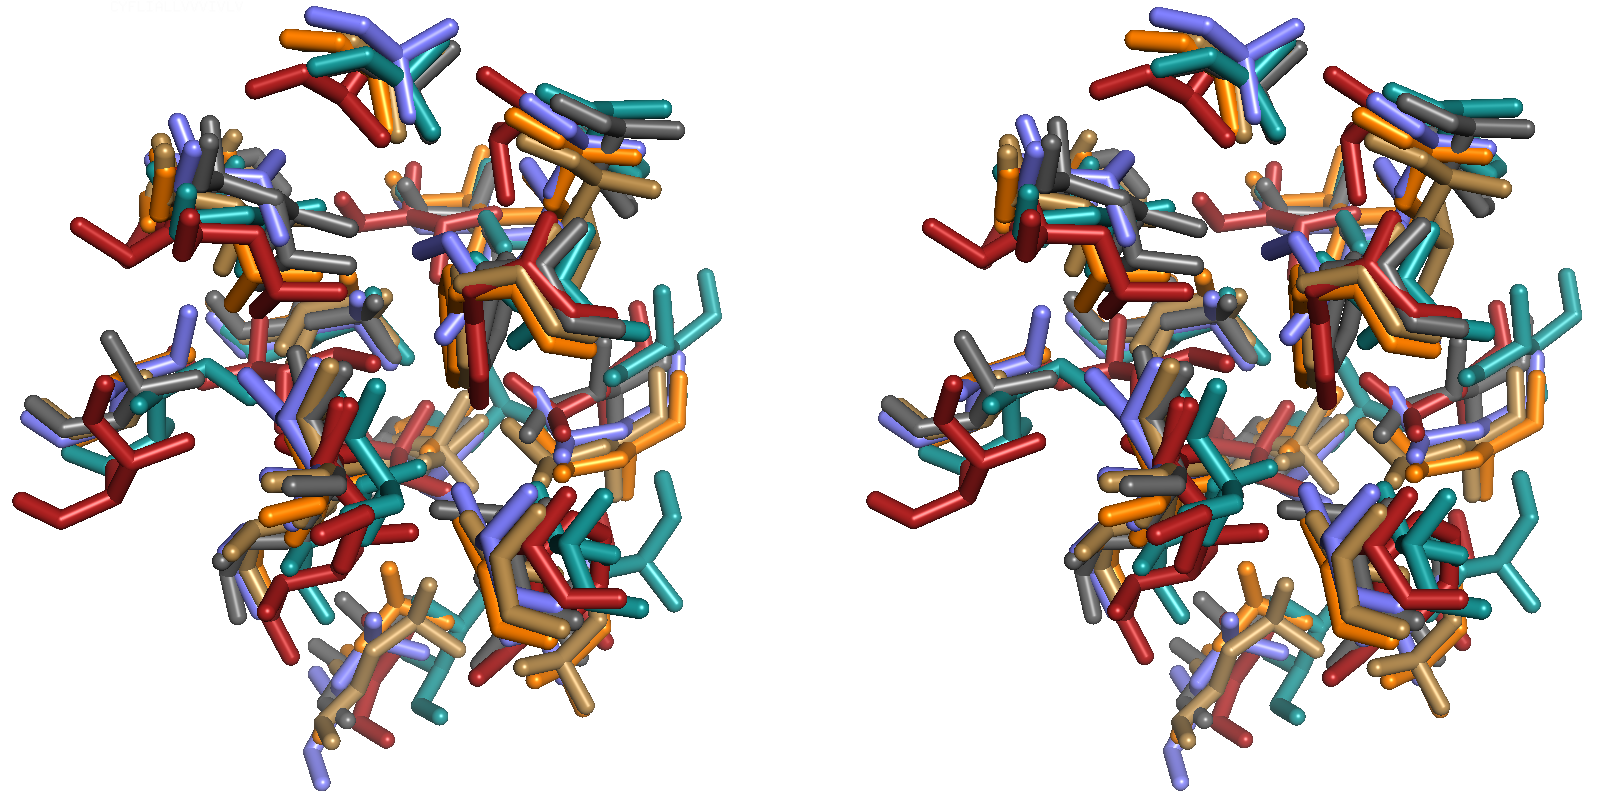
\includegraphics[width=17cm]{corePDZ.png} \\
     \end{tabular}
     \caption{le cœur PDZ sélectionné}
\label{graph:corePDZ}
   \end{figure}

    \clearpage

   \begin{figure}[t]
 \raggedleft{}
     \begin{tabular}{c}
       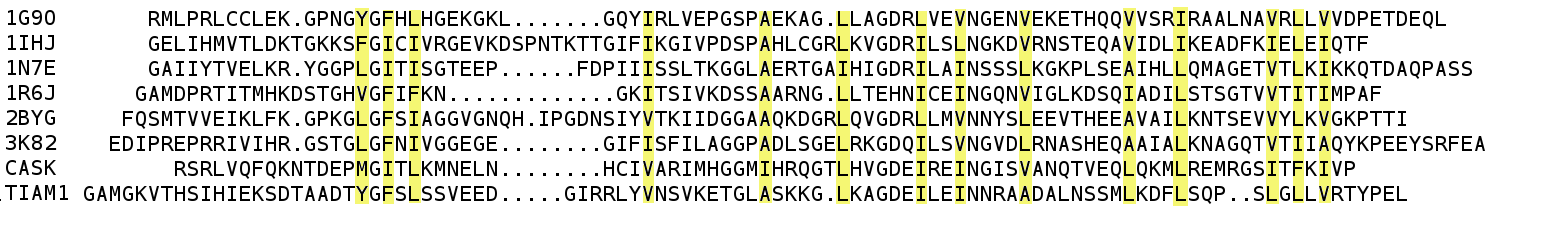
\includegraphics[width=18cm]{natives_alignees.png} \\
     \end{tabular}
     \caption{l'aligenement des séquences natives;le cœur PDZ sélectionné est en jaune.}
\label{graph:corePDZ}
   \end{figure}


    \clearpage
    \thispagestyle{empty}
   \begin{figure}[t]
     \centering
     \begin{tabular}{cc}
       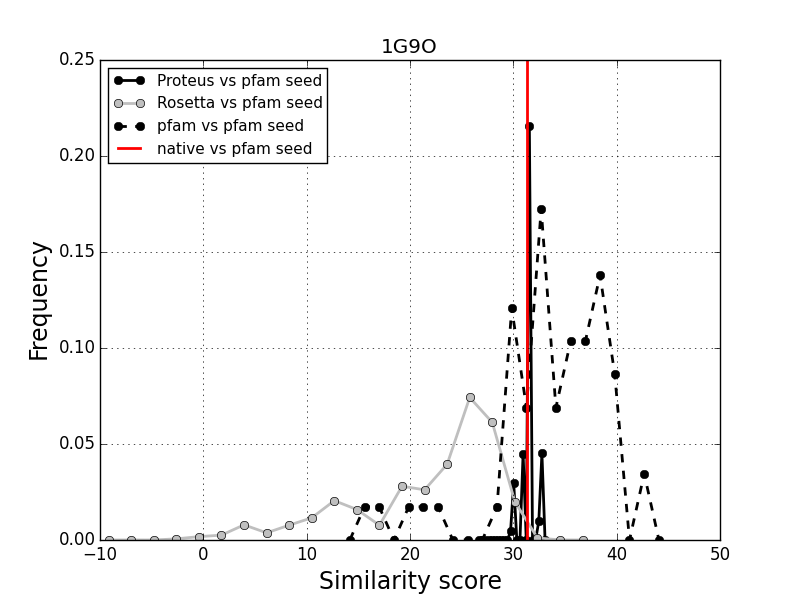
\includegraphics[width=8.4cm]{optGrad0/RP55/1G9O_core_simil.png} &
       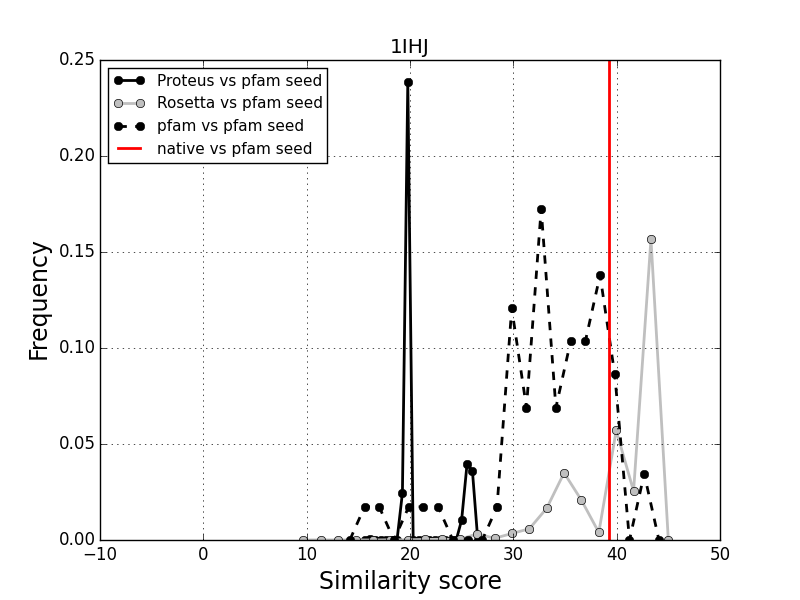
\includegraphics[width=8.4cm]{optGrad0/RP55/1IHJ_core_simil.png} \\
       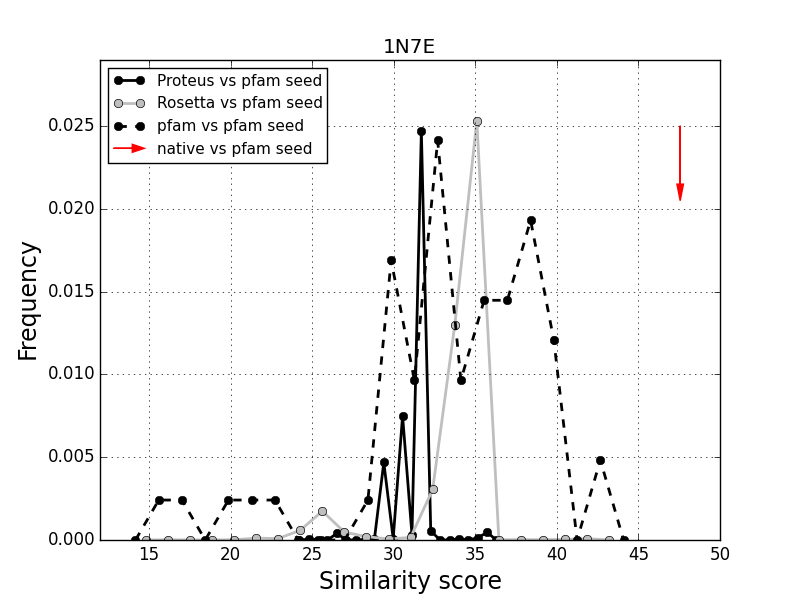
\includegraphics[width=8.4cm]{optGrad0/RP55/1N7E_core_simil.png} &
       \includegraphics[width=8.4cm]{optGrad0/RP55/1R6J_core_simil.png} \\
       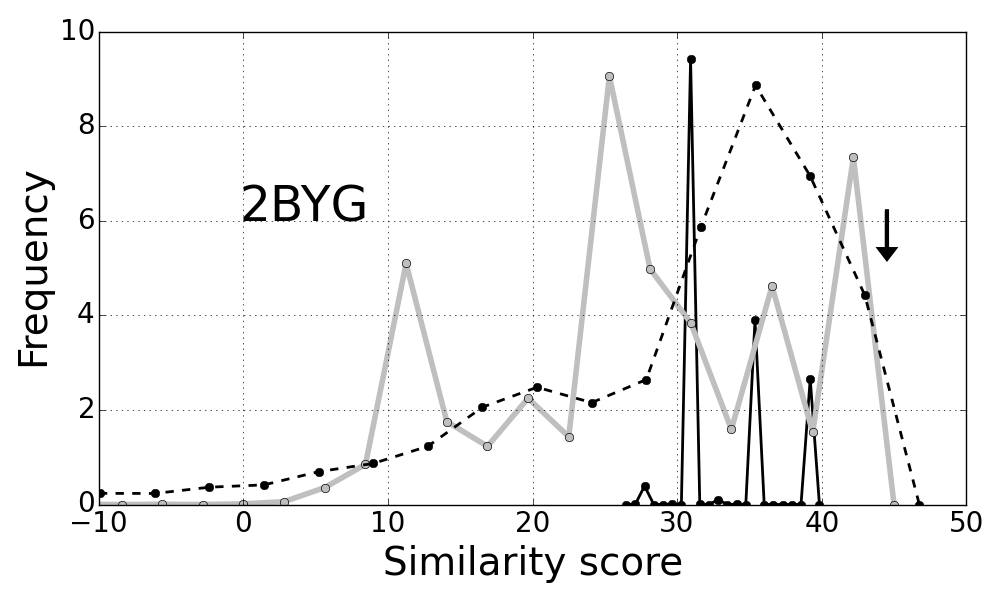
\includegraphics[width=8.4cm]{optGrad0/RP55/2BYG_core_simil.png} &
       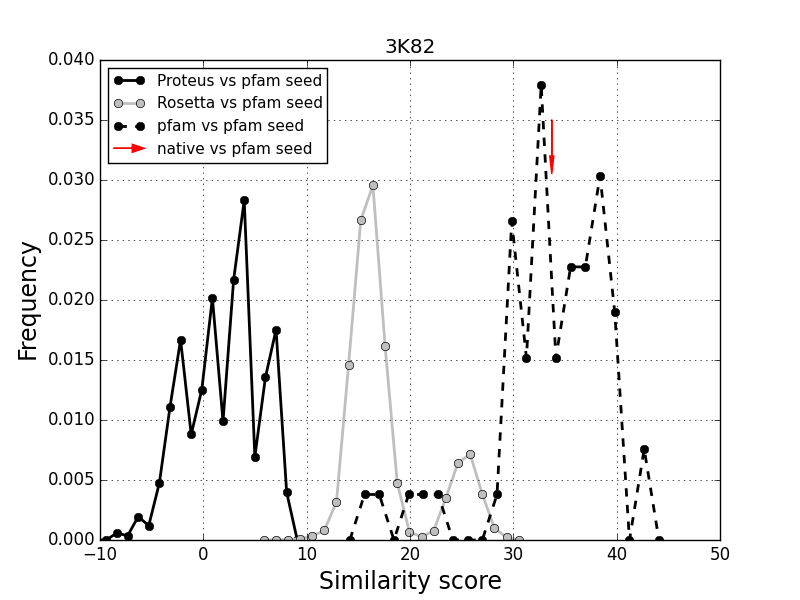
\includegraphics[width=8.4cm]{optGrad0/RP55/3K82_core_simil.png} \\
       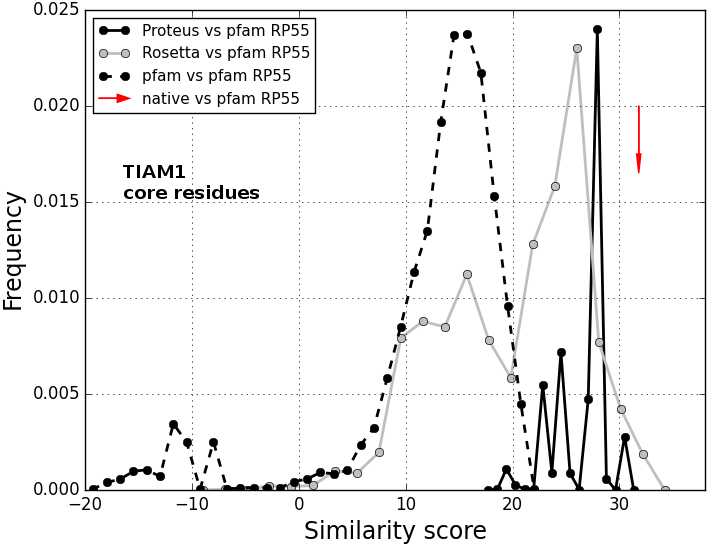
\includegraphics[width=8.4cm]{optGrad0/RP55/TIAM1_core_simil.png} &
       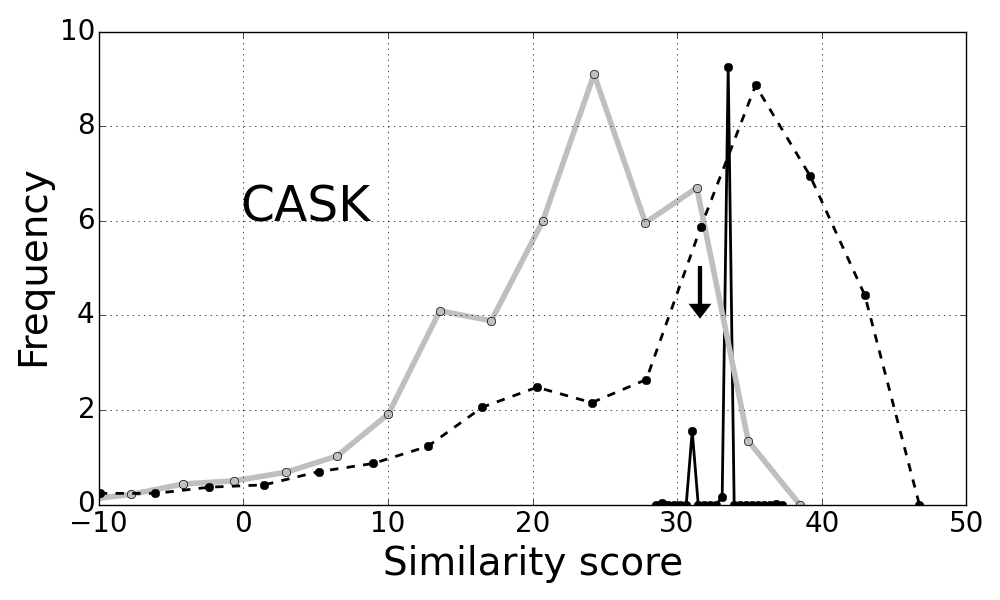
\includegraphics[width=8.4cm]{optGrad0/RP55/CASK_core_simil.png} \\ 
     \end{tabular}
%    \caption{Similarité des séquences Proteus(Enegie de référence sur 6 protéines) et Rosetta à l'alignement Pfam RP55, aux positions du cœur.}

\label{graph:Simil_Proteus_PDZ}
   \end{figure}

    \clearpage

    \begin{table}[!htbp]
      \centering

      \begin{tabular}{ccccccc}

        \toprule
        Protein & Proteus &  Proteus2 &  Proteus3 & Rosetta & Pfam seed \\
        \cmidrule{1-6}
        1G9O  & 1.40 & 1.42 & 1.47 & 1.45 & 3.15  \\
        1IHJ  & 1.38 & 1.46 & 1.51 & 1.55 & 3.06  \\
        1N7E  & 1.37 & 1.37 & 1.69 & 1.44 & 3.09  \\
        1R6J  & 1.39 & 1.44 & 1.53 & 1.43 & 3.03  \\
        2BYG  & 1.27 & 1.30 & 1.78 & 1.57 & 3.11  \\
        3K82  & 1.28 & 1.40 & 1.50 & 1.40 & 3.15  \\
        CASK  & 1.45 & 1.95 & 1.62 & 1.68 & 3.15  \\
        TIAM1 & 1.35 & 1.62 & 1.72 & 1.57 & 3.15  \\
        \bottomrule

      \end{tabular}      
      \caption{Moyenne de l'exponentiel de l'entropie sur les ensembles des positions des protéines}
\label{tab:Entropie_PDZ}      
    \end{table}

    \clearpage

    \begin{table}[!htbp]
      \centering

      \begin{tabular}{ccc}

        \toprule
        Sequences & Proteus & Rosetta \\
        \cmidrule{1-3}
        1G9O  & 1.38  & 1.45 \\
        1IHJ  & 1.37  & 1.55 \\
        1N7E  & 1.33  & 1.44 \\
        1R6J  & 1.39  & 1.43 \\
        2BYG  & 1.24  & 1.57 \\
        3K82  & 1.27  & 1.40 \\
        6prots & 2.42  & 2.88 \\
        TIAM1  & 1.55  & 1.57 \\
        CASK   & 1.22  & 1.69 \\

        \bottomrule

      \end{tabular}      
      \caption{Moyenne de l'exponentiel de l'entropie sur les ensembles des positions des protéines(énergies de référence optimisées sur six protéines)}
\label{tab:Entropie_PDZ}      
    \end{table}



    \begin{table}[!htbp]

\scalebox{0.85}{
      \begin{tabular}{ccccccccc}

        \toprule
        Protein & 1G9O & 1IHJ & 1N7E & 1R6J & 2BYG & 3K82 & CASK & TIAM1 \\
        \cmidrule{1-9}

        1G9O & 2e-66 (100)& 5e-10 (40)& 0.002 (25)& 3e-07 (25)& 2e-11 (35)& 1e-12 (30)& 5e-05 (25)& 9e-07(35)\\     
        1IHJ & 5e-10 (40) & 3e-68 (100)&  2e-07 (27)& no      & 2e-08 (27) & 9e-14 (46)& 4e-06 (35)& no    \\
        1N7E & 0.002 (25) & 2e-07 (27)&  3e-67 (100)& no       & 3e-14 (36) & 2e-10 (37)& 9e-12 (30)& 5e-05 (35)\\
        1R6J & 3e-07 (25) & no    &    no    & 1e-59 (100) &  no      & 1e-06 (32)& 0.007 (32)& no    \\
        2BYG & 2e-11 (35) & 2e-08 (27)&  3e-14 (37)& no      & 7e-71 (100) & 3e-15 (37)& 2e-07 (28)& 5e-05 (41)\\
        3K82 & 1e-12 (30) & 9e-14 (46)&  2e-10 (36)& 1e-06 (32)& 3e-15 (37) & 4e-70 (100)& 1e-07 (27)& 6e-04(33) \\
        Cask & 5e-05 (25) & 4e-06 (35)&  9e-12 (30)& 0.007 (32)& 2e-07 (28) & 1e-07 (27)& 7e-61 (100)& 5e-04(33) \\
        Tiam1 & 9e-07 (35)  &  no     &  5e-05 (35)& no      & 5e-05 (41) & 6e-04 (33)& 5e-04 (33)& 1e-68 (100)\\
        \bottomrule


      \end{tabular} 
}     
      \caption{E-value et pourcentage d'identité des alignements Blast croisés pour nos séquences PDZ. (no= pas de touche avec une E-value inférieure à 10)}
\label{tab:Xblast}      
    \end{table}



    \begin{table}[!htbp]
      \centering

      \begin{tabular}{ccccc}

        \toprule
        Sequences & Proteus & Rosetta & Proteus (inclus G et P) & Rosetta (inclus G et P)\\
        \cmidrule{1-5}
        1G9O  & 28 &  43 & 44 & 59 \\
        1IHJ  & 26 &  40 & 35 & 49 \\
        1N7E  & 33 &  48 & 50 & 65 \\
        1R6J  & 26 &  46 & 38 & 58 \\
        2BYG  & 28 &  46 & 42 & 61 \\
        3K82  & 36 &  52 & 54 & 70 \\
        TIAM1 & 18 &  25 & 28 & 30 \\
        CASK  & 17 &  28 & 28 &  39 \\

        \bottomrule

      \end{tabular}      
      \caption{Pourcentage d'identité moyen à la séquence native}
\label{tab:Entropie_PDZ}      
    \end{table}



\begin{table}[h]
  \raggedleft{}
  
  \begin{tabular}{cccccc}
    
    \toprule
    Protein & Match/seq & Superfamily & Superfamily & Family & Family \\
            & size      & Evalue      & success     & Evalue & success\\
    \cmidrule{1-6}
    1G9O  & 78/91 & 2.5e-3  & 10000 & 3.0e-3 & 10000 \\
    1IHJ  & 86/94 & 5.6e-7  & 10000 & 2.3e-3 & 10000 \\
    1N7E  & 81/95 & 1.1e-6  & 10000 & 2.4e-3 & 10000 \\
    1R6J  & 41/82 & 1.5     &  1350 & 2.6e-2 &  1350 \\
    2BYG  & 77/97 & 1.0e-2  & 10000 & 2.3e-3 & 10000 \\
    3K82  & 86/97 & 4.0e-16 & 10000 & 2.7e-3 & 10000 \\
    \cmidrule{1-6}
    CASK  & 72/83 & 2.3e-4  & 10000 & 1.5e-2 & 10000 \\
    TIAM1 & 43/94 & 1.28    & 442   & 4.0e-2 & 374 \\
    \cmidrule{1-6}
    1R6J-B & 70/82 & 1.4e-3    & 6664   & 4.0e-3 & 6664 \\
    \bottomrule        
  \end{tabular}   
  \caption{Résultats Superfamily pour les séquences Proteus avec le nouveau test Monte Carlo et énergies de référence optimisées sur l'ensemble réduit à six protéines}   
  \label{tab:superfamily_Old_MCtest}       
\end{table}




    \clearpage


   \begin{figure}[t]
     \centering
     \begin{tabular}{c}
       \includegraphics[width=17cm]{result/1G9O.png} \\
     \end{tabular}
     \caption{Sélection de séquences proteus 1G9O }
\label{result:1G9O}
   \end{figure}

   \begin{figure}[t]
     \centering
     \begin{tabular}{c}
       \includegraphics[width=17cm]{result/1IHJ.png} \\
     \end{tabular}
     \caption{Sélection de séquences proteus 1IHJ }
\label{result:1IHJ}
   \end{figure}

    \clearpage
   \begin{figure}[t]
     \centering
     \begin{tabular}{c}
       \includegraphics[width=17cm]{result/1N7E.png} \\
     \end{tabular}
     \caption{Sélection de séquences proteus 1N7E }
\label{result:1N7E}
   \end{figure}

   \begin{figure}[t]
     \centering
     \begin{tabular}{c}
       \includegraphics[width=17cm]{result/1R6J.png} \\
     \end{tabular}
     \caption{Sélection de séquences proteus 1R6J }
\label{result:1R6J}
   \end{figure}

    \clearpage

   \begin{figure}[t]
     \centering
     \begin{tabular}{c}
       \includegraphics[width=17cm]{result/2BYG.png} \\
     \end{tabular}
     \caption{Sélection de séquences proteus 2BYG }
\label{result:2BYG}
   \end{figure}

   \begin{figure}[t]
     \centering
     \begin{tabular}{c}
       \includegraphics[width=17cm]{result/3K82.png} \\
     \end{tabular}
     \caption{Sélection de séquences proteus 3K82 }
\label{result:3K82}
   \end{figure}

    \clearpage

   \begin{figure}[t]
     \centering
     \begin{tabular}{c}
       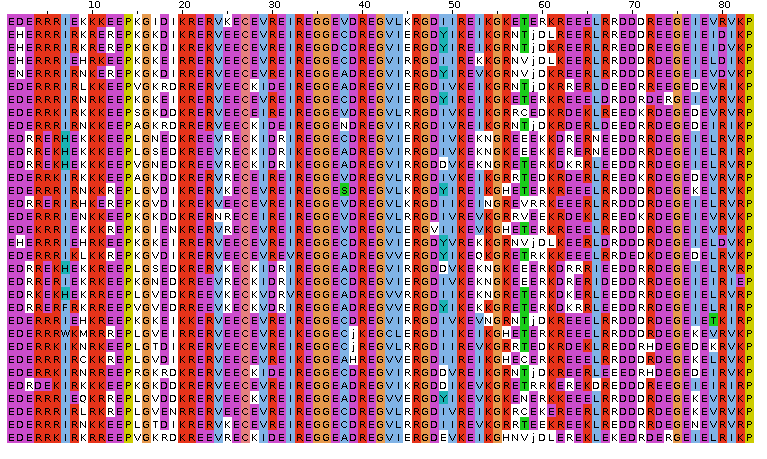
\includegraphics[width=17cm]{result/CASK.png} \\
     \end{tabular}
     \caption{Sélection de séquences proteus CASK }
\label{result:CASK}
   \end{figure}

   \begin{figure}[t]
     \centering
     \begin{tabular}{c}
       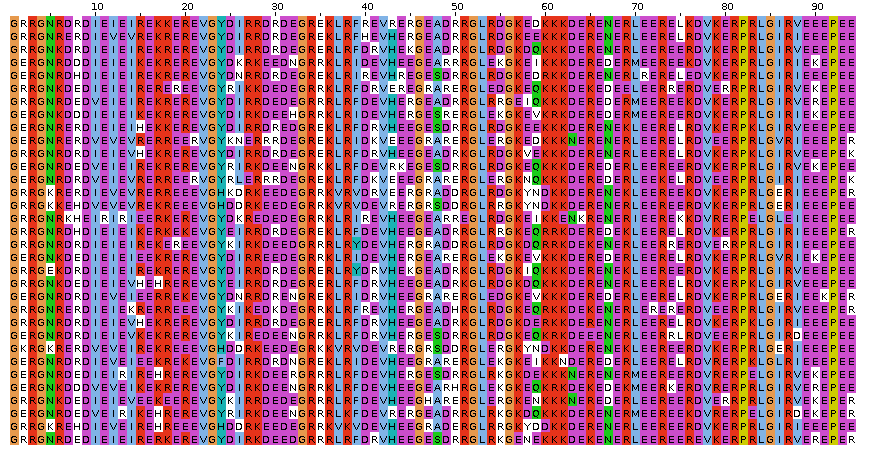
\includegraphics[width=17cm]{result/TIAM1.png} \\
     \end{tabular}
     \caption{Sélection de séquences proteus TIAM1 }
\label{result:TIAM1}
   \end{figure}

    \clearpage


   \begin{figure}[t]
     \centering
     \begin{tabular}{c}
       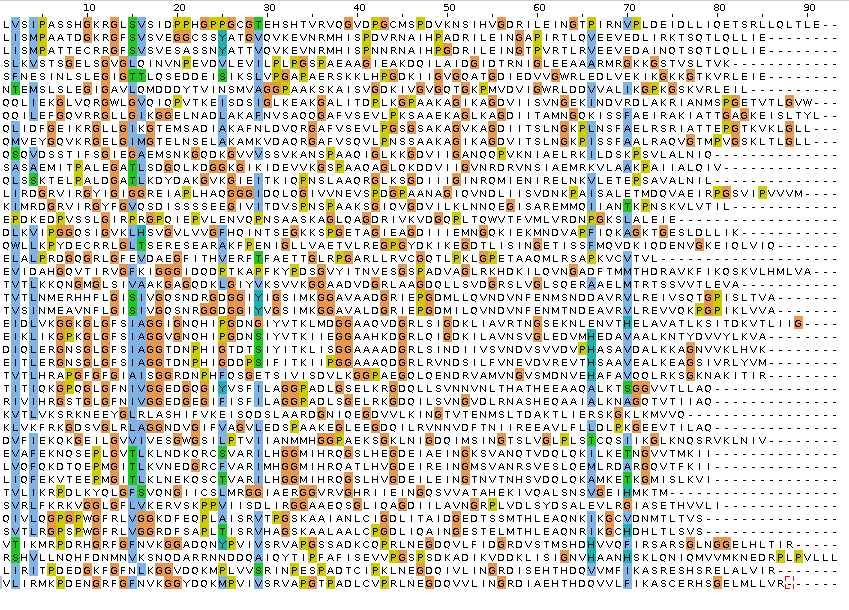
\includegraphics[width=17cm]{result/PDZ.png} \\
     \end{tabular}
     \caption{Les séquences de l'alignement PDZ seed de Pfam}
\label{result:PDZ_seed}
   \end{figure}

    \clearpage
\begin{landscape}

   \begin{figure}[t]
     \centering
     \begin{tabular}{c}
       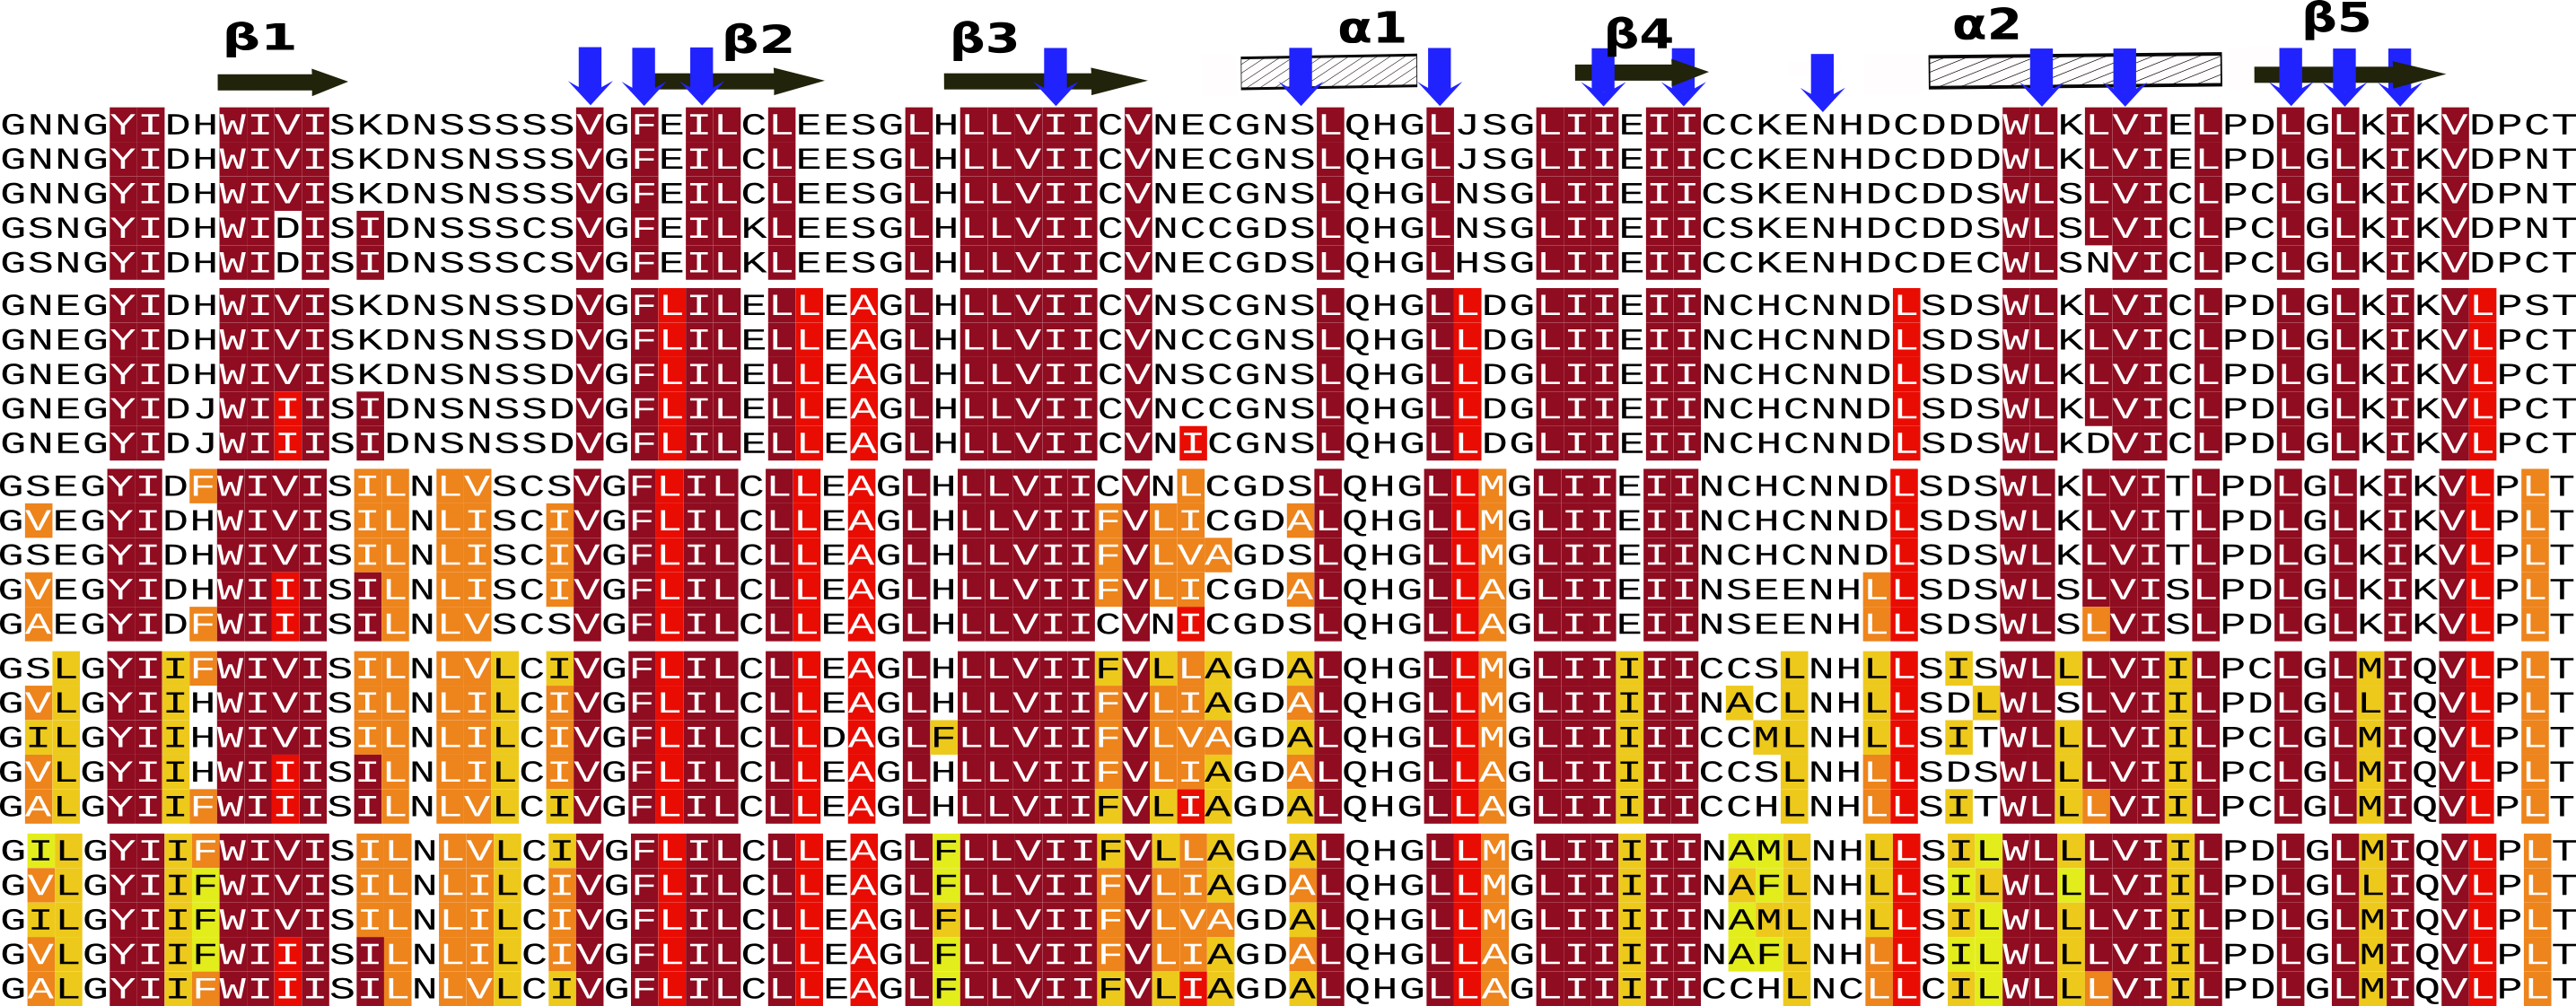
\includegraphics[width=18cm]{boost_hydro/modelA/alignTIAM1.png} \\
     \end{tabular}
%     \caption{Séquences Tiam1 obtenues avec un delta des énergies de références à -0.4,-0.2,0,0.2 et 0.4. Les hydrophobes sont représentés par un dégradé allant du rouge foncé au jaune clair.}
\label{result:PDZ_seed}
   \end{figure}

   \begin{figure}[t]
     \centering
     \begin{tabular}{c}
       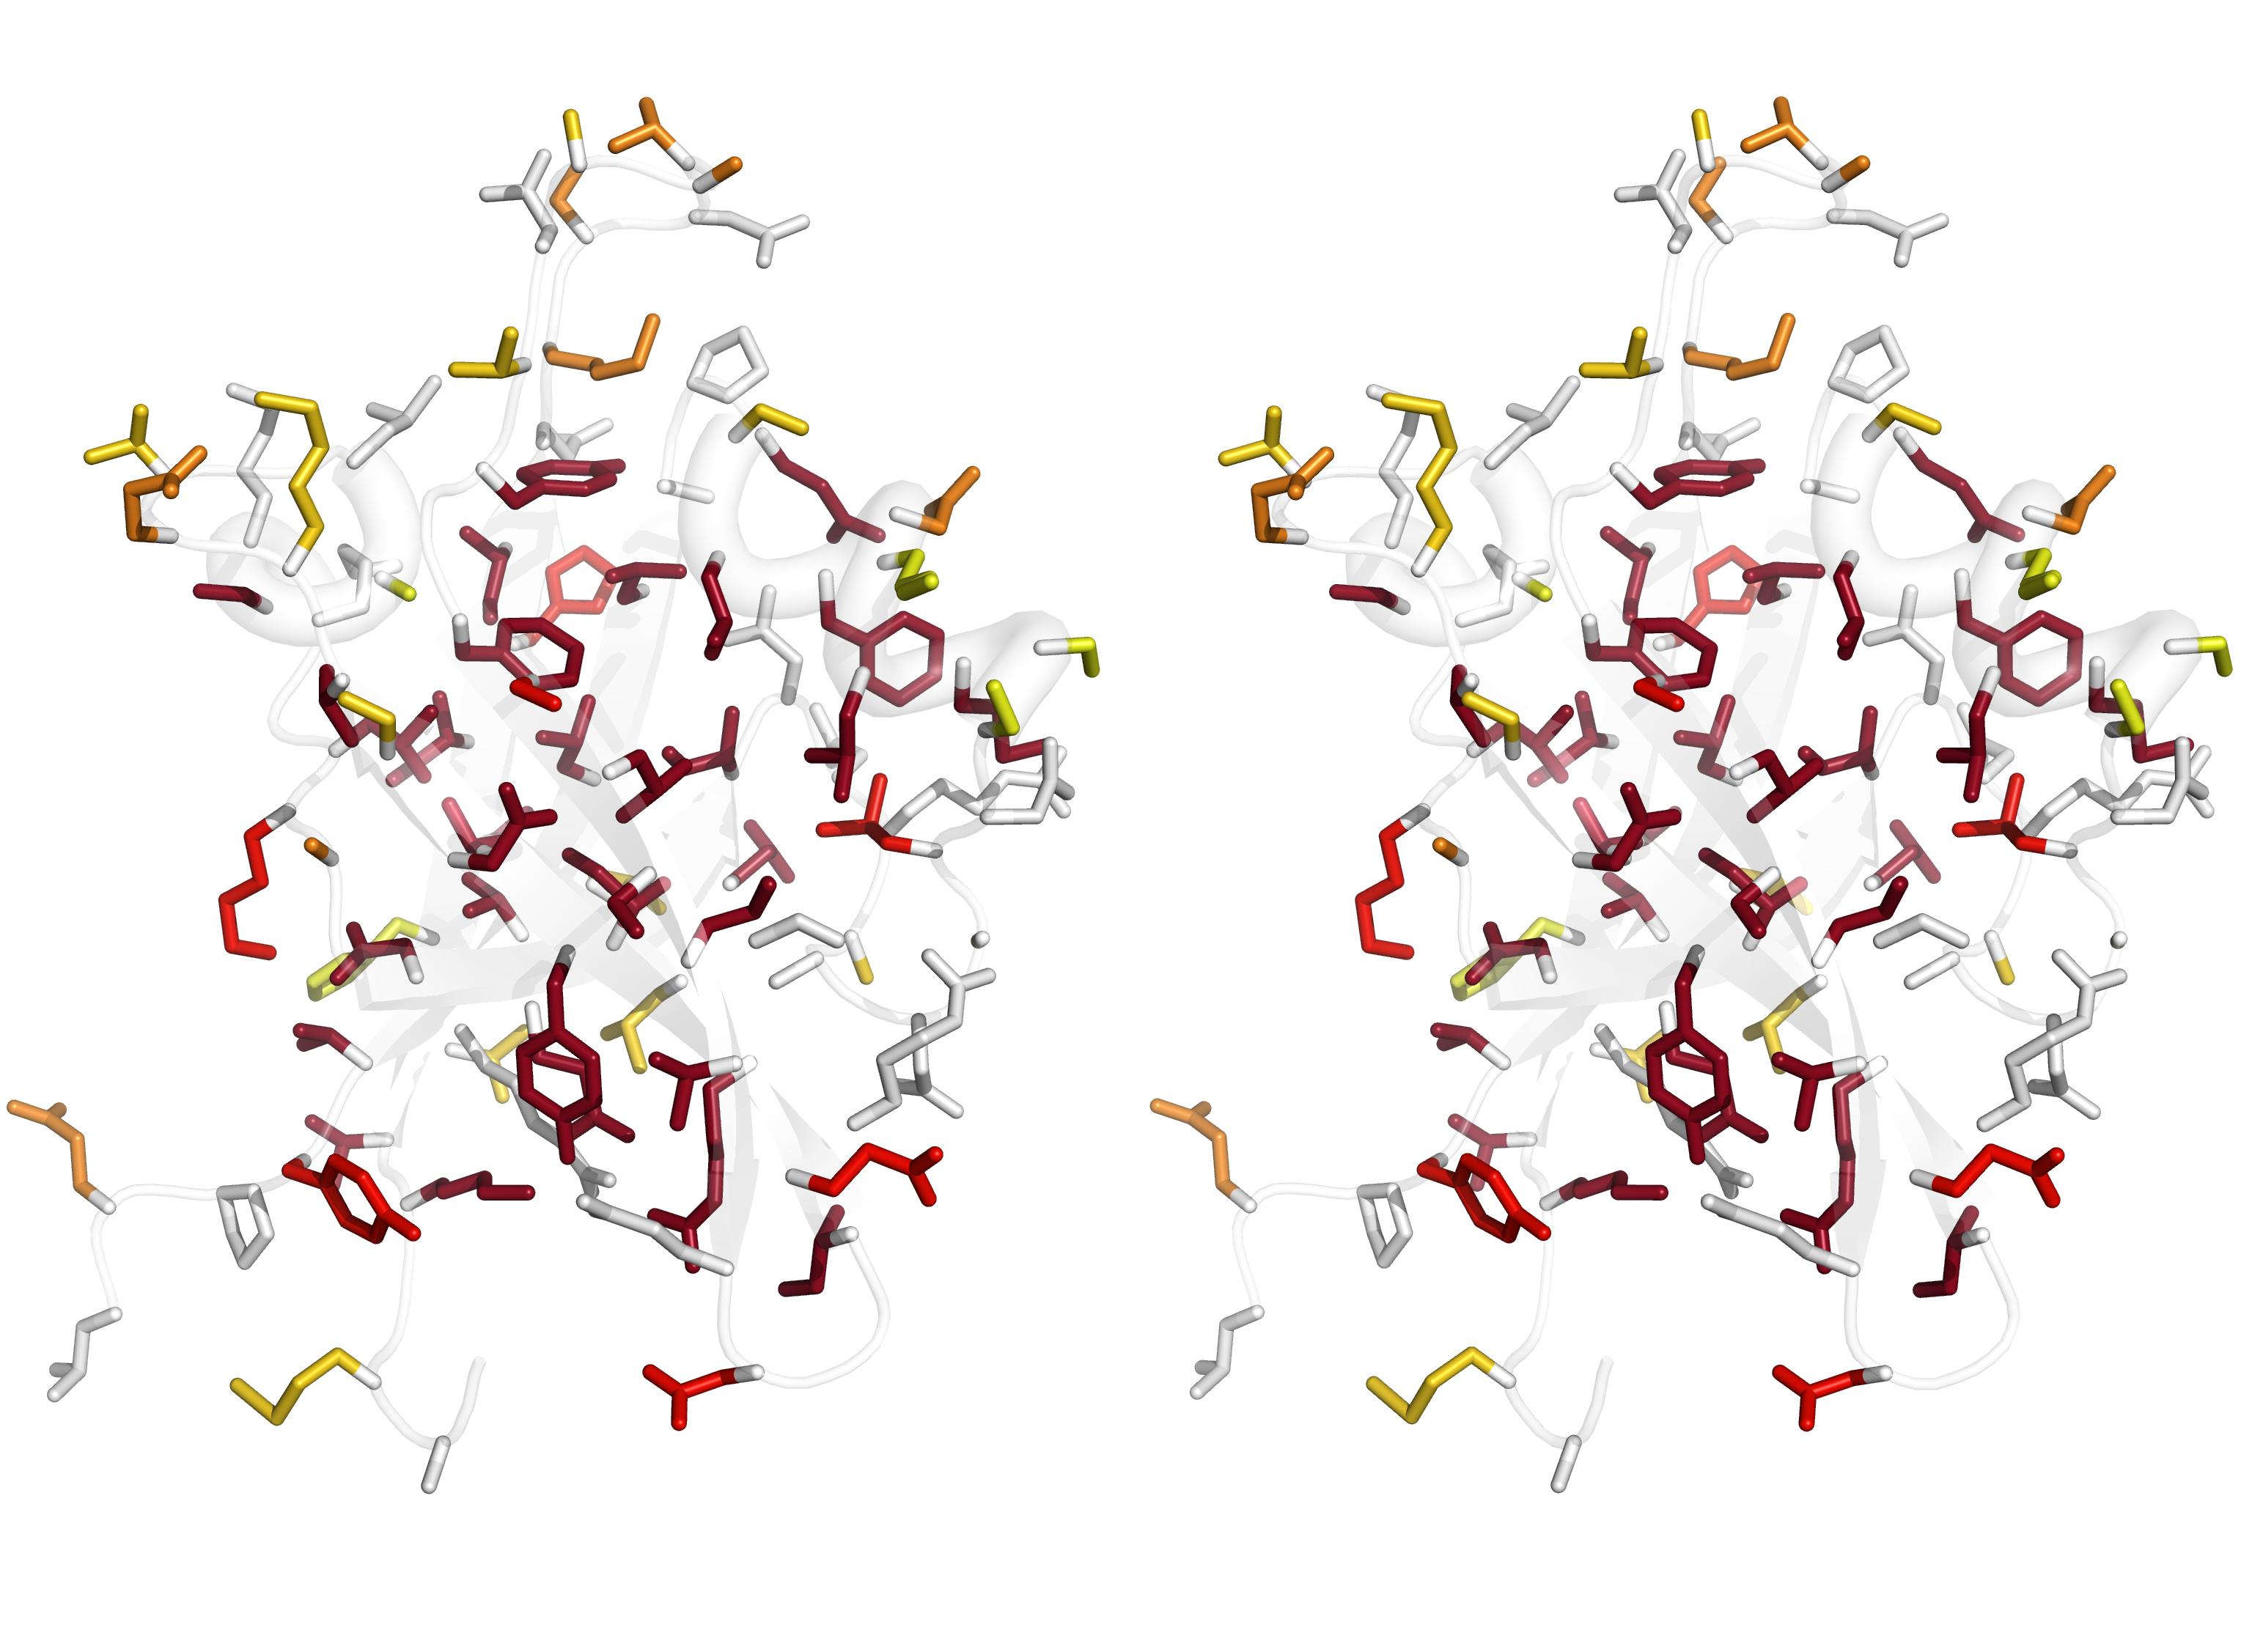
\includegraphics[width=9cm]{boost_hydro/modelA/structureTIAM1.png} \\
     \end{tabular}

     \caption{\small Séquences Tiam1 obtenues avec un delta des énergies de références à -0.4,-0.2,0,0.2 et 0.4 et la struture native.Les hydrophobes pour des deltas de -0.4,-0.2,0,0.2 et 0.4 sont représentés par un dégradé allant du rouge foncé au jaune clair.}

\label{result:PDZ_seed}
   \end{figure}

\end{landscape}


\clearpage
\thispagestyle{empty}
%\setcounter{page}{0}
\begin{landscape}

   \begin{figure}[t]
     \centering
     \begin{tabular}{l}
       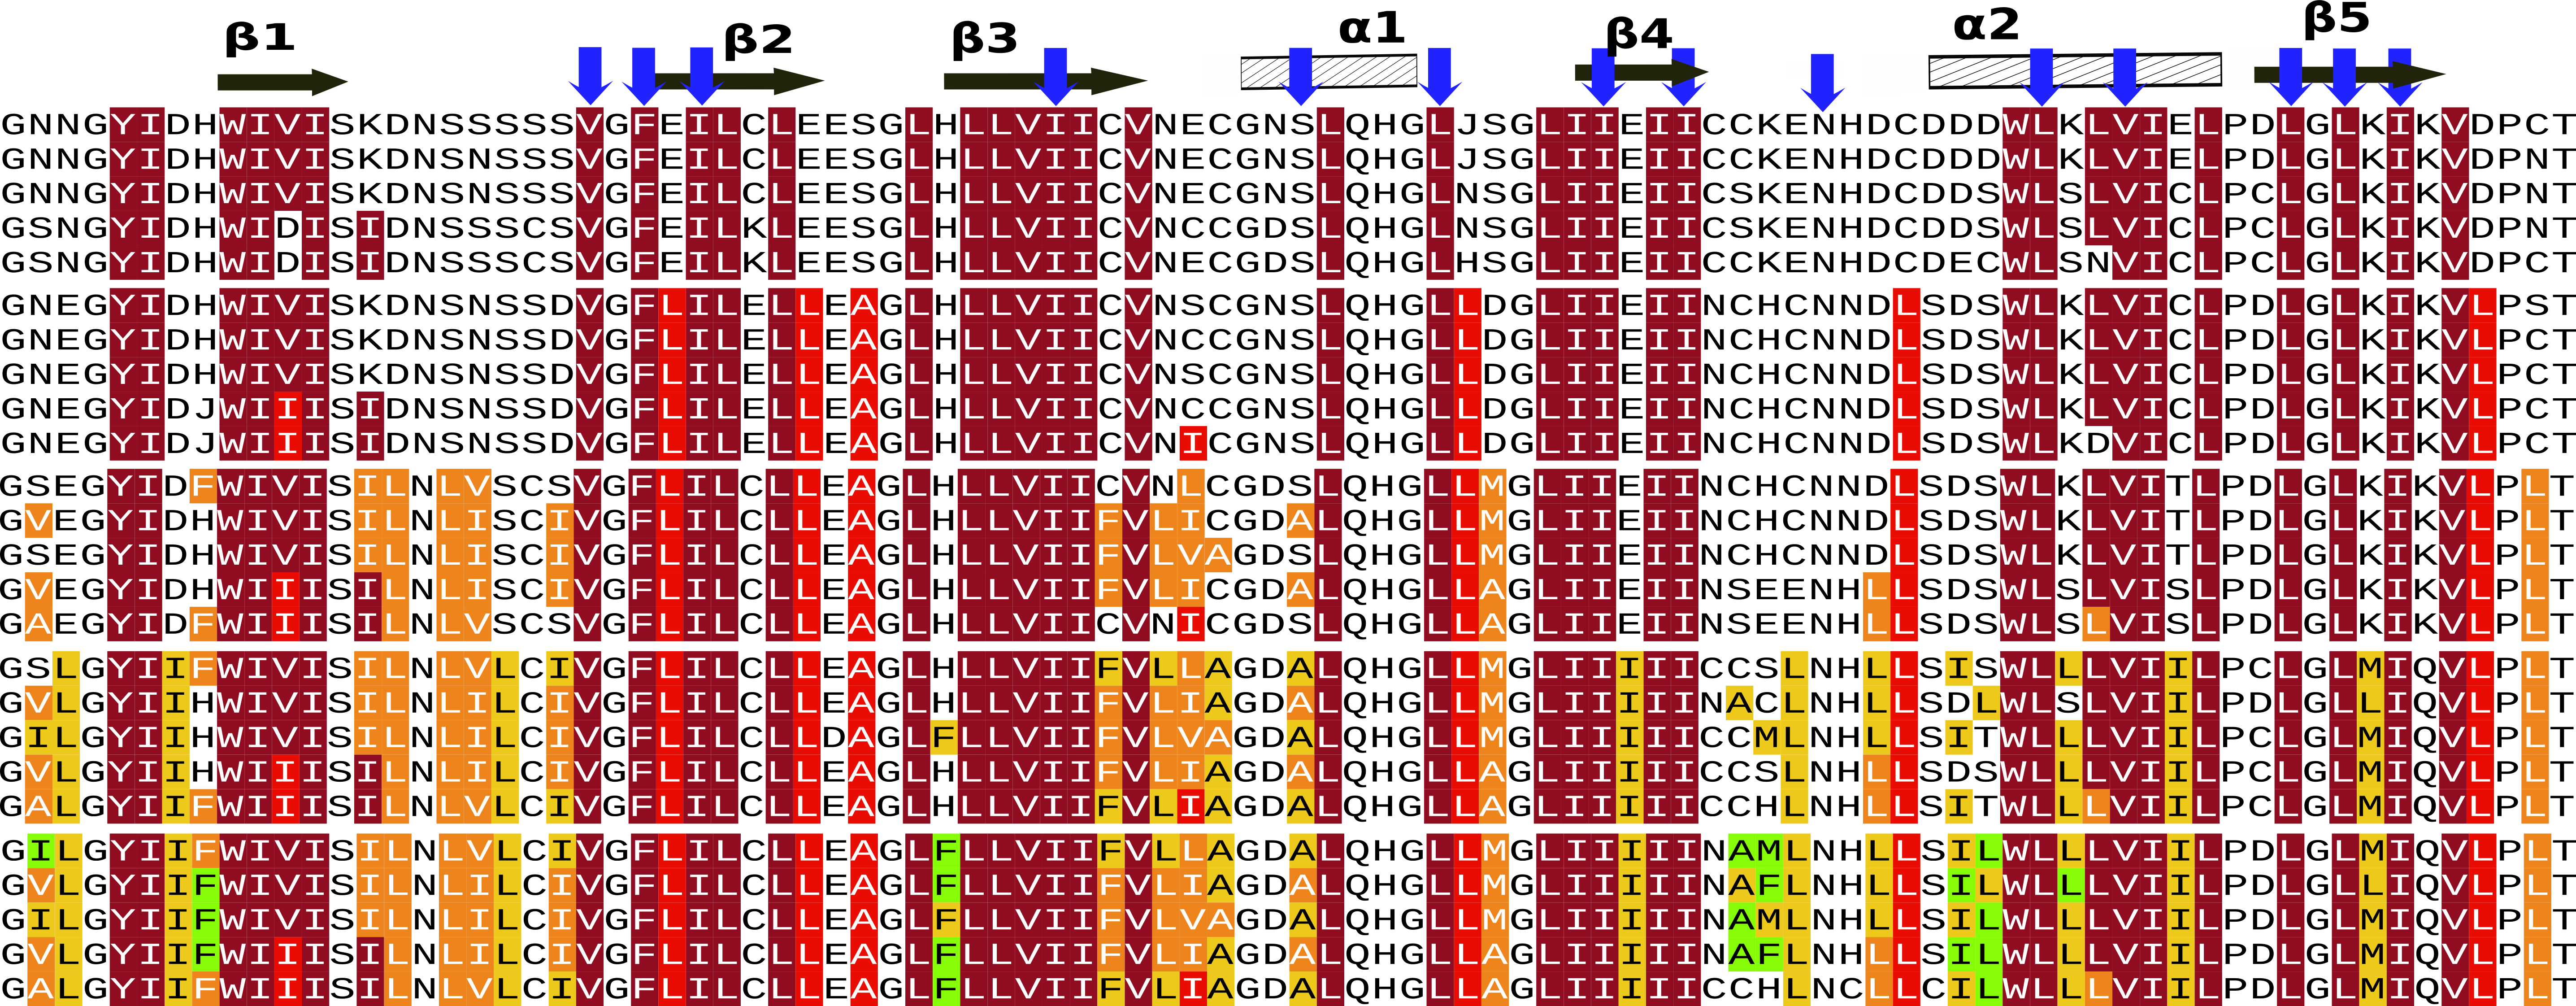
\includegraphics[width=18cm]{boost_hydro/modelA/alignTIAM1_V2.png} \\
       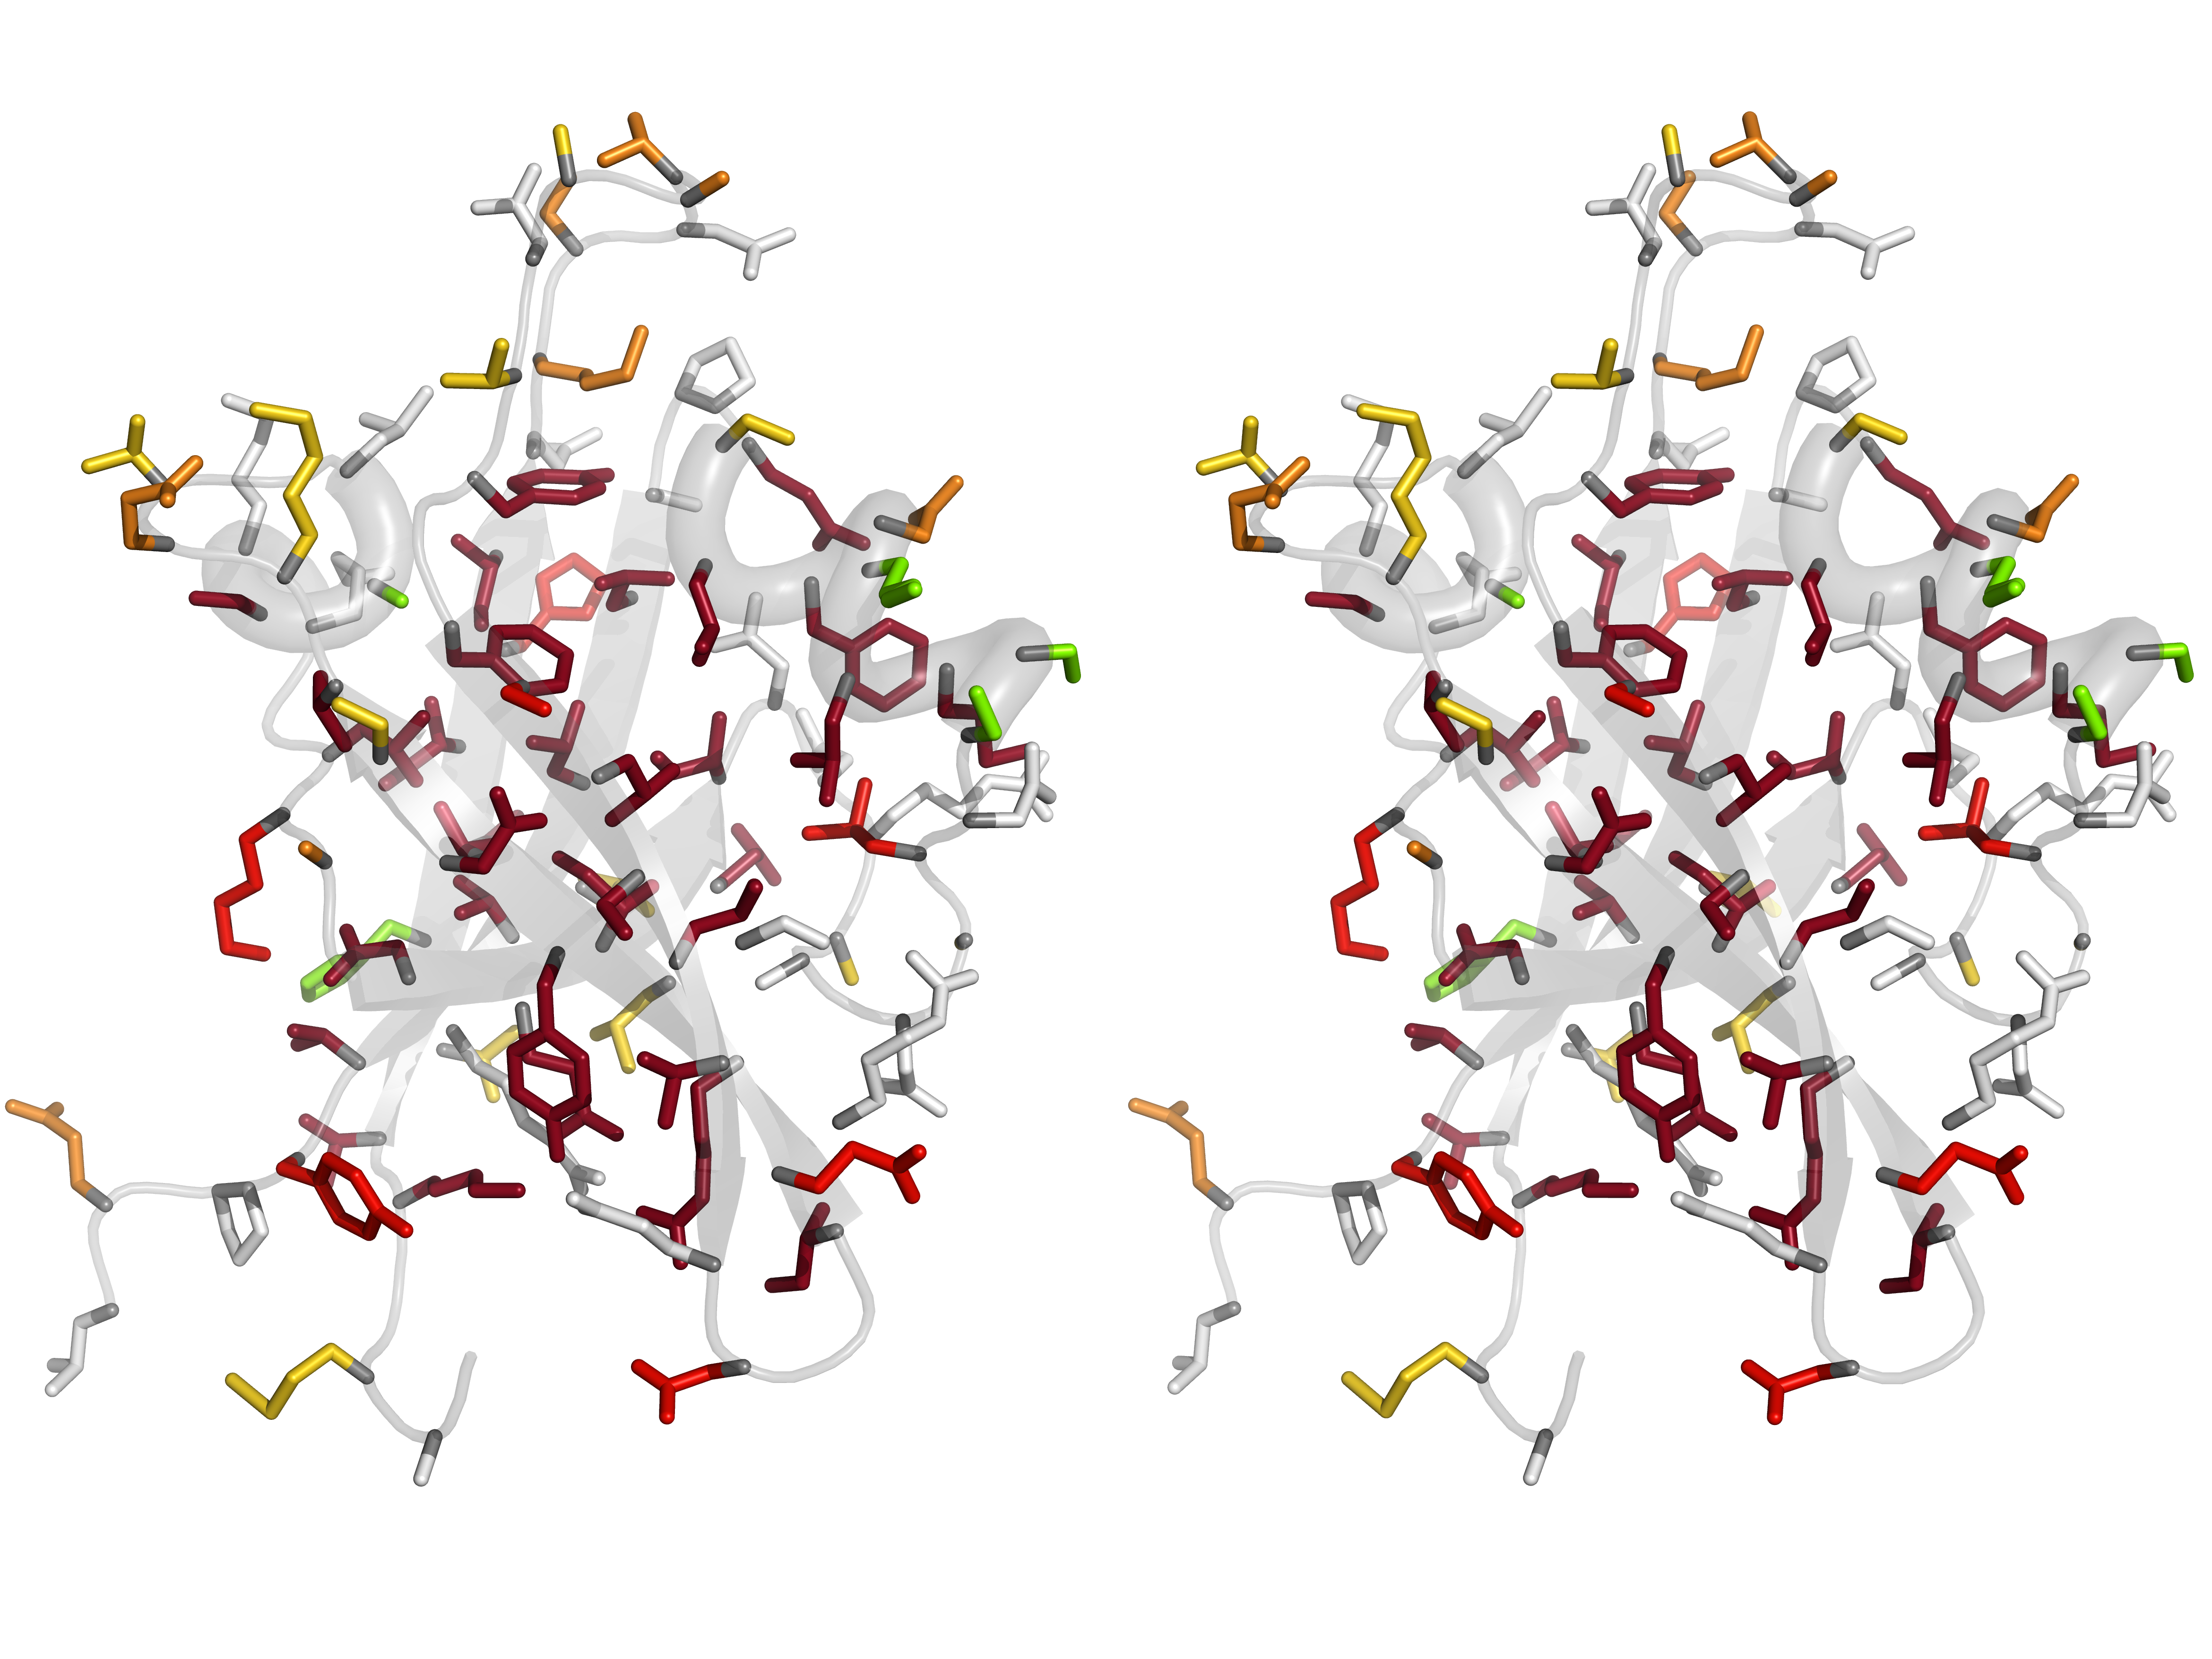
\includegraphics[width=11cm]{boost_hydro/modelA/structureTIAM1_V2.png} \\
     \end{tabular}
%     \caption{Séquences Tiam1 obtenues avec un delta des énergies de références à -0.4,-0.2,0,0.2 et 0.4. Les hydrophobes sont représentés par un dégradé allant du rouge foncé au jaune clair.}
\label{result:PDZ_seed}
   \end{figure}
%     \caption{\small Séquences Tiam1 obtenues avec un delta des énergies de références à -0.4,-0.2,0,0.2 et 0.4 et la struture native.Les hydrophobes pour des deltas de -0.4,-0.2,0,0.2 et 0.4 sont représentés par un dégradé allant du rouge foncé au jaune clair.}

\label{result:PDZ_seed}
   \end{figure}

\end{landscape}


    \clearpage

\begin{landscape}

   \begin{figure}[t]
     \centering
     \begin{tabular}{c}
       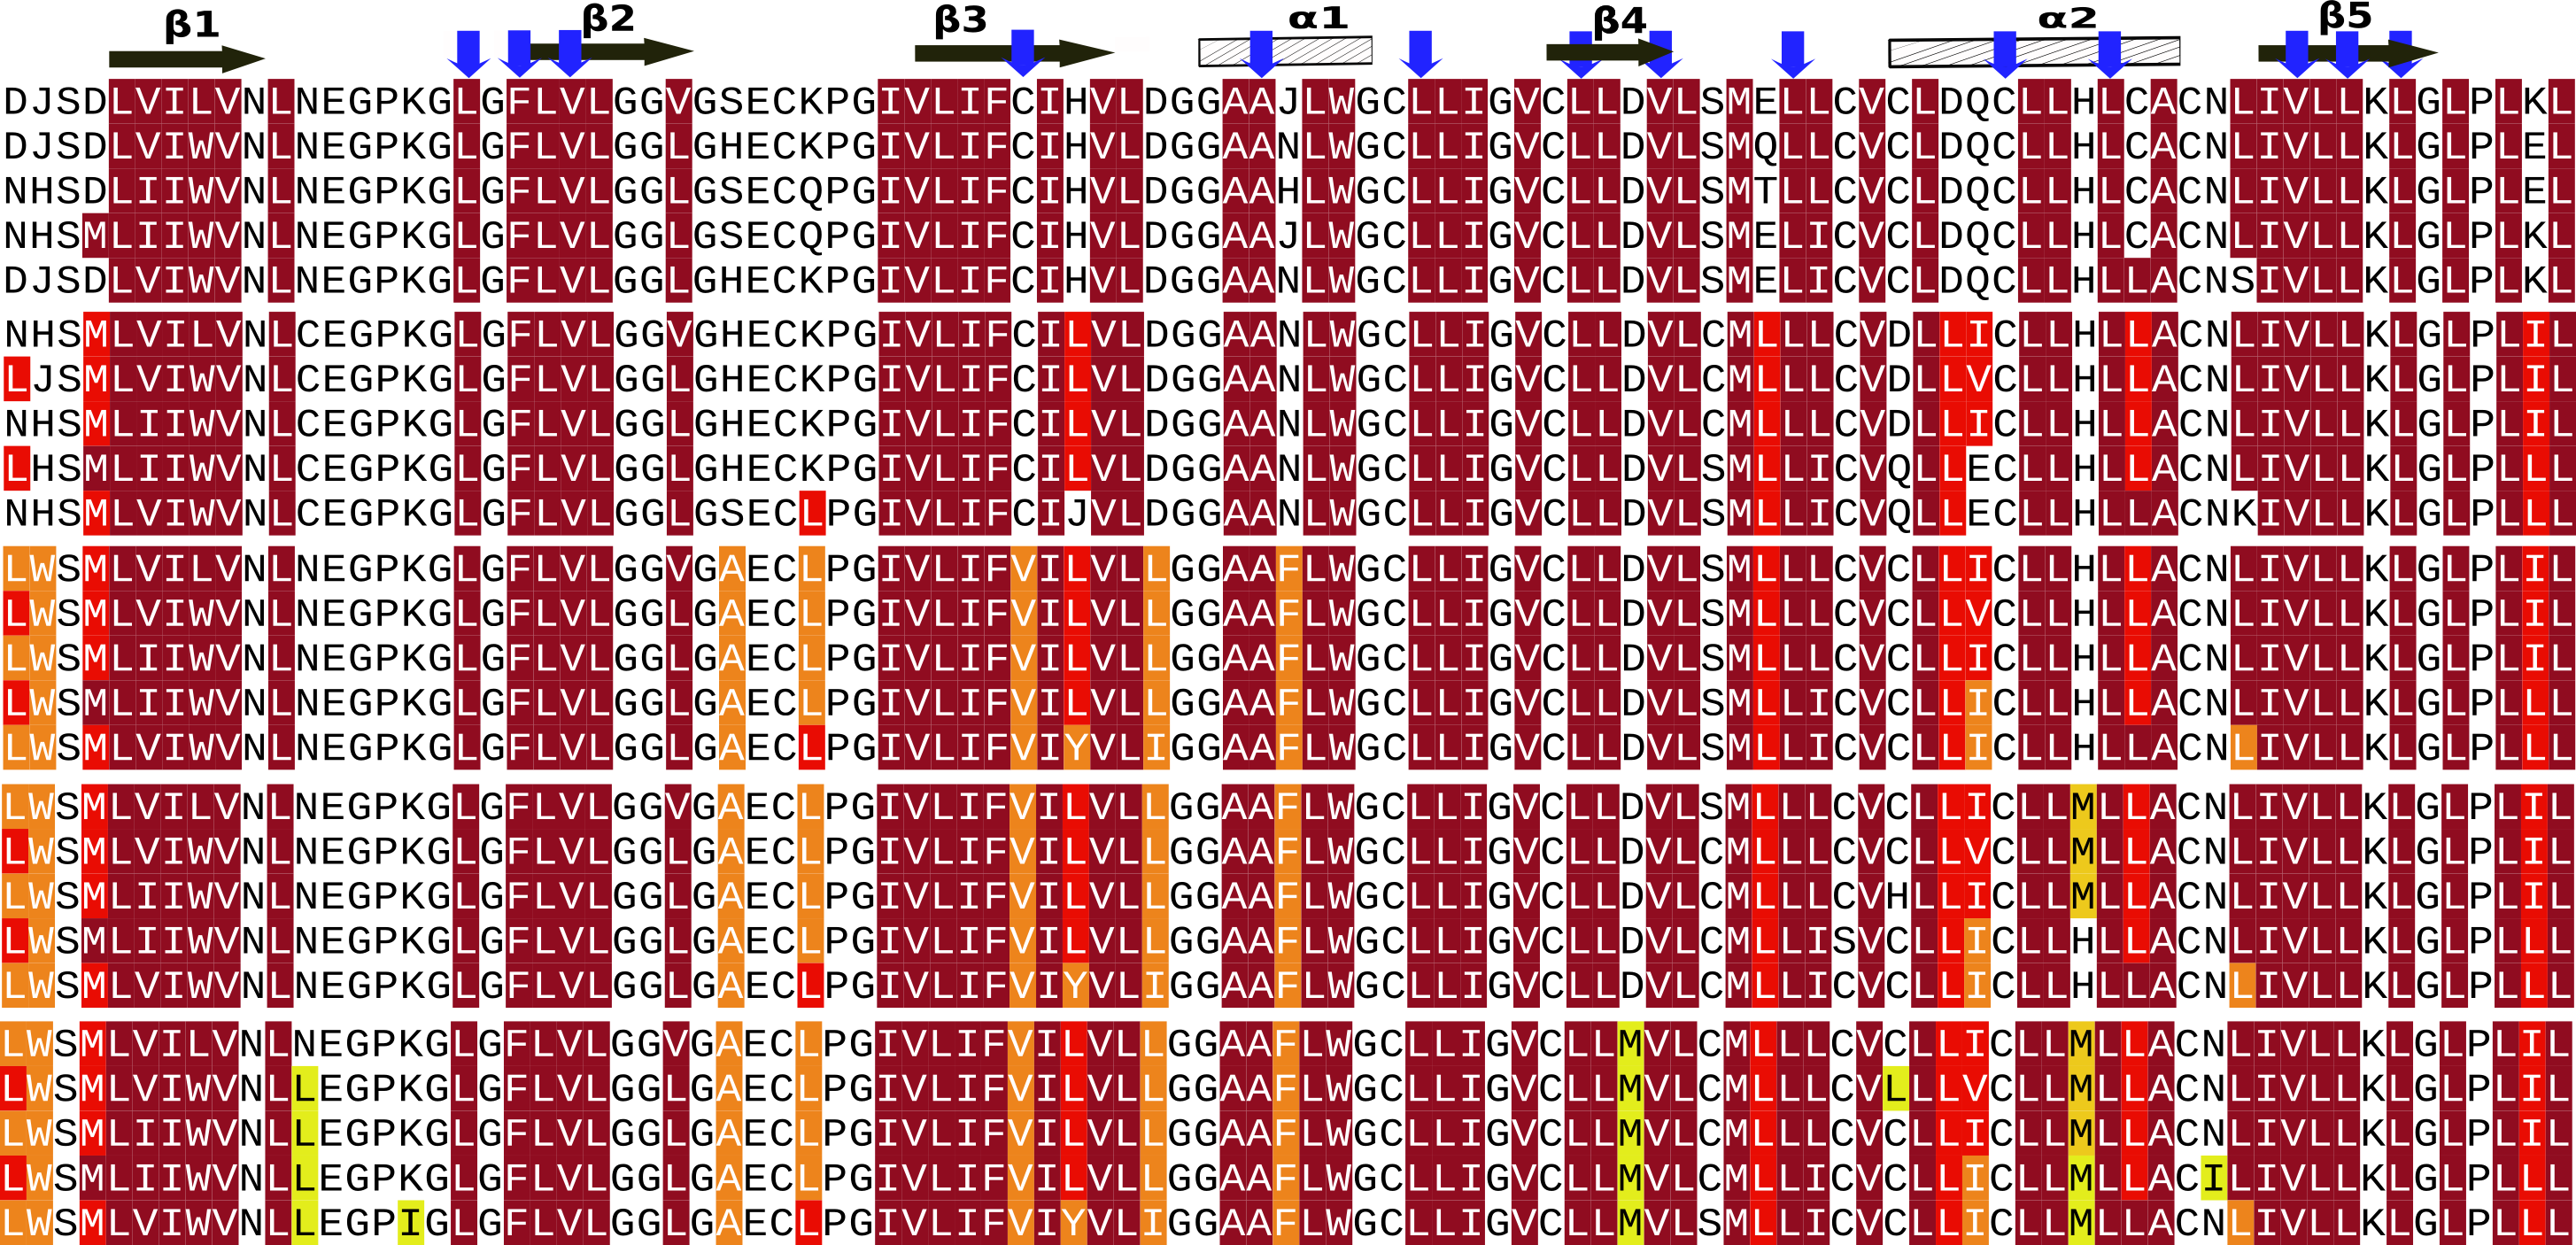
\includegraphics[width=14cm]{boost_hydro/modelA/align2BYG.png} \\
     \end{tabular}
%     \caption{Séquences Tiam1 obtenues avec un delta des énergies de références à -0.4,-0.2,0,0.2 et 0.4. Les hydrophobes sont représentés par un dégradé allant du rouge foncé au jaune clair.}
\label{result:PDZ_seed}
   \end{figure}

   \begin{figure}[t]
     \centering
     \begin{tabular}{c}
       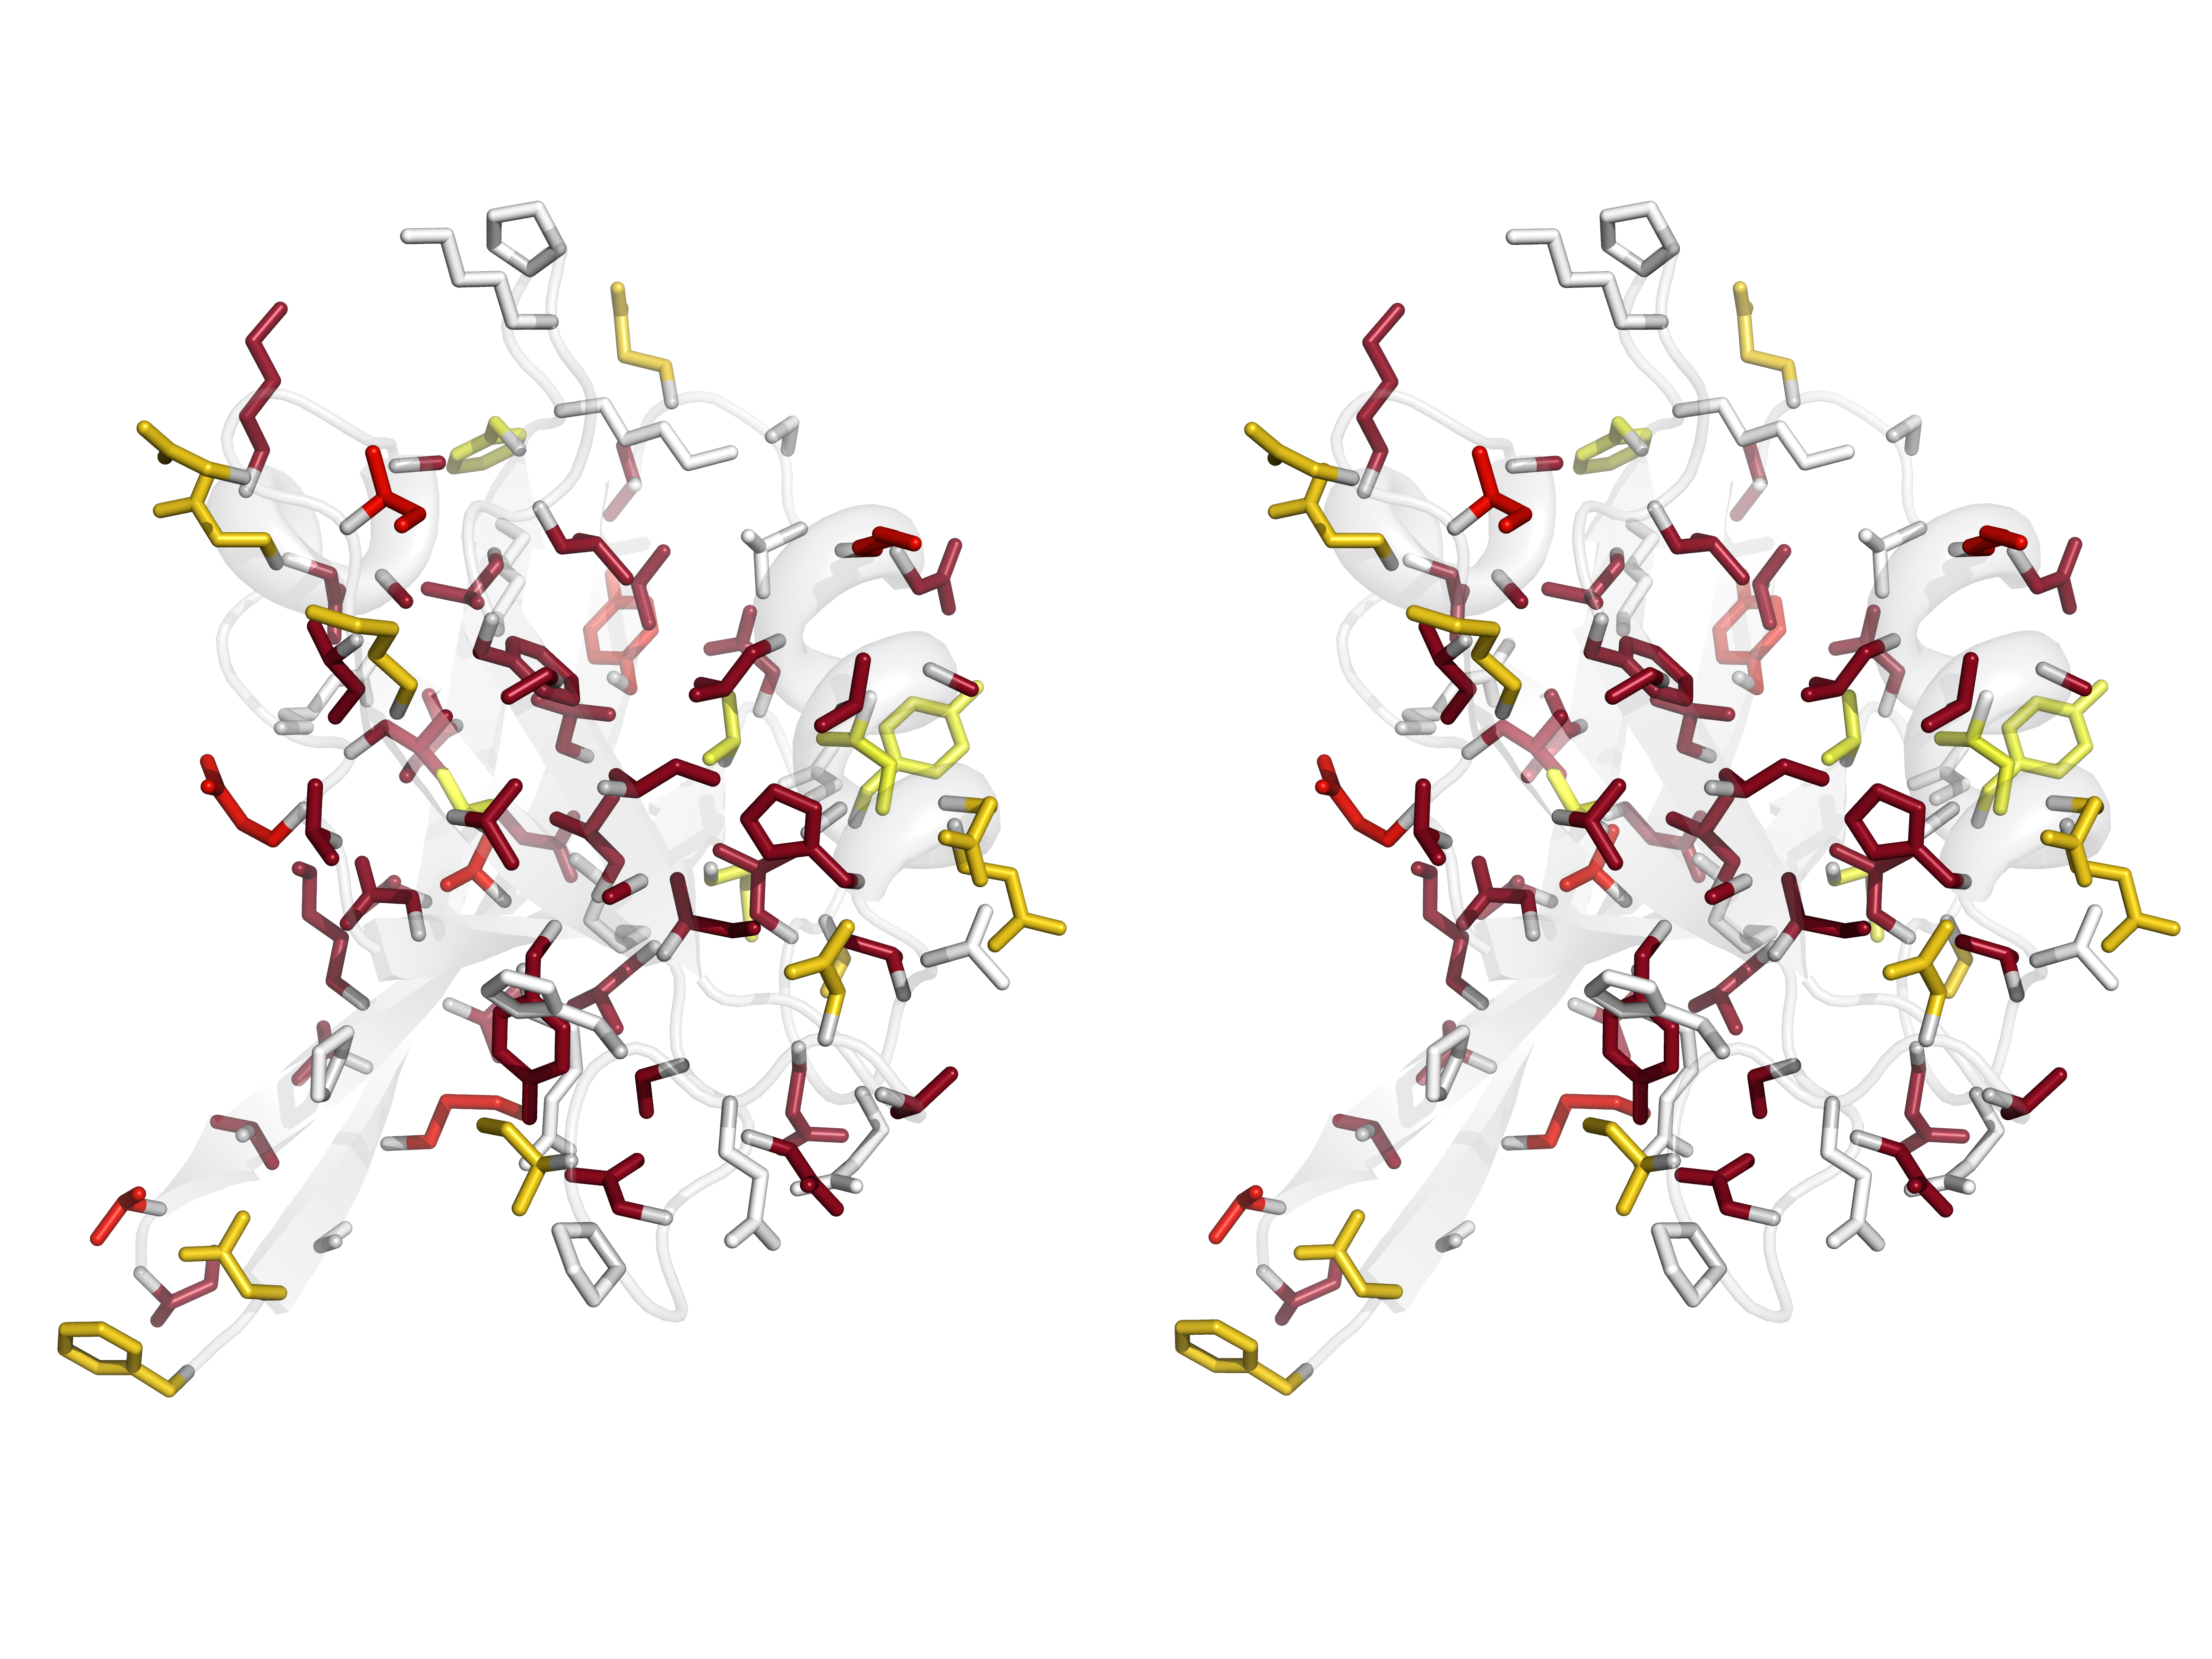
\includegraphics[width=9cm]{boost_hydro/modelA/structure2BYG.png} \\
     \end{tabular}

     \caption{\small Séquences 2BYG.}

\label{result:PDZ_seed}
   \end{figure}

\end{landscape}


   \clearpage

\begin{landscape}

   \begin{figure}[t]
     \centering
     \begin{tabular}{c}
       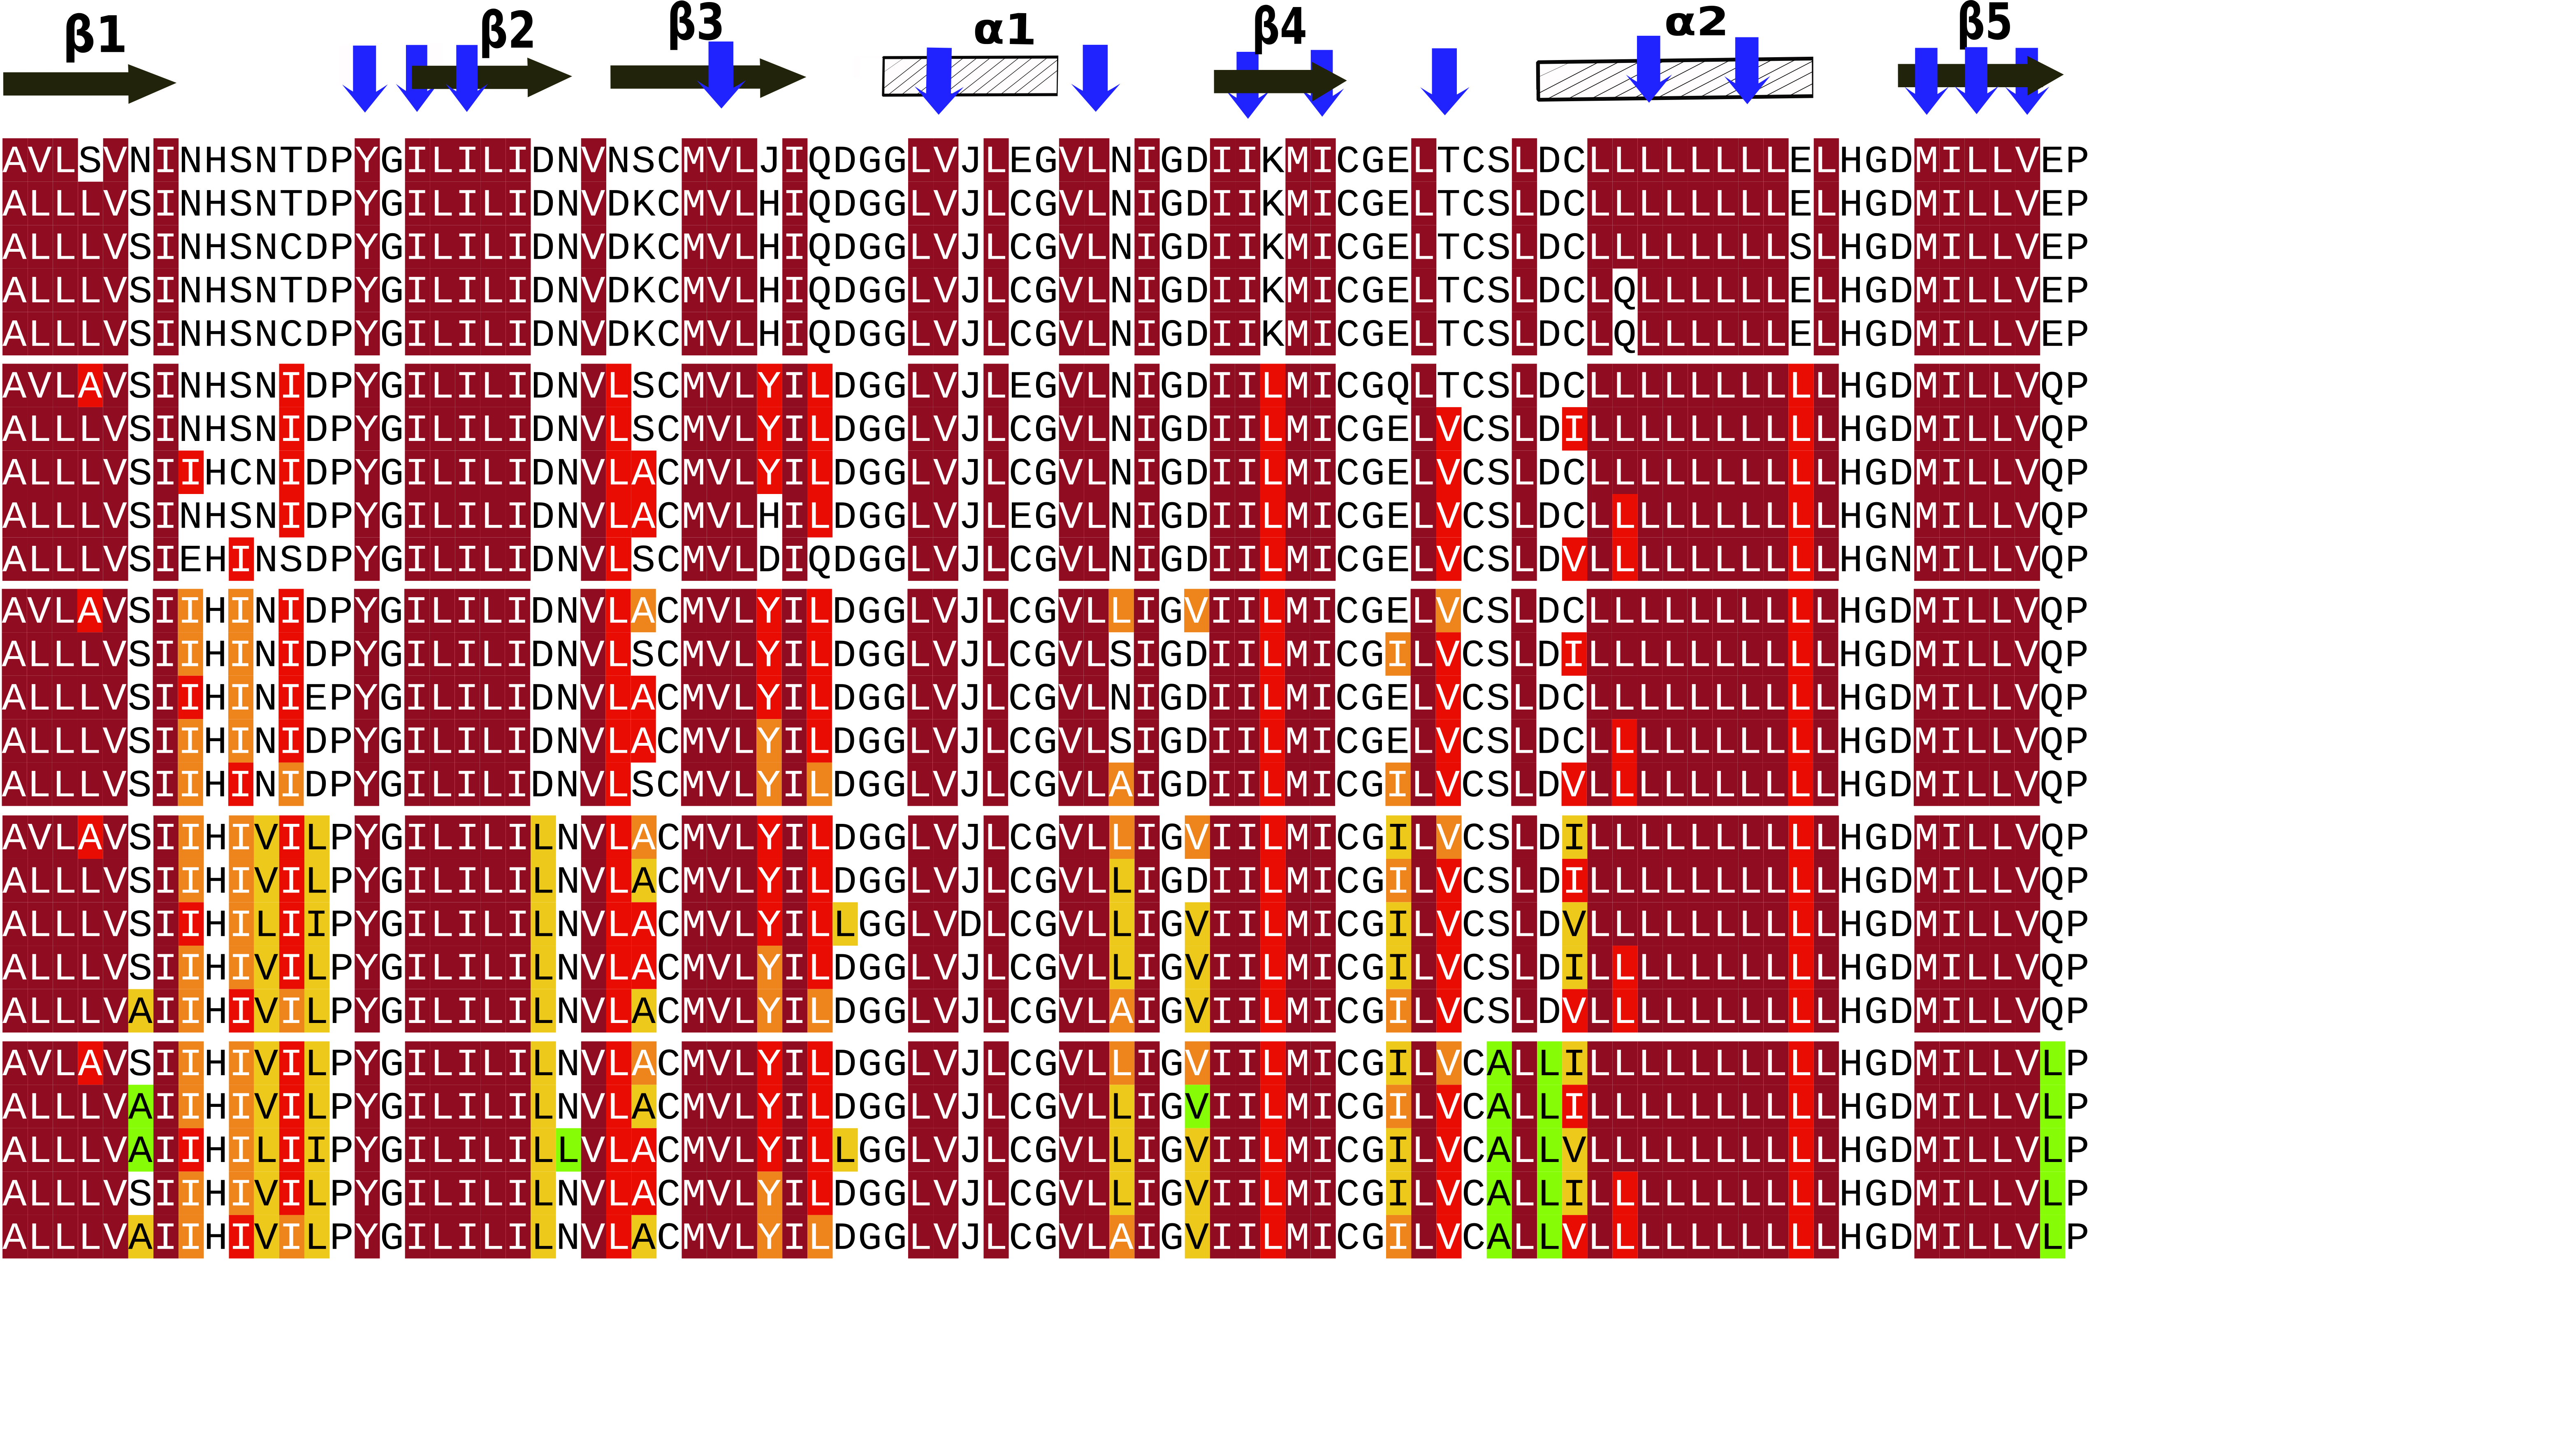
\includegraphics[width=20cm]{boost_hydro/modelA/alignCASK_V2.png} \\
     \end{tabular}
     \caption{Séquences CASK obtenues avec un delta des énergies de références à -0.4,-0.2,0,0.2 et 0.4. Les hydrophobes sont représentés par un dégradé allant du rouge foncé au jaune clair.}
\label{result:PDZ_seed}
   \end{figure}
\end{landscape}

   \clearpage

\begin{landscape}

   \begin{figure}[t]
     \centering
     \begin{tabular}{c}
       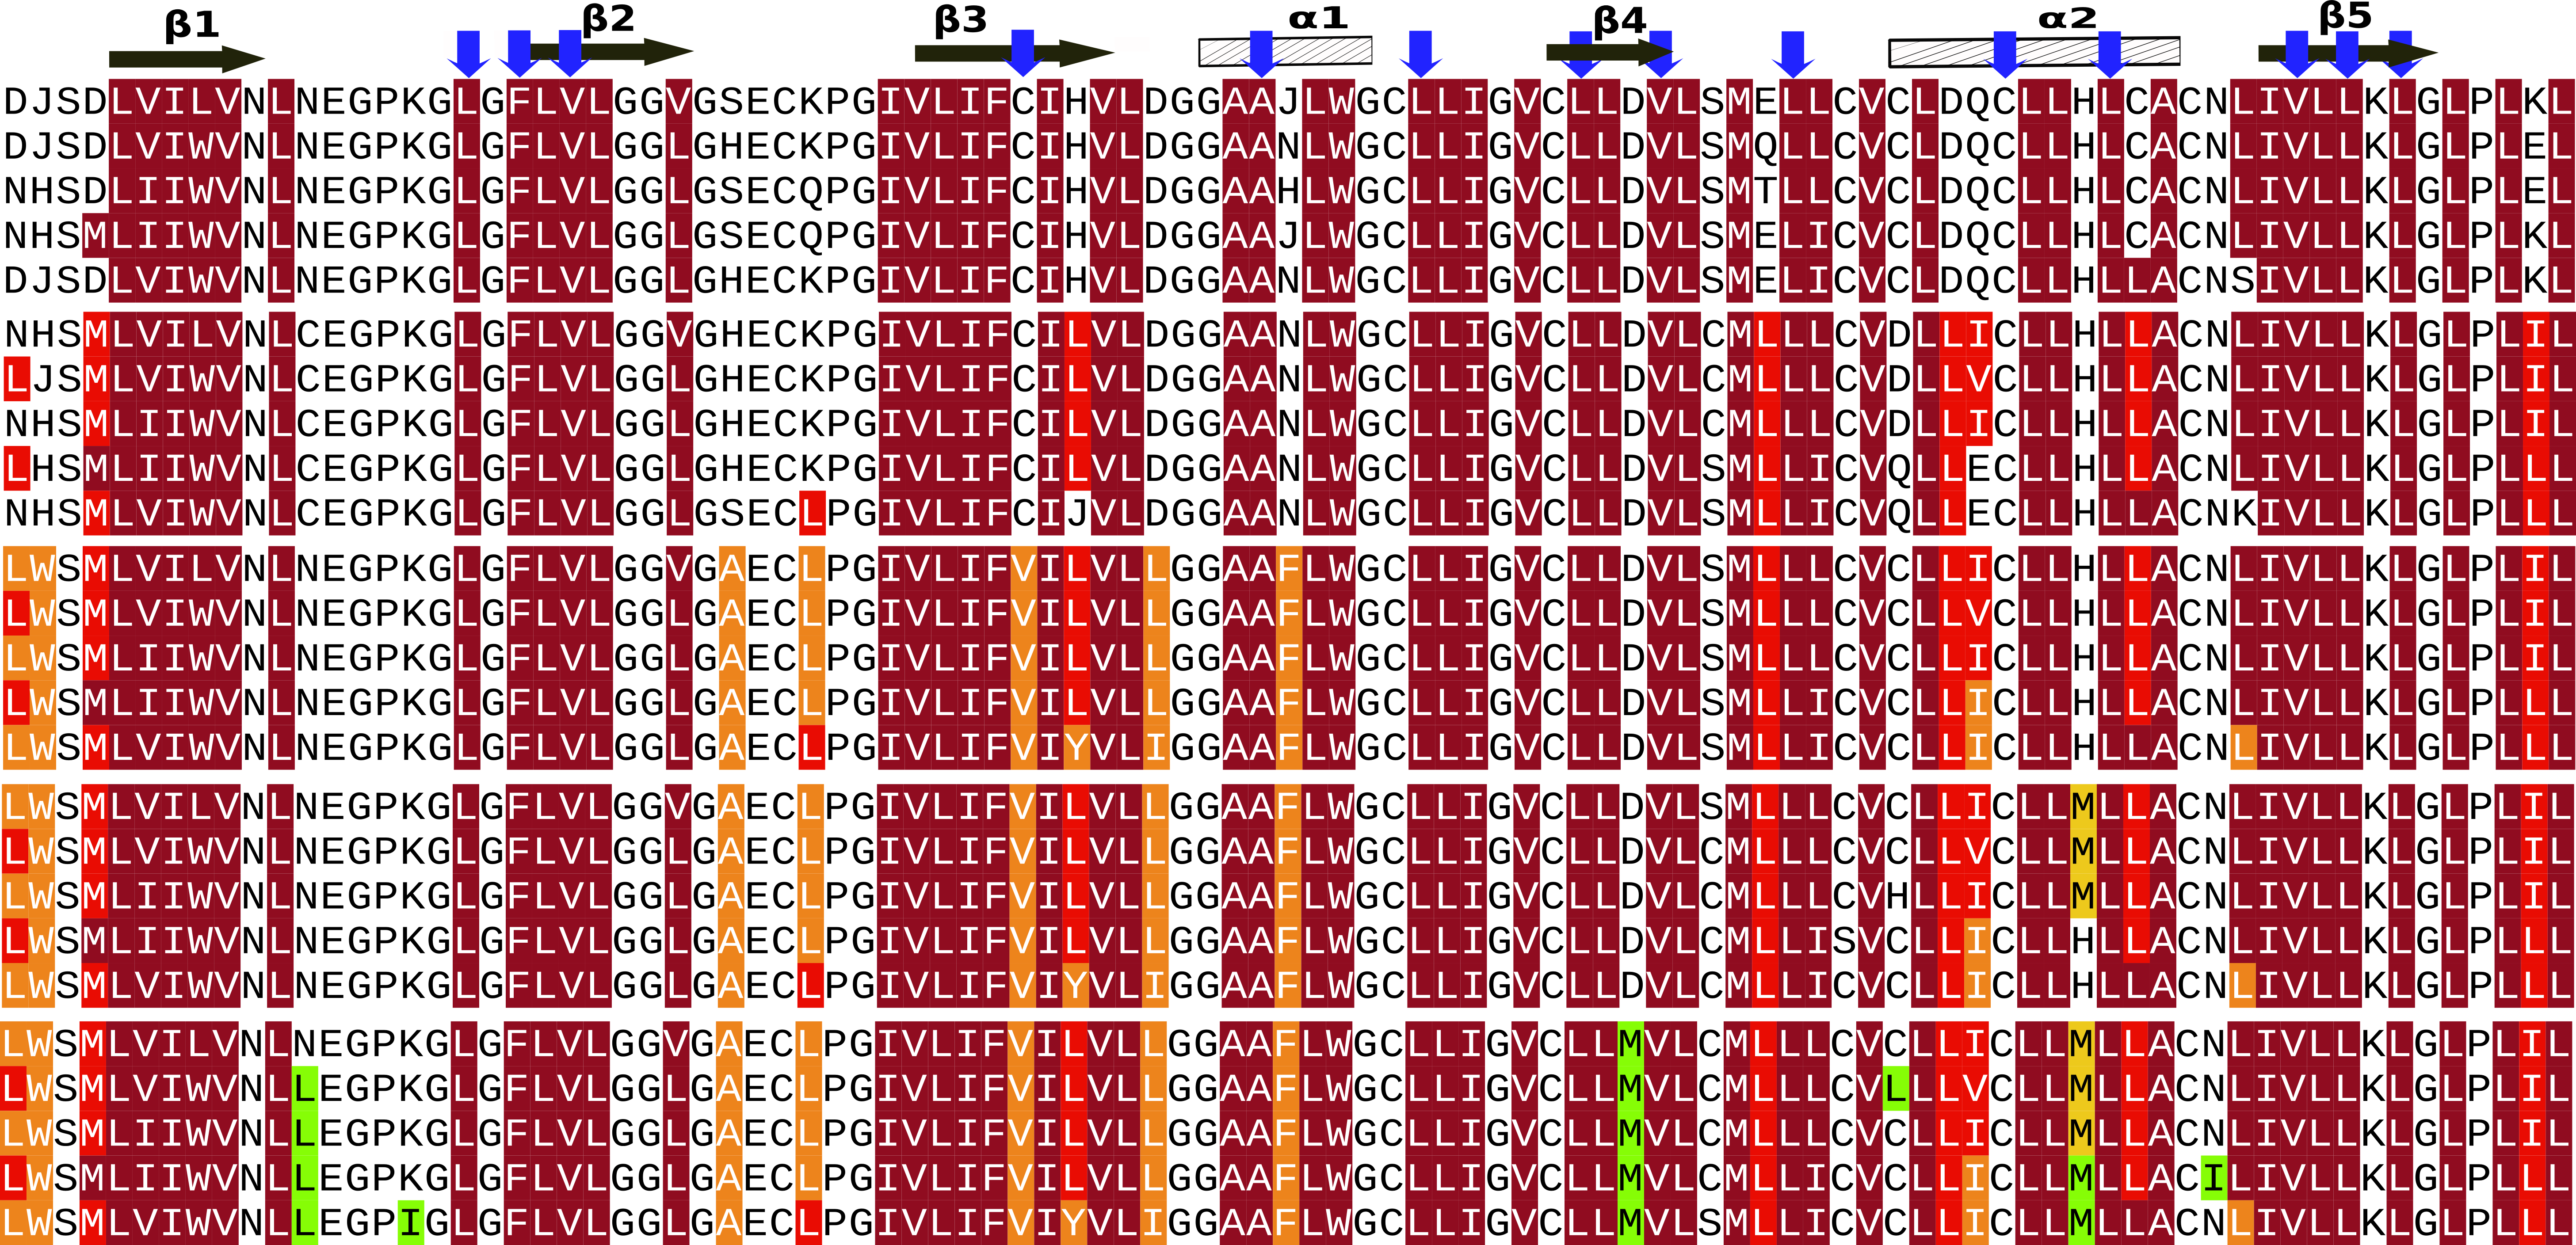
\includegraphics[width=20cm]{boost_hydro/modelA/align2BYG_V2.png} \\
     \end{tabular}
     \caption{Séquences 2BYG obtenues avec un delta des énergies de références à -0.4,-0.2,0,0.2 et 0.4. Les hydrophobes sont représentés par un dégradé allant du rouge foncé au jaune clair.}
\label{result:PDZ_seed}
   \end{figure}
\end{landscape}
   
   \clearpage

   \begin{figure}[t]
     \centering
     \begin{tabular}{c}
       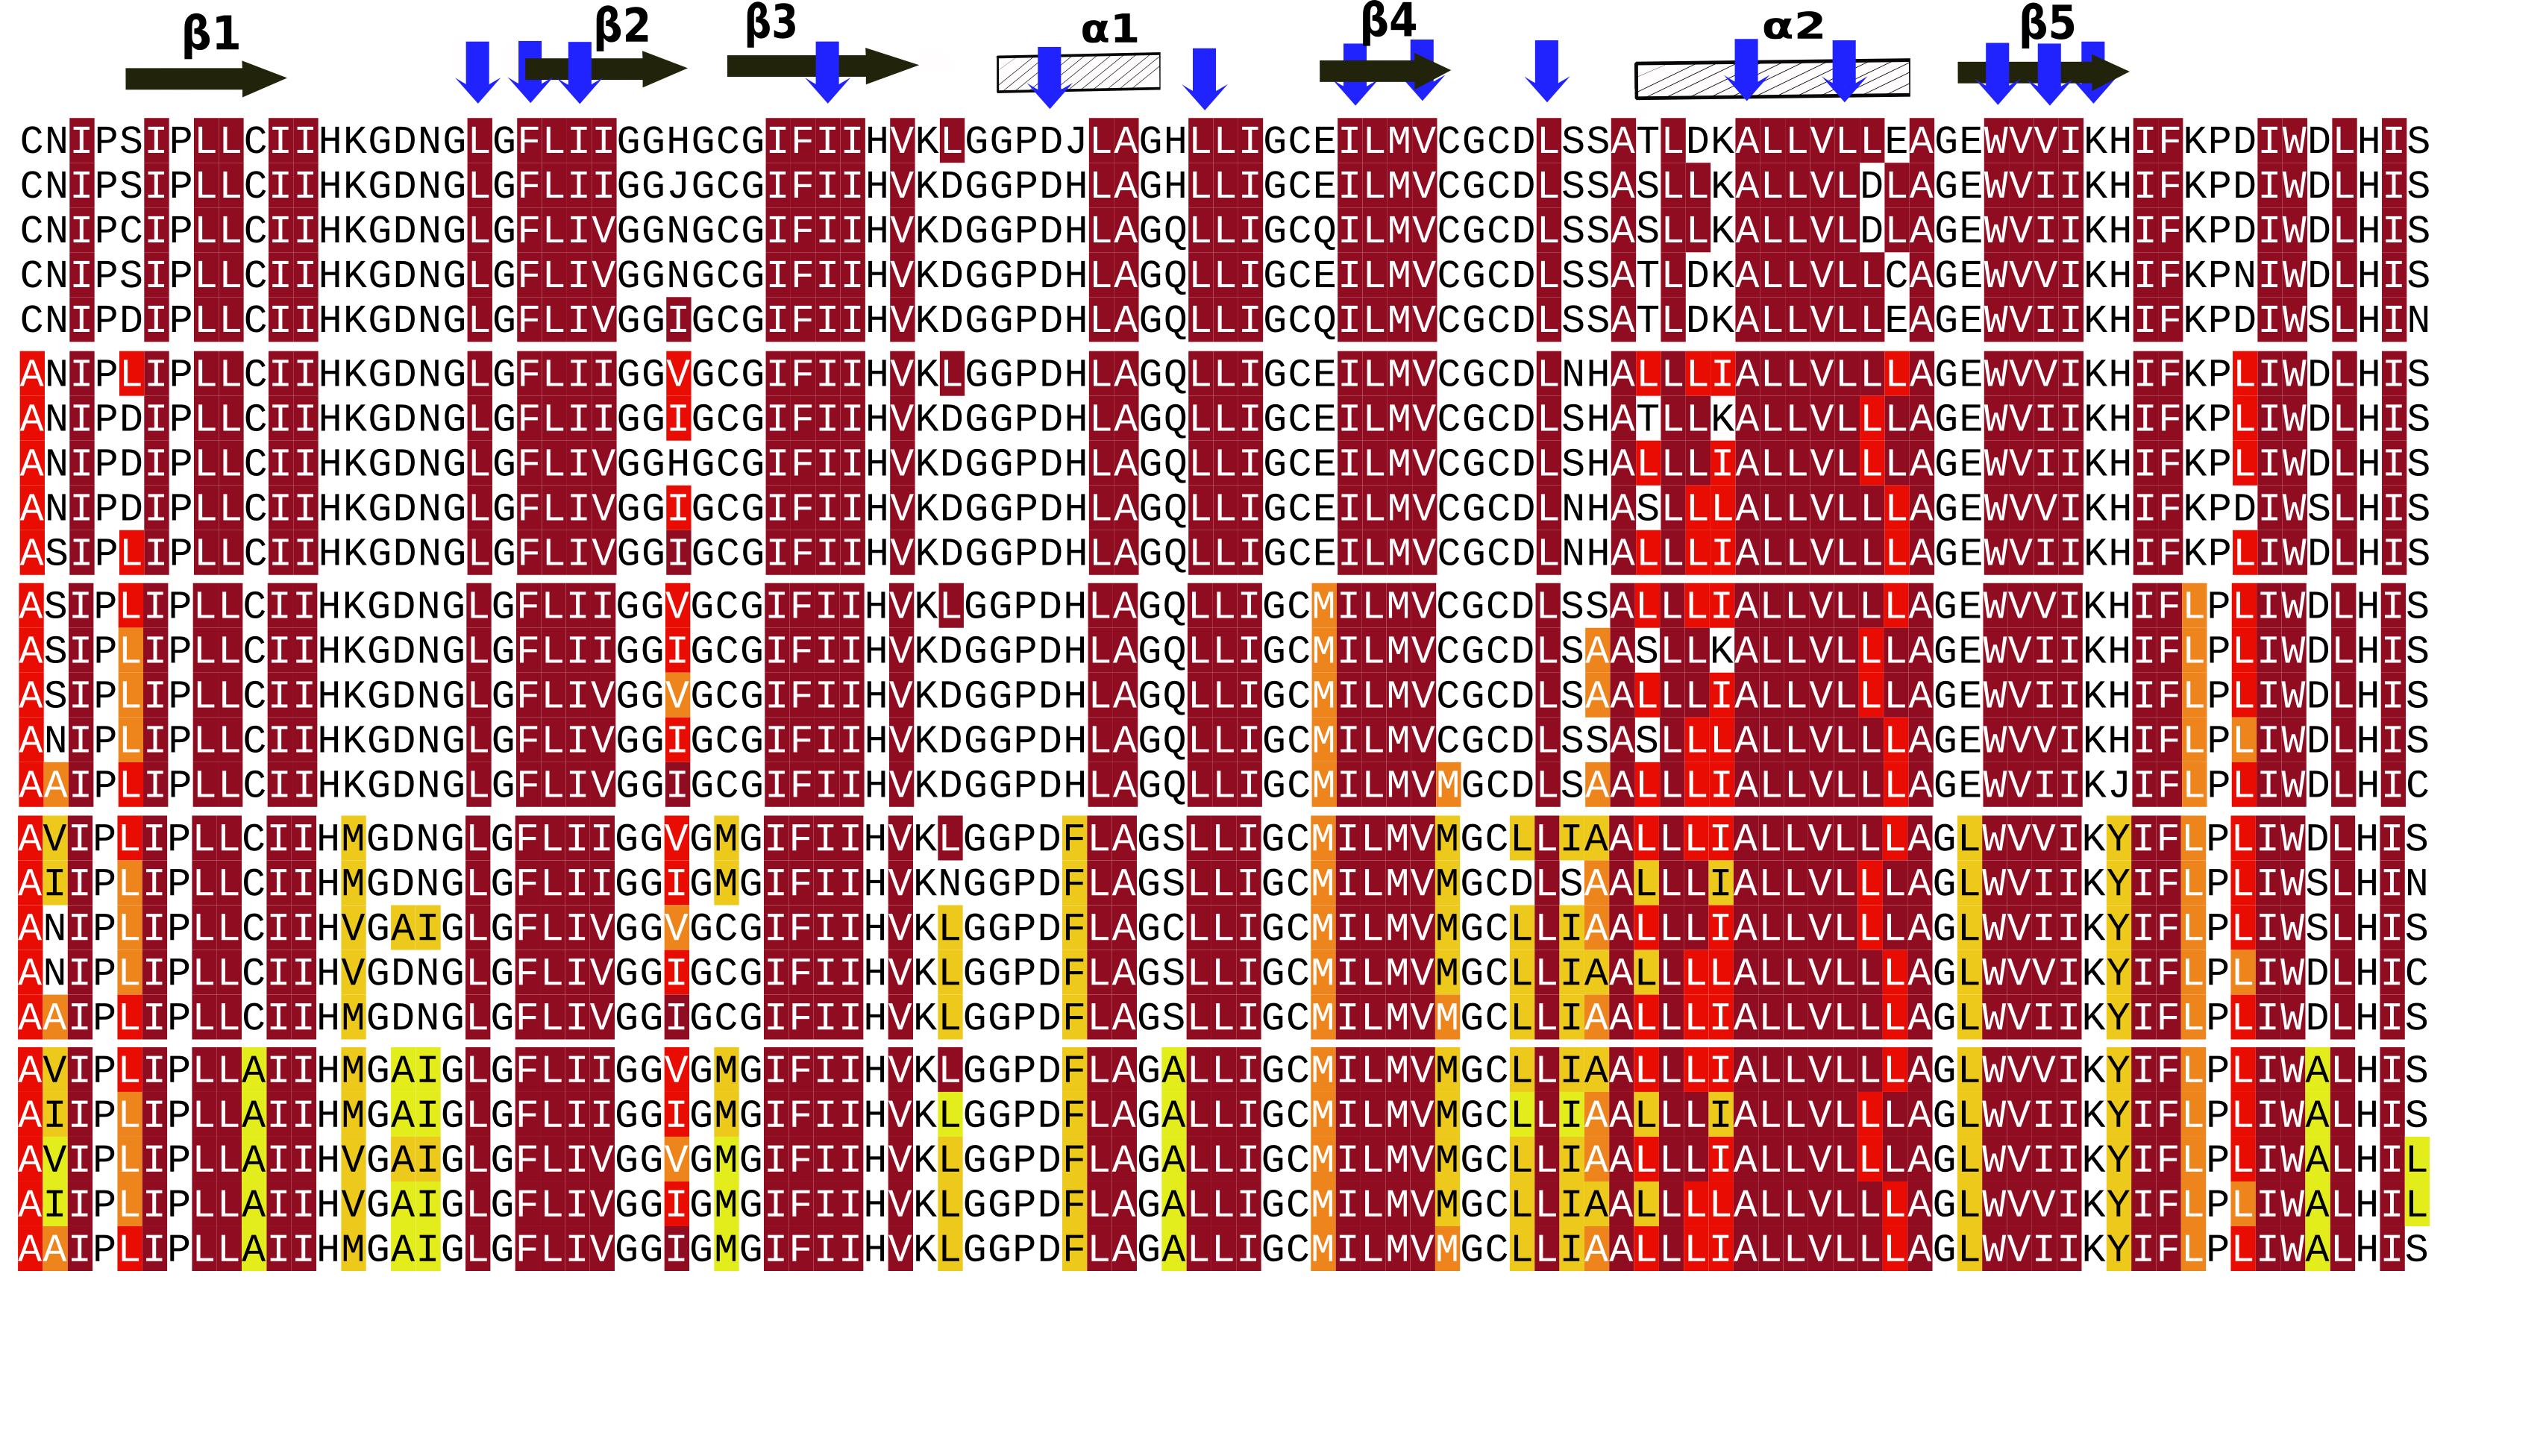
\includegraphics[width=20cm]{boost_hydro/modelA/align3K82.png} \\
     \end{tabular}

     \caption{\small Séquences 3K82 obtenues avec un delta des énergies de références à -0.4,-0.2,0,0.2 et 0.4 .Les hydrophobes pour des deltas de -0.4,-0.2,0,0.2 et 0.4 sont représentés par un dégradé allant du rouge foncé au jaune clair.}

\label{result:PDZ_seed}
   \end{figure}

\end{landscape}


    \clearpage


    \clearpage
    \thispagestyle{empty}
   \begin{figure}[t]
     \centering
     \begin{tabular}{c}
       \includegraphics[width=12cm]{modelB/1R6J_core_simil.png} \\
       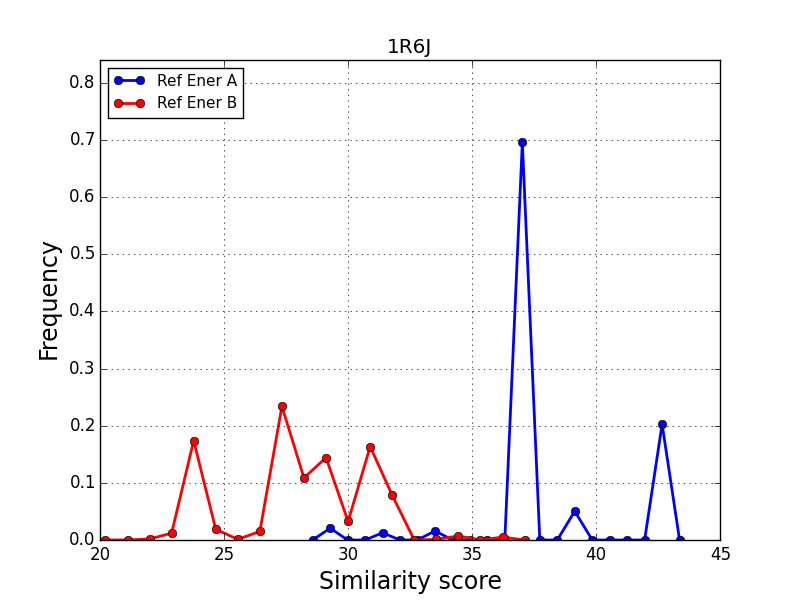
\includegraphics[width=12cm]{modelB/1R6J_simil.png} \\
     \end{tabular}
  \caption{Similarité des séquences 1R6J(modèleB) et Rosetta à l'alignement Pfam RP55,aux positions du cœur (en haut) et sur l'ensemble des positions (en bas).}

\label{graph:Simil_modeB}
   \end{figure}



    \clearpage
    \thispagestyle{empty}
   \begin{figure}[t]
     \centering
     \begin{tabular}{cc}
       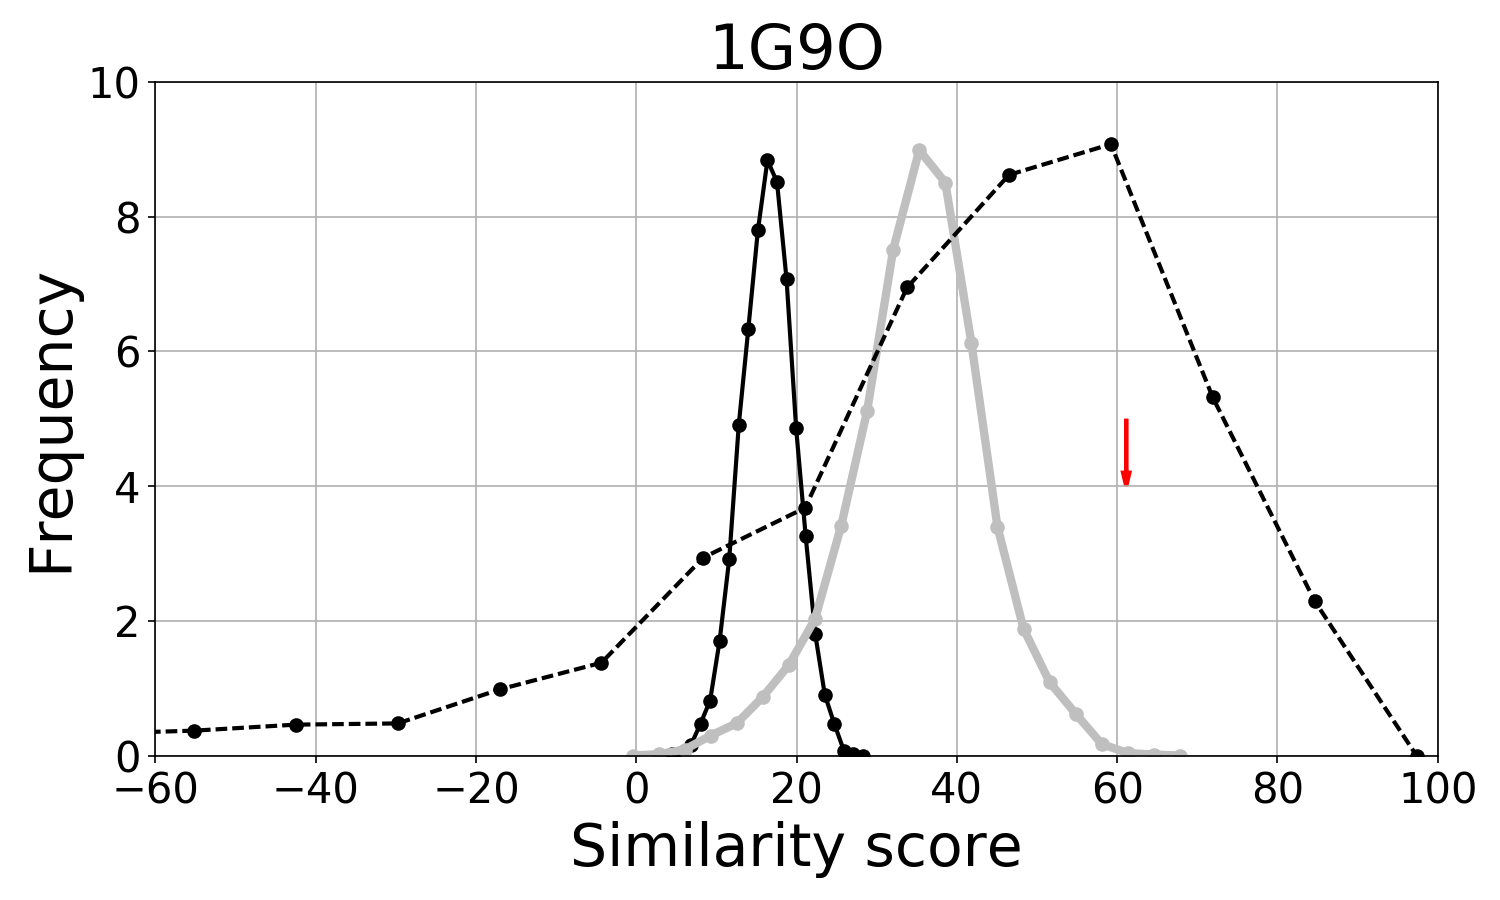
\includegraphics[width=8.4cm]{optGrad0/RP55/1G9O_simil_full.png} &
       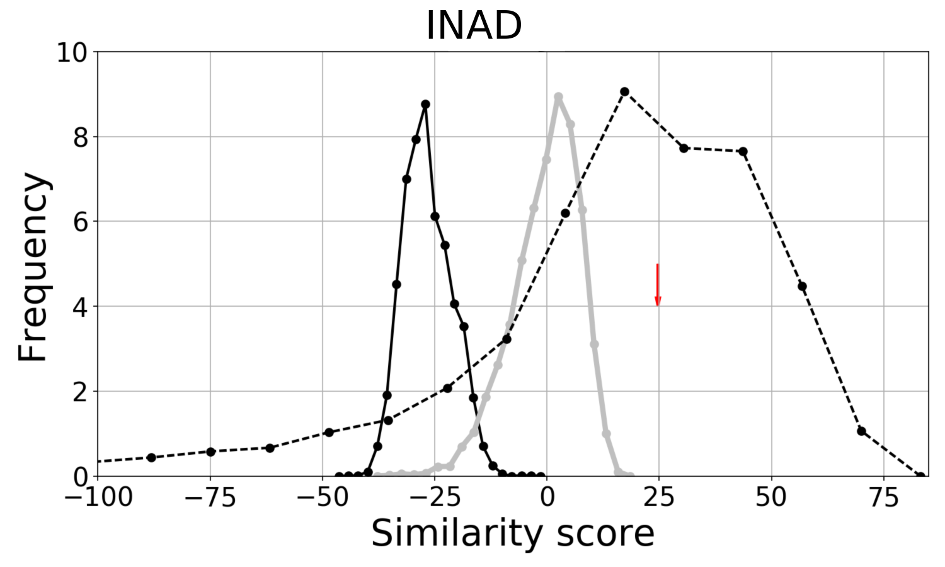
\includegraphics[width=8.4cm]{optGrad0/RP55/1IHJ_simil_full.png} \\
       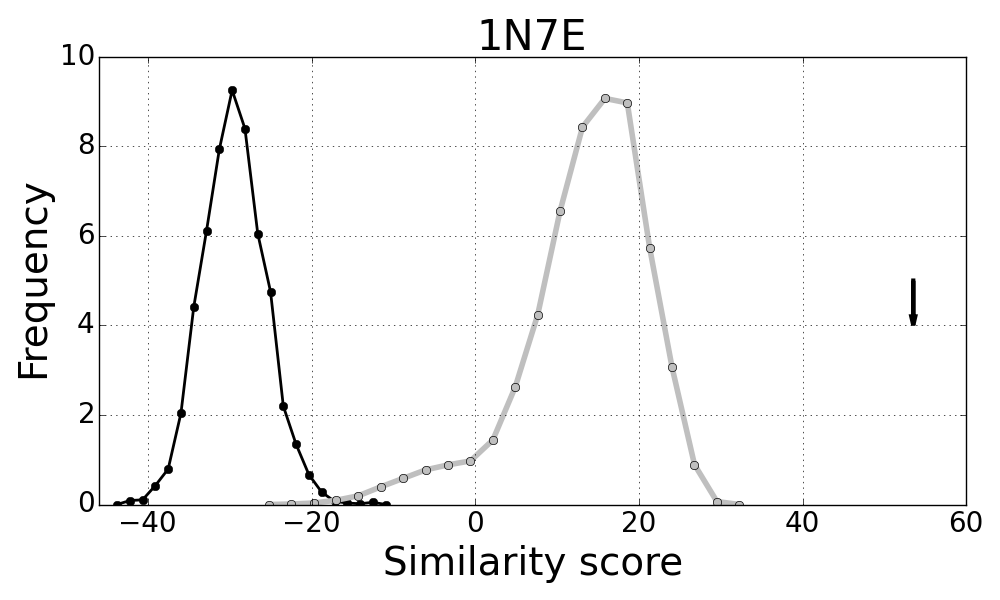
\includegraphics[width=8.4cm]{optGrad0/RP55/1N7E_simil_full.png} &
       \includegraphics[width=8.4cm]{optGrad0/RP55/2BYG_simil_full.png} \\
       \includegraphics[width=8.4cm]{optGrad0/RP55/1R6J_simil_full.png} &
       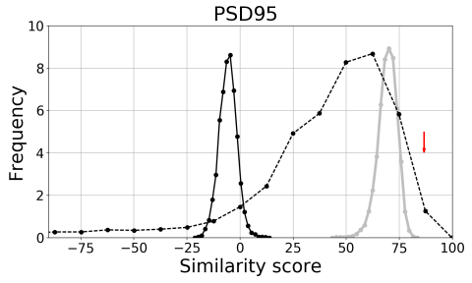
\includegraphics[width=8.4cm]{optGrad0/RP55/3K82_simil_full.png} \\
     \end{tabular}
       \caption{Similarité des séquences Proteus(modèle A) et Rosetta à l'alignement Pfam RP55 sur l'ensemble des positions.}

\label{graph:Simil_Proteus_PDZ_All}
   \end{figure}
   

    \clearpage
    \thispagestyle{empty}
   \begin{figure}[t]
     \centering
     \begin{tabular}{cc} 
       \includegraphics[width=8.4cm]{modelB/1R6J_simil_full.png} &
       \includegraphics[width=8.4cm]{modelB/2BYG_simil_full.png} \\
       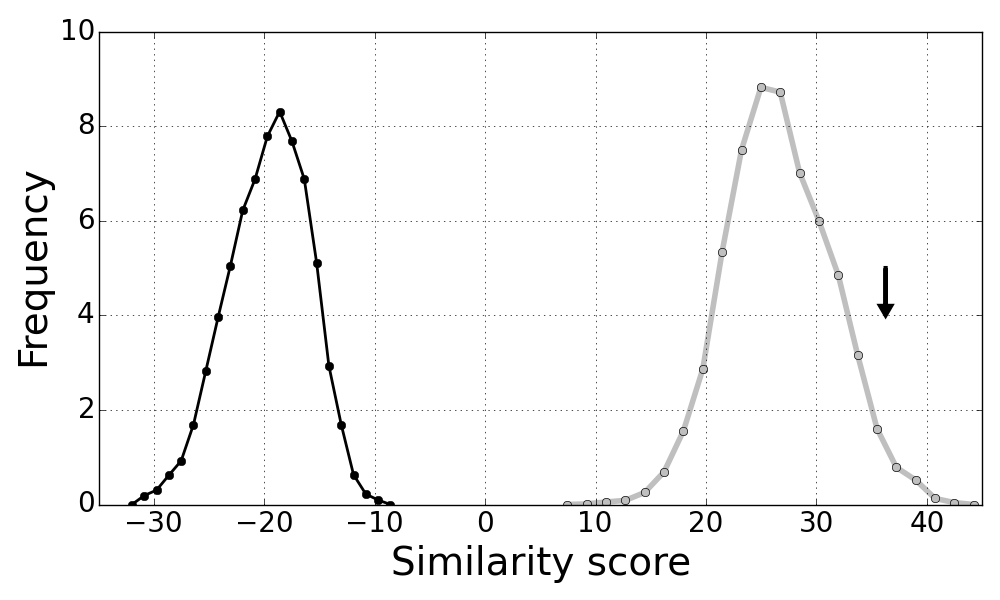
\includegraphics[width=8.4cm]{modelB/1R6J_simil_struct.png} &
       \includegraphics[width=8.4cm]{modelB/2BYG_simil_struct.png} \\
       \includegraphics[width=8.4cm]{modelB/1R6J_simil_core.png} &
       \includegraphics[width=8.4cm]{modelB/2BYG_simil_core.png} \\

     \end{tabular}
  \caption{Similarité des séquences 1R6J et 2BYG produites par proteus modèle B et Rosetta à l'alignement Pfam RP55, sur l'ensemble des positions (au haut),aux positions structurées (au milieu) et sur les positions du coeur (en bas).}

\label{graph:Simil_modeB}
   \end{figure}

    \clearpage
    \thispagestyle{empty}
   \begin{figure}[t]
     \centering
     \begin{tabular}{cc} 
       \includegraphics[width=8.4cm]{modelB/1G9O_simil_full.png} &
       \includegraphics[width=8.4cm]{modelB/1N7E_simil_full.png} \\
       \includegraphics[width=8.4cm]{modelB/1G9O_simil_core.png} &
       \includegraphics[width=8.4cm]{modelB/1N7E_simil_core.png} \\

     \end{tabular}
  \caption{Similarité des séquences 1G9O,1N7E et 3K82 produites par proteus modèle B et Rosetta à l'alignement Pfam RP55, sur l'ensemble des positions (au haut) et sur les positions du coeur (en bas).}

\label{graph:Simil_modeB}
   \end{figure}

   \clearpage   


   
\begin{table}[h]
  \raggedleft{}
  
  \begin{tabular}{cccccc}
    
    \toprule
    Protein & Match/seq & Superfamily & Superfamily & Family & Family \\
            & size      & Evalue      & success     & Evalue & success\\
    \cmidrule{1-6}
    1G9O  & 81/91 & 3.3e-13  & 6656  &  4.0e-3 & 6656 \\
    1IHJ  &  /94 &      &    &   &    \\
    1N7E  & 74/95 & 1.1e-7  & 3754  &  6.9e-3 & 3754 \\
    1R6J  & 67/91 & 6.3e-3  & 6664  &  4.0e-3 & 6664 \\
    2BYG  & 85/97 & 6.0e-9  & 4758  & 5.0e-3  & 4758 \\
    3K82  & /97 &           &   0    &        &  0   \\

    \bottomrule        
  \end{tabular}   
  \caption{Résultats Superfamily pour les séquences Proteus avec le modèle B. --> pas interessant}   
  \label{tab:superfamily}       
\end{table}


   \clearpage   


   
\begin{table}[h]
  \raggedleft{}
  
  \begin{tabular}{cccccc}
    
    \toprule
    Protein & Match/seq & Superfamily & Superfamily & Family & Family \\
            & size      & Evalue      & success     & Evalue & success\\
    \cmidrule{1-6}
    1G9O  & 82/91 & 6.47e-14 & 1000  & 4.70e-3  & 1000 \\
    1IHJ  & 86/94 & 5.93e-11 & 1000  & 2.35e-3  & 1000 \\
    1N7E  & 79/95 & 2.25e-6  & 1000  & 1.16e-2  & 1000 \\
    1R6J  & 62/91 & 9.51e-3  & 9986  & 7.14e-3  & 9986 \\
    2BYG  & 85/97 & 2.98e-9  & 1000  & 4.41e-3  & 1000 \\
    3K82  & 0/97 & 0         &   & 0  &  \\

    \bottomrule        
  \end{tabular}   
  \caption{Résultats Superfamily pour les séquences Proteus avec le modèle B N=6 (convergé au sens des groupes d'aa).}   
  \label{tab:superfamily_model_B6}       
\end{table}


    \clearpage
    \thispagestyle{empty}
   \begin{figure}[t]
     \centering
     \begin{tabular}{cc} 
       \includegraphics[width=8.4cm]{modelB6/1G9O_simil_full.png} &
       \includegraphics[width=8.4cm]{modelB6/1IHJ_simil_full.png} \\
       \includegraphics[width=8.4cm]{modelB6/1R6J_simil_full.png} &
       \includegraphics[width=8.4cm]{modelB6/1N7E_simil_full.png} \\
       \includegraphics[width=8.4cm]{modelB6/2BYG_simil_full.png} &
       \includegraphics[width=8.4cm]{modelB6/3K82_simil_full.png} \\
     \end{tabular}
  \caption{Similarité des séquences des 6 protéines produites par proteus modèle B N=6 (convergé au sens des groupes d'aa) et Rosetta à l'alignement Pfam RP55, sur l'ensemble des positions.}

\label{graph:Simil_modeB}


   \end{figure}



   \begin{table}
     \centering
\caption{La composition en acide aminé (\%) des séquences expérimentales et Proteus après optimisation des énergies de référence. La différence entre expérimentales et Proteus sur les classes est donnée entre crochets.}
\begin{tabular}{l|cccc|cccc}
\hline
\multirow{2}{*}{Res} & \multicolumn{4}{c|}{Experimental n=6}& \multicolumn{4}{c}{Modèle B n=6}\\
 & \multicolumn{2}{c}{Buried} & \multicolumn{2}{c|}{Exposed} & \multicolumn{2}{c}{Buried} & \multicolumn{2}{c}{Exposed} \\
\hline
 & type & classe & type & classe & type & classe & type & classe \\
\hline 
ALA                  & 11.0                 &  \multirow{3}{*}{17.0} & 4.6                  & \multirow{3}{*}{13.4}   &   10.5               & \multirow{2}{*}{11.3}   & 4.4 & \multirow{2}{*}{12.1} \\
CYS                  & 1.3                  &                        & 0.5                  &                         &    0.6               & \multirow{2}{*}{[5.7]}  & 2.3 & \multirow{2}{*}{[1.3]} \\
THR                  & 4.8                  &                        & 8.3                  &                         &    0.2               &                         & 5.4 &                       \\
\hline
\multirow{2}{*}{SER} & \multirow{2}{*}{5.3} & \multirow{2}{*}{5.3}   & \multirow{2}{*}{7.7} & \multirow{2}{*}{7.7}    & \multirow{2}{*}{5.0} &  5.0                    & \multirow{2}{*}{8.1} & 8.1 \\
                     &                      &                        &                      &                         &                      &  [0.3]                  &                      & [-0.4] \\
\hline
ASP                  & 4.3                  & \multirow{2}{*}{6.9}   & 6.0                  & \multirow{2}{*}{17.9}   &   4.4                &  8.5                    & 6.3    & 17.3   \\
GLU                  & 2.6                  &                        & 11.9                 &                         &   4.1                &  [1.4]                  & 11.0   &  [0.6] \\
\hline
ASN                  & 2.6                  & \multirow{2}{*}{4.7}   & 6.7                  & \multirow{2}{*}{12.2}   &   2.0                &  5.6                    & 7.5 & 13.7 \\
GLN                  & 2.1                  &                        & 5.5                  &                         &   3.6                &  [-0.9]                 & 6.2 & [-1.5]    \\
\hline
HIP                  & 1.2                  & \multirow{3}{*}{1.2}   & 5.1                  & \multirow{3}{*}{5.1}    &   1.6                & \multirow{2}{*}{2.2}    & 6.5 & \multirow{2}{*}{8.1} \\
HIE                  & 0.0                  &                        & 0.0                  &                         &   0.3                & \multirow{2}{*}{[-1.0]} & 0.9 & \multirow{2}{*}{[3.0]}  \\
HID                  & 0.0                  &                        & 0.0                  &                         &   0.2                &                         & 0.7 & \\
\hline
ILE                  & 16.0                 & \multirow{3}{*}{50.8}  & 4.2                  & \multirow{3}{*}{14.0}   &   19.3               & \multirow{2}{*}{56.7}   & 5.2 & \multirow{2}{*}{12.4} \\
VAL                  & 16.6                 &                        & 5.4                  &                         &   16.6               & \multirow{2}{*}{[5.9]}  & 4.0 & \multirow{2}{*}{1.6}  \\
LEU                  & 18.2                 &                        & 4.4                  &                         &   20.8               &                         & 3.2 & \\
\hline
\multirow{2}{*}{MET} & \multirow{2}{*}{0.9} & \multirow{2}{*}{0.9}   & \multirow{2}{*}{1.5} & \multirow{2}{*}{1.5}    & \multirow{2}{*}{0.6} & 0.6                    & \multirow{2}{*}{2.3} & 2.3 \\
                     &                      &                        &                      &                         &                      & [0.3]                  &                      & [-0.8] \\
\hline
\multirow{2}{*}{LYS} & \multirow{2}{*}{2.5} & \multirow{2}{*}{2.5}   & \multirow{2}{*}{10.9} & \multirow{2}{*}{10.9}  & \multirow{2}{*}{1.5} &   1.5                   & \multirow{2}{*}{12.9} & 12.9 \\
                     &                      &                        &                       &                        &                      &  [1.0]                  &                       & [2.0] \\
\hline
\multirow{2}{*}{ARG} & \multirow{2}{*}{2.9} & \multirow{2}{*}{2.9}   & \multirow{2}{*}{8.8} & \multirow{2}{*}{8.8}    & \multirow{2}{*}{1.4} & 1.4                    & \multirow{2}{*}{11.4}  & 11.4 \\
                     &                      &                         &                      &                        &                      & [1.5]                  &                        & [-2.6]   \\
\hline
PHE                  & 4.2                  & \multirow{2}{*}{4.2}   & 2.4                  & \multirow{2}{*}{2.4}    &  3.9                 & 4.8                    & 0.4 & 0.7 \\
THP                  & 0.0                  &                        & 0.0                  &                         &  0.9                 & [-0.6]                 & 0.3 & [1.7]               \\
\hline
\multirow{2}{*}{TYR} & \multirow{2}{*}{2.5} & \multirow{2}{*}{2.5}   & \multirow{2}{*}{1.2} & \multirow{2}{*}{1.2}   & \multirow{2}{*}{2.3}  & 2.3                     & \multirow{2}{*}{0.1} & 0.1\\
                     &                      &                        &                      &                         &                      &  [0.2]                  &                      & [1.1]   \\
\hline
GLY                  & 0.1                  & \multirow{2}{*}{0.1}   & 3.1                  & \multirow{2}{*}{4.9}    &   0.0                &  0.0                    & 0.0 & 0.0 \\
PRO                  & 0.0                  &                        & 1.8                  &                         &   0.0                &  [0.1]                  & 0.0 & [4.9]\\
\hline

\end{tabular} 
\end{table}

   \clearpage
\begin{table}[h]
  \raggedleft{}
  
  \begin{tabular}{cccccc}
    
    \toprule
    Protein & Match/seq & Superfamily & Superfamily & Family & Family \\
            & size      & Evalue      & success     & Evalue & success\\
    \cmidrule{1-6}
    1G9O  & 81/91 &  2.00e-12 & 10000  & 9.97e-3 & 10000  \\
    1IHJ  & 84/94 &  4.80e-11 & 10000  & 2.83e-3 & 10000  \\
    1N7E  & 82/95 &  4.73e-8  & 10000  & 5.56e-3 & 10000  \\
    1R6J  & 63/91 &  4.01e-4  &  9999  & 1.05e-2 &  9999  \\
    2BYG  & 84/97 &  3.82e-10 & 10000  & 3.75e-3 & 10000  \\
    3K82  & 46/97 &  7.65e-1  &  5029  & 4.06e-2 &  4719  \\

    \bottomrule        
  \end{tabular}   
  \caption{Résultats Superfamily pour les séquences Proteus avec le modèle B N=6 (E ref optimisées sur 20 cycles selon les classes + 20 cycles selon les types).}   
  \label{tab:superfamily_model_B6}       
\end{table}
   

    \clearpage
    \thispagestyle{empty}
   \begin{figure}[t]
     \centering
     \begin{tabular}{cc} 
       \includegraphics[width=8.4cm]{modelB6+/1G9O_simil_full.png} &
       \includegraphics[width=8.4cm]{modelB6+/1IHJ_simil_full.png} \\
       \includegraphics[width=8.4cm]{modelB6+/1R6J_simil_full.png} &
       \includegraphics[width=8.4cm]{modelB6+/1N7E_simil_full.png} \\
       \includegraphics[width=8.4cm]{modelB6+/2BYG_simil_full.png} &
       \includegraphics[width=8.4cm]{modelB6+/3K82_simil_full.png} \\
     \end{tabular}
  \caption{Similarité des séquences des 6 protéines produites par proteus modèle B N=6 (E ref optimisées sur 20 cycles selon les classes + 20 cycles selon les types) et Rosetta à l'alignement Pfam RP55, sur l'ensemble des positions.}

\label{graph:Simil_modeB6+_core}


   \end{figure}


    \clearpage
    \thispagestyle{empty}
   \begin{figure}[t]
     \centering
     \begin{tabular}{cc} 
       \includegraphics[width=8.4cm]{modelB6+/1G9O_simil_core.png} &
       \includegraphics[width=8.4cm]{modelB6+/1IHJ_simil_core.png} \\
       \includegraphics[width=8.4cm]{modelB6+/1R6J_simil_core.png} &
       \includegraphics[width=8.4cm]{modelB6+/1N7E_simil_core.png} \\
       \includegraphics[width=8.4cm]{modelB6+/2BYG_simil_core.png} &
       \includegraphics[width=8.4cm]{modelB6+/3K82_simil_core.png} \\
     \end{tabular}
  \caption{Similarité des séquences des 6 protéines produites par proteus modèle B N=6 (E ref optimisées sur 20 cycles selon les classes + 20 cycles selon les types) et Rosetta à l'alignement Pfam RP55, sur les positions du coeur.}

\label{graph:Simil_modeB6+_core}


   \end{figure}




    \clearpage
    \thispagestyle{empty}
   \begin{figure}[t]
     \centering
     \begin{tabular}{c} 
       \includegraphics[width=15cm]{modelB6+/3K82_seqlogo.eps} \\

     \end{tabular}
  \caption{Séquences 3K82 modèle B N=6,sur les positions du coeur.}

\label{graph:seqlogo_3K82_core}


   \end{figure}

    \clearpage
    \thispagestyle{empty}
   \begin{figure}[t]
     \centering
     \begin{tabular}{cc} 
       \includegraphics[width=8.4cm]{modelB/1R6J_simil_core.png} &
       \includegraphics[width=8.4cm]{modelB/2BYG_simil_core.png} \\
       \includegraphics[width=8.4cm]{modelB/1R6J_simil_cut.png} &
       \includegraphics[width=8.4cm]{modelB/2BYG_simil_cut.png} \\
     \end{tabular}
  \caption{Similarité des séquences produites par proteus modèle B N=2 et Rosetta à l'alignement Pfam RP55, sur les positions du coeur en haut et sur toutes les positions en bas.}

\label{graph:Simil_modeB2core+cut}


   \end{figure}

   


    \clearpage
    \thispagestyle{empty}
   \begin{figure}[t]
     \centering
     \begin{tabular}{cc} 
       \includegraphics[width=8.4cm]{modelB6+/1R6J_simil_core.png} &
       \includegraphics[width=8.4cm]{modelB6+/2BYG_simil_core.png} \\
       \includegraphics[width=8.4cm]{modelB6+/1R6J_simil_cut.png} &
       \includegraphics[width=8.4cm]{modelB6+/2BYG_simil_cut.png} \\
     \end{tabular}
  \caption{Similarité des séquences produites par proteus modèle B N=6 et Rosetta à l'alignement Pfam RP55, sur les positions du coeur en haut et sur toutes les positions en bas.}

\label{graph:Simil_modeB6core+cut}


   \end{figure}


   

   \clearpage

\begin{landscape}

   \begin{figure}[t]
     \centering
     \begin{tabular}{c}
       \includegraphics[width=20cm]{boost_hydro/modelB2/alignCASK.pdf} \\
     \end{tabular}
     \caption{Séquences CASK modèle B N=2 obtenues avec un delta des énergies de références à -0.4,-0.2,0,0.2 et 0.4. Les hydrophobes sont représentés par un dégradé allant du rouge foncé au jaune clair.}
\label{result:titra_CASK_modelB2}
   \end{figure}
\end{landscape}
   

   \clearpage

\begin{landscape}

   \begin{figure}[t]
     \centering
     \begin{tabular}{c}
       \includegraphics[width=20cm]{boost_hydro/modelB2/alignTiam1.pdf} \\
     \end{tabular}
     \caption{Séquences Tiam1 modèle B N=2 obtenues avec un delta des énergies de références à -0.4,-0.2,0,0.2 et 0.4. Les hydrophobes sont représentés par un dégradé allant du rouge foncé au jaune clair.}
\label{result:titra_Tiam1_modelB2}
   \end{figure}
\end{landscape}


    \clearpage
    \thispagestyle{empty}
   \begin{figure}[t]
     \centering
     \begin{tabular}{cc} 
       \includegraphics[width=8.4cm]{modelExactGB/1G9O_simil_cut.png} &
       \includegraphics[width=8.4cm]{modelExactGB/1R6J_simil_cut.png} \\
       \includegraphics[width=8.4cm]{modelExactGB/1G9O_simil_core.png} &
       \includegraphics[width=8.4cm]{modelExactGB/1R6J_simil_core.png} \\
     \end{tabular}
  \caption{Similarité des séquences produites par proteus modèle exactGB  (E ref optimisées sur 20 cycles selon les classes + 20 cycles selon les types) et Rosetta à l'alignement Pfam RP55, sur toutes les postions en haut  et sur les positions du coeur en bas.}

\label{graph:Simil_modelExactGB}


   \end{figure}



   \clearpage
\begin{table}[h]
  \raggedleft{}
  
  \begin{tabular}{cccccc}
    
    \toprule
    Protein & Match/seq & Superfamily & Superfamily & Family & Family \\
            & size      & Evalue      & success     & Evalue & success\\
    \cmidrule{1-6}
    1G9O  & 79/91 & 9.23e-12  & 10000  & 9.17e-3 & 10000  \\
    1R6J  & 75/91 &  3.05e-3  &  9991  & 4.04e-3 &  9991  \\
    2BYG  & /97   &           &        &         &        \\

    \bottomrule        
  \end{tabular}   
  \caption{Résultats Superfamily pour les séquences Proteus avec le modèle exactGB (E ref optimisées sur 20 cycles selon les classes + 20 cycles selon les types).}   
  \label{tab:superfamily_model_B6}       
\end{table}

   
   
   

%%% Local Variables:
%%% mode: latex
%%% TeX-master: "../../rapport"
%%% End:

\clearplaindoublepage{}
\chapter{PDZ}
\label{chap:PDZ}

Nous cherchons maintenant à évaluer les performances de notre modèle CPD sur un ensemble de protéines de la famille PDZ. Nous utilisons les résultats précédents, en particulier ceux de la section ??, pour définir les valeurs des paramètres de l'optimisation du Monte-Carlo.  Ici, nous allons confronter nos résultats à ceux  du fameux outils de Rosetta obtenue dans des conditions identiques. Comme dans les situations précédentes le backbone de nos protéines est fixé tout le long de l'étude.La fonctions d'énergie est calculée en utilisant le model MM/GBSA (voir ?? et la chapitre 1 pour les détails).Mais ici, nous reprenons l'optimisation des énergies de référence pour d'adapter à l'ensemble des protéines PDZ.


\section{L'ensemble des protéines PDZ} 

Nous sélectionnons huit protéines de la famille PDZ, avec les trois présentes dans l'ensemble étudié au chapitre précédent: 1G9O,1R6J et 2BYG, aux quelles sont ajoutés 1IHJ, 1N7E, 3K82 et Cask , tiam1 représenté par .... et ... dans la base de données PDB. Cela constitue un ensemble où le nombre de positions actives , c'est à dire les postions qui vont être muté , est du même ordre pour chaque séquence d'acide aminé des protéines ( voir le tableau \ref{tab:protéines_PDZ}).

\paragraph{}
Pour caractériser les homologies dans cet ensemble, une série de requête blast est effectuée sur chaque paire de séquences en utilisant le programme blastp.Il apparaît que 1R6J et TiAM1 sont atypiques dans l'ensemble avec , aucun homologue avec une E-value inférieure à 1e-7 et plusieurs E-value supérieur à 10. 3K82 est la protéine plus consensuelle , ayant d'une part une homologie avec toutes les autres à au plus 6e-04 , et d'autre part ayant 4 homologues à moins de 2e-10, pour pourcentage d'identité compris entre 30 et 46.Globalement, il n'y a que peu d'homologies, la plus forte n'étant que de 3e-15 entre 3K82 et 2BYG pour un pourcentage d'identité de 37. Les détails sont dans le tableau \ref{tab:Xblast}.

\label{sec:ensemble_PDZ}

    \begin{table}[!htbp]
      \centering

      \begin{tabular}{ccc}

        \toprule
        Code PDB & résidus & nombre de positions actives\\
        \cmidrule{1-3}
        1G9O  & 	9-99	 & 	76	 \\
        1IHJ  & 	13-105	 & 	82	 \\
        1N7E  & 	668-761	 & 	79	 \\
        1R6J  & 	193-273	 & 	72	 \\
        2BYG  & 	186-282	 & 	82	 \\
        3K82  & 	305-402	 & 	80	 \\
        Cask  & 	487-568	 & 	74	 \\
        Tiam1 & 	838-930	 & 	84	 \\
        \bottomrule

      \end{tabular}      
      \caption{Les protéines PDZ}
\label{tab:protéines_PDZ}      
    \end{table}

\paragraph{Alignements Blast croisés}

\clearpage
    \begin{table}[!htbp]
        \raggedleft{}
\scalebox{0.75}{
      \begin{tabular}{ccccccccc}

        \toprule
        Protein & 1G9O        & 1IHJ      & 1N7E        & 1R6J        & 2BYG       & 3K82       & CASK       & TIAM1 \\
        \cmidrule{1-9}

        1G9O    & 2e-66 (100)& 5e-10 (40) & 0.002 (25)  & 3e-07 (25)  & 2e-11 (35) & 1e-12 (30) & 5e-05 (25) & 9e-07(35)\\     
        1IHJ    & 5e-10 (40) & 3e-68 (100)&  2e-07 (27) & [18]        & 2e-08 (27) & 9e-14 (46) & 4e-06 (35) & [16]    \\
        1N7E    & 0.002 (25) & 2e-07 (27) &  3e-67 (100)& [21]        & 3e-14 (36) & 2e-10 (37) & 9e-12 (30) & 5e-05 (35)\\
        1R6J    & 3e-07 (25) & [18]       &    [21]     & 1e-59 (100) &  [17]      & 1e-06 (32) & 0.007 (32) & [18]    \\
        2BYG    & 2e-11 (35) & 2e-08 (27) &  3e-14 (37) & [17]        & 7e-71 (100)& 3e-15 (37) & 2e-07 (28) & 5e-05 (41)\\
        3K82    & 1e-12 (30) & 9e-14 (46) &  2e-10 (36) & 1e-06 (32)  & 3e-15 (37) & 4e-70 (100)& 1e-07 (27) & 6e-04(33) \\
        Cask    & 5e-05 (25) & 4e-06 (35) &  9e-12 (30) & 0.007 (32)  & 2e-07 (28) & 1e-07 (27) & 7e-61 (100)& 5e-04(33) \\
        Tiam1   & 9e-07 (35) &  [16]      &  5e-05 (35) & [18]        & 5e-05 (41) & 6e-04 (33) & 5e-04 (33) & 1e-68 (100)\\
        \bottomrule


      \end{tabular} 
}     
      \caption{E-value et pourcentage d'identité des alignements Blast native versus native pour nos séquences PDZ.S'il n'y a pas de touche avec une E-value inférieure à 10,[] donne le pourcentage d'identité du couple dans l'alignement des 6 séquences sauvages.}
\label{tab:Xblast}      
    \end{table}
    \clearpage



\paragraph{similarité des homologues}

\clearpage
    \begin{table}[!htbp]
        \raggedleft{}
\scalebox{0.75}{
      \begin{tabular}{ccccccccc}

        \toprule
        Protein & 1G9O        & 1IHJ      & 1N7E        & 1R6J        & 2BYG       & 3K82       & CASK       & TIAM1 \\
        \cmidrule{1-9}

        1G9O    & 326 &  64 &  15 &  15 &  59 & 112 & 49  &   1  \\     
        1IHJ    &  64 & 221 &  56 &  -9 &  88 & 107 & 25  &   9  \\
        1N7E    &  15 &  56 & 378 &  24 &  65 &  87 & 90  &  39  \\
        1R6J    &  15 & -10 &  24 & 311 & -26 &  22 & 42  & -18  \\
        2BYG    &  59 &  88 &  65 & -26 & 325 & 110 & 24  &  22  \\
        3K82    & 112 & 107 &  87 &  22 & 110 & 325 & 66  &  21  \\
        Cask    &  49 &  25 &  90 &  42 &  23 &  66 & 308 & 37   \\
        Tiam1   &  1  &  10 &  39 & -18 &  22 &  21 & 37  & 371 \\
        \bottomrule


      \end{tabular} 
}     
      \caption{Similarité des séquences expérimentales homologues, pour les 8 protéines PDZ.}
\label{tab:XSIMIL}      
    \end{table}
    \clearpage


\subsection{Description}

\subsection{Requêtes Blast croisées}

\subsection{L'alignement choisi}

\subsection{Le cœur PDZ sélectionné}


\section{L'optimisation des énergies de référence} 
\label{sec:optERef}

Dans notre système CPD, l'état replié joue un rôle important parce que les séquences d’intérêts sont celles obtenues en minimisant la différentes d’énergie entre l'état déplié et l'état replié. Donc c'est très important!.
Mais l'état déplié, lui est représenté comme une chaîne polypeptidique largement étendue, de telle façon que nous considérons que chaque résidu X interagie uniquement avec le backbone environnent et avec le solvant.Puis, ce modèle est ajuster empiriquement en comparant les populations de chaque type de résidu dans les séquences calculées avec les populations dans les séquences expérimentales.L'optimisation des énergies de référence consiste alors à corriger ces énergies de telles façons que la populations pour un type aa donné dans les séquences calculés coïncidence avec la population expérimentale de ce type. Il s'agit alors d'un problème de convergence pour la suite d'itérer de proteus + ajustement.

\subsection{La composition naturelle en acide aminé}

Pour avoir une composition naturelle en acide aminé de nos protéines,nous sélectionnons un ensemble de séquences homologues pour chacunes de nos 8 protéines.Pour cela, sur le site Web d'Uniprot (http://www.uniprot.org/ ), nous effectuons des requêtes sur la base de données ``siwwprot + trEmBL'' avec la matrice BLOSUM62 sans l'option \og filtre\fg et avec l'option \og Gapped\fg. Nous obtenons un premier ensemble pour chaque cas en se limitant aux homologues de bonnes qualité au regard de E-value et du pourcentage d'identité , tout en conservant  en même temps une certaine diversité.Cela oblige pour certaines protéine à accepter des E-values plus haute que  1e-40, notamment 1IHJ et 1G9O , respectivement 1e-32 et 1e-10 ,pour avoir un nombre d'homologue suffisant.Ensuite, les redondances les plus flagrantes sont enlevées manuellement.Finalement,les ensembles se composent de 42 à 126 homologues,avec des pourcentages d'identité supérieurs à 66 \% excepté pour 1IHJ où il a fallut descendre jusqu'à 38\% d'identité.Voir le tableau pour les détails \ref{tab:select_homo}.


    \clearpage


    \begin{table}[!htbp]
      \centering

      \begin{tabular}{ccc}

        \toprule
        Code PDB & résidus & nombre de positions actives\\
        \cmidrule{1-3}
        1G9O  & 	9-99	 & 	76	 \\
        1IHJ  & 	12-105	 & 	82	 \\
        1N7E  & 	667-761	 & 	79	 \\
        1R6J  & 	192-273	 & 	72	 \\
        2BYG  & 	186-282	 & 	82	 \\
        3K82  & 	305-402	 & 	80	 \\
        Cask  & 	487-568	 & 	74	 \\
        Tiam1 & 	838-930	 & 	84	 \\
        \bottomrule

      \end{tabular}      
      \caption{Les protéines PDZ}
\label{tab:protéines_PDZ}      
    \end{table}



requête sur le site d'uniprot

Target database uniprot (swissprot + trEMBL)

Matrix BLOSUM62

Filtering NO

Gapped YES


Puis selection à la main -->
enveler les redondances flagrantes
 + avoir un compromis entre diversité et qualité de l'alignement
 + rester dans la zone de ce qui a déjà été fait.

On coupe le début et/ou la fin (10-20 \%)



    \begin{table}[!htbp]
      \centering

      \begin{tabular}{cccc}

        \toprule
        protéines & \% identité \\
        \cmidrule{1-4}
     1G9O  & 62  &    1e-32  &  67-95 \\
     1IHJ  & 42  &    1e-10  &  38-95 \\
     1N7E  & 48  &    1e-45  &  84-95 \\
     1R6J  & 85  &    1e-43  &  85-95 \\
     2BYG  & 43  &    1e-41  &  78-95 \\
     3K82  & 50  &    1e-46  &  81-95 \\
     Cask  & 126 &    7e-28  &  60-85 \\
     Tiam1 & 50  &    2e-23  &  60-85 \\

        \bottomrule

      \end{tabular}      
      \caption{Sélection des homologues.}
\label{tab:select_homo}      
    \end{table}

    \clearpage


\subsection{Première méthode}

Le modèle de l'état déplié considère qu'un résidu X n’interagit pas avec ses résidus voisins, donc l'énergie de l'état déplié de la chaîne polypeptidique peut s'écrire comme la somme sur les résidus des énergies de référence.Ces énergies sont dans un premier temps déterminées par une simple modélisation en peptide étendu.
 Nous souhaitons améliorer les énergies de référence par une correction empirique. Cette correction a pour objectif de permettre à proteus de produire des populations d'acides aminés comparables à celles observées dans la composition naturelle définie au paragraphe précédent.
Notons $C_x$ cette correction à l'énergie initiale $E_X^{ini}$ pour le résidu X.




\subsection{Seconde méthode d'itération}

\section{Résultats} 



    \clearpage

   \begin{figure}[t]
     \centering
     \begin{tabular}{c}
       \includegraphics[width=17cm]{align/1G9O.png} \\
     \end{tabular}
     \caption{L'alignement 1G9O }
\label{graph:convEref}
   \end{figure}

    \clearpage

   \begin{figure}[t]
     \centering
     \begin{tabular}{c}
       \includegraphics[width=17cm]{align/1IHJ.png} \\
     \end{tabular}
     \caption{L'alignement 1IHJ }
\label{graph:convEref}
   \end{figure}

    \clearpage

   \begin{figure}[t]
     \centering
     \begin{tabular}{c}
       \includegraphics[width=17cm]{align/1N7E.png} \\
     \end{tabular}
     \caption{L'alignement 1N7E }
\label{graph:convEref}
   \end{figure}

    \clearpage

   \begin{figure}[t]
     \centering
     \begin{tabular}{c}
       \includegraphics[width=17cm]{align/1R6J.png} \\
     \end{tabular}
     \caption{L'alignement 1R6J }
\label{graph:convEref}
   \end{figure}

    \clearpage

   \begin{figure}[t]
     \centering
     \begin{tabular}{c}
       \includegraphics[width=17cm]{align/2BYG.png} \\
     \end{tabular}
     \caption{L'alignement 2BYG }
\label{graph:convEref}
   \end{figure}

    \clearpage

   \begin{figure}[t]
     \centering
     \begin{tabular}{c}
       \includegraphics[width=17cm]{align/3K82.png} \\
     \end{tabular}
     \caption{L'alignement 3K82 }
\label{graph:convEref}
   \end{figure}

    \clearpage




\paragraph{Fréquences des acides aminés}


    \begin{table}[!htbp]
      \centering

      \begin{tabular}{ccc}

        \toprule
        Groupe & acides aminés & propriétés\\
        \cmidrule{1-3}

        1   & Ala,Cys,Thr & petit\\
        2   & Ser &\\
        \cmidrule{1-3}
        3   & Glu,Asp & chargé négativement\\
        \cmidrule{1-3}
        4   & Gln,Asn & polaire\\
        \cmidrule{1-3}
        5   & Ile,Leu,Val & apolaire\\
        \cmidrule{1-3}
        6   & Met & non polaire\\
        \cmidrule{1-3}
        7   & Hip,Hid,Hie & chargé positivement\\
        8   & Arg \\
        9   & Lys \\
        \cmidrule{1-3}
        10  & Phe,Trp & aromatique\\
        11  & Tyr \\
        \cmidrule{1-3}
        12  & Gly,Pro & non mutable\\
        \bottomrule


      \end{tabular}      
      \caption{Les groupes d'acides aminés utilisés pour l'optimisation des énergies de référence.}
\label{tab:AA_groupes}      
    \end{table}



    \begin{table}[!htbp]
      \centering

      \begin{tabular}{cc}

        \toprule
        acides aminés & fréquence \\
        \cmidrule{1-2}

        Ala &   0.090 \\      
        Cys &   0.028 \\  
        Thr &   0.060 \\  
        Ser &   0.071 \\  
        Glu &   0.062 \\  
        Asp &   0.044 \\  
        Gln &   0.039 \\  
        Asn &   0.055 \\  
        Ile &   0.046 \\  
        Leu &   0.075 \\  
        Val &   0.069 \\  
        Met &   0.017 \\  
        His &   0.021 \\  
        Arg &   0.047 \\  
        Lys &   0.070 \\  
        Phe &   0.035 \\  
        Trp &   0.011 \\  
        Tyr &   0.035 \\  
        Gly &   0.075 \\  
        Pro &   0.046 \\      
        \bottomrule


      \end{tabular}      
      \caption{Fréquences des acides aminés d'après dans les  protéines.}
\label{tab:AA_groupes}      
    \end{table}


    \begin{table}[!htbp]
      \centering

      \begin{tabular}{c|cc|cc}

        \toprule
        acides aminés & résidus enfouis & groupe & résidus exposés & groupe\\
        \cmidrule{1-5}

        Ala &         0.068 &       &   0.048   \\
        Cys &         0.016 &  0.147  &   0.004 & 0.135  \\    
        Thr &         0.062 &        &   0.081   \\
        \cmidrule{1-5}
        Ser &        \multicolumn{2}{c|}{0.067}     &   \multicolumn{2}{c}{0.066}  \\
        \cmidrule{1-5}
        Glu &         0.053 & 0.089        &   0.078 & 0.134 \\
        Asp &         0.035 &    &   0.055   \\
        \cmidrule{1-5}
        Gln &         0.022 & 0.051 &   0.052 & 0.117\\
        Asn &         0.028 &         &   0.064   \\
        \cmidrule{1-5}
        Ile &         0.136 & 0.362        &   0.071  \\
        Leu &         0.120 &   &   0.055 & 0.192 \\
        Val &         0.105 &         &   0.065  \\
        \cmidrule{1-5}
        Met &    \multicolumn{2}{c|}{0.027}      &  \multicolumn{2}{c}{0.018} \\
        \cmidrule{1-5}
        Hip &         0.022 &      &   0.041 \\
        Hid &         0     &  0.022 &   0    & 0.041\\
        Hie &         0     &        &   0     \\
        \cmidrule{1-5}
        Arg &        \multicolumn{2}{c|}{0.037}      &  \multicolumn{2}{c}{0.059}\\
        \cmidrule{1-5}
        Lys &        \multicolumn{2}{c|}{0.058}         &  \multicolumn{2}{c}{0.079} \\
        \cmidrule{1-5}
        Phe &         0.037 &  0.037  &   0.017 & 0.017 \\
        Trp &         0.0   &        &   0.0  \\
        \cmidrule{1-5}
        Tyr &       \multicolumn{2}{c|}{0.008}      &  \multicolumn{2}{c}{0.015}\\
        \cmidrule{1-5}
        Gly &         0.070  & 0.089 &   0.088 & 0.123\\
        Pro &         0.019  &        &   0.035  \\
        \bottomrule


      \end{tabular}      
      \caption{Les groupes d'acides aminés utilisés pour l'optimisation des énergies de référence.}
\label{tab:AA_groupes}      
    \end{table}

    \begin{table}[!htbp]
      \centering

      \begin{tabular}{ccccccccc}

        \toprule
        aa & 1G9O & 1IHJ & 1N7E & 1R6J & 2BYG & 3K82 & cask & tiam1 \\
        \cmidrule{1-9}
     ALA  & 5.8  & 10.4 & 14.5  & 8.3  &  12.1 &  4.6 &    4.6   &     7.1  \\
     CYS  & 3.0  & 1.6  & 0.1   & 2.6  &  0.2  &  0.4 &    3.0   &     0.0  \\
     THR  & 3.0  & 1.4  & 6.1   &  8.9  &  6.7  &  2.5 &    4.4   &     3.0  \\
        \cmidrule{1-9}
     SER  & 4.2  & 8.5  & 3.2   & 7.2  &  1.8  &  7.1 &    4.4   &     4.8  \\
        \cmidrule{1-9}
     GLU  & 7.4  & 1.4  & 0.0   & 0.3  &  0.1  &  6.3 &    6.3   &     5.9  \\
     ASP  & 6.3  & 3.1  & 5.9   & 0.2  &  8.0  &  2.4 &    3.9   &     3.0  \\
        \cmidrule{1-9}
     ASN  & 2.9   & 0.3  & 2.9  & 3.3  &  3.9  &  2.4 &    0.7   &     2.9  \\
     GLN  & 3.2  & 3.0  & 0.0   & 0.7  &  1.1  &  4.7 &    1.4   &     0.1  \\
        \cmidrule{1-9}
     ILE  & 7.0  & 22.1 & 23.4  & 17.0 &  13.3 &  3.3 &    19.7  &     11.6  \\
     VAL  & 25.8 & 16.4 & 7.9   & 18.8 &  18.6 &  1.8 &    13.8  &     13.1  \\
     LEU  & 17.2 & 13.6 & 29.9  & 14.6 &  18.8 &  5.3 &    15.1  &     25.5  \\
        \cmidrule{1-9}
     MET  & 1.2  & 0.8  & 0.1   & 2.6  &  0.0  &  0.6 &    8.4   &     1.5  \\
        \cmidrule{1-9}
     HID  & 0.0  & 0.0  & 0.0   & 0.0  &  0.0  &  0.0 &    0.0   &     0.0  \\
     HIE  & 0.0  & 0.0  & 0.0   & 0.0  &  0.0  &  0.0 &    0.0   &     0.0  \\
     HIP  & 0.0  & 0.7  & 0.0   & 3.4  &  2.6  &  0.3 &    1.2   &     0.1  \\
        \cmidrule{1-9}
     ARG  & 2.8  & 6.5  & 2.9   & 0.3  &  0.2  &  4.4 &    0.6   &     2.9  \\
        \cmidrule{1-9}
     LYS  & 0.1  & 1.8  & 0.2   & 5.7  &  4.4  &  2.7 &    7.1   &     5.8  \\
        \cmidrule{1-9}
     TRP  & 0.1 & 0.0  & 0.0    & 0.0  &  0.0  &  0.1 &    0.0   &     0.0  \\
        \cmidrule{1-9}
     PHE  & 6.4  & 6.8  & 0.2  & 4.2  &  3.08 &  4.3 &    3.9   &     5.9  \\
        \cmidrule{1-9}
     TYR  & 3.4  & 0.3  & 2.8  & 1.1  &  2.6  &  5.4 &    0.0   &     5.7  \\
        \cmidrule{1-9}
     GLY  & 0.1  & 0.9  & 0.0  & 0.5  &  2.3  &  1.0 &    0.0   &     0.0  \\
     PRO  & 0.1  & 0.3  & 0.0  & 0.0  &  0.1  &  0.2 &    0.6   &     0.0  \\

        \bottomrule


      \end{tabular}      
      \caption{Compositions en acides aminés des séquences expérimentales homologues aux positions enfouies et actives. pour les 8 protéines.}
\label{tab:freq_AA_ALL}      
    \end{table}




    \begin{table}[!htbp]
      \centering

      \begin{tabular}{ccccccccc}

        \toprule
        aa & 3K82 & 2BYG & 1R6J & 1N7E & 1IHJ & 1G9O & cask & tiam1 \\
        \cmidrule{1-9}

   ALA  & 8.2  &  2.4  &  2.5 &  3.4 &  4.9 & 6.2  &   1.9  &   7.3 \\                                         
   CYS  & 0.5  &  1.1  &  0.3 &  0.3 &  0.4 & 0.5  &   0.0  &   2.2 \\                                           
   THR  & 5.1  & 7.5   & 11.9 & 11.0 & 6.9  & 7.3  &   8.0  &   7.3 \\                                        
        \cmidrule{1-9}
   SER  & 4.4  & 7.7   & 12.9 & 6.8  & 9.0  & 5.2  &   5.3  &   15.1 \\                                          
        \cmidrule{1-9}
   GLU  & 15.4 & 8.8   & 14.7 & 6.5  & 11.3 & 14.6 &   9.9  &   11.3 \\                                           
   ASP  & 3.3  & 8.9   & 1.9  & 9.3  & 5.6  & 6.8  &   4.1  &   8.4 \\                                           
        \cmidrule{1-9}
   ASN  & 3.7  & 9.7   & 1.6  & 8.1  & 8.7  & 8.2  &   8.8  &   6.0 \\                                         
   GLN  & 6.3  & 3.1   & 7.0  & 4.4  & 6.8  & 5.2  &   12.5  &   5.1 \\                                            
        \cmidrule{1-9}
   ILE  & 0.3  & 3.9   & 6.8  & 3.7  & 8.3  & 2.3  &   3.5  &   4.8 \\                                               
   VAL  & 2.9  & 8.4   & 4.4  & 7.4  & 4.9  & 4.3  &   7.4  &   3.7 \\                                        
   LEU  & 9.2  & 4.0   & 1.0  & 2.8  & 2.3  & 7.1  &   4.0  &   5.6 \\                                          
        \cmidrule{1-9}
   MET  & 0.2  & 1.7   & 1.5  & 1.9  & 3.2  & 0.4  &   2.8  &   0.1 \\                                          
        \cmidrule{1-9}
   HID  & 0.0  & 0.0   &  0.0 & 0.0  & 0.0  & 0.0  &   0.0  &   0.0 \\                                         
   HIE  & 0.0  & 0.0   & 0.0  & 0.0  & 0.0  & 0.0  &   0.0  &   0.0 \\                                         
   HIP  & 9.0  & 3.4   & 4.6  & 4.7  & 4.1  & 4.5  &   8.1  &   1.3 \\                                        
        \cmidrule{1-9}
   ARG  & 16.6 & 6.6   & 6.3  & 8.7  & 4.2  & 10.2 &   11.9  &   5.9 \\                                          
        \cmidrule{1-9}
   LYS  & 9.2  & 12.0  & 14.5 & 11.3 & 12.0 & 6.6  &   8.4  &   11.0 \\                                          
        \cmidrule{1-9}
   TRP  & 0.1  & 0.1   & 0.0  & 0.1  & 0.0  & 0.0  &   0.0  &   0.0 \\                                         
        \cmidrule{1-9}
   PHE  & 0.4  & 0.6   & 2.3  & 4.3  & 2.3  & 4.1  &   0.6  &   0.1 \\                                         
        \cmidrule{1-9}
   TYR  & 0.6  & 0.5   & 1.9  & 0.3  & 2.8  & 1.2  &   0.1  &   1.5 \\
        \cmidrule{1-9}
   GLY  & 2.8  & 6.8   & 2.8  & 2.2  & 0.8  & 3.3  &   1.5  &   1.9 \\                                            
   PRO  & 1.5  & 2.8   & 0.8  & 2.8  & 1.3  & 1.8  &   0.2  &   0.5 \\                                         
        \bottomrule


      \end{tabular}      
      \caption{Compositions en acides aminés des séquences expérimentales homologues aux positions exposées et actives. pour les 8 proteines.}
\label{tab:freq_AA_ALL}      
    \end{table}


    \clearpage

\begin{table}

\scalebox{0.85}{
%%\caption{Amino acid composition (\%) from experimental and theoritical sequences after optimization. Difference between experimental and theoritical sequence are indicated into brackets.}
\begin{tabular}{lcccc|cccc|cccc|cccc}
\hline
 & \multicolumn{4}{c}{Experimental n=6}& \multicolumn{4}{c}{Model A}& \multicolumn{4}{c}{Experimental n=2}& \multicolumn{4}{c}{Model B}\\
Res & \multicolumn{2}{c}{Buried} & \multicolumn{2}{c}{Exposed} & \multicolumn{2}{c}{Buried} & \multicolumn{2}{c}{Exposed} & \multicolumn{2}{c}{Buried} & \multicolumn{2}{c}{Exposed} & \multicolumn{2}{c}{Buried} & \multicolumn{2}{c}{Exposed}\\
\hline
ALA&10.9&\multirow{3}{*}{16.9}&4.6&\multirow{3}{*}{13.4}&11.1&\multirow{2}{*}{17.0}&4.4&\multirow{2}{*}{12.0}&5.9&\multirow{3}{*}{11.2}&4.6&\multirow{3}{*}{13.4}&4.1&\multirow{2}{*}{12.7}&7.2&\multirow{2}{*}{13.6}\\
CYS&1.3&&0.5&&0.0&\multirow{2}{*}{(0.1)}&0.3&\multirow{2}{*}{(-1.4)}&1.5&&1.2&&8.6&\multirow{2}{*}{(1.5)}&5.8&\multirow{2}{*}{(0.2)}\\
THR&4.7&&8.3&&5.9&&7.3&&3.8&&7.6&&0.0&&0.6&\\
\hline
ASP&4.3&\multirow{2}{*}{6.8}&6.0&\multirow{2}{*}{17.9}&4.5&\multirow{1}{*}{6.7}&5.6&\multirow{1}{*}{16.7}&3.5&\multirow{2}{*}{9.6}&6.2&\multirow{2}{*}{16.7}&7.4&\multirow{1}{*}{9.4}&8.0&\multirow{1}{*}{16.1}\\
GLU&2.5&&11.9&&2.2&(-0.1)&11.1&(-1.2)&6.1&&10.5&&2.0&(-0.2)&8.1&(-0.6)\\
\hline                          
ASN&2.6&\multirow{2}{*}{4.7}&6.7&\multirow{2}{*}{12.2}&2.5&\multirow{1}{*}{4.7}&7.5&\multirow{1}{*}{14.0}&1.9&\multirow{2}{*}{2.7}&7.4&\multirow{2}{*}{16.1}&1.8&\multirow{1}{*}{2.8}&8.6&\multirow{1}{*}{17.1}\\
GLN&2.1&&5.5&&2.2&(0.0)&6.5&(1.8)&0.8&&8.7&&1.0&(0.1)&8.5&(1.0)\\
\hline                                                                                       
HIP&1.2&\multirow{3}{*}{1.2}&5.0&\multirow{3}{*}{5.0}&1.0&\multirow{2}{*}{1.1}&5.2&\multirow{2}{*}{5.6}&0.7&\multirow{3}{*}{0.7}&4.7&\multirow{3}{*}{4.7}&0.1&\multirow{2}{*}{0.9}&1.8&\multirow{2}{*}{4.5}\\
HIE&0.0&&0.0&&0.1&\multirow{2}{*}{(-0.1)}&0.4&\multirow{2}{*}{(0.6)}&0.0&&0.0&&0.6&\multirow{2}{*}{(0.2)}&2.2&\multirow{2}{*}{(-0.2)}\\
HID&0.0&&0.0&&0.0&&0.0&&0.0&&0.0&&0.2&&0.5&\\
\hline                                                                                  
ILE&16.0&\multirow{3}{*}{50.7}&4.2&\multirow{3}{*}{14.0}&16.9&\multirow{2}{*}{52.1}&4.1&\multirow{2}{*}{14.0}&15.7&\multirow{3}{*}{49.6}&4.1&\multirow{3}{*}{14.4}&25.1&\multirow{2}{*}{46.7}&8.4&\multirow{2}{*}{15.3}\\
VAL&16.5&&5.4&&16.7&\multirow{2}{*}{(1.4)}&5.6&\multirow{2}{*}{(0.0)}&13.5&&5.5&&12.8&\multirow{2}{*}{(-2.9)}&3.3&\multirow{2}{*}{(0.9)}\\
LEU&18.2&&4.4&&18.5&&4.3&&20.4&&4.8&&8.8&&3.6&\\
\hline                                                                              
\multirow{2}{*}{LYS}&\multirow{2}{*}{2.5}&\multirow{2}{*}{2.5}&\multirow{2}{*}{10.9}&\multirow{2}{*}{10.9}&\multirow{2}{*}{1.5}&1.5&\multirow{2}{*}{13.0}&13.0&\multirow{2}{*}{6.5}&\multirow{2}{*}{6.5}&\multirow{2}{*}{10.1}&\multirow{2}{*}{10.1}&\multirow{2}{*}{5.5}&5.5&\multirow{2}{*}{10.8}&10.8\\
&&&&&&(-1.0)&&(2.1)&&&&&&(-1.0)&&(0.7)\\
\hline                                                                        
\multirow{2}{*}{MET}&\multirow{2}{*}{0.9}&\multirow{2}{*}{0.9}&\multirow{2}{*}{1.5}&\multirow{2}{*}{1.5}&\multirow{2}{*}{1.6}&1.6&\multirow{2}{*}{1.4}&1.4&\multirow{2}{*}{5.0}&\multirow{2}{*}{5.0}&\multirow{2}{*}{1.4}&\multirow{2}{*}{1.4}&\multirow{2}{*}{5.9}&5.9&\multirow{2}{*}{1.4}&1.4\\
&&&&&&(0.7)&&(-0.1)&&&&&&(0.9)&&(0.0)\\
\hline                                                                         
\multirow{2}{*}{ARG}&\multirow{2}{*}{2.8}&\multirow{2}{*}{2.8}&\multirow{2}{*}{8.7}&\multirow{2}{*}{8.7}&\multirow{2}{*}{2.5}&2.5&\multirow{2}{*}{6.1}&6.1&\multirow{2}{*}{1.8}&\multirow{2}{*}{1.8}&\multirow{2}{*}{9.5}&\multirow{2}{*}{9.5}&\multirow{2}{*}{2.2}&2.2&\multirow{2}{*}{9.1}&9.1\\
&&&&&&(-0.3)&&(-2.6)&&&&&&(0.4)&&(-0.4)\\
\hline                                                                                  
\multirow{2}{*}{SER} &\multirow{2}{*}{5.3}&\multirow{2}{*}{5.3}&\multirow{2}{*}{7.6}&\multirow{2}{*}{7.6}&\multirow{2}{*}{4.3}&4.3&\multirow{2}{*}{8.7}&8.7&\multirow{2}{*}{4.7}&\multirow{2}{*}{4.7}&\multirow{2}{*}{10.2}&\multirow{2}{*}{10.2}&\multirow{2}{*}{4.9}&4.9&\multirow{2}{*}{10.7}&10.7\\
&&&&&&(-1.0)&&(1.1)&&&&&&(0.2)&&(0.5)\\
\hline                                                         
PHE      &4.1&\multirow{2}{*}{4.1}&2.4&\multirow{2}{*}{2.4}&4.5&\multirow{1}{*}{4.6}&2.1&\multirow{1}{*}{2.1}&5.0&\multirow{2}{*}{5.0}&0.4&\multirow{2}{*}{0.4}&3.2&\multirow{1}{*}{5.5}&0.3&\multirow{1}{*}{0.5}\\
TRP&0.0&&0.0&&0.1&(0.5)&0.0&(-0.3)&0.0&&0.0&&2.3&(0.5)&0.2&(0.1)\\
\hline                                                                                                                                                                                   
\multirow{2}{*}{TYR}&\multirow{2}{*}{2.6}&\multirow{2}{*}{2.6}&\multirow{2}{*}{1.2}&\multirow{2}{*}{1.2}&\multirow{2}{*}{2.2}&2.2&\multirow{2}{*}{0.4}&0.4&\multirow{2}{*}{2.9}&\multirow{2}{*}{2.9}&\multirow{2}{*}{0.9}&\multirow{2}{*}{0.9}&\multirow{2}{*}{3.4}&3.4&\multirow{2}{*}{0.9}&0.9\\
&&&&&&(-0.4)&&(-0.8)&&&&&&(0.5)&&(0.0)\\
\hline                                                                                                                                                                            
GLY&0.8&\multirow{2}{*}{0.9}&3.1&\multirow{2}{*}{4.9}&0.0&\multirow{1}{*}{0.0}&0.0&\multirow{1}{*}{0.0}&0.0&\multirow{2}{*}{0.3}&1.7&\multirow{2}{*}{2.1}&0.0&\multirow{1}{*}{0.0}&0.0&\multirow{1}{*}{0.0}\\
PRO&0.1&&1.8&&0.0&(-0.9)&0.0&(-4.9)&0.3&&0.4&&0.0&(-0.3)&0.0&(-2.1)\\
\hline
\end{tabular}
}
\end{table}

\clearpage


\begin{table}[!htbp]
      \centering

      \begin{tabular}{cccc}

        \toprule
        Groupe d' acides aminés & Proteus & Proteus2 & Proteus2 (T=0175)\\
        \cmidrule{1-3}

         Ala,Cys,Thr & \\
         Ser         & \\
         Glu,Asp     & \\
         Gln,Asn     & \\
         Ile,Leu,Val & \\
         Met         & \\
         Hip,Hid,Hie & \\
         Arg         & \\
         Lys         & \\
         Phe,Trp     & \\
         Tyr         & \\
         Gly,Pro     & \\
        \bottomrule


      \end{tabular}      
      \caption{Les groupes d'acides aminés utilisés pour l'optimisation des énergies de référence.}
\label{tab:RefEner_groupes}      
    \end{table}



    \clearpage


    \begin{table}[!htbp]
      \centering

      \begin{tabular}{cccc}

        \toprule
        Groupe d' acides aminés & Proteus & Proteus2 & Proteus2 (T=0175)\\
        \cmidrule{1-4}


        WF  & 0.045  &  0.049  & 0.044 \\
        IVL & 0.508  &  0.526  & 0.525 \\
        ED  & 0.069  &  0.074  & 0.078 \\
        K   & 0.032  &  0.030  & 0.041 \\
        M   & 0.019  &  0.023  & 0.025 \\
        NQ  & 0.042  &  0.032  & 0.034 \\
        S   & 0.046  &  0.034  & 0.051 \\
        R   & 0.023  &  0.030  & 0.021 \\
        PG  & 0.000  &  0.000  & 0.000 \\
        ACT & 0.165  &  0.162  & 0.146 \\
        Y   & 0.027  &  0.028  & 0.018 \\
        Hhj & 0.018  &  0.008  & 0.011 \\



        \bottomrule


      \end{tabular}      
      \caption{Les énergies de référence pour les positions enfouies.}
\label{tab:RefEner_groupes}      
    \end{table}



    \begin{table}[!htbp]
      \centering

      \begin{tabular}{cccc}

        \toprule
        Groupe d' acides aminés & Proteus & Proteus2 & Proteus2 (T=0175)\\
        \cmidrule{1-4}


        WF  & 0.014  & 0.026   &  0.023 \\
        IVL & 0.141  & 0.152   &  0.193 \\
        ED  & 0.175  & 0.171   &  0.173 \\
        K   & 0.129  & 0.122   &  0.098 \\
        M   & 0.017  & 0.011   &  0.015 \\
        NQ  & 0.144  & 0.132   &  0.105 \\
        S   & 0.092  & 0.080   &  0.090 \\
        R   & 0.079  & 0.096   &  0.108 \\
        PG  & 0.000  & 0.000   &  0.000 \\
        ACT & 0.139  & 0.152   &  0.130 \\
        Y   & 0.007  & 0.010   &  0.010 \\
        Hhj & 0.056  & 0.043   &  0.050 \\


        \bottomrule


      \end{tabular}      
      \caption{Les énergies de référence pour les positions exposées.}
\label{tab:RefEner_groupes}      
    \end{table}



    \clearpage


    \begin{table}[!htbp]
      \centering

      \begin{tabular}{ccc}

        \toprule
        Type d'acides aminés & Pos. Enf. & Pos Exp. \\
        \cmidrule{1-3}

        ALA & 0.00     &  0.00     \\
        ARG & -28.29   &  -28.90   \\
        ASN & -5.94    &  -6.00    \\
        ASP & -9.19    &  -9.80    \\
        CYS & -1.04    &  -1.04    \\
        GLN & -4.72    &  -4.78    \\
        GLU & -7.90    &  -8.51    \\
        HID & 11.96    &  12.39    \\
        HIE & 11.43    &  11.85    \\
        HIP & 14.53    &  14.96    \\
        ILE & 4.72     &  2.11     \\
        LEU & 1.17     &  -1.44    \\
        LYS & -4.56    &  -4.47    \\
        MET & -2.78    &  -3.54    \\
        PHE & -0.37    &  -2.55    \\
        SER & -3.73    &  -2.80    \\
        THR & -3.82    &  -3.82    \\
        TRP & -1.61    &  -3.79    \\
        TYR & -4.20    &  -6.10    \\
        VAL & 0.83     &  -1.77    \\

        \bottomrule


      \end{tabular}      
      \caption{Les énergies de référence obtenues avec l'optimisation 6 protéines.}
\label{tab:RefEner_groupes}      
    \end{table}

    \clearpage

   \begin{figure}[t]
     \centering
     \begin{tabular}{cc}
       \includegraphics[width=8.45cm]{proteus/optEner_gexposed.png} &
       \includegraphics[width=8.45cm]{proteus/optEner_gburied.png} \\
     \end{tabular}
     \caption{variations des énergies de référence pour les groupes de résidus, pendant de l'optimisation}
\label{graph:convEref}
   \end{figure}


   \begin{figure}[t]
     \centering
     \begin{tabular}{cc}
       \includegraphics[width=8.45cm]{new_proteus/optEner_gexposed.png} &
       \includegraphics[width=8.45cm]{new_proteus/optEner_gburied.png} \\

     \end{tabular}
     \caption{variations des énergies de références pour les groupes de résidus, pendant de l'optimisation(proteus V2)}
\label{graph:convEref2}
   \end{figure}



    \clearpage
   \paragraph{Résultats Superfamily}


\begin{table}[h]
  \raggedleft{}
  
  \begin{tabular}{cccccc}
    
    \toprule
    Protein & Match/seq & Superfamily & Superfamily & Family & Family \\
            & size      & Evalue      & success     & Evalue & success\\
    \cmidrule{1-6}
    1G9O  & 78/91 & 2.5e-3  & 10000 & 3.0e-3 & 10000 \\
    1IHJ  & 86/94 & 5.6e-7  & 10000 & 2.3e-3 & 10000 \\
    1N7E  & 81/95 & 1.1e-6  & 10000 & 2.4e-3 & 10000 \\
    1R6J  & 41/82 & 1.5     &  1350 & 2.6e-2 &  1350 \\
    2BYG  & 77/97 & 1.0e-2  & 10000 & 2.3e-3 & 10000 \\
    3K82  & 86/97 & 4.0e-16 & 10000 & 2.7e-3 & 10000 \\
    \cmidrule{1-6}
    CASK  & 72/83 & 2.3e-4  & 10000 & 1.5e-2 & 10000 \\
    TIAM1 & 43/94 & 1.28    & 442   & 4.0e-2 & 374 \\
    \bottomrule        
  \end{tabular}   
  \caption{Résultats Superfamily pour les séquences Proteus avec le nouveau test Monte Carlo et énergies de références optimisées sur l'ensemble réduit à six protéines}   
  \label{tab:superfamily}       
\end{table}


\begin{table}[h]
  \raggedleft{}

  \begin{tabular}{cccccc}
    
    \toprule
    Protein & Match/seq & Superfamily & Superfamily & Family & Family \\
            & size      & Evalue      & success     & Evalue & success\\
    \cmidrule{1-6}
    1G9O  & 79/91   &    1.3e-13 & 10000 & 2.2e-3 & 10000 \\
    1IHJ  & 85/94   &    7.4e-14 & 10000 & 3.7e-3 & 10000 \\
    1N7E  & 84/95   &    2.2e-10 & 10000 & 1.2e-3 & 10000 \\
    1R6J  & 76/82   &    7.3e-13 & 10000 & 1.8e-3 & 10000 \\
    2BYG  & 86/97   &    1.3e-9  & 10000 & 9.6e-4 & 10000 \\
    3K82  & 90/97   &    3.7e-23 & 10000 & 5.2e-4 & 10000 \\
    \bottomrule        
  \end{tabular}   
  \caption{Résultats Superfamily pour les séquences Rosetta des  protéines PDZ}   
  \label{tab:superfamily_bestRE}       
\end{table}



    \begin{table}[!htbp]
      \centering

     \caption{Alignement PDZ positions du cœur}   

      \begin{tabular}{ccccccccccccccc}

        \toprule

        \cmidrule{1-15}
   
          
1G9O & Y & F & L & I & A & L & L & V & V & V & I & V & L & V \\
     & 24 & 26 & 28 & 39 & 48 & 53 & 59 & 62 & 67 & 75 & 79 & 86 & 88 & 90 \\ 
1IHJ & F & I & I & I & A & L & I & L & V & V & I & I & L & I \\ 
     & 28 & 30 & 32 & 50 & 59 & 65 & 71 & 74 & 79 & 87 & 91 & 98 & 100 & 102 \\ 
1N7E & L & I & I & I & A & I & I & I & L & A & L & V & L & I \\
     & 682 & 684 & 686 & 698 & 707 & 713 & 719 & 722 & 727 & 735 & 739 & 746 & 748 & 750 \\ 
1R6J & V & F & F & I & A & L & I & I & V & I & L & V & I & I \\ 
     & 209 & 211 & 213 & 218 & 227 & 232 & 238 & 241 & 246 & 254 & 258 & 265 & 267 & 269 \\ 
2BYG & L & F & I & V & A & L & L & V & L & A & L & V & L & V \\ 
     & 203 & 205 & 207 & 224 & 233 & 239 & 245 & 248 & 253 & 261 & 265 & 272 & 274 & 276 \\ 
3K82 & L & F & I & I & A & L & I & V & L & A & L & V & I & A \\ 
     & 323 & 325 & 327 & 338 & 347 & 353 & 359 & 362 & 367 & 375 & 379 & 386 & 388 & 390 \\ 
CASK & M & I & L & V & I & L & I & I & V & L & L & I & F & I \\ 
     & 501 & 503 & 505 & 515 & 524 & 530 & 536 & 539 & 544 & 552 & 556 & 563 & 565 & 567 \\ 
Tiam1 & Y & F & L & V & A & L & I & I & A & L & L & L & L & V \\ 
      & 858 & 860 & 862 & 875 & 884 & 889 & 895 & 898 & 903 & 911 & 915 & 920 & 922 & 924 \\
          
   \bottomrule



   \end{tabular}     
\label{tab:corePDZ}      
    \end{table}



\begin{landscape}

    \begin{table}[!htbp]

     \caption{Alignement PDZ positions du cœur}   

\begin{tiny}
      \begin{tabular}{cccccccccccccccccccccccccccccccccccccccccccccccccccccccccccccccccccccccccccccccccccccccccccccccccccccccccccccccccccccccccc}

        \toprule

        \cmidrule{1-122}

1G9O &.&.&.&.&E&K&.&.&.&G&P&N&G&Y&G&F&H&.&L&H&.&.&G&E&K&G&K&L&.&.&.&/&/&.&.&.&N&G&.&.&/&/&.&.&.&E&N&.&.&V&.&.&E&.&.&.&K&.&.&.&E&.&.&.&.&T&.&.&.&.&H&.&.&Q&.&.&.&Q&.&V&.&.&.&.&V&.&.&S&.&R&.&.&.&I&.&R&.&.&A&.&.&.&.&A&L&N&.&.&.&.&.&.&A&V&R&L&L&V&.\\

1IHJ &.&V&T&L&D&K&T&.&.&G&K&K&S&F&G&I&C&.&I&V&.&.&R&G&E&V&K&D&S&P&.&/&/&.&.&.&N&G&.&.&/&/&.&.&.&K&D&.&.&V&.&.&R&.&.&.&N&.&.&.&S&.&.&.&.&T&.&.&.&.&E&.&.&Q&.&.&.&A&.&V&.&.&.&.&I&.&.&D&.&L&.&.&.&I&.&K&.&.&E&.&.&.&.&A&D&F&.&.&.&.&.&.&K&I&E&L&E&I&Q\\

1N7E &.&V&E&L&K&R&.&.&.&Y&G&G&P&L&G&I&T&.&I&S&.&.&G&T&E&E&P&.&.&.&.&/&/&.&.&.&N&S&.&.&/&/&.&.&.&S&S&.&.&L&.&.&K&.&.&.&G&.&.&.&K&.&.&.&.&P&.&.&.&.&L&.&.&S&.&.&.&E&.&A&.&.&.&.&I&.&.&H&.&L&.&.&.&L&.&Q&.&.&M&.&.&.&.&A&G&E&.&.&.&.&.&.&T&V&T&L&K&I&K\\

1R6J &.&I&T&M&H&K&D&.&.&S&T&G&H&V&G&F&V&.&I&K&.&.&K&.&.&.&.&.&.&.&.&/&/&.&.&.&N&G&.&.&/&/&.&.&.&Q&N&.&.&V&.&.&I&.&.&.&G&.&.&.&L&.&.&.&.&K&.&.&.&.&D&.&.&K&.&.&.&E&.&V&.&.&.&.&T&.&.&E&.&I&.&.&.&L&.&A&.&.&T&.&.&.&.&A&G&N&.&.&.&.&.&.&V&I&T&L&T&I&.\\

2BYG &.&I&K&L&F&K&.&.&.&G&P&K&G&L&G&F&S&.&I&A&.&.&G&G&V&G&N&Q&H&.&.&/&/&.&.&.&N&N&.&.&/&/&.&.&.&Y&S&.&.&L&.&.&E&.&.&.&E&.&.&.&V&.&.&.&.&T&.&.&.&.&H&.&.&E&.&.&.&E&.&A&.&.&.&.&V&.&.&A&.&I&.&.&.&L&.&K&.&.&N&.&.&.&.&T&S&E&.&.&.&.&.&.&V&V&Y&L&K&V&.\\

3K82 &.&I&V&I&H&R&.&.&.&G&S&T&G&L&G&F&N&.&I&V&.&.&G&G&E&D&G&E&.&.&.&/&/&.&.&.&N&G&.&.&/&/&.&.&.&V&D&.&.&L&.&.&R&.&.&.&N&.&.&.&A&.&.&.&.&S&.&.&.&.&H&.&.&E&.&.&.&Q&.&A&.&.&.&.&A&.&.&I&.&A&.&.&.&L&.&K&.&.&N&.&.&.&.&A&G&Q&.&.&.&.&.&.&T&V&T&I&.&.&.\\

CASK &.&V&Q&F&Q&K&N&.&.&T&D&E&P&M&G&I&T&.&L&K&.&.&M&N&E&L&N&.&.&.&.&/&/&.&.&.&N&G&.&.&/&/&.&.&.&I&S&.&.&V&.&.&A&.&.&.&N&.&.&.&Q&.&.&.&.&T&.&.&.&.&V&.&.&E&.&.&.&Q&.&L&.&.&.&.&Q&.&.&K&.&M&.&.&.&L&.&R&.&.&E&.&.&.&.&M&R&G&.&.&.&.&.&.&S&I&T&F&K&I&.\\

TIAM &.&.&.&.&.&.&.&.&.&.&.&D&T&Y&G&F&S&.&L&S&.&.&S&V&E&E&D&.&.&.&.&/&/&.&.&.&N&N&.&.&/&/&.&.&.&R&A&.&.&A&.&.&D&.&.&.&A&.&.&.&L&.&.&.&.&N&.&.&.&.&S&.&.&S&.&.&.&M&.&L&.&.&.&.&K&.&.&D&.&F&.&.&.&L&.&S&.&.&Q&.&.&.&.&P&.&.&.&.&.&.&.&.&.&.&.&.&.&.&.\\

RP551&.&.&.&I&E&I&A&.&.&E&G&D&K&L&G&L&V&.&I&V&.&.&G&G&S&D&D&P&D&.&.&/&/&.&.&.&N&E&.&.&/&/&.&.&.&Q&A&.&.&V&.&.&D&.&.&P&N&.&.&.&A&.&.&.&.&T&.&.&.&.&H&.&.&S&.&.&.&A&.&H&.&.&.&.&A&.&.&D&.&L&.&.&.&L&.&R&.&.&N&.&.&.&.&A&V&M&.&.&.&.&.&.&.&.&.&.&.&.&.\\
RP552&.&.&.&.&.&.&T&.&E&E&N&R&R&L&G&M&T&.&I&A&.&.&G&P&R&S&D&F&D&.&.&/&/&.&.&.&N&G&.&.&/&/&.&.&.&V&C&.&.&L&.&.&Y&.&.&.&S&..&.&A&.&.&.&.&S&.&.&.&.&H&.&.&E&.&.&.&H&.&A&.&.&.&.&K&.&.&R&.&A&.&.&.&L&.&L&.&.&D&.&.&.&.&A&G&T&.&.&.&.&.&.&S&I&K&L&L&V&M\\
RP553&.&V&N&L&R&K&.&.&.&R&G&G&G&Y&G&M&T&.&I&Q&.&.&S&H&Q&G&V&.&.&.&.&/&/&.&.&.&N&G&.&.&/&/&.&.&.&K&S&.&.&M&.&.&L&.&.&.&T&.&.&.&A&.&.&.&.&S&.&.&.&.&H&.&.&D&.&.&.&V&.&V&.&.&.&.&L&.&.&S&.&I&.&.&.&L&.&R&.&.&T&.&.&.&.&E&R&.&.&.&.&.&.&.&N&V&A&M&L&V&.\\
RP554&.&.&R&L&K&R&E&.&.&R&D&G&A&Y&G&L&T&.&V&V&.&.&A&M&G&K&.&.&.&.&.&/&/&.&.&.&N&G&.&.&/&/&.&.&.&K&P&.&.&V&.&.&A&.&.&.&K&.&.&.&V&.&.&.&.&G&.&.&.&.&Y&.&.&E&.&.&.&G&.&V&.&.&.&.T&.&.&K&.&I&.&.&.&M&.&G&.&.&E&.&.&.&.&T&S&S&.&.&.&.&.&V&E&L&R&.&.&.&.\\
RP555&.&.&.&.&.&.&.&.&.&R&D&G&P&F&G&L&K&.&L&E&.&.&A&A&E&G&Q&.&.&.&.&/&/&.&.&.&N&G&.&.&/&/&.&.&.&E&K&.&.&C&.&.&D&.&.&.&G&.&.&.&L&.&.&.&.&T&.&.&.&.&F&.&.&E&.&.&.&Q&.&V&.&.&.&.&V&.&.&Q&.&R&.&.&.&L&.&A&.&.&.&.&.&.&.&.&.&.&.&.&.&.&.&.&.&.&.&.&.&.&.\\
RP556&.&.&.&I&N&R&P&.&.&P&T&G&G&L&G&L&A&.&V&E&.&.&T&K&D&D&P&L&.&.&.&/&/&.&.&.&N&G&.&.&/&/&.&.&.&R&R&.&.&M&.&.&H&.&.&.&G&.&.&.&V&.&.&.&.&S&.&.&.&.&Q&.&.&E&.&.&.&L&.&L&.&.&.&.&I&.&.&E&.&T&.&.&.&L&.&K&.&.&S&.&.&.&.&Y&N&.&.&.&.&.&.&.&R&V&E&L&E&V&.\\
RP557&.&.&T&L&H&R&.&.&.&G&P&A&G&L&G&L&E&.&L&I&.&.&T&V&Q&G&E&.&.&.&.&/&/&.&.&.&N&D&.&.&/&/&.&.&.&V&P&.&.&V&.&.&A&.&.&.&G&.&.&.&K&.&.&.&.&D&.&.&.&.&H&.&.&D&.&.&.&D&.&V&.&.&.&.&I&.&.&E&.&L&.&.&.&L&.&T&.&.&S&.&.&.&.&A&E&.&.&.&.&.&.&.&S&V&R&L&E&L&.\\
RP558&.&.&S&I&P&R&.&.&.&G&P&S&G&Y&G&L&Q&.&L&T&.&.&S&V&D&D&G&S&.&.&.&/&/&.&.&.&N&G&.&.&/&/&.&.&.&T&S&.&.&L&.&.&K&.&.&.&G&.&.&.&L&.&.&.&.&Q&.&.&.&.&Y&.&.&D&.&.&.&D&.&V&.&.&.&.&L&.&.&N&.&L&.&.&.&I&.&K&.&.&D&.&.&.&.&S&P&S&.&.&.&.&.&.&V&L&S&V&D&V&.\\
RP559&.&V&R&L&E&K&.&.&.&N&G&Q&G&L&G&I&K&.&V&T&.&.&T&V&E&G&F&A&.&.&.&/&/&.&.&.&N&G&.&.&/&/&.&.&.&A&S&.&.&T&.&.&Q&.&.&.&G&.&.&.&K&.&.&.&.&E&.&.&.&.&H&.&.&D&.&.&.&E&.&I&.&.&.&.&I&.&.&Q&.&M&.&.&.&L&.&Q&.&.&A&.&.&.&.&N&E&.&.&.&.&.&.&.&V&V&E&L&.&.&.\\


   \bottomrule

   \end{tabular}
\end{tiny}   
\label{tab:corePDZ}
    \end{table}




\end{landscape}


    \clearpage

   \begin{figure}[t]
     \centering
     \begin{tabular}{c}
       \includegraphics[width=17cm]{corePDZ.png} \\
     \end{tabular}
     \caption{le cœur PDZ sélectionné}
\label{graph:corePDZ}
   \end{figure}

    \clearpage

   \begin{figure}[t]
 \raggedleft{}
     \begin{tabular}{c}
       \includegraphics[width=18cm]{natives_alignees.png} \\
     \end{tabular}
     \caption{l'aligenement des séquences natives;le cœur PDZ sélectionné est en jaune.}
\label{graph:corePDZ}
   \end{figure}


    \clearpage
    \thispagestyle{empty}
   \begin{figure}[t]
     \centering
     \begin{tabular}{cc}
       \includegraphics[width=8.4cm]{optGrad0/RP55/1G9O_core_simil.png} &
       \includegraphics[width=8.4cm]{optGrad0/RP55/1IHJ_core_simil.png} \\
       \includegraphics[width=8.4cm]{optGrad0/RP55/1N7E_core_simil.png} &
       \includegraphics[width=8.4cm]{optGrad0/RP55/1R6J_core_simil.png} \\
       \includegraphics[width=8.4cm]{optGrad0/RP55/2BYG_core_simil.png} &
       \includegraphics[width=8.4cm]{optGrad0/RP55/3K82_core_simil.png} \\
       \includegraphics[width=8.4cm]{optGrad0/RP55/TIAM1_core_simil.png} &
       \includegraphics[width=8.4cm]{optGrad0/RP55/CASK_core_simil.png} \\ 
     \end{tabular}
%    \caption{Similarité des séquences Proteus(Enegie de référence sur 6 protéines) et Rosetta à l'alignement Pfam RP55, aux positions du cœur.}

\label{graph:Simil_Proteus_PDZ}
   \end{figure}

    \clearpage

    \begin{table}[!htbp]
      \centering

      \begin{tabular}{ccccccc}

        \toprule
        Protein & Proteus &  Proteus2 &  Proteus3 & Rosetta & Pfam seed \\
        \cmidrule{1-6}
        1G9O  & 1.40 & 1.42 & 1.47 & 1.45 & 3.15  \\
        1IHJ  & 1.38 & 1.46 & 1.51 & 1.55 & 3.06  \\
        1N7E  & 1.37 & 1.37 & 1.69 & 1.44 & 3.09  \\
        1R6J  & 1.39 & 1.44 & 1.53 & 1.43 & 3.03  \\
        2BYG  & 1.27 & 1.30 & 1.78 & 1.57 & 3.11  \\
        3K82  & 1.28 & 1.40 & 1.50 & 1.40 & 3.15  \\
        CASK  & 1.45 & 1.95 & 1.62 & 1.68 & 3.15  \\
        TIAM1 & 1.35 & 1.62 & 1.72 & 1.57 & 3.15  \\
        \bottomrule

      \end{tabular}      
      \caption{Moyenne de l'exponentiel de l'entropie sur les ensembles des positions des protéines}
\label{tab:Entropie_PDZ}      
    \end{table}

    \clearpage

    \begin{table}[!htbp]
      \centering

      \begin{tabular}{ccc}

        \toprule
        Sequences & Proteus & Rosetta \\
        \cmidrule{1-3}
        1G9O  & 1.38  & 1.45 \\
        1IHJ  & 1.37  & 1.55 \\
        1N7E  & 1.33  & 1.44 \\
        1R6J  & 1.39  & 1.43 \\
        2BYG  & 1.24  & 1.57 \\
        3K82  & 1.27  & 1.40 \\
        6prots & 2.42  & 2.88 \\
        TIAM1  & 1.55  & 1.57 \\
        CASK   & 1.22  & 1.69 \\

        \bottomrule

      \end{tabular}      
      \caption{Moyenne de l'exponentiel de l'entropie sur les ensembles des positions des protéines(énergies de référence optimisées sur six protéines)}
\label{tab:Entropie_PDZ}      
    \end{table}



    \begin{table}[!htbp]

\scalebox{0.85}{
      \begin{tabular}{ccccccccc}

        \toprule
        Protein & 1G9O & 1IHJ & 1N7E & 1R6J & 2BYG & 3K82 & CASK & TIAM1 \\
        \cmidrule{1-9}

        1G9O & 2e-66 (100)& 5e-10 (40)& 0.002 (25)& 3e-07 (25)& 2e-11 (35)& 1e-12 (30)& 5e-05 (25)& 9e-07(35)\\     
        1IHJ & 5e-10 (40) & 3e-68 (100)&  2e-07 (27)& no      & 2e-08 (27) & 9e-14 (46)& 4e-06 (35)& no    \\
        1N7E & 0.002 (25) & 2e-07 (27)&  3e-67 (100)& no       & 3e-14 (36) & 2e-10 (37)& 9e-12 (30)& 5e-05 (35)\\
        1R6J & 3e-07 (25) & no    &    no    & 1e-59 (100) &  no      & 1e-06 (32)& 0.007 (32)& no    \\
        2BYG & 2e-11 (35) & 2e-08 (27)&  3e-14 (37)& no      & 7e-71 (100) & 3e-15 (37)& 2e-07 (28)& 5e-05 (41)\\
        3K82 & 1e-12 (30) & 9e-14 (46)&  2e-10 (36)& 1e-06 (32)& 3e-15 (37) & 4e-70 (100)& 1e-07 (27)& 6e-04(33) \\
        Cask & 5e-05 (25) & 4e-06 (35)&  9e-12 (30)& 0.007 (32)& 2e-07 (28) & 1e-07 (27)& 7e-61 (100)& 5e-04(33) \\
        Tiam1 & 9e-07 (35)  &  no     &  5e-05 (35)& no      & 5e-05 (41) & 6e-04 (33)& 5e-04 (33)& 1e-68 (100)\\
        \bottomrule


      \end{tabular} 
}     
      \caption{E-value et pourcentage d'identité des alignements Blast croisés pour nos séquences PDZ. (no= pas de touche avec une E-value inférieure à 10)}
\label{tab:Xblast}      
    \end{table}



    \begin{table}[!htbp]
      \centering

      \begin{tabular}{ccccc}

        \toprule
        Sequences & Proteus & Rosetta & Proteus (inclus G et P) & Rosetta (inclus G et P)\\
        \cmidrule{1-5}
        1G9O  & 28 &  43 & 44 & 59 \\
        1IHJ  & 26 &  40 & 35 & 49 \\
        1N7E  & 33 &  48 & 50 & 65 \\
        1R6J  & 26 &  46 & 38 & 58 \\
        2BYG  & 28 &  46 & 42 & 61 \\
        3K82  & 36 &  52 & 54 & 70 \\
        TIAM1 & 18 &  25 & 28 & 30 \\
        CASK  & 17 &  28 & 28 &  39 \\

        \bottomrule

      \end{tabular}      
      \caption{Pourcentage d'identité moyen à la séquence native}
\label{tab:Entropie_PDZ}      
    \end{table}



\begin{table}[h]
  \raggedleft{}
  
  \begin{tabular}{cccccc}
    
    \toprule
    Protein & Match/seq & Superfamily & Superfamily & Family & Family \\
            & size      & Evalue      & success     & Evalue & success\\
    \cmidrule{1-6}
    1G9O  & 78/91 & 2.5e-3  & 10000 & 3.0e-3 & 10000 \\
    1IHJ  & 86/94 & 5.6e-7  & 10000 & 2.3e-3 & 10000 \\
    1N7E  & 81/95 & 1.1e-6  & 10000 & 2.4e-3 & 10000 \\
    1R6J  & 41/82 & 1.5     &  1350 & 2.6e-2 &  1350 \\
    2BYG  & 77/97 & 1.0e-2  & 10000 & 2.3e-3 & 10000 \\
    3K82  & 86/97 & 4.0e-16 & 10000 & 2.7e-3 & 10000 \\
    \cmidrule{1-6}
    CASK  & 72/83 & 2.3e-4  & 10000 & 1.5e-2 & 10000 \\
    TIAM1 & 43/94 & 1.28    & 442   & 4.0e-2 & 374 \\
    \cmidrule{1-6}
    1R6J-B & 70/82 & 1.4e-3    & 6664   & 4.0e-3 & 6664 \\
    \bottomrule        
  \end{tabular}   
  \caption{Résultats Superfamily pour les séquences Proteus avec le nouveau test Monte Carlo et énergies de référence optimisées sur l'ensemble réduit à six protéines}   
  \label{tab:superfamily_Old_MCtest}       
\end{table}




    \clearpage


   \begin{figure}[t]
     \centering
     \begin{tabular}{c}
       \includegraphics[width=17cm]{result/1G9O.png} \\
     \end{tabular}
     \caption{Sélection de séquences proteus 1G9O }
\label{result:1G9O}
   \end{figure}

   \begin{figure}[t]
     \centering
     \begin{tabular}{c}
       \includegraphics[width=17cm]{result/1IHJ.png} \\
     \end{tabular}
     \caption{Sélection de séquences proteus 1IHJ }
\label{result:1IHJ}
   \end{figure}

    \clearpage
   \begin{figure}[t]
     \centering
     \begin{tabular}{c}
       \includegraphics[width=17cm]{result/1N7E.png} \\
     \end{tabular}
     \caption{Sélection de séquences proteus 1N7E }
\label{result:1N7E}
   \end{figure}

   \begin{figure}[t]
     \centering
     \begin{tabular}{c}
       \includegraphics[width=17cm]{result/1R6J.png} \\
     \end{tabular}
     \caption{Sélection de séquences proteus 1R6J }
\label{result:1R6J}
   \end{figure}

    \clearpage

   \begin{figure}[t]
     \centering
     \begin{tabular}{c}
       \includegraphics[width=17cm]{result/2BYG.png} \\
     \end{tabular}
     \caption{Sélection de séquences proteus 2BYG }
\label{result:2BYG}
   \end{figure}

   \begin{figure}[t]
     \centering
     \begin{tabular}{c}
       \includegraphics[width=17cm]{result/3K82.png} \\
     \end{tabular}
     \caption{Sélection de séquences proteus 3K82 }
\label{result:3K82}
   \end{figure}

    \clearpage

   \begin{figure}[t]
     \centering
     \begin{tabular}{c}
       \includegraphics[width=17cm]{result/CASK.png} \\
     \end{tabular}
     \caption{Sélection de séquences proteus CASK }
\label{result:CASK}
   \end{figure}

   \begin{figure}[t]
     \centering
     \begin{tabular}{c}
       \includegraphics[width=17cm]{result/TIAM1.png} \\
     \end{tabular}
     \caption{Sélection de séquences proteus TIAM1 }
\label{result:TIAM1}
   \end{figure}

    \clearpage


   \begin{figure}[t]
     \centering
     \begin{tabular}{c}
       \includegraphics[width=17cm]{result/PDZ.png} \\
     \end{tabular}
     \caption{Les séquences de l'alignement PDZ seed de Pfam}
\label{result:PDZ_seed}
   \end{figure}

    \clearpage
\begin{landscape}

   \begin{figure}[t]
     \centering
     \begin{tabular}{c}
       \includegraphics[width=18cm]{boost_hydro/modelA/alignTIAM1.png} \\
     \end{tabular}
%     \caption{Séquences Tiam1 obtenues avec un delta des énergies de références à -0.4,-0.2,0,0.2 et 0.4. Les hydrophobes sont représentés par un dégradé allant du rouge foncé au jaune clair.}
\label{result:PDZ_seed}
   \end{figure}

   \begin{figure}[t]
     \centering
     \begin{tabular}{c}
       \includegraphics[width=9cm]{boost_hydro/modelA/structureTIAM1.png} \\
     \end{tabular}

     \caption{\small Séquences Tiam1 obtenues avec un delta des énergies de références à -0.4,-0.2,0,0.2 et 0.4 et la struture native.Les hydrophobes pour des deltas de -0.4,-0.2,0,0.2 et 0.4 sont représentés par un dégradé allant du rouge foncé au jaune clair.}

\label{result:PDZ_seed}
   \end{figure}

\end{landscape}


\clearpage
\thispagestyle{empty}
%\setcounter{page}{0}
\begin{landscape}

   \begin{figure}[t]
     \centering
     \begin{tabular}{l}
       \includegraphics[width=18cm]{boost_hydro/modelA/alignTIAM1_V2.png} \\
       \includegraphics[width=11cm]{boost_hydro/modelA/structureTIAM1_V2.png} \\
     \end{tabular}
%     \caption{Séquences Tiam1 obtenues avec un delta des énergies de références à -0.4,-0.2,0,0.2 et 0.4. Les hydrophobes sont représentés par un dégradé allant du rouge foncé au jaune clair.}
\label{result:PDZ_seed}
   \end{figure}
%     \caption{\small Séquences Tiam1 obtenues avec un delta des énergies de références à -0.4,-0.2,0,0.2 et 0.4 et la struture native.Les hydrophobes pour des deltas de -0.4,-0.2,0,0.2 et 0.4 sont représentés par un dégradé allant du rouge foncé au jaune clair.}

\label{result:PDZ_seed}
   \end{figure}

\end{landscape}


    \clearpage

\begin{landscape}

   \begin{figure}[t]
     \centering
     \begin{tabular}{c}
       \includegraphics[width=14cm]{boost_hydro/modelA/align2BYG.png} \\
     \end{tabular}
%     \caption{Séquences Tiam1 obtenues avec un delta des énergies de références à -0.4,-0.2,0,0.2 et 0.4. Les hydrophobes sont représentés par un dégradé allant du rouge foncé au jaune clair.}
\label{result:PDZ_seed}
   \end{figure}

   \begin{figure}[t]
     \centering
     \begin{tabular}{c}
       \includegraphics[width=9cm]{boost_hydro/modelA/structure2BYG.png} \\
     \end{tabular}

     \caption{\small Séquences 2BYG.}

\label{result:PDZ_seed}
   \end{figure}

\end{landscape}


   \clearpage

\begin{landscape}

   \begin{figure}[t]
     \centering
     \begin{tabular}{c}
       \includegraphics[width=20cm]{boost_hydro/modelA/alignCASK_V2.png} \\
     \end{tabular}
     \caption{Séquences CASK obtenues avec un delta des énergies de références à -0.4,-0.2,0,0.2 et 0.4. Les hydrophobes sont représentés par un dégradé allant du rouge foncé au jaune clair.}
\label{result:PDZ_seed}
   \end{figure}
\end{landscape}

   \clearpage

\begin{landscape}

   \begin{figure}[t]
     \centering
     \begin{tabular}{c}
       \includegraphics[width=20cm]{boost_hydro/modelA/align2BYG_V2.png} \\
     \end{tabular}
     \caption{Séquences 2BYG obtenues avec un delta des énergies de références à -0.4,-0.2,0,0.2 et 0.4. Les hydrophobes sont représentés par un dégradé allant du rouge foncé au jaune clair.}
\label{result:PDZ_seed}
   \end{figure}
\end{landscape}
   
   \clearpage

   \begin{figure}[t]
     \centering
     \begin{tabular}{c}
       \includegraphics[width=20cm]{boost_hydro/modelA/align3K82.png} \\
     \end{tabular}

     \caption{\small Séquences 3K82 obtenues avec un delta des énergies de références à -0.4,-0.2,0,0.2 et 0.4 .Les hydrophobes pour des deltas de -0.4,-0.2,0,0.2 et 0.4 sont représentés par un dégradé allant du rouge foncé au jaune clair.}

\label{result:PDZ_seed}
   \end{figure}

\end{landscape}


    \clearpage


    \clearpage
    \thispagestyle{empty}
   \begin{figure}[t]
     \centering
     \begin{tabular}{c}
       \includegraphics[width=12cm]{modelB/1R6J_core_simil.png} \\
       \includegraphics[width=12cm]{modelB/1R6J_simil.png} \\
     \end{tabular}
  \caption{Similarité des séquences 1R6J(modèleB) et Rosetta à l'alignement Pfam RP55,aux positions du cœur (en haut) et sur l'ensemble des positions (en bas).}

\label{graph:Simil_modeB}
   \end{figure}



    \clearpage
    \thispagestyle{empty}
   \begin{figure}[t]
     \centering
     \begin{tabular}{cc}
       \includegraphics[width=8.4cm]{optGrad0/RP55/1G9O_simil_full.png} &
       \includegraphics[width=8.4cm]{optGrad0/RP55/1IHJ_simil_full.png} \\
       \includegraphics[width=8.4cm]{optGrad0/RP55/1N7E_simil_full.png} &
       \includegraphics[width=8.4cm]{optGrad0/RP55/2BYG_simil_full.png} \\
       \includegraphics[width=8.4cm]{optGrad0/RP55/1R6J_simil_full.png} &
       \includegraphics[width=8.4cm]{optGrad0/RP55/3K82_simil_full.png} \\
     \end{tabular}
       \caption{Similarité des séquences Proteus(modèle A) et Rosetta à l'alignement Pfam RP55 sur l'ensemble des positions.}

\label{graph:Simil_Proteus_PDZ_All}
   \end{figure}
   

    \clearpage
    \thispagestyle{empty}
   \begin{figure}[t]
     \centering
     \begin{tabular}{cc} 
       \includegraphics[width=8.4cm]{modelB/1R6J_simil_full.png} &
       \includegraphics[width=8.4cm]{modelB/2BYG_simil_full.png} \\
       \includegraphics[width=8.4cm]{modelB/1R6J_simil_struct.png} &
       \includegraphics[width=8.4cm]{modelB/2BYG_simil_struct.png} \\
       \includegraphics[width=8.4cm]{modelB/1R6J_simil_core.png} &
       \includegraphics[width=8.4cm]{modelB/2BYG_simil_core.png} \\

     \end{tabular}
  \caption{Similarité des séquences 1R6J et 2BYG produites par proteus modèle B et Rosetta à l'alignement Pfam RP55, sur l'ensemble des positions (au haut),aux positions structurées (au milieu) et sur les positions du coeur (en bas).}

\label{graph:Simil_modeB}
   \end{figure}

    \clearpage
    \thispagestyle{empty}
   \begin{figure}[t]
     \centering
     \begin{tabular}{cc} 
       \includegraphics[width=8.4cm]{modelB/1G9O_simil_full.png} &
       \includegraphics[width=8.4cm]{modelB/1N7E_simil_full.png} \\
       \includegraphics[width=8.4cm]{modelB/1G9O_simil_core.png} &
       \includegraphics[width=8.4cm]{modelB/1N7E_simil_core.png} \\

     \end{tabular}
  \caption{Similarité des séquences 1G9O,1N7E et 3K82 produites par proteus modèle B et Rosetta à l'alignement Pfam RP55, sur l'ensemble des positions (au haut) et sur les positions du coeur (en bas).}

\label{graph:Simil_modeB}
   \end{figure}

   \clearpage   


   
\begin{table}[h]
  \raggedleft{}
  
  \begin{tabular}{cccccc}
    
    \toprule
    Protein & Match/seq & Superfamily & Superfamily & Family & Family \\
            & size      & Evalue      & success     & Evalue & success\\
    \cmidrule{1-6}
    1G9O  & 81/91 & 3.3e-13  & 6656  &  4.0e-3 & 6656 \\
    1IHJ  &  /94 &      &    &   &    \\
    1N7E  & 74/95 & 1.1e-7  & 3754  &  6.9e-3 & 3754 \\
    1R6J  & 67/91 & 6.3e-3  & 6664  &  4.0e-3 & 6664 \\
    2BYG  & 85/97 & 6.0e-9  & 4758  & 5.0e-3  & 4758 \\
    3K82  & /97 &           &   0    &        &  0   \\

    \bottomrule        
  \end{tabular}   
  \caption{Résultats Superfamily pour les séquences Proteus avec le modèle B. --> pas interessant}   
  \label{tab:superfamily}       
\end{table}


   \clearpage   


   
\begin{table}[h]
  \raggedleft{}
  
  \begin{tabular}{cccccc}
    
    \toprule
    Protein & Match/seq & Superfamily & Superfamily & Family & Family \\
            & size      & Evalue      & success     & Evalue & success\\
    \cmidrule{1-6}
    1G9O  & 82/91 & 6.47e-14 & 1000  & 4.70e-3  & 1000 \\
    1IHJ  & 86/94 & 5.93e-11 & 1000  & 2.35e-3  & 1000 \\
    1N7E  & 79/95 & 2.25e-6  & 1000  & 1.16e-2  & 1000 \\
    1R6J  & 62/91 & 9.51e-3  & 9986  & 7.14e-3  & 9986 \\
    2BYG  & 85/97 & 2.98e-9  & 1000  & 4.41e-3  & 1000 \\
    3K82  & 0/97 & 0         &   & 0  &  \\

    \bottomrule        
  \end{tabular}   
  \caption{Résultats Superfamily pour les séquences Proteus avec le modèle B N=6 (convergé au sens des groupes d'aa).}   
  \label{tab:superfamily_model_B6}       
\end{table}


    \clearpage
    \thispagestyle{empty}
   \begin{figure}[t]
     \centering
     \begin{tabular}{cc} 
       \includegraphics[width=8.4cm]{modelB6/1G9O_simil_full.png} &
       \includegraphics[width=8.4cm]{modelB6/1IHJ_simil_full.png} \\
       \includegraphics[width=8.4cm]{modelB6/1R6J_simil_full.png} &
       \includegraphics[width=8.4cm]{modelB6/1N7E_simil_full.png} \\
       \includegraphics[width=8.4cm]{modelB6/2BYG_simil_full.png} &
       \includegraphics[width=8.4cm]{modelB6/3K82_simil_full.png} \\
     \end{tabular}
  \caption{Similarité des séquences des 6 protéines produites par proteus modèle B N=6 (convergé au sens des groupes d'aa) et Rosetta à l'alignement Pfam RP55, sur l'ensemble des positions.}

\label{graph:Simil_modeB}


   \end{figure}



   \begin{table}
     \centering
\caption{La composition en acide aminé (\%) des séquences expérimentales et Proteus après optimisation des énergies de référence. La différence entre expérimentales et Proteus sur les classes est donnée entre crochets.}
\begin{tabular}{l|cccc|cccc}
\hline
\multirow{2}{*}{Res} & \multicolumn{4}{c|}{Experimental n=6}& \multicolumn{4}{c}{Modèle B n=6}\\
 & \multicolumn{2}{c}{Buried} & \multicolumn{2}{c|}{Exposed} & \multicolumn{2}{c}{Buried} & \multicolumn{2}{c}{Exposed} \\
\hline
 & type & classe & type & classe & type & classe & type & classe \\
\hline 
ALA                  & 11.0                 &  \multirow{3}{*}{17.0} & 4.6                  & \multirow{3}{*}{13.4}   &   10.5               & \multirow{2}{*}{11.3}   & 4.4 & \multirow{2}{*}{12.1} \\
CYS                  & 1.3                  &                        & 0.5                  &                         &    0.6               & \multirow{2}{*}{[5.7]}  & 2.3 & \multirow{2}{*}{[1.3]} \\
THR                  & 4.8                  &                        & 8.3                  &                         &    0.2               &                         & 5.4 &                       \\
\hline
\multirow{2}{*}{SER} & \multirow{2}{*}{5.3} & \multirow{2}{*}{5.3}   & \multirow{2}{*}{7.7} & \multirow{2}{*}{7.7}    & \multirow{2}{*}{5.0} &  5.0                    & \multirow{2}{*}{8.1} & 8.1 \\
                     &                      &                        &                      &                         &                      &  [0.3]                  &                      & [-0.4] \\
\hline
ASP                  & 4.3                  & \multirow{2}{*}{6.9}   & 6.0                  & \multirow{2}{*}{17.9}   &   4.4                &  8.5                    & 6.3    & 17.3   \\
GLU                  & 2.6                  &                        & 11.9                 &                         &   4.1                &  [1.4]                  & 11.0   &  [0.6] \\
\hline
ASN                  & 2.6                  & \multirow{2}{*}{4.7}   & 6.7                  & \multirow{2}{*}{12.2}   &   2.0                &  5.6                    & 7.5 & 13.7 \\
GLN                  & 2.1                  &                        & 5.5                  &                         &   3.6                &  [-0.9]                 & 6.2 & [-1.5]    \\
\hline
HIP                  & 1.2                  & \multirow{3}{*}{1.2}   & 5.1                  & \multirow{3}{*}{5.1}    &   1.6                & \multirow{2}{*}{2.2}    & 6.5 & \multirow{2}{*}{8.1} \\
HIE                  & 0.0                  &                        & 0.0                  &                         &   0.3                & \multirow{2}{*}{[-1.0]} & 0.9 & \multirow{2}{*}{[3.0]}  \\
HID                  & 0.0                  &                        & 0.0                  &                         &   0.2                &                         & 0.7 & \\
\hline
ILE                  & 16.0                 & \multirow{3}{*}{50.8}  & 4.2                  & \multirow{3}{*}{14.0}   &   19.3               & \multirow{2}{*}{56.7}   & 5.2 & \multirow{2}{*}{12.4} \\
VAL                  & 16.6                 &                        & 5.4                  &                         &   16.6               & \multirow{2}{*}{[5.9]}  & 4.0 & \multirow{2}{*}{1.6}  \\
LEU                  & 18.2                 &                        & 4.4                  &                         &   20.8               &                         & 3.2 & \\
\hline
\multirow{2}{*}{MET} & \multirow{2}{*}{0.9} & \multirow{2}{*}{0.9}   & \multirow{2}{*}{1.5} & \multirow{2}{*}{1.5}    & \multirow{2}{*}{0.6} & 0.6                    & \multirow{2}{*}{2.3} & 2.3 \\
                     &                      &                        &                      &                         &                      & [0.3]                  &                      & [-0.8] \\
\hline
\multirow{2}{*}{LYS} & \multirow{2}{*}{2.5} & \multirow{2}{*}{2.5}   & \multirow{2}{*}{10.9} & \multirow{2}{*}{10.9}  & \multirow{2}{*}{1.5} &   1.5                   & \multirow{2}{*}{12.9} & 12.9 \\
                     &                      &                        &                       &                        &                      &  [1.0]                  &                       & [2.0] \\
\hline
\multirow{2}{*}{ARG} & \multirow{2}{*}{2.9} & \multirow{2}{*}{2.9}   & \multirow{2}{*}{8.8} & \multirow{2}{*}{8.8}    & \multirow{2}{*}{1.4} & 1.4                    & \multirow{2}{*}{11.4}  & 11.4 \\
                     &                      &                         &                      &                        &                      & [1.5]                  &                        & [-2.6]   \\
\hline
PHE                  & 4.2                  & \multirow{2}{*}{4.2}   & 2.4                  & \multirow{2}{*}{2.4}    &  3.9                 & 4.8                    & 0.4 & 0.7 \\
THP                  & 0.0                  &                        & 0.0                  &                         &  0.9                 & [-0.6]                 & 0.3 & [1.7]               \\
\hline
\multirow{2}{*}{TYR} & \multirow{2}{*}{2.5} & \multirow{2}{*}{2.5}   & \multirow{2}{*}{1.2} & \multirow{2}{*}{1.2}   & \multirow{2}{*}{2.3}  & 2.3                     & \multirow{2}{*}{0.1} & 0.1\\
                     &                      &                        &                      &                         &                      &  [0.2]                  &                      & [1.1]   \\
\hline
GLY                  & 0.1                  & \multirow{2}{*}{0.1}   & 3.1                  & \multirow{2}{*}{4.9}    &   0.0                &  0.0                    & 0.0 & 0.0 \\
PRO                  & 0.0                  &                        & 1.8                  &                         &   0.0                &  [0.1]                  & 0.0 & [4.9]\\
\hline

\end{tabular} 
\end{table}

   \clearpage
\begin{table}[h]
  \raggedleft{}
  
  \begin{tabular}{cccccc}
    
    \toprule
    Protein & Match/seq & Superfamily & Superfamily & Family & Family \\
            & size      & Evalue      & success     & Evalue & success\\
    \cmidrule{1-6}
    1G9O  & 81/91 &  2.00e-12 & 10000  & 9.97e-3 & 10000  \\
    1IHJ  & 84/94 &  4.80e-11 & 10000  & 2.83e-3 & 10000  \\
    1N7E  & 82/95 &  4.73e-8  & 10000  & 5.56e-3 & 10000  \\
    1R6J  & 63/91 &  4.01e-4  &  9999  & 1.05e-2 &  9999  \\
    2BYG  & 84/97 &  3.82e-10 & 10000  & 3.75e-3 & 10000  \\
    3K82  & 46/97 &  7.65e-1  &  5029  & 4.06e-2 &  4719  \\

    \bottomrule        
  \end{tabular}   
  \caption{Résultats Superfamily pour les séquences Proteus avec le modèle B N=6 (E ref optimisées sur 20 cycles selon les classes + 20 cycles selon les types).}   
  \label{tab:superfamily_model_B6}       
\end{table}
   

    \clearpage
    \thispagestyle{empty}
   \begin{figure}[t]
     \centering
     \begin{tabular}{cc} 
       \includegraphics[width=8.4cm]{modelB6+/1G9O_simil_full.png} &
       \includegraphics[width=8.4cm]{modelB6+/1IHJ_simil_full.png} \\
       \includegraphics[width=8.4cm]{modelB6+/1R6J_simil_full.png} &
       \includegraphics[width=8.4cm]{modelB6+/1N7E_simil_full.png} \\
       \includegraphics[width=8.4cm]{modelB6+/2BYG_simil_full.png} &
       \includegraphics[width=8.4cm]{modelB6+/3K82_simil_full.png} \\
     \end{tabular}
  \caption{Similarité des séquences des 6 protéines produites par proteus modèle B N=6 (E ref optimisées sur 20 cycles selon les classes + 20 cycles selon les types) et Rosetta à l'alignement Pfam RP55, sur l'ensemble des positions.}

\label{graph:Simil_modeB6+_core}


   \end{figure}


    \clearpage
    \thispagestyle{empty}
   \begin{figure}[t]
     \centering
     \begin{tabular}{cc} 
       \includegraphics[width=8.4cm]{modelB6+/1G9O_simil_core.png} &
       \includegraphics[width=8.4cm]{modelB6+/1IHJ_simil_core.png} \\
       \includegraphics[width=8.4cm]{modelB6+/1R6J_simil_core.png} &
       \includegraphics[width=8.4cm]{modelB6+/1N7E_simil_core.png} \\
       \includegraphics[width=8.4cm]{modelB6+/2BYG_simil_core.png} &
       \includegraphics[width=8.4cm]{modelB6+/3K82_simil_core.png} \\
     \end{tabular}
  \caption{Similarité des séquences des 6 protéines produites par proteus modèle B N=6 (E ref optimisées sur 20 cycles selon les classes + 20 cycles selon les types) et Rosetta à l'alignement Pfam RP55, sur les positions du coeur.}

\label{graph:Simil_modeB6+_core}


   \end{figure}




    \clearpage
    \thispagestyle{empty}
   \begin{figure}[t]
     \centering
     \begin{tabular}{c} 
       \includegraphics[width=15cm]{modelB6+/3K82_seqlogo.eps} \\

     \end{tabular}
  \caption{Séquences 3K82 modèle B N=6,sur les positions du coeur.}

\label{graph:seqlogo_3K82_core}


   \end{figure}

    \clearpage
    \thispagestyle{empty}
   \begin{figure}[t]
     \centering
     \begin{tabular}{cc} 
       \includegraphics[width=8.4cm]{modelB/1R6J_simil_core.png} &
       \includegraphics[width=8.4cm]{modelB/2BYG_simil_core.png} \\
       \includegraphics[width=8.4cm]{modelB/1R6J_simil_cut.png} &
       \includegraphics[width=8.4cm]{modelB/2BYG_simil_cut.png} \\
     \end{tabular}
  \caption{Similarité des séquences produites par proteus modèle B N=2 et Rosetta à l'alignement Pfam RP55, sur les positions du coeur en haut et sur toutes les positions en bas.}

\label{graph:Simil_modeB2core+cut}


   \end{figure}

   


    \clearpage
    \thispagestyle{empty}
   \begin{figure}[t]
     \centering
     \begin{tabular}{cc} 
       \includegraphics[width=8.4cm]{modelB6+/1R6J_simil_core.png} &
       \includegraphics[width=8.4cm]{modelB6+/2BYG_simil_core.png} \\
       \includegraphics[width=8.4cm]{modelB6+/1R6J_simil_cut.png} &
       \includegraphics[width=8.4cm]{modelB6+/2BYG_simil_cut.png} \\
     \end{tabular}
  \caption{Similarité des séquences produites par proteus modèle B N=6 et Rosetta à l'alignement Pfam RP55, sur les positions du coeur en haut et sur toutes les positions en bas.}

\label{graph:Simil_modeB6core+cut}


   \end{figure}


   

   \clearpage

\begin{landscape}

   \begin{figure}[t]
     \centering
     \begin{tabular}{c}
       \includegraphics[width=20cm]{boost_hydro/modelB2/alignCASK.pdf} \\
     \end{tabular}
     \caption{Séquences CASK modèle B N=2 obtenues avec un delta des énergies de références à -0.4,-0.2,0,0.2 et 0.4. Les hydrophobes sont représentés par un dégradé allant du rouge foncé au jaune clair.}
\label{result:titra_CASK_modelB2}
   \end{figure}
\end{landscape}
   

   \clearpage

\begin{landscape}

   \begin{figure}[t]
     \centering
     \begin{tabular}{c}
       \includegraphics[width=20cm]{boost_hydro/modelB2/alignTiam1.pdf} \\
     \end{tabular}
     \caption{Séquences Tiam1 modèle B N=2 obtenues avec un delta des énergies de références à -0.4,-0.2,0,0.2 et 0.4. Les hydrophobes sont représentés par un dégradé allant du rouge foncé au jaune clair.}
\label{result:titra_Tiam1_modelB2}
   \end{figure}
\end{landscape}


    \clearpage
    \thispagestyle{empty}
   \begin{figure}[t]
     \centering
     \begin{tabular}{cc} 
       \includegraphics[width=8.4cm]{modelExactGB/1G9O_simil_cut.png} &
       \includegraphics[width=8.4cm]{modelExactGB/1R6J_simil_cut.png} \\
       \includegraphics[width=8.4cm]{modelExactGB/1G9O_simil_core.png} &
       \includegraphics[width=8.4cm]{modelExactGB/1R6J_simil_core.png} \\
     \end{tabular}
  \caption{Similarité des séquences produites par proteus modèle exactGB  (E ref optimisées sur 20 cycles selon les classes + 20 cycles selon les types) et Rosetta à l'alignement Pfam RP55, sur toutes les postions en haut  et sur les positions du coeur en bas.}

\label{graph:Simil_modelExactGB}


   \end{figure}



   \clearpage
\begin{table}[h]
  \raggedleft{}
  
  \begin{tabular}{cccccc}
    
    \toprule
    Protein & Match/seq & Superfamily & Superfamily & Family & Family \\
            & size      & Evalue      & success     & Evalue & success\\
    \cmidrule{1-6}
    1G9O  & 79/91 & 9.23e-12  & 10000  & 9.17e-3 & 10000  \\
    1R6J  & 75/91 &  3.05e-3  &  9991  & 4.04e-3 &  9991  \\
    2BYG  & /97   &           &        &         &        \\

    \bottomrule        
  \end{tabular}   
  \caption{Résultats Superfamily pour les séquences Proteus avec le modèle exactGB (E ref optimisées sur 20 cycles selon les classes + 20 cycles selon les types).}   
  \label{tab:superfamily_model_B6}       
\end{table}

   
   
   

%%% Local Variables:
%%% mode: latex
%%% TeX-master: "../../rapport"
%%% End:

\clearplaindoublepage{}
\chapter{PDZ}
\label{chap:PDZ}

Nous cherchons maintenant à évaluer les performances de notre modèle CPD sur un ensemble de protéines de la famille PDZ. Nous utilisons les résultats précédents, en particulier ceux de la section ??, pour définir les valeurs des paramètres de l'optimisation du Monte-Carlo.  Ici, nous allons confronter nos résultats à ceux  du fameux outils de Rosetta obtenue dans des conditions identiques. Comme dans les situations précédentes le backbone de nos protéines est fixé tout le long de l'étude.La fonctions d'énergie est calculée en utilisant le model MM/GBSA (voir ?? et la chapitre 1 pour les détails).Mais ici, nous reprenons l'optimisation des énergies de référence pour d'adapter à l'ensemble des protéines PDZ.


\section{L'ensemble des protéines PDZ} 

Nous sélectionnons huit protéines de la famille PDZ, avec les trois présentes dans l'ensemble étudié au chapitre précédent: 1G9O,1R6J et 2BYG, aux quelles sont ajoutés 1IHJ, 1N7E, 3K82 et Cask , tiam1 représenté par .... et ... dans la base de données PDB. Cela constitue un ensemble où le nombre de positions actives , c'est à dire les postions qui vont être muté , est du même ordre pour chaque séquence d'acide aminé des protéines ( voir le tableau \ref{tab:protéines_PDZ}).

\paragraph{}
Pour caractériser les homologies dans cet ensemble, une série de requête blast est effectuée sur chaque paire de séquences en utilisant le programme blastp.Il apparaît que 1R6J et TiAM1 sont atypiques dans l'ensemble avec , aucun homologue avec une E-value inférieure à 1e-7 et plusieurs E-value supérieur à 10. 3K82 est la protéine plus consensuelle , ayant d'une part une homologie avec toutes les autres à au plus 6e-04 , et d'autre part ayant 4 homologues à moins de 2e-10, pour pourcentage d'identité compris entre 30 et 46.Globalement, il n'y a que peu d'homologies, la plus forte n'étant que de 3e-15 entre 3K82 et 2BYG pour un pourcentage d'identité de 37. Les détails sont dans le tableau \ref{tab:Xblast}.

\label{sec:ensemble_PDZ}

    \begin{table}[!htbp]
      \centering

      \begin{tabular}{ccc}

        \toprule
        Code PDB & résidus & nombre de positions actives\\
        \cmidrule{1-3}
        1G9O  & 	9-99	 & 	76	 \\
        1IHJ  & 	13-105	 & 	82	 \\
        1N7E  & 	668-761	 & 	79	 \\
        1R6J  & 	193-273	 & 	72	 \\
        2BYG  & 	186-282	 & 	82	 \\
        3K82  & 	305-402	 & 	80	 \\
        Cask  & 	487-568	 & 	74	 \\
        Tiam1 & 	838-930	 & 	84	 \\
        \bottomrule

      \end{tabular}      
      \caption{Les protéines PDZ}
\label{tab:protéines_PDZ}      
    \end{table}

\paragraph{Alignements Blast croisés}

\clearpage
    \begin{table}[!htbp]
        \raggedleft{}
\scalebox{0.75}{
      \begin{tabular}{ccccccccc}

        \toprule
        Protein & 1G9O        & 1IHJ      & 1N7E        & 1R6J        & 2BYG       & 3K82       & CASK       & TIAM1 \\
        \cmidrule{1-9}

        1G9O    & 2e-66 (100)& 5e-10 (40) & 0.002 (25)  & 3e-07 (25)  & 2e-11 (35) & 1e-12 (30) & 5e-05 (25) & 9e-07(35)\\     
        1IHJ    & 5e-10 (40) & 3e-68 (100)&  2e-07 (27) & [18]        & 2e-08 (27) & 9e-14 (46) & 4e-06 (35) & [16]    \\
        1N7E    & 0.002 (25) & 2e-07 (27) &  3e-67 (100)& [21]        & 3e-14 (36) & 2e-10 (37) & 9e-12 (30) & 5e-05 (35)\\
        1R6J    & 3e-07 (25) & [18]       &    [21]     & 1e-59 (100) &  [17]      & 1e-06 (32) & 0.007 (32) & [18]    \\
        2BYG    & 2e-11 (35) & 2e-08 (27) &  3e-14 (37) & [17]        & 7e-71 (100)& 3e-15 (37) & 2e-07 (28) & 5e-05 (41)\\
        3K82    & 1e-12 (30) & 9e-14 (46) &  2e-10 (36) & 1e-06 (32)  & 3e-15 (37) & 4e-70 (100)& 1e-07 (27) & 6e-04(33) \\
        Cask    & 5e-05 (25) & 4e-06 (35) &  9e-12 (30) & 0.007 (32)  & 2e-07 (28) & 1e-07 (27) & 7e-61 (100)& 5e-04(33) \\
        Tiam1   & 9e-07 (35) &  [16]      &  5e-05 (35) & [18]        & 5e-05 (41) & 6e-04 (33) & 5e-04 (33) & 1e-68 (100)\\
        \bottomrule


      \end{tabular} 
}     
      \caption{E-value et pourcentage d'identité des alignements Blast native versus native pour nos séquences PDZ.S'il n'y a pas de touche avec une E-value inférieure à 10,[] donne le pourcentage d'identité du couple dans l'alignement des 6 séquences sauvages.}
\label{tab:Xblast}      
    \end{table}
    \clearpage



\paragraph{similarité des homologues}

\clearpage
    \begin{table}[!htbp]
        \raggedleft{}
\scalebox{0.75}{
      \begin{tabular}{ccccccccc}

        \toprule
        Protein & 1G9O        & 1IHJ      & 1N7E        & 1R6J        & 2BYG       & 3K82       & CASK       & TIAM1 \\
        \cmidrule{1-9}

        1G9O    & 326 &  64 &  15 &  15 &  59 & 112 & 49  &   1  \\     
        1IHJ    &  64 & 221 &  56 &  -9 &  88 & 107 & 25  &   9  \\
        1N7E    &  15 &  56 & 378 &  24 &  65 &  87 & 90  &  39  \\
        1R6J    &  15 & -10 &  24 & 311 & -26 &  22 & 42  & -18  \\
        2BYG    &  59 &  88 &  65 & -26 & 325 & 110 & 24  &  22  \\
        3K82    & 112 & 107 &  87 &  22 & 110 & 325 & 66  &  21  \\
        Cask    &  49 &  25 &  90 &  42 &  23 &  66 & 308 & 37   \\
        Tiam1   &  1  &  10 &  39 & -18 &  22 &  21 & 37  & 371 \\
        \bottomrule


      \end{tabular} 
}     
      \caption{Similarité des séquences expérimentales homologues, pour les 8 protéines PDZ.}
\label{tab:XSIMIL}      
    \end{table}
    \clearpage


\subsection{Description}

\subsection{Requêtes Blast croisées}

\subsection{L'alignement choisi}

\subsection{Le cœur PDZ sélectionné}


\section{L'optimisation des énergies de référence} 
\label{sec:optERef}

Dans notre système CPD, l'état replié joue un rôle important parce que les séquences d’intérêts sont celles obtenues en minimisant la différentes d’énergie entre l'état déplié et l'état replié. Donc c'est très important!.
Mais l'état déplié, lui est représenté comme une chaîne polypeptidique largement étendue, de telle façon que nous considérons que chaque résidu X interagie uniquement avec le backbone environnent et avec le solvant.Puis, ce modèle est ajuster empiriquement en comparant les populations de chaque type de résidu dans les séquences calculées avec les populations dans les séquences expérimentales.L'optimisation des énergies de référence consiste alors à corriger ces énergies de telles façons que la populations pour un type aa donné dans les séquences calculés coïncidence avec la population expérimentale de ce type. Il s'agit alors d'un problème de convergence pour la suite d'itérer de proteus + ajustement.

\subsection{La composition naturelle en acide aminé}

Pour avoir une composition naturelle en acide aminé de nos protéines,nous sélectionnons un ensemble de séquences homologues pour chacunes de nos 8 protéines.Pour cela, sur le site Web d'Uniprot (http://www.uniprot.org/ ), nous effectuons des requêtes sur la base de données ``siwwprot + trEmBL'' avec la matrice BLOSUM62 sans l'option \og filtre\fg et avec l'option \og Gapped\fg. Nous obtenons un premier ensemble pour chaque cas en se limitant aux homologues de bonnes qualité au regard de E-value et du pourcentage d'identité , tout en conservant  en même temps une certaine diversité.Cela oblige pour certaines protéine à accepter des E-values plus haute que  1e-40, notamment 1IHJ et 1G9O , respectivement 1e-32 et 1e-10 ,pour avoir un nombre d'homologue suffisant.Ensuite, les redondances les plus flagrantes sont enlevées manuellement.Finalement,les ensembles se composent de 42 à 126 homologues,avec des pourcentages d'identité supérieurs à 66 \% excepté pour 1IHJ où il a fallut descendre jusqu'à 38\% d'identité.Voir le tableau pour les détails \ref{tab:select_homo}.


    \clearpage


    \begin{table}[!htbp]
      \centering

      \begin{tabular}{ccc}

        \toprule
        Code PDB & résidus & nombre de positions actives\\
        \cmidrule{1-3}
        1G9O  & 	9-99	 & 	76	 \\
        1IHJ  & 	12-105	 & 	82	 \\
        1N7E  & 	667-761	 & 	79	 \\
        1R6J  & 	192-273	 & 	72	 \\
        2BYG  & 	186-282	 & 	82	 \\
        3K82  & 	305-402	 & 	80	 \\
        Cask  & 	487-568	 & 	74	 \\
        Tiam1 & 	838-930	 & 	84	 \\
        \bottomrule

      \end{tabular}      
      \caption{Les protéines PDZ}
\label{tab:protéines_PDZ}      
    \end{table}



requête sur le site d'uniprot

Target database uniprot (swissprot + trEMBL)

Matrix BLOSUM62

Filtering NO

Gapped YES


Puis selection à la main -->
enveler les redondances flagrantes
 + avoir un compromis entre diversité et qualité de l'alignement
 + rester dans la zone de ce qui a déjà été fait.

On coupe le début et/ou la fin (10-20 \%)



    \begin{table}[!htbp]
      \centering

      \begin{tabular}{cccc}

        \toprule
        protéines & \% identité \\
        \cmidrule{1-4}
     1G9O  & 62  &    1e-32  &  67-95 \\
     1IHJ  & 42  &    1e-10  &  38-95 \\
     1N7E  & 48  &    1e-45  &  84-95 \\
     1R6J  & 85  &    1e-43  &  85-95 \\
     2BYG  & 43  &    1e-41  &  78-95 \\
     3K82  & 50  &    1e-46  &  81-95 \\
     Cask  & 126 &    7e-28  &  60-85 \\
     Tiam1 & 50  &    2e-23  &  60-85 \\

        \bottomrule

      \end{tabular}      
      \caption{Sélection des homologues.}
\label{tab:select_homo}      
    \end{table}

    \clearpage


\subsection{Première méthode}

Le modèle de l'état déplié considère qu'un résidu X n’interagit pas avec ses résidus voisins, donc l'énergie de l'état déplié de la chaîne polypeptidique peut s'écrire comme la somme sur les résidus des énergies de référence.Ces énergies sont dans un premier temps déterminées par une simple modélisation en peptide étendu.
 Nous souhaitons améliorer les énergies de référence par une correction empirique. Cette correction a pour objectif de permettre à proteus de produire des populations d'acides aminés comparables à celles observées dans la composition naturelle définie au paragraphe précédent.
Notons $C_x$ cette correction à l'énergie initiale $E_X^{ini}$ pour le résidu X.




\subsection{Seconde méthode d'itération}

\section{Résultats} 



    \clearpage

   \begin{figure}[t]
     \centering
     \begin{tabular}{c}
       \includegraphics[width=17cm]{align/1G9O.png} \\
     \end{tabular}
     \caption{L'alignement 1G9O }
\label{graph:convEref}
   \end{figure}

    \clearpage

   \begin{figure}[t]
     \centering
     \begin{tabular}{c}
       \includegraphics[width=17cm]{align/1IHJ.png} \\
     \end{tabular}
     \caption{L'alignement 1IHJ }
\label{graph:convEref}
   \end{figure}

    \clearpage

   \begin{figure}[t]
     \centering
     \begin{tabular}{c}
       \includegraphics[width=17cm]{align/1N7E.png} \\
     \end{tabular}
     \caption{L'alignement 1N7E }
\label{graph:convEref}
   \end{figure}

    \clearpage

   \begin{figure}[t]
     \centering
     \begin{tabular}{c}
       \includegraphics[width=17cm]{align/1R6J.png} \\
     \end{tabular}
     \caption{L'alignement 1R6J }
\label{graph:convEref}
   \end{figure}

    \clearpage

   \begin{figure}[t]
     \centering
     \begin{tabular}{c}
       \includegraphics[width=17cm]{align/2BYG.png} \\
     \end{tabular}
     \caption{L'alignement 2BYG }
\label{graph:convEref}
   \end{figure}

    \clearpage

   \begin{figure}[t]
     \centering
     \begin{tabular}{c}
       \includegraphics[width=17cm]{align/3K82.png} \\
     \end{tabular}
     \caption{L'alignement 3K82 }
\label{graph:convEref}
   \end{figure}

    \clearpage




\paragraph{Fréquences des acides aminés}


    \begin{table}[!htbp]
      \centering

      \begin{tabular}{ccc}

        \toprule
        Groupe & acides aminés & propriétés\\
        \cmidrule{1-3}

        1   & Ala,Cys,Thr & petit\\
        2   & Ser &\\
        \cmidrule{1-3}
        3   & Glu,Asp & chargé négativement\\
        \cmidrule{1-3}
        4   & Gln,Asn & polaire\\
        \cmidrule{1-3}
        5   & Ile,Leu,Val & apolaire\\
        \cmidrule{1-3}
        6   & Met & non polaire\\
        \cmidrule{1-3}
        7   & Hip,Hid,Hie & chargé positivement\\
        8   & Arg \\
        9   & Lys \\
        \cmidrule{1-3}
        10  & Phe,Trp & aromatique\\
        11  & Tyr \\
        \cmidrule{1-3}
        12  & Gly,Pro & non mutable\\
        \bottomrule


      \end{tabular}      
      \caption{Les groupes d'acides aminés utilisés pour l'optimisation des énergies de référence.}
\label{tab:AA_groupes}      
    \end{table}



    \begin{table}[!htbp]
      \centering

      \begin{tabular}{cc}

        \toprule
        acides aminés & fréquence \\
        \cmidrule{1-2}

        Ala &   0.090 \\      
        Cys &   0.028 \\  
        Thr &   0.060 \\  
        Ser &   0.071 \\  
        Glu &   0.062 \\  
        Asp &   0.044 \\  
        Gln &   0.039 \\  
        Asn &   0.055 \\  
        Ile &   0.046 \\  
        Leu &   0.075 \\  
        Val &   0.069 \\  
        Met &   0.017 \\  
        His &   0.021 \\  
        Arg &   0.047 \\  
        Lys &   0.070 \\  
        Phe &   0.035 \\  
        Trp &   0.011 \\  
        Tyr &   0.035 \\  
        Gly &   0.075 \\  
        Pro &   0.046 \\      
        \bottomrule


      \end{tabular}      
      \caption{Fréquences des acides aminés d'après dans les  protéines.}
\label{tab:AA_groupes}      
    \end{table}


    \begin{table}[!htbp]
      \centering

      \begin{tabular}{c|cc|cc}

        \toprule
        acides aminés & résidus enfouis & groupe & résidus exposés & groupe\\
        \cmidrule{1-5}

        Ala &         0.068 &       &   0.048   \\
        Cys &         0.016 &  0.147  &   0.004 & 0.135  \\    
        Thr &         0.062 &        &   0.081   \\
        \cmidrule{1-5}
        Ser &        \multicolumn{2}{c|}{0.067}     &   \multicolumn{2}{c}{0.066}  \\
        \cmidrule{1-5}
        Glu &         0.053 & 0.089        &   0.078 & 0.134 \\
        Asp &         0.035 &    &   0.055   \\
        \cmidrule{1-5}
        Gln &         0.022 & 0.051 &   0.052 & 0.117\\
        Asn &         0.028 &         &   0.064   \\
        \cmidrule{1-5}
        Ile &         0.136 & 0.362        &   0.071  \\
        Leu &         0.120 &   &   0.055 & 0.192 \\
        Val &         0.105 &         &   0.065  \\
        \cmidrule{1-5}
        Met &    \multicolumn{2}{c|}{0.027}      &  \multicolumn{2}{c}{0.018} \\
        \cmidrule{1-5}
        Hip &         0.022 &      &   0.041 \\
        Hid &         0     &  0.022 &   0    & 0.041\\
        Hie &         0     &        &   0     \\
        \cmidrule{1-5}
        Arg &        \multicolumn{2}{c|}{0.037}      &  \multicolumn{2}{c}{0.059}\\
        \cmidrule{1-5}
        Lys &        \multicolumn{2}{c|}{0.058}         &  \multicolumn{2}{c}{0.079} \\
        \cmidrule{1-5}
        Phe &         0.037 &  0.037  &   0.017 & 0.017 \\
        Trp &         0.0   &        &   0.0  \\
        \cmidrule{1-5}
        Tyr &       \multicolumn{2}{c|}{0.008}      &  \multicolumn{2}{c}{0.015}\\
        \cmidrule{1-5}
        Gly &         0.070  & 0.089 &   0.088 & 0.123\\
        Pro &         0.019  &        &   0.035  \\
        \bottomrule


      \end{tabular}      
      \caption{Les groupes d'acides aminés utilisés pour l'optimisation des énergies de référence.}
\label{tab:AA_groupes}      
    \end{table}

    \begin{table}[!htbp]
      \centering

      \begin{tabular}{ccccccccc}

        \toprule
        aa & 1G9O & 1IHJ & 1N7E & 1R6J & 2BYG & 3K82 & cask & tiam1 \\
        \cmidrule{1-9}
     ALA  & 5.8  & 10.4 & 14.5  & 8.3  &  12.1 &  4.6 &    4.6   &     7.1  \\
     CYS  & 3.0  & 1.6  & 0.1   & 2.6  &  0.2  &  0.4 &    3.0   &     0.0  \\
     THR  & 3.0  & 1.4  & 6.1   &  8.9  &  6.7  &  2.5 &    4.4   &     3.0  \\
        \cmidrule{1-9}
     SER  & 4.2  & 8.5  & 3.2   & 7.2  &  1.8  &  7.1 &    4.4   &     4.8  \\
        \cmidrule{1-9}
     GLU  & 7.4  & 1.4  & 0.0   & 0.3  &  0.1  &  6.3 &    6.3   &     5.9  \\
     ASP  & 6.3  & 3.1  & 5.9   & 0.2  &  8.0  &  2.4 &    3.9   &     3.0  \\
        \cmidrule{1-9}
     ASN  & 2.9   & 0.3  & 2.9  & 3.3  &  3.9  &  2.4 &    0.7   &     2.9  \\
     GLN  & 3.2  & 3.0  & 0.0   & 0.7  &  1.1  &  4.7 &    1.4   &     0.1  \\
        \cmidrule{1-9}
     ILE  & 7.0  & 22.1 & 23.4  & 17.0 &  13.3 &  3.3 &    19.7  &     11.6  \\
     VAL  & 25.8 & 16.4 & 7.9   & 18.8 &  18.6 &  1.8 &    13.8  &     13.1  \\
     LEU  & 17.2 & 13.6 & 29.9  & 14.6 &  18.8 &  5.3 &    15.1  &     25.5  \\
        \cmidrule{1-9}
     MET  & 1.2  & 0.8  & 0.1   & 2.6  &  0.0  &  0.6 &    8.4   &     1.5  \\
        \cmidrule{1-9}
     HID  & 0.0  & 0.0  & 0.0   & 0.0  &  0.0  &  0.0 &    0.0   &     0.0  \\
     HIE  & 0.0  & 0.0  & 0.0   & 0.0  &  0.0  &  0.0 &    0.0   &     0.0  \\
     HIP  & 0.0  & 0.7  & 0.0   & 3.4  &  2.6  &  0.3 &    1.2   &     0.1  \\
        \cmidrule{1-9}
     ARG  & 2.8  & 6.5  & 2.9   & 0.3  &  0.2  &  4.4 &    0.6   &     2.9  \\
        \cmidrule{1-9}
     LYS  & 0.1  & 1.8  & 0.2   & 5.7  &  4.4  &  2.7 &    7.1   &     5.8  \\
        \cmidrule{1-9}
     TRP  & 0.1 & 0.0  & 0.0    & 0.0  &  0.0  &  0.1 &    0.0   &     0.0  \\
        \cmidrule{1-9}
     PHE  & 6.4  & 6.8  & 0.2  & 4.2  &  3.08 &  4.3 &    3.9   &     5.9  \\
        \cmidrule{1-9}
     TYR  & 3.4  & 0.3  & 2.8  & 1.1  &  2.6  &  5.4 &    0.0   &     5.7  \\
        \cmidrule{1-9}
     GLY  & 0.1  & 0.9  & 0.0  & 0.5  &  2.3  &  1.0 &    0.0   &     0.0  \\
     PRO  & 0.1  & 0.3  & 0.0  & 0.0  &  0.1  &  0.2 &    0.6   &     0.0  \\

        \bottomrule


      \end{tabular}      
      \caption{Compositions en acides aminés des séquences expérimentales homologues aux positions enfouies et actives. pour les 8 protéines.}
\label{tab:freq_AA_ALL}      
    \end{table}




    \begin{table}[!htbp]
      \centering

      \begin{tabular}{ccccccccc}

        \toprule
        aa & 3K82 & 2BYG & 1R6J & 1N7E & 1IHJ & 1G9O & cask & tiam1 \\
        \cmidrule{1-9}

   ALA  & 8.2  &  2.4  &  2.5 &  3.4 &  4.9 & 6.2  &   1.9  &   7.3 \\                                         
   CYS  & 0.5  &  1.1  &  0.3 &  0.3 &  0.4 & 0.5  &   0.0  &   2.2 \\                                           
   THR  & 5.1  & 7.5   & 11.9 & 11.0 & 6.9  & 7.3  &   8.0  &   7.3 \\                                        
        \cmidrule{1-9}
   SER  & 4.4  & 7.7   & 12.9 & 6.8  & 9.0  & 5.2  &   5.3  &   15.1 \\                                          
        \cmidrule{1-9}
   GLU  & 15.4 & 8.8   & 14.7 & 6.5  & 11.3 & 14.6 &   9.9  &   11.3 \\                                           
   ASP  & 3.3  & 8.9   & 1.9  & 9.3  & 5.6  & 6.8  &   4.1  &   8.4 \\                                           
        \cmidrule{1-9}
   ASN  & 3.7  & 9.7   & 1.6  & 8.1  & 8.7  & 8.2  &   8.8  &   6.0 \\                                         
   GLN  & 6.3  & 3.1   & 7.0  & 4.4  & 6.8  & 5.2  &   12.5  &   5.1 \\                                            
        \cmidrule{1-9}
   ILE  & 0.3  & 3.9   & 6.8  & 3.7  & 8.3  & 2.3  &   3.5  &   4.8 \\                                               
   VAL  & 2.9  & 8.4   & 4.4  & 7.4  & 4.9  & 4.3  &   7.4  &   3.7 \\                                        
   LEU  & 9.2  & 4.0   & 1.0  & 2.8  & 2.3  & 7.1  &   4.0  &   5.6 \\                                          
        \cmidrule{1-9}
   MET  & 0.2  & 1.7   & 1.5  & 1.9  & 3.2  & 0.4  &   2.8  &   0.1 \\                                          
        \cmidrule{1-9}
   HID  & 0.0  & 0.0   &  0.0 & 0.0  & 0.0  & 0.0  &   0.0  &   0.0 \\                                         
   HIE  & 0.0  & 0.0   & 0.0  & 0.0  & 0.0  & 0.0  &   0.0  &   0.0 \\                                         
   HIP  & 9.0  & 3.4   & 4.6  & 4.7  & 4.1  & 4.5  &   8.1  &   1.3 \\                                        
        \cmidrule{1-9}
   ARG  & 16.6 & 6.6   & 6.3  & 8.7  & 4.2  & 10.2 &   11.9  &   5.9 \\                                          
        \cmidrule{1-9}
   LYS  & 9.2  & 12.0  & 14.5 & 11.3 & 12.0 & 6.6  &   8.4  &   11.0 \\                                          
        \cmidrule{1-9}
   TRP  & 0.1  & 0.1   & 0.0  & 0.1  & 0.0  & 0.0  &   0.0  &   0.0 \\                                         
        \cmidrule{1-9}
   PHE  & 0.4  & 0.6   & 2.3  & 4.3  & 2.3  & 4.1  &   0.6  &   0.1 \\                                         
        \cmidrule{1-9}
   TYR  & 0.6  & 0.5   & 1.9  & 0.3  & 2.8  & 1.2  &   0.1  &   1.5 \\
        \cmidrule{1-9}
   GLY  & 2.8  & 6.8   & 2.8  & 2.2  & 0.8  & 3.3  &   1.5  &   1.9 \\                                            
   PRO  & 1.5  & 2.8   & 0.8  & 2.8  & 1.3  & 1.8  &   0.2  &   0.5 \\                                         
        \bottomrule


      \end{tabular}      
      \caption{Compositions en acides aminés des séquences expérimentales homologues aux positions exposées et actives. pour les 8 proteines.}
\label{tab:freq_AA_ALL}      
    \end{table}


    \clearpage

\begin{table}

\scalebox{0.85}{
%%\caption{Amino acid composition (\%) from experimental and theoritical sequences after optimization. Difference between experimental and theoritical sequence are indicated into brackets.}
\begin{tabular}{lcccc|cccc|cccc|cccc}
\hline
 & \multicolumn{4}{c}{Experimental n=6}& \multicolumn{4}{c}{Model A}& \multicolumn{4}{c}{Experimental n=2}& \multicolumn{4}{c}{Model B}\\
Res & \multicolumn{2}{c}{Buried} & \multicolumn{2}{c}{Exposed} & \multicolumn{2}{c}{Buried} & \multicolumn{2}{c}{Exposed} & \multicolumn{2}{c}{Buried} & \multicolumn{2}{c}{Exposed} & \multicolumn{2}{c}{Buried} & \multicolumn{2}{c}{Exposed}\\
\hline
ALA&10.9&\multirow{3}{*}{16.9}&4.6&\multirow{3}{*}{13.4}&11.1&\multirow{2}{*}{17.0}&4.4&\multirow{2}{*}{12.0}&5.9&\multirow{3}{*}{11.2}&4.6&\multirow{3}{*}{13.4}&4.1&\multirow{2}{*}{12.7}&7.2&\multirow{2}{*}{13.6}\\
CYS&1.3&&0.5&&0.0&\multirow{2}{*}{(0.1)}&0.3&\multirow{2}{*}{(-1.4)}&1.5&&1.2&&8.6&\multirow{2}{*}{(1.5)}&5.8&\multirow{2}{*}{(0.2)}\\
THR&4.7&&8.3&&5.9&&7.3&&3.8&&7.6&&0.0&&0.6&\\
\hline
ASP&4.3&\multirow{2}{*}{6.8}&6.0&\multirow{2}{*}{17.9}&4.5&\multirow{1}{*}{6.7}&5.6&\multirow{1}{*}{16.7}&3.5&\multirow{2}{*}{9.6}&6.2&\multirow{2}{*}{16.7}&7.4&\multirow{1}{*}{9.4}&8.0&\multirow{1}{*}{16.1}\\
GLU&2.5&&11.9&&2.2&(-0.1)&11.1&(-1.2)&6.1&&10.5&&2.0&(-0.2)&8.1&(-0.6)\\
\hline                          
ASN&2.6&\multirow{2}{*}{4.7}&6.7&\multirow{2}{*}{12.2}&2.5&\multirow{1}{*}{4.7}&7.5&\multirow{1}{*}{14.0}&1.9&\multirow{2}{*}{2.7}&7.4&\multirow{2}{*}{16.1}&1.8&\multirow{1}{*}{2.8}&8.6&\multirow{1}{*}{17.1}\\
GLN&2.1&&5.5&&2.2&(0.0)&6.5&(1.8)&0.8&&8.7&&1.0&(0.1)&8.5&(1.0)\\
\hline                                                                                       
HIP&1.2&\multirow{3}{*}{1.2}&5.0&\multirow{3}{*}{5.0}&1.0&\multirow{2}{*}{1.1}&5.2&\multirow{2}{*}{5.6}&0.7&\multirow{3}{*}{0.7}&4.7&\multirow{3}{*}{4.7}&0.1&\multirow{2}{*}{0.9}&1.8&\multirow{2}{*}{4.5}\\
HIE&0.0&&0.0&&0.1&\multirow{2}{*}{(-0.1)}&0.4&\multirow{2}{*}{(0.6)}&0.0&&0.0&&0.6&\multirow{2}{*}{(0.2)}&2.2&\multirow{2}{*}{(-0.2)}\\
HID&0.0&&0.0&&0.0&&0.0&&0.0&&0.0&&0.2&&0.5&\\
\hline                                                                                  
ILE&16.0&\multirow{3}{*}{50.7}&4.2&\multirow{3}{*}{14.0}&16.9&\multirow{2}{*}{52.1}&4.1&\multirow{2}{*}{14.0}&15.7&\multirow{3}{*}{49.6}&4.1&\multirow{3}{*}{14.4}&25.1&\multirow{2}{*}{46.7}&8.4&\multirow{2}{*}{15.3}\\
VAL&16.5&&5.4&&16.7&\multirow{2}{*}{(1.4)}&5.6&\multirow{2}{*}{(0.0)}&13.5&&5.5&&12.8&\multirow{2}{*}{(-2.9)}&3.3&\multirow{2}{*}{(0.9)}\\
LEU&18.2&&4.4&&18.5&&4.3&&20.4&&4.8&&8.8&&3.6&\\
\hline                                                                              
\multirow{2}{*}{LYS}&\multirow{2}{*}{2.5}&\multirow{2}{*}{2.5}&\multirow{2}{*}{10.9}&\multirow{2}{*}{10.9}&\multirow{2}{*}{1.5}&1.5&\multirow{2}{*}{13.0}&13.0&\multirow{2}{*}{6.5}&\multirow{2}{*}{6.5}&\multirow{2}{*}{10.1}&\multirow{2}{*}{10.1}&\multirow{2}{*}{5.5}&5.5&\multirow{2}{*}{10.8}&10.8\\
&&&&&&(-1.0)&&(2.1)&&&&&&(-1.0)&&(0.7)\\
\hline                                                                        
\multirow{2}{*}{MET}&\multirow{2}{*}{0.9}&\multirow{2}{*}{0.9}&\multirow{2}{*}{1.5}&\multirow{2}{*}{1.5}&\multirow{2}{*}{1.6}&1.6&\multirow{2}{*}{1.4}&1.4&\multirow{2}{*}{5.0}&\multirow{2}{*}{5.0}&\multirow{2}{*}{1.4}&\multirow{2}{*}{1.4}&\multirow{2}{*}{5.9}&5.9&\multirow{2}{*}{1.4}&1.4\\
&&&&&&(0.7)&&(-0.1)&&&&&&(0.9)&&(0.0)\\
\hline                                                                         
\multirow{2}{*}{ARG}&\multirow{2}{*}{2.8}&\multirow{2}{*}{2.8}&\multirow{2}{*}{8.7}&\multirow{2}{*}{8.7}&\multirow{2}{*}{2.5}&2.5&\multirow{2}{*}{6.1}&6.1&\multirow{2}{*}{1.8}&\multirow{2}{*}{1.8}&\multirow{2}{*}{9.5}&\multirow{2}{*}{9.5}&\multirow{2}{*}{2.2}&2.2&\multirow{2}{*}{9.1}&9.1\\
&&&&&&(-0.3)&&(-2.6)&&&&&&(0.4)&&(-0.4)\\
\hline                                                                                  
\multirow{2}{*}{SER} &\multirow{2}{*}{5.3}&\multirow{2}{*}{5.3}&\multirow{2}{*}{7.6}&\multirow{2}{*}{7.6}&\multirow{2}{*}{4.3}&4.3&\multirow{2}{*}{8.7}&8.7&\multirow{2}{*}{4.7}&\multirow{2}{*}{4.7}&\multirow{2}{*}{10.2}&\multirow{2}{*}{10.2}&\multirow{2}{*}{4.9}&4.9&\multirow{2}{*}{10.7}&10.7\\
&&&&&&(-1.0)&&(1.1)&&&&&&(0.2)&&(0.5)\\
\hline                                                         
PHE      &4.1&\multirow{2}{*}{4.1}&2.4&\multirow{2}{*}{2.4}&4.5&\multirow{1}{*}{4.6}&2.1&\multirow{1}{*}{2.1}&5.0&\multirow{2}{*}{5.0}&0.4&\multirow{2}{*}{0.4}&3.2&\multirow{1}{*}{5.5}&0.3&\multirow{1}{*}{0.5}\\
TRP&0.0&&0.0&&0.1&(0.5)&0.0&(-0.3)&0.0&&0.0&&2.3&(0.5)&0.2&(0.1)\\
\hline                                                                                                                                                                                   
\multirow{2}{*}{TYR}&\multirow{2}{*}{2.6}&\multirow{2}{*}{2.6}&\multirow{2}{*}{1.2}&\multirow{2}{*}{1.2}&\multirow{2}{*}{2.2}&2.2&\multirow{2}{*}{0.4}&0.4&\multirow{2}{*}{2.9}&\multirow{2}{*}{2.9}&\multirow{2}{*}{0.9}&\multirow{2}{*}{0.9}&\multirow{2}{*}{3.4}&3.4&\multirow{2}{*}{0.9}&0.9\\
&&&&&&(-0.4)&&(-0.8)&&&&&&(0.5)&&(0.0)\\
\hline                                                                                                                                                                            
GLY&0.8&\multirow{2}{*}{0.9}&3.1&\multirow{2}{*}{4.9}&0.0&\multirow{1}{*}{0.0}&0.0&\multirow{1}{*}{0.0}&0.0&\multirow{2}{*}{0.3}&1.7&\multirow{2}{*}{2.1}&0.0&\multirow{1}{*}{0.0}&0.0&\multirow{1}{*}{0.0}\\
PRO&0.1&&1.8&&0.0&(-0.9)&0.0&(-4.9)&0.3&&0.4&&0.0&(-0.3)&0.0&(-2.1)\\
\hline
\end{tabular}
}
\end{table}

\clearpage


\begin{table}[!htbp]
      \centering

      \begin{tabular}{cccc}

        \toprule
        Groupe d' acides aminés & Proteus & Proteus2 & Proteus2 (T=0175)\\
        \cmidrule{1-3}

         Ala,Cys,Thr & \\
         Ser         & \\
         Glu,Asp     & \\
         Gln,Asn     & \\
         Ile,Leu,Val & \\
         Met         & \\
         Hip,Hid,Hie & \\
         Arg         & \\
         Lys         & \\
         Phe,Trp     & \\
         Tyr         & \\
         Gly,Pro     & \\
        \bottomrule


      \end{tabular}      
      \caption{Les groupes d'acides aminés utilisés pour l'optimisation des énergies de référence.}
\label{tab:RefEner_groupes}      
    \end{table}



    \clearpage


    \begin{table}[!htbp]
      \centering

      \begin{tabular}{cccc}

        \toprule
        Groupe d' acides aminés & Proteus & Proteus2 & Proteus2 (T=0175)\\
        \cmidrule{1-4}


        WF  & 0.045  &  0.049  & 0.044 \\
        IVL & 0.508  &  0.526  & 0.525 \\
        ED  & 0.069  &  0.074  & 0.078 \\
        K   & 0.032  &  0.030  & 0.041 \\
        M   & 0.019  &  0.023  & 0.025 \\
        NQ  & 0.042  &  0.032  & 0.034 \\
        S   & 0.046  &  0.034  & 0.051 \\
        R   & 0.023  &  0.030  & 0.021 \\
        PG  & 0.000  &  0.000  & 0.000 \\
        ACT & 0.165  &  0.162  & 0.146 \\
        Y   & 0.027  &  0.028  & 0.018 \\
        Hhj & 0.018  &  0.008  & 0.011 \\



        \bottomrule


      \end{tabular}      
      \caption{Les énergies de référence pour les positions enfouies.}
\label{tab:RefEner_groupes}      
    \end{table}



    \begin{table}[!htbp]
      \centering

      \begin{tabular}{cccc}

        \toprule
        Groupe d' acides aminés & Proteus & Proteus2 & Proteus2 (T=0175)\\
        \cmidrule{1-4}


        WF  & 0.014  & 0.026   &  0.023 \\
        IVL & 0.141  & 0.152   &  0.193 \\
        ED  & 0.175  & 0.171   &  0.173 \\
        K   & 0.129  & 0.122   &  0.098 \\
        M   & 0.017  & 0.011   &  0.015 \\
        NQ  & 0.144  & 0.132   &  0.105 \\
        S   & 0.092  & 0.080   &  0.090 \\
        R   & 0.079  & 0.096   &  0.108 \\
        PG  & 0.000  & 0.000   &  0.000 \\
        ACT & 0.139  & 0.152   &  0.130 \\
        Y   & 0.007  & 0.010   &  0.010 \\
        Hhj & 0.056  & 0.043   &  0.050 \\


        \bottomrule


      \end{tabular}      
      \caption{Les énergies de référence pour les positions exposées.}
\label{tab:RefEner_groupes}      
    \end{table}



    \clearpage


    \begin{table}[!htbp]
      \centering

      \begin{tabular}{ccc}

        \toprule
        Type d'acides aminés & Pos. Enf. & Pos Exp. \\
        \cmidrule{1-3}

        ALA & 0.00     &  0.00     \\
        ARG & -28.29   &  -28.90   \\
        ASN & -5.94    &  -6.00    \\
        ASP & -9.19    &  -9.80    \\
        CYS & -1.04    &  -1.04    \\
        GLN & -4.72    &  -4.78    \\
        GLU & -7.90    &  -8.51    \\
        HID & 11.96    &  12.39    \\
        HIE & 11.43    &  11.85    \\
        HIP & 14.53    &  14.96    \\
        ILE & 4.72     &  2.11     \\
        LEU & 1.17     &  -1.44    \\
        LYS & -4.56    &  -4.47    \\
        MET & -2.78    &  -3.54    \\
        PHE & -0.37    &  -2.55    \\
        SER & -3.73    &  -2.80    \\
        THR & -3.82    &  -3.82    \\
        TRP & -1.61    &  -3.79    \\
        TYR & -4.20    &  -6.10    \\
        VAL & 0.83     &  -1.77    \\

        \bottomrule


      \end{tabular}      
      \caption{Les énergies de référence obtenues avec l'optimisation 6 protéines.}
\label{tab:RefEner_groupes}      
    \end{table}

    \clearpage

   \begin{figure}[t]
     \centering
     \begin{tabular}{cc}
       \includegraphics[width=8.45cm]{proteus/optEner_gexposed.png} &
       \includegraphics[width=8.45cm]{proteus/optEner_gburied.png} \\
     \end{tabular}
     \caption{variations des énergies de référence pour les groupes de résidus, pendant de l'optimisation}
\label{graph:convEref}
   \end{figure}


   \begin{figure}[t]
     \centering
     \begin{tabular}{cc}
       \includegraphics[width=8.45cm]{new_proteus/optEner_gexposed.png} &
       \includegraphics[width=8.45cm]{new_proteus/optEner_gburied.png} \\

     \end{tabular}
     \caption{variations des énergies de références pour les groupes de résidus, pendant de l'optimisation(proteus V2)}
\label{graph:convEref2}
   \end{figure}



    \clearpage
   \paragraph{Résultats Superfamily}


\begin{table}[h]
  \raggedleft{}
  
  \begin{tabular}{cccccc}
    
    \toprule
    Protein & Match/seq & Superfamily & Superfamily & Family & Family \\
            & size      & Evalue      & success     & Evalue & success\\
    \cmidrule{1-6}
    1G9O  & 78/91 & 2.5e-3  & 10000 & 3.0e-3 & 10000 \\
    1IHJ  & 86/94 & 5.6e-7  & 10000 & 2.3e-3 & 10000 \\
    1N7E  & 81/95 & 1.1e-6  & 10000 & 2.4e-3 & 10000 \\
    1R6J  & 41/82 & 1.5     &  1350 & 2.6e-2 &  1350 \\
    2BYG  & 77/97 & 1.0e-2  & 10000 & 2.3e-3 & 10000 \\
    3K82  & 86/97 & 4.0e-16 & 10000 & 2.7e-3 & 10000 \\
    \cmidrule{1-6}
    CASK  & 72/83 & 2.3e-4  & 10000 & 1.5e-2 & 10000 \\
    TIAM1 & 43/94 & 1.28    & 442   & 4.0e-2 & 374 \\
    \bottomrule        
  \end{tabular}   
  \caption{Résultats Superfamily pour les séquences Proteus avec le nouveau test Monte Carlo et énergies de références optimisées sur l'ensemble réduit à six protéines}   
  \label{tab:superfamily}       
\end{table}


\begin{table}[h]
  \raggedleft{}

  \begin{tabular}{cccccc}
    
    \toprule
    Protein & Match/seq & Superfamily & Superfamily & Family & Family \\
            & size      & Evalue      & success     & Evalue & success\\
    \cmidrule{1-6}
    1G9O  & 79/91   &    1.3e-13 & 10000 & 2.2e-3 & 10000 \\
    1IHJ  & 85/94   &    7.4e-14 & 10000 & 3.7e-3 & 10000 \\
    1N7E  & 84/95   &    2.2e-10 & 10000 & 1.2e-3 & 10000 \\
    1R6J  & 76/82   &    7.3e-13 & 10000 & 1.8e-3 & 10000 \\
    2BYG  & 86/97   &    1.3e-9  & 10000 & 9.6e-4 & 10000 \\
    3K82  & 90/97   &    3.7e-23 & 10000 & 5.2e-4 & 10000 \\
    \bottomrule        
  \end{tabular}   
  \caption{Résultats Superfamily pour les séquences Rosetta des  protéines PDZ}   
  \label{tab:superfamily_bestRE}       
\end{table}



    \begin{table}[!htbp]
      \centering

     \caption{Alignement PDZ positions du cœur}   

      \begin{tabular}{ccccccccccccccc}

        \toprule

        \cmidrule{1-15}
   
          
1G9O & Y & F & L & I & A & L & L & V & V & V & I & V & L & V \\
     & 24 & 26 & 28 & 39 & 48 & 53 & 59 & 62 & 67 & 75 & 79 & 86 & 88 & 90 \\ 
1IHJ & F & I & I & I & A & L & I & L & V & V & I & I & L & I \\ 
     & 28 & 30 & 32 & 50 & 59 & 65 & 71 & 74 & 79 & 87 & 91 & 98 & 100 & 102 \\ 
1N7E & L & I & I & I & A & I & I & I & L & A & L & V & L & I \\
     & 682 & 684 & 686 & 698 & 707 & 713 & 719 & 722 & 727 & 735 & 739 & 746 & 748 & 750 \\ 
1R6J & V & F & F & I & A & L & I & I & V & I & L & V & I & I \\ 
     & 209 & 211 & 213 & 218 & 227 & 232 & 238 & 241 & 246 & 254 & 258 & 265 & 267 & 269 \\ 
2BYG & L & F & I & V & A & L & L & V & L & A & L & V & L & V \\ 
     & 203 & 205 & 207 & 224 & 233 & 239 & 245 & 248 & 253 & 261 & 265 & 272 & 274 & 276 \\ 
3K82 & L & F & I & I & A & L & I & V & L & A & L & V & I & A \\ 
     & 323 & 325 & 327 & 338 & 347 & 353 & 359 & 362 & 367 & 375 & 379 & 386 & 388 & 390 \\ 
CASK & M & I & L & V & I & L & I & I & V & L & L & I & F & I \\ 
     & 501 & 503 & 505 & 515 & 524 & 530 & 536 & 539 & 544 & 552 & 556 & 563 & 565 & 567 \\ 
Tiam1 & Y & F & L & V & A & L & I & I & A & L & L & L & L & V \\ 
      & 858 & 860 & 862 & 875 & 884 & 889 & 895 & 898 & 903 & 911 & 915 & 920 & 922 & 924 \\
          
   \bottomrule



   \end{tabular}     
\label{tab:corePDZ}      
    \end{table}



\begin{landscape}

    \begin{table}[!htbp]

     \caption{Alignement PDZ positions du cœur}   

\begin{tiny}
      \begin{tabular}{cccccccccccccccccccccccccccccccccccccccccccccccccccccccccccccccccccccccccccccccccccccccccccccccccccccccccccccccccccccccccc}

        \toprule

        \cmidrule{1-122}

1G9O &.&.&.&.&E&K&.&.&.&G&P&N&G&Y&G&F&H&.&L&H&.&.&G&E&K&G&K&L&.&.&.&/&/&.&.&.&N&G&.&.&/&/&.&.&.&E&N&.&.&V&.&.&E&.&.&.&K&.&.&.&E&.&.&.&.&T&.&.&.&.&H&.&.&Q&.&.&.&Q&.&V&.&.&.&.&V&.&.&S&.&R&.&.&.&I&.&R&.&.&A&.&.&.&.&A&L&N&.&.&.&.&.&.&A&V&R&L&L&V&.\\

1IHJ &.&V&T&L&D&K&T&.&.&G&K&K&S&F&G&I&C&.&I&V&.&.&R&G&E&V&K&D&S&P&.&/&/&.&.&.&N&G&.&.&/&/&.&.&.&K&D&.&.&V&.&.&R&.&.&.&N&.&.&.&S&.&.&.&.&T&.&.&.&.&E&.&.&Q&.&.&.&A&.&V&.&.&.&.&I&.&.&D&.&L&.&.&.&I&.&K&.&.&E&.&.&.&.&A&D&F&.&.&.&.&.&.&K&I&E&L&E&I&Q\\

1N7E &.&V&E&L&K&R&.&.&.&Y&G&G&P&L&G&I&T&.&I&S&.&.&G&T&E&E&P&.&.&.&.&/&/&.&.&.&N&S&.&.&/&/&.&.&.&S&S&.&.&L&.&.&K&.&.&.&G&.&.&.&K&.&.&.&.&P&.&.&.&.&L&.&.&S&.&.&.&E&.&A&.&.&.&.&I&.&.&H&.&L&.&.&.&L&.&Q&.&.&M&.&.&.&.&A&G&E&.&.&.&.&.&.&T&V&T&L&K&I&K\\

1R6J &.&I&T&M&H&K&D&.&.&S&T&G&H&V&G&F&V&.&I&K&.&.&K&.&.&.&.&.&.&.&.&/&/&.&.&.&N&G&.&.&/&/&.&.&.&Q&N&.&.&V&.&.&I&.&.&.&G&.&.&.&L&.&.&.&.&K&.&.&.&.&D&.&.&K&.&.&.&E&.&V&.&.&.&.&T&.&.&E&.&I&.&.&.&L&.&A&.&.&T&.&.&.&.&A&G&N&.&.&.&.&.&.&V&I&T&L&T&I&.\\

2BYG &.&I&K&L&F&K&.&.&.&G&P&K&G&L&G&F&S&.&I&A&.&.&G&G&V&G&N&Q&H&.&.&/&/&.&.&.&N&N&.&.&/&/&.&.&.&Y&S&.&.&L&.&.&E&.&.&.&E&.&.&.&V&.&.&.&.&T&.&.&.&.&H&.&.&E&.&.&.&E&.&A&.&.&.&.&V&.&.&A&.&I&.&.&.&L&.&K&.&.&N&.&.&.&.&T&S&E&.&.&.&.&.&.&V&V&Y&L&K&V&.\\

3K82 &.&I&V&I&H&R&.&.&.&G&S&T&G&L&G&F&N&.&I&V&.&.&G&G&E&D&G&E&.&.&.&/&/&.&.&.&N&G&.&.&/&/&.&.&.&V&D&.&.&L&.&.&R&.&.&.&N&.&.&.&A&.&.&.&.&S&.&.&.&.&H&.&.&E&.&.&.&Q&.&A&.&.&.&.&A&.&.&I&.&A&.&.&.&L&.&K&.&.&N&.&.&.&.&A&G&Q&.&.&.&.&.&.&T&V&T&I&.&.&.\\

CASK &.&V&Q&F&Q&K&N&.&.&T&D&E&P&M&G&I&T&.&L&K&.&.&M&N&E&L&N&.&.&.&.&/&/&.&.&.&N&G&.&.&/&/&.&.&.&I&S&.&.&V&.&.&A&.&.&.&N&.&.&.&Q&.&.&.&.&T&.&.&.&.&V&.&.&E&.&.&.&Q&.&L&.&.&.&.&Q&.&.&K&.&M&.&.&.&L&.&R&.&.&E&.&.&.&.&M&R&G&.&.&.&.&.&.&S&I&T&F&K&I&.\\

TIAM &.&.&.&.&.&.&.&.&.&.&.&D&T&Y&G&F&S&.&L&S&.&.&S&V&E&E&D&.&.&.&.&/&/&.&.&.&N&N&.&.&/&/&.&.&.&R&A&.&.&A&.&.&D&.&.&.&A&.&.&.&L&.&.&.&.&N&.&.&.&.&S&.&.&S&.&.&.&M&.&L&.&.&.&.&K&.&.&D&.&F&.&.&.&L&.&S&.&.&Q&.&.&.&.&P&.&.&.&.&.&.&.&.&.&.&.&.&.&.&.\\

RP551&.&.&.&I&E&I&A&.&.&E&G&D&K&L&G&L&V&.&I&V&.&.&G&G&S&D&D&P&D&.&.&/&/&.&.&.&N&E&.&.&/&/&.&.&.&Q&A&.&.&V&.&.&D&.&.&P&N&.&.&.&A&.&.&.&.&T&.&.&.&.&H&.&.&S&.&.&.&A&.&H&.&.&.&.&A&.&.&D&.&L&.&.&.&L&.&R&.&.&N&.&.&.&.&A&V&M&.&.&.&.&.&.&.&.&.&.&.&.&.\\
RP552&.&.&.&.&.&.&T&.&E&E&N&R&R&L&G&M&T&.&I&A&.&.&G&P&R&S&D&F&D&.&.&/&/&.&.&.&N&G&.&.&/&/&.&.&.&V&C&.&.&L&.&.&Y&.&.&.&S&..&.&A&.&.&.&.&S&.&.&.&.&H&.&.&E&.&.&.&H&.&A&.&.&.&.&K&.&.&R&.&A&.&.&.&L&.&L&.&.&D&.&.&.&.&A&G&T&.&.&.&.&.&.&S&I&K&L&L&V&M\\
RP553&.&V&N&L&R&K&.&.&.&R&G&G&G&Y&G&M&T&.&I&Q&.&.&S&H&Q&G&V&.&.&.&.&/&/&.&.&.&N&G&.&.&/&/&.&.&.&K&S&.&.&M&.&.&L&.&.&.&T&.&.&.&A&.&.&.&.&S&.&.&.&.&H&.&.&D&.&.&.&V&.&V&.&.&.&.&L&.&.&S&.&I&.&.&.&L&.&R&.&.&T&.&.&.&.&E&R&.&.&.&.&.&.&.&N&V&A&M&L&V&.\\
RP554&.&.&R&L&K&R&E&.&.&R&D&G&A&Y&G&L&T&.&V&V&.&.&A&M&G&K&.&.&.&.&.&/&/&.&.&.&N&G&.&.&/&/&.&.&.&K&P&.&.&V&.&.&A&.&.&.&K&.&.&.&V&.&.&.&.&G&.&.&.&.&Y&.&.&E&.&.&.&G&.&V&.&.&.&.T&.&.&K&.&I&.&.&.&M&.&G&.&.&E&.&.&.&.&T&S&S&.&.&.&.&.&V&E&L&R&.&.&.&.\\
RP555&.&.&.&.&.&.&.&.&.&R&D&G&P&F&G&L&K&.&L&E&.&.&A&A&E&G&Q&.&.&.&.&/&/&.&.&.&N&G&.&.&/&/&.&.&.&E&K&.&.&C&.&.&D&.&.&.&G&.&.&.&L&.&.&.&.&T&.&.&.&.&F&.&.&E&.&.&.&Q&.&V&.&.&.&.&V&.&.&Q&.&R&.&.&.&L&.&A&.&.&.&.&.&.&.&.&.&.&.&.&.&.&.&.&.&.&.&.&.&.&.\\
RP556&.&.&.&I&N&R&P&.&.&P&T&G&G&L&G&L&A&.&V&E&.&.&T&K&D&D&P&L&.&.&.&/&/&.&.&.&N&G&.&.&/&/&.&.&.&R&R&.&.&M&.&.&H&.&.&.&G&.&.&.&V&.&.&.&.&S&.&.&.&.&Q&.&.&E&.&.&.&L&.&L&.&.&.&.&I&.&.&E&.&T&.&.&.&L&.&K&.&.&S&.&.&.&.&Y&N&.&.&.&.&.&.&.&R&V&E&L&E&V&.\\
RP557&.&.&T&L&H&R&.&.&.&G&P&A&G&L&G&L&E&.&L&I&.&.&T&V&Q&G&E&.&.&.&.&/&/&.&.&.&N&D&.&.&/&/&.&.&.&V&P&.&.&V&.&.&A&.&.&.&G&.&.&.&K&.&.&.&.&D&.&.&.&.&H&.&.&D&.&.&.&D&.&V&.&.&.&.&I&.&.&E&.&L&.&.&.&L&.&T&.&.&S&.&.&.&.&A&E&.&.&.&.&.&.&.&S&V&R&L&E&L&.\\
RP558&.&.&S&I&P&R&.&.&.&G&P&S&G&Y&G&L&Q&.&L&T&.&.&S&V&D&D&G&S&.&.&.&/&/&.&.&.&N&G&.&.&/&/&.&.&.&T&S&.&.&L&.&.&K&.&.&.&G&.&.&.&L&.&.&.&.&Q&.&.&.&.&Y&.&.&D&.&.&.&D&.&V&.&.&.&.&L&.&.&N&.&L&.&.&.&I&.&K&.&.&D&.&.&.&.&S&P&S&.&.&.&.&.&.&V&L&S&V&D&V&.\\
RP559&.&V&R&L&E&K&.&.&.&N&G&Q&G&L&G&I&K&.&V&T&.&.&T&V&E&G&F&A&.&.&.&/&/&.&.&.&N&G&.&.&/&/&.&.&.&A&S&.&.&T&.&.&Q&.&.&.&G&.&.&.&K&.&.&.&.&E&.&.&.&.&H&.&.&D&.&.&.&E&.&I&.&.&.&.&I&.&.&Q&.&M&.&.&.&L&.&Q&.&.&A&.&.&.&.&N&E&.&.&.&.&.&.&.&V&V&E&L&.&.&.\\


   \bottomrule

   \end{tabular}
\end{tiny}   
\label{tab:corePDZ}
    \end{table}




\end{landscape}


    \clearpage

   \begin{figure}[t]
     \centering
     \begin{tabular}{c}
       \includegraphics[width=17cm]{corePDZ.png} \\
     \end{tabular}
     \caption{le cœur PDZ sélectionné}
\label{graph:corePDZ}
   \end{figure}

    \clearpage

   \begin{figure}[t]
 \raggedleft{}
     \begin{tabular}{c}
       \includegraphics[width=18cm]{natives_alignees.png} \\
     \end{tabular}
     \caption{l'aligenement des séquences natives;le cœur PDZ sélectionné est en jaune.}
\label{graph:corePDZ}
   \end{figure}


    \clearpage
    \thispagestyle{empty}
   \begin{figure}[t]
     \centering
     \begin{tabular}{cc}
       \includegraphics[width=8.4cm]{optGrad0/RP55/1G9O_core_simil.png} &
       \includegraphics[width=8.4cm]{optGrad0/RP55/1IHJ_core_simil.png} \\
       \includegraphics[width=8.4cm]{optGrad0/RP55/1N7E_core_simil.png} &
       \includegraphics[width=8.4cm]{optGrad0/RP55/1R6J_core_simil.png} \\
       \includegraphics[width=8.4cm]{optGrad0/RP55/2BYG_core_simil.png} &
       \includegraphics[width=8.4cm]{optGrad0/RP55/3K82_core_simil.png} \\
       \includegraphics[width=8.4cm]{optGrad0/RP55/TIAM1_core_simil.png} &
       \includegraphics[width=8.4cm]{optGrad0/RP55/CASK_core_simil.png} \\ 
     \end{tabular}
%    \caption{Similarité des séquences Proteus(Enegie de référence sur 6 protéines) et Rosetta à l'alignement Pfam RP55, aux positions du cœur.}

\label{graph:Simil_Proteus_PDZ}
   \end{figure}

    \clearpage

    \begin{table}[!htbp]
      \centering

      \begin{tabular}{ccccccc}

        \toprule
        Protein & Proteus &  Proteus2 &  Proteus3 & Rosetta & Pfam seed \\
        \cmidrule{1-6}
        1G9O  & 1.40 & 1.42 & 1.47 & 1.45 & 3.15  \\
        1IHJ  & 1.38 & 1.46 & 1.51 & 1.55 & 3.06  \\
        1N7E  & 1.37 & 1.37 & 1.69 & 1.44 & 3.09  \\
        1R6J  & 1.39 & 1.44 & 1.53 & 1.43 & 3.03  \\
        2BYG  & 1.27 & 1.30 & 1.78 & 1.57 & 3.11  \\
        3K82  & 1.28 & 1.40 & 1.50 & 1.40 & 3.15  \\
        CASK  & 1.45 & 1.95 & 1.62 & 1.68 & 3.15  \\
        TIAM1 & 1.35 & 1.62 & 1.72 & 1.57 & 3.15  \\
        \bottomrule

      \end{tabular}      
      \caption{Moyenne de l'exponentiel de l'entropie sur les ensembles des positions des protéines}
\label{tab:Entropie_PDZ}      
    \end{table}

    \clearpage

    \begin{table}[!htbp]
      \centering

      \begin{tabular}{ccc}

        \toprule
        Sequences & Proteus & Rosetta \\
        \cmidrule{1-3}
        1G9O  & 1.38  & 1.45 \\
        1IHJ  & 1.37  & 1.55 \\
        1N7E  & 1.33  & 1.44 \\
        1R6J  & 1.39  & 1.43 \\
        2BYG  & 1.24  & 1.57 \\
        3K82  & 1.27  & 1.40 \\
        6prots & 2.42  & 2.88 \\
        TIAM1  & 1.55  & 1.57 \\
        CASK   & 1.22  & 1.69 \\

        \bottomrule

      \end{tabular}      
      \caption{Moyenne de l'exponentiel de l'entropie sur les ensembles des positions des protéines(énergies de référence optimisées sur six protéines)}
\label{tab:Entropie_PDZ}      
    \end{table}



    \begin{table}[!htbp]

\scalebox{0.85}{
      \begin{tabular}{ccccccccc}

        \toprule
        Protein & 1G9O & 1IHJ & 1N7E & 1R6J & 2BYG & 3K82 & CASK & TIAM1 \\
        \cmidrule{1-9}

        1G9O & 2e-66 (100)& 5e-10 (40)& 0.002 (25)& 3e-07 (25)& 2e-11 (35)& 1e-12 (30)& 5e-05 (25)& 9e-07(35)\\     
        1IHJ & 5e-10 (40) & 3e-68 (100)&  2e-07 (27)& no      & 2e-08 (27) & 9e-14 (46)& 4e-06 (35)& no    \\
        1N7E & 0.002 (25) & 2e-07 (27)&  3e-67 (100)& no       & 3e-14 (36) & 2e-10 (37)& 9e-12 (30)& 5e-05 (35)\\
        1R6J & 3e-07 (25) & no    &    no    & 1e-59 (100) &  no      & 1e-06 (32)& 0.007 (32)& no    \\
        2BYG & 2e-11 (35) & 2e-08 (27)&  3e-14 (37)& no      & 7e-71 (100) & 3e-15 (37)& 2e-07 (28)& 5e-05 (41)\\
        3K82 & 1e-12 (30) & 9e-14 (46)&  2e-10 (36)& 1e-06 (32)& 3e-15 (37) & 4e-70 (100)& 1e-07 (27)& 6e-04(33) \\
        Cask & 5e-05 (25) & 4e-06 (35)&  9e-12 (30)& 0.007 (32)& 2e-07 (28) & 1e-07 (27)& 7e-61 (100)& 5e-04(33) \\
        Tiam1 & 9e-07 (35)  &  no     &  5e-05 (35)& no      & 5e-05 (41) & 6e-04 (33)& 5e-04 (33)& 1e-68 (100)\\
        \bottomrule


      \end{tabular} 
}     
      \caption{E-value et pourcentage d'identité des alignements Blast croisés pour nos séquences PDZ. (no= pas de touche avec une E-value inférieure à 10)}
\label{tab:Xblast}      
    \end{table}



    \begin{table}[!htbp]
      \centering

      \begin{tabular}{ccccc}

        \toprule
        Sequences & Proteus & Rosetta & Proteus (inclus G et P) & Rosetta (inclus G et P)\\
        \cmidrule{1-5}
        1G9O  & 28 &  43 & 44 & 59 \\
        1IHJ  & 26 &  40 & 35 & 49 \\
        1N7E  & 33 &  48 & 50 & 65 \\
        1R6J  & 26 &  46 & 38 & 58 \\
        2BYG  & 28 &  46 & 42 & 61 \\
        3K82  & 36 &  52 & 54 & 70 \\
        TIAM1 & 18 &  25 & 28 & 30 \\
        CASK  & 17 &  28 & 28 &  39 \\

        \bottomrule

      \end{tabular}      
      \caption{Pourcentage d'identité moyen à la séquence native}
\label{tab:Entropie_PDZ}      
    \end{table}



\begin{table}[h]
  \raggedleft{}
  
  \begin{tabular}{cccccc}
    
    \toprule
    Protein & Match/seq & Superfamily & Superfamily & Family & Family \\
            & size      & Evalue      & success     & Evalue & success\\
    \cmidrule{1-6}
    1G9O  & 78/91 & 2.5e-3  & 10000 & 3.0e-3 & 10000 \\
    1IHJ  & 86/94 & 5.6e-7  & 10000 & 2.3e-3 & 10000 \\
    1N7E  & 81/95 & 1.1e-6  & 10000 & 2.4e-3 & 10000 \\
    1R6J  & 41/82 & 1.5     &  1350 & 2.6e-2 &  1350 \\
    2BYG  & 77/97 & 1.0e-2  & 10000 & 2.3e-3 & 10000 \\
    3K82  & 86/97 & 4.0e-16 & 10000 & 2.7e-3 & 10000 \\
    \cmidrule{1-6}
    CASK  & 72/83 & 2.3e-4  & 10000 & 1.5e-2 & 10000 \\
    TIAM1 & 43/94 & 1.28    & 442   & 4.0e-2 & 374 \\
    \cmidrule{1-6}
    1R6J-B & 70/82 & 1.4e-3    & 6664   & 4.0e-3 & 6664 \\
    \bottomrule        
  \end{tabular}   
  \caption{Résultats Superfamily pour les séquences Proteus avec le nouveau test Monte Carlo et énergies de référence optimisées sur l'ensemble réduit à six protéines}   
  \label{tab:superfamily_Old_MCtest}       
\end{table}




    \clearpage


   \begin{figure}[t]
     \centering
     \begin{tabular}{c}
       \includegraphics[width=17cm]{result/1G9O.png} \\
     \end{tabular}
     \caption{Sélection de séquences proteus 1G9O }
\label{result:1G9O}
   \end{figure}

   \begin{figure}[t]
     \centering
     \begin{tabular}{c}
       \includegraphics[width=17cm]{result/1IHJ.png} \\
     \end{tabular}
     \caption{Sélection de séquences proteus 1IHJ }
\label{result:1IHJ}
   \end{figure}

    \clearpage
   \begin{figure}[t]
     \centering
     \begin{tabular}{c}
       \includegraphics[width=17cm]{result/1N7E.png} \\
     \end{tabular}
     \caption{Sélection de séquences proteus 1N7E }
\label{result:1N7E}
   \end{figure}

   \begin{figure}[t]
     \centering
     \begin{tabular}{c}
       \includegraphics[width=17cm]{result/1R6J.png} \\
     \end{tabular}
     \caption{Sélection de séquences proteus 1R6J }
\label{result:1R6J}
   \end{figure}

    \clearpage

   \begin{figure}[t]
     \centering
     \begin{tabular}{c}
       \includegraphics[width=17cm]{result/2BYG.png} \\
     \end{tabular}
     \caption{Sélection de séquences proteus 2BYG }
\label{result:2BYG}
   \end{figure}

   \begin{figure}[t]
     \centering
     \begin{tabular}{c}
       \includegraphics[width=17cm]{result/3K82.png} \\
     \end{tabular}
     \caption{Sélection de séquences proteus 3K82 }
\label{result:3K82}
   \end{figure}

    \clearpage

   \begin{figure}[t]
     \centering
     \begin{tabular}{c}
       \includegraphics[width=17cm]{result/CASK.png} \\
     \end{tabular}
     \caption{Sélection de séquences proteus CASK }
\label{result:CASK}
   \end{figure}

   \begin{figure}[t]
     \centering
     \begin{tabular}{c}
       \includegraphics[width=17cm]{result/TIAM1.png} \\
     \end{tabular}
     \caption{Sélection de séquences proteus TIAM1 }
\label{result:TIAM1}
   \end{figure}

    \clearpage


   \begin{figure}[t]
     \centering
     \begin{tabular}{c}
       \includegraphics[width=17cm]{result/PDZ.png} \\
     \end{tabular}
     \caption{Les séquences de l'alignement PDZ seed de Pfam}
\label{result:PDZ_seed}
   \end{figure}

    \clearpage
\begin{landscape}

   \begin{figure}[t]
     \centering
     \begin{tabular}{c}
       \includegraphics[width=18cm]{boost_hydro/modelA/alignTIAM1.png} \\
     \end{tabular}
%     \caption{Séquences Tiam1 obtenues avec un delta des énergies de références à -0.4,-0.2,0,0.2 et 0.4. Les hydrophobes sont représentés par un dégradé allant du rouge foncé au jaune clair.}
\label{result:PDZ_seed}
   \end{figure}

   \begin{figure}[t]
     \centering
     \begin{tabular}{c}
       \includegraphics[width=9cm]{boost_hydro/modelA/structureTIAM1.png} \\
     \end{tabular}

     \caption{\small Séquences Tiam1 obtenues avec un delta des énergies de références à -0.4,-0.2,0,0.2 et 0.4 et la struture native.Les hydrophobes pour des deltas de -0.4,-0.2,0,0.2 et 0.4 sont représentés par un dégradé allant du rouge foncé au jaune clair.}

\label{result:PDZ_seed}
   \end{figure}

\end{landscape}


\clearpage
\thispagestyle{empty}
%\setcounter{page}{0}
\begin{landscape}

   \begin{figure}[t]
     \centering
     \begin{tabular}{l}
       \includegraphics[width=18cm]{boost_hydro/modelA/alignTIAM1_V2.png} \\
       \includegraphics[width=11cm]{boost_hydro/modelA/structureTIAM1_V2.png} \\
     \end{tabular}
%     \caption{Séquences Tiam1 obtenues avec un delta des énergies de références à -0.4,-0.2,0,0.2 et 0.4. Les hydrophobes sont représentés par un dégradé allant du rouge foncé au jaune clair.}
\label{result:PDZ_seed}
   \end{figure}
%     \caption{\small Séquences Tiam1 obtenues avec un delta des énergies de références à -0.4,-0.2,0,0.2 et 0.4 et la struture native.Les hydrophobes pour des deltas de -0.4,-0.2,0,0.2 et 0.4 sont représentés par un dégradé allant du rouge foncé au jaune clair.}

\label{result:PDZ_seed}
   \end{figure}

\end{landscape}


    \clearpage

\begin{landscape}

   \begin{figure}[t]
     \centering
     \begin{tabular}{c}
       \includegraphics[width=14cm]{boost_hydro/modelA/align2BYG.png} \\
     \end{tabular}
%     \caption{Séquences Tiam1 obtenues avec un delta des énergies de références à -0.4,-0.2,0,0.2 et 0.4. Les hydrophobes sont représentés par un dégradé allant du rouge foncé au jaune clair.}
\label{result:PDZ_seed}
   \end{figure}

   \begin{figure}[t]
     \centering
     \begin{tabular}{c}
       \includegraphics[width=9cm]{boost_hydro/modelA/structure2BYG.png} \\
     \end{tabular}

     \caption{\small Séquences 2BYG.}

\label{result:PDZ_seed}
   \end{figure}

\end{landscape}


   \clearpage

\begin{landscape}

   \begin{figure}[t]
     \centering
     \begin{tabular}{c}
       \includegraphics[width=20cm]{boost_hydro/modelA/alignCASK_V2.png} \\
     \end{tabular}
     \caption{Séquences CASK obtenues avec un delta des énergies de références à -0.4,-0.2,0,0.2 et 0.4. Les hydrophobes sont représentés par un dégradé allant du rouge foncé au jaune clair.}
\label{result:PDZ_seed}
   \end{figure}
\end{landscape}

   \clearpage

\begin{landscape}

   \begin{figure}[t]
     \centering
     \begin{tabular}{c}
       \includegraphics[width=20cm]{boost_hydro/modelA/align2BYG_V2.png} \\
     \end{tabular}
     \caption{Séquences 2BYG obtenues avec un delta des énergies de références à -0.4,-0.2,0,0.2 et 0.4. Les hydrophobes sont représentés par un dégradé allant du rouge foncé au jaune clair.}
\label{result:PDZ_seed}
   \end{figure}
\end{landscape}
   
   \clearpage

   \begin{figure}[t]
     \centering
     \begin{tabular}{c}
       \includegraphics[width=20cm]{boost_hydro/modelA/align3K82.png} \\
     \end{tabular}

     \caption{\small Séquences 3K82 obtenues avec un delta des énergies de références à -0.4,-0.2,0,0.2 et 0.4 .Les hydrophobes pour des deltas de -0.4,-0.2,0,0.2 et 0.4 sont représentés par un dégradé allant du rouge foncé au jaune clair.}

\label{result:PDZ_seed}
   \end{figure}

\end{landscape}


    \clearpage


    \clearpage
    \thispagestyle{empty}
   \begin{figure}[t]
     \centering
     \begin{tabular}{c}
       \includegraphics[width=12cm]{modelB/1R6J_core_simil.png} \\
       \includegraphics[width=12cm]{modelB/1R6J_simil.png} \\
     \end{tabular}
  \caption{Similarité des séquences 1R6J(modèleB) et Rosetta à l'alignement Pfam RP55,aux positions du cœur (en haut) et sur l'ensemble des positions (en bas).}

\label{graph:Simil_modeB}
   \end{figure}



    \clearpage
    \thispagestyle{empty}
   \begin{figure}[t]
     \centering
     \begin{tabular}{cc}
       \includegraphics[width=8.4cm]{optGrad0/RP55/1G9O_simil_full.png} &
       \includegraphics[width=8.4cm]{optGrad0/RP55/1IHJ_simil_full.png} \\
       \includegraphics[width=8.4cm]{optGrad0/RP55/1N7E_simil_full.png} &
       \includegraphics[width=8.4cm]{optGrad0/RP55/2BYG_simil_full.png} \\
       \includegraphics[width=8.4cm]{optGrad0/RP55/1R6J_simil_full.png} &
       \includegraphics[width=8.4cm]{optGrad0/RP55/3K82_simil_full.png} \\
     \end{tabular}
       \caption{Similarité des séquences Proteus(modèle A) et Rosetta à l'alignement Pfam RP55 sur l'ensemble des positions.}

\label{graph:Simil_Proteus_PDZ_All}
   \end{figure}
   

    \clearpage
    \thispagestyle{empty}
   \begin{figure}[t]
     \centering
     \begin{tabular}{cc} 
       \includegraphics[width=8.4cm]{modelB/1R6J_simil_full.png} &
       \includegraphics[width=8.4cm]{modelB/2BYG_simil_full.png} \\
       \includegraphics[width=8.4cm]{modelB/1R6J_simil_struct.png} &
       \includegraphics[width=8.4cm]{modelB/2BYG_simil_struct.png} \\
       \includegraphics[width=8.4cm]{modelB/1R6J_simil_core.png} &
       \includegraphics[width=8.4cm]{modelB/2BYG_simil_core.png} \\

     \end{tabular}
  \caption{Similarité des séquences 1R6J et 2BYG produites par proteus modèle B et Rosetta à l'alignement Pfam RP55, sur l'ensemble des positions (au haut),aux positions structurées (au milieu) et sur les positions du coeur (en bas).}

\label{graph:Simil_modeB}
   \end{figure}

    \clearpage
    \thispagestyle{empty}
   \begin{figure}[t]
     \centering
     \begin{tabular}{cc} 
       \includegraphics[width=8.4cm]{modelB/1G9O_simil_full.png} &
       \includegraphics[width=8.4cm]{modelB/1N7E_simil_full.png} \\
       \includegraphics[width=8.4cm]{modelB/1G9O_simil_core.png} &
       \includegraphics[width=8.4cm]{modelB/1N7E_simil_core.png} \\

     \end{tabular}
  \caption{Similarité des séquences 1G9O,1N7E et 3K82 produites par proteus modèle B et Rosetta à l'alignement Pfam RP55, sur l'ensemble des positions (au haut) et sur les positions du coeur (en bas).}

\label{graph:Simil_modeB}
   \end{figure}

   \clearpage   


   
\begin{table}[h]
  \raggedleft{}
  
  \begin{tabular}{cccccc}
    
    \toprule
    Protein & Match/seq & Superfamily & Superfamily & Family & Family \\
            & size      & Evalue      & success     & Evalue & success\\
    \cmidrule{1-6}
    1G9O  & 81/91 & 3.3e-13  & 6656  &  4.0e-3 & 6656 \\
    1IHJ  &  /94 &      &    &   &    \\
    1N7E  & 74/95 & 1.1e-7  & 3754  &  6.9e-3 & 3754 \\
    1R6J  & 67/91 & 6.3e-3  & 6664  &  4.0e-3 & 6664 \\
    2BYG  & 85/97 & 6.0e-9  & 4758  & 5.0e-3  & 4758 \\
    3K82  & /97 &           &   0    &        &  0   \\

    \bottomrule        
  \end{tabular}   
  \caption{Résultats Superfamily pour les séquences Proteus avec le modèle B. --> pas interessant}   
  \label{tab:superfamily}       
\end{table}


   \clearpage   


   
\begin{table}[h]
  \raggedleft{}
  
  \begin{tabular}{cccccc}
    
    \toprule
    Protein & Match/seq & Superfamily & Superfamily & Family & Family \\
            & size      & Evalue      & success     & Evalue & success\\
    \cmidrule{1-6}
    1G9O  & 82/91 & 6.47e-14 & 1000  & 4.70e-3  & 1000 \\
    1IHJ  & 86/94 & 5.93e-11 & 1000  & 2.35e-3  & 1000 \\
    1N7E  & 79/95 & 2.25e-6  & 1000  & 1.16e-2  & 1000 \\
    1R6J  & 62/91 & 9.51e-3  & 9986  & 7.14e-3  & 9986 \\
    2BYG  & 85/97 & 2.98e-9  & 1000  & 4.41e-3  & 1000 \\
    3K82  & 0/97 & 0         &   & 0  &  \\

    \bottomrule        
  \end{tabular}   
  \caption{Résultats Superfamily pour les séquences Proteus avec le modèle B N=6 (convergé au sens des groupes d'aa).}   
  \label{tab:superfamily_model_B6}       
\end{table}


    \clearpage
    \thispagestyle{empty}
   \begin{figure}[t]
     \centering
     \begin{tabular}{cc} 
       \includegraphics[width=8.4cm]{modelB6/1G9O_simil_full.png} &
       \includegraphics[width=8.4cm]{modelB6/1IHJ_simil_full.png} \\
       \includegraphics[width=8.4cm]{modelB6/1R6J_simil_full.png} &
       \includegraphics[width=8.4cm]{modelB6/1N7E_simil_full.png} \\
       \includegraphics[width=8.4cm]{modelB6/2BYG_simil_full.png} &
       \includegraphics[width=8.4cm]{modelB6/3K82_simil_full.png} \\
     \end{tabular}
  \caption{Similarité des séquences des 6 protéines produites par proteus modèle B N=6 (convergé au sens des groupes d'aa) et Rosetta à l'alignement Pfam RP55, sur l'ensemble des positions.}

\label{graph:Simil_modeB}


   \end{figure}



   \begin{table}
     \centering
\caption{La composition en acide aminé (\%) des séquences expérimentales et Proteus après optimisation des énergies de référence. La différence entre expérimentales et Proteus sur les classes est donnée entre crochets.}
\begin{tabular}{l|cccc|cccc}
\hline
\multirow{2}{*}{Res} & \multicolumn{4}{c|}{Experimental n=6}& \multicolumn{4}{c}{Modèle B n=6}\\
 & \multicolumn{2}{c}{Buried} & \multicolumn{2}{c|}{Exposed} & \multicolumn{2}{c}{Buried} & \multicolumn{2}{c}{Exposed} \\
\hline
 & type & classe & type & classe & type & classe & type & classe \\
\hline 
ALA                  & 11.0                 &  \multirow{3}{*}{17.0} & 4.6                  & \multirow{3}{*}{13.4}   &   10.5               & \multirow{2}{*}{11.3}   & 4.4 & \multirow{2}{*}{12.1} \\
CYS                  & 1.3                  &                        & 0.5                  &                         &    0.6               & \multirow{2}{*}{[5.7]}  & 2.3 & \multirow{2}{*}{[1.3]} \\
THR                  & 4.8                  &                        & 8.3                  &                         &    0.2               &                         & 5.4 &                       \\
\hline
\multirow{2}{*}{SER} & \multirow{2}{*}{5.3} & \multirow{2}{*}{5.3}   & \multirow{2}{*}{7.7} & \multirow{2}{*}{7.7}    & \multirow{2}{*}{5.0} &  5.0                    & \multirow{2}{*}{8.1} & 8.1 \\
                     &                      &                        &                      &                         &                      &  [0.3]                  &                      & [-0.4] \\
\hline
ASP                  & 4.3                  & \multirow{2}{*}{6.9}   & 6.0                  & \multirow{2}{*}{17.9}   &   4.4                &  8.5                    & 6.3    & 17.3   \\
GLU                  & 2.6                  &                        & 11.9                 &                         &   4.1                &  [1.4]                  & 11.0   &  [0.6] \\
\hline
ASN                  & 2.6                  & \multirow{2}{*}{4.7}   & 6.7                  & \multirow{2}{*}{12.2}   &   2.0                &  5.6                    & 7.5 & 13.7 \\
GLN                  & 2.1                  &                        & 5.5                  &                         &   3.6                &  [-0.9]                 & 6.2 & [-1.5]    \\
\hline
HIP                  & 1.2                  & \multirow{3}{*}{1.2}   & 5.1                  & \multirow{3}{*}{5.1}    &   1.6                & \multirow{2}{*}{2.2}    & 6.5 & \multirow{2}{*}{8.1} \\
HIE                  & 0.0                  &                        & 0.0                  &                         &   0.3                & \multirow{2}{*}{[-1.0]} & 0.9 & \multirow{2}{*}{[3.0]}  \\
HID                  & 0.0                  &                        & 0.0                  &                         &   0.2                &                         & 0.7 & \\
\hline
ILE                  & 16.0                 & \multirow{3}{*}{50.8}  & 4.2                  & \multirow{3}{*}{14.0}   &   19.3               & \multirow{2}{*}{56.7}   & 5.2 & \multirow{2}{*}{12.4} \\
VAL                  & 16.6                 &                        & 5.4                  &                         &   16.6               & \multirow{2}{*}{[5.9]}  & 4.0 & \multirow{2}{*}{1.6}  \\
LEU                  & 18.2                 &                        & 4.4                  &                         &   20.8               &                         & 3.2 & \\
\hline
\multirow{2}{*}{MET} & \multirow{2}{*}{0.9} & \multirow{2}{*}{0.9}   & \multirow{2}{*}{1.5} & \multirow{2}{*}{1.5}    & \multirow{2}{*}{0.6} & 0.6                    & \multirow{2}{*}{2.3} & 2.3 \\
                     &                      &                        &                      &                         &                      & [0.3]                  &                      & [-0.8] \\
\hline
\multirow{2}{*}{LYS} & \multirow{2}{*}{2.5} & \multirow{2}{*}{2.5}   & \multirow{2}{*}{10.9} & \multirow{2}{*}{10.9}  & \multirow{2}{*}{1.5} &   1.5                   & \multirow{2}{*}{12.9} & 12.9 \\
                     &                      &                        &                       &                        &                      &  [1.0]                  &                       & [2.0] \\
\hline
\multirow{2}{*}{ARG} & \multirow{2}{*}{2.9} & \multirow{2}{*}{2.9}   & \multirow{2}{*}{8.8} & \multirow{2}{*}{8.8}    & \multirow{2}{*}{1.4} & 1.4                    & \multirow{2}{*}{11.4}  & 11.4 \\
                     &                      &                         &                      &                        &                      & [1.5]                  &                        & [-2.6]   \\
\hline
PHE                  & 4.2                  & \multirow{2}{*}{4.2}   & 2.4                  & \multirow{2}{*}{2.4}    &  3.9                 & 4.8                    & 0.4 & 0.7 \\
THP                  & 0.0                  &                        & 0.0                  &                         &  0.9                 & [-0.6]                 & 0.3 & [1.7]               \\
\hline
\multirow{2}{*}{TYR} & \multirow{2}{*}{2.5} & \multirow{2}{*}{2.5}   & \multirow{2}{*}{1.2} & \multirow{2}{*}{1.2}   & \multirow{2}{*}{2.3}  & 2.3                     & \multirow{2}{*}{0.1} & 0.1\\
                     &                      &                        &                      &                         &                      &  [0.2]                  &                      & [1.1]   \\
\hline
GLY                  & 0.1                  & \multirow{2}{*}{0.1}   & 3.1                  & \multirow{2}{*}{4.9}    &   0.0                &  0.0                    & 0.0 & 0.0 \\
PRO                  & 0.0                  &                        & 1.8                  &                         &   0.0                &  [0.1]                  & 0.0 & [4.9]\\
\hline

\end{tabular} 
\end{table}

   \clearpage
\begin{table}[h]
  \raggedleft{}
  
  \begin{tabular}{cccccc}
    
    \toprule
    Protein & Match/seq & Superfamily & Superfamily & Family & Family \\
            & size      & Evalue      & success     & Evalue & success\\
    \cmidrule{1-6}
    1G9O  & 81/91 &  2.00e-12 & 10000  & 9.97e-3 & 10000  \\
    1IHJ  & 84/94 &  4.80e-11 & 10000  & 2.83e-3 & 10000  \\
    1N7E  & 82/95 &  4.73e-8  & 10000  & 5.56e-3 & 10000  \\
    1R6J  & 63/91 &  4.01e-4  &  9999  & 1.05e-2 &  9999  \\
    2BYG  & 84/97 &  3.82e-10 & 10000  & 3.75e-3 & 10000  \\
    3K82  & 46/97 &  7.65e-1  &  5029  & 4.06e-2 &  4719  \\

    \bottomrule        
  \end{tabular}   
  \caption{Résultats Superfamily pour les séquences Proteus avec le modèle B N=6 (E ref optimisées sur 20 cycles selon les classes + 20 cycles selon les types).}   
  \label{tab:superfamily_model_B6}       
\end{table}
   

    \clearpage
    \thispagestyle{empty}
   \begin{figure}[t]
     \centering
     \begin{tabular}{cc} 
       \includegraphics[width=8.4cm]{modelB6+/1G9O_simil_full.png} &
       \includegraphics[width=8.4cm]{modelB6+/1IHJ_simil_full.png} \\
       \includegraphics[width=8.4cm]{modelB6+/1R6J_simil_full.png} &
       \includegraphics[width=8.4cm]{modelB6+/1N7E_simil_full.png} \\
       \includegraphics[width=8.4cm]{modelB6+/2BYG_simil_full.png} &
       \includegraphics[width=8.4cm]{modelB6+/3K82_simil_full.png} \\
     \end{tabular}
  \caption{Similarité des séquences des 6 protéines produites par proteus modèle B N=6 (E ref optimisées sur 20 cycles selon les classes + 20 cycles selon les types) et Rosetta à l'alignement Pfam RP55, sur l'ensemble des positions.}

\label{graph:Simil_modeB6+_core}


   \end{figure}


    \clearpage
    \thispagestyle{empty}
   \begin{figure}[t]
     \centering
     \begin{tabular}{cc} 
       \includegraphics[width=8.4cm]{modelB6+/1G9O_simil_core.png} &
       \includegraphics[width=8.4cm]{modelB6+/1IHJ_simil_core.png} \\
       \includegraphics[width=8.4cm]{modelB6+/1R6J_simil_core.png} &
       \includegraphics[width=8.4cm]{modelB6+/1N7E_simil_core.png} \\
       \includegraphics[width=8.4cm]{modelB6+/2BYG_simil_core.png} &
       \includegraphics[width=8.4cm]{modelB6+/3K82_simil_core.png} \\
     \end{tabular}
  \caption{Similarité des séquences des 6 protéines produites par proteus modèle B N=6 (E ref optimisées sur 20 cycles selon les classes + 20 cycles selon les types) et Rosetta à l'alignement Pfam RP55, sur les positions du coeur.}

\label{graph:Simil_modeB6+_core}


   \end{figure}




    \clearpage
    \thispagestyle{empty}
   \begin{figure}[t]
     \centering
     \begin{tabular}{c} 
       \includegraphics[width=15cm]{modelB6+/3K82_seqlogo.eps} \\

     \end{tabular}
  \caption{Séquences 3K82 modèle B N=6,sur les positions du coeur.}

\label{graph:seqlogo_3K82_core}


   \end{figure}

    \clearpage
    \thispagestyle{empty}
   \begin{figure}[t]
     \centering
     \begin{tabular}{cc} 
       \includegraphics[width=8.4cm]{modelB/1R6J_simil_core.png} &
       \includegraphics[width=8.4cm]{modelB/2BYG_simil_core.png} \\
       \includegraphics[width=8.4cm]{modelB/1R6J_simil_cut.png} &
       \includegraphics[width=8.4cm]{modelB/2BYG_simil_cut.png} \\
     \end{tabular}
  \caption{Similarité des séquences produites par proteus modèle B N=2 et Rosetta à l'alignement Pfam RP55, sur les positions du coeur en haut et sur toutes les positions en bas.}

\label{graph:Simil_modeB2core+cut}


   \end{figure}

   


    \clearpage
    \thispagestyle{empty}
   \begin{figure}[t]
     \centering
     \begin{tabular}{cc} 
       \includegraphics[width=8.4cm]{modelB6+/1R6J_simil_core.png} &
       \includegraphics[width=8.4cm]{modelB6+/2BYG_simil_core.png} \\
       \includegraphics[width=8.4cm]{modelB6+/1R6J_simil_cut.png} &
       \includegraphics[width=8.4cm]{modelB6+/2BYG_simil_cut.png} \\
     \end{tabular}
  \caption{Similarité des séquences produites par proteus modèle B N=6 et Rosetta à l'alignement Pfam RP55, sur les positions du coeur en haut et sur toutes les positions en bas.}

\label{graph:Simil_modeB6core+cut}


   \end{figure}


   

   \clearpage

\begin{landscape}

   \begin{figure}[t]
     \centering
     \begin{tabular}{c}
       \includegraphics[width=20cm]{boost_hydro/modelB2/alignCASK.pdf} \\
     \end{tabular}
     \caption{Séquences CASK modèle B N=2 obtenues avec un delta des énergies de références à -0.4,-0.2,0,0.2 et 0.4. Les hydrophobes sont représentés par un dégradé allant du rouge foncé au jaune clair.}
\label{result:titra_CASK_modelB2}
   \end{figure}
\end{landscape}
   

   \clearpage

\begin{landscape}

   \begin{figure}[t]
     \centering
     \begin{tabular}{c}
       \includegraphics[width=20cm]{boost_hydro/modelB2/alignTiam1.pdf} \\
     \end{tabular}
     \caption{Séquences Tiam1 modèle B N=2 obtenues avec un delta des énergies de références à -0.4,-0.2,0,0.2 et 0.4. Les hydrophobes sont représentés par un dégradé allant du rouge foncé au jaune clair.}
\label{result:titra_Tiam1_modelB2}
   \end{figure}
\end{landscape}


    \clearpage
    \thispagestyle{empty}
   \begin{figure}[t]
     \centering
     \begin{tabular}{cc} 
       \includegraphics[width=8.4cm]{modelExactGB/1G9O_simil_cut.png} &
       \includegraphics[width=8.4cm]{modelExactGB/1R6J_simil_cut.png} \\
       \includegraphics[width=8.4cm]{modelExactGB/1G9O_simil_core.png} &
       \includegraphics[width=8.4cm]{modelExactGB/1R6J_simil_core.png} \\
     \end{tabular}
  \caption{Similarité des séquences produites par proteus modèle exactGB  (E ref optimisées sur 20 cycles selon les classes + 20 cycles selon les types) et Rosetta à l'alignement Pfam RP55, sur toutes les postions en haut  et sur les positions du coeur en bas.}

\label{graph:Simil_modelExactGB}


   \end{figure}



   \clearpage
\begin{table}[h]
  \raggedleft{}
  
  \begin{tabular}{cccccc}
    
    \toprule
    Protein & Match/seq & Superfamily & Superfamily & Family & Family \\
            & size      & Evalue      & success     & Evalue & success\\
    \cmidrule{1-6}
    1G9O  & 79/91 & 9.23e-12  & 10000  & 9.17e-3 & 10000  \\
    1R6J  & 75/91 &  3.05e-3  &  9991  & 4.04e-3 &  9991  \\
    2BYG  & /97   &           &        &         &        \\

    \bottomrule        
  \end{tabular}   
  \caption{Résultats Superfamily pour les séquences Proteus avec le modèle exactGB (E ref optimisées sur 20 cycles selon les classes + 20 cycles selon les types).}   
  \label{tab:superfamily_model_B6}       
\end{table}

   
   
   

%%% Local Variables:
%%% mode: latex
%%% TeX-master: "../../rapport"
%%% End:

\clearplaindoublepage{}
\chapter{PDZ}
\label{chap:PDZ}

Nous cherchons maintenant à évaluer les performances de notre modèle CPD sur un ensemble de protéines de la famille PDZ. Nous utilisons les résultats précédents, en particulier ceux de la section ??, pour définir les valeurs des paramètres de l'optimisation du Monte-Carlo.  Ici, nous allons confronter nos résultats à ceux  du fameux outils de Rosetta obtenue dans des conditions identiques. Comme dans les situations précédentes le backbone de nos protéines est fixé tout le long de l'étude.La fonctions d'énergie est calculée en utilisant le model MM/GBSA (voir ?? et la chapitre 1 pour les détails).Mais ici, nous reprenons l'optimisation des énergies de référence pour d'adapter à l'ensemble des protéines PDZ.


\section{L'ensemble des protéines PDZ} 

Nous sélectionnons huit protéines de la famille PDZ, avec les trois présentes dans l'ensemble étudié au chapitre précédent: 1G9O,1R6J et 2BYG, aux quelles sont ajoutés 1IHJ, 1N7E, 3K82 et Cask , tiam1 représenté par .... et ... dans la base de données PDB. Cela constitue un ensemble où le nombre de positions actives , c'est à dire les postions qui vont être muté , est du même ordre pour chaque séquence d'acide aminé des protéines ( voir le tableau \ref{tab:protéines_PDZ}).

\paragraph{}
Pour caractériser les homologies dans cet ensemble, une série de requête blast est effectuée sur chaque paire de séquences en utilisant le programme blastp.Il apparaît que 1R6J et TiAM1 sont atypiques dans l'ensemble avec , aucun homologue avec une E-value inférieure à 1e-7 et plusieurs E-value supérieur à 10. 3K82 est la protéine plus consensuelle , ayant d'une part une homologie avec toutes les autres à au plus 6e-04 , et d'autre part ayant 4 homologues à moins de 2e-10, pour pourcentage d'identité compris entre 30 et 46.Globalement, il n'y a que peu d'homologies, la plus forte n'étant que de 3e-15 entre 3K82 et 2BYG pour un pourcentage d'identité de 37. Les détails sont dans le tableau \ref{tab:Xblast}.

\label{sec:ensemble_PDZ}

    \begin{table}[!htbp]
      \centering

      \begin{tabular}{ccc}

        \toprule
        Code PDB & résidus & nombre de positions actives\\
        \cmidrule{1-3}
        1G9O  & 	9-99	 & 	76	 \\
        1IHJ  & 	13-105	 & 	82	 \\
        1N7E  & 	668-761	 & 	79	 \\
        1R6J  & 	193-273	 & 	72	 \\
        2BYG  & 	186-282	 & 	82	 \\
        3K82  & 	305-402	 & 	80	 \\
        Cask  & 	487-568	 & 	74	 \\
        Tiam1 & 	838-930	 & 	84	 \\
        \bottomrule

      \end{tabular}      
      \caption{Les protéines PDZ}
\label{tab:protéines_PDZ}      
    \end{table}

\paragraph{Alignements Blast croisés}

\clearpage
    \begin{table}[!htbp]
        \raggedleft{}
\scalebox{0.75}{
      \begin{tabular}{ccccccccc}

        \toprule
        Protein & 1G9O        & 1IHJ      & 1N7E        & 1R6J        & 2BYG       & 3K82       & CASK       & TIAM1 \\
        \cmidrule{1-9}

        1G9O    & 2e-66 (100)& 5e-10 (40) & 0.002 (25)  & 3e-07 (25)  & 2e-11 (35) & 1e-12 (30) & 5e-05 (25) & 9e-07(35)\\     
        1IHJ    & 5e-10 (40) & 3e-68 (100)&  2e-07 (27) & [18]        & 2e-08 (27) & 9e-14 (46) & 4e-06 (35) & [16]    \\
        1N7E    & 0.002 (25) & 2e-07 (27) &  3e-67 (100)& [21]        & 3e-14 (36) & 2e-10 (37) & 9e-12 (30) & 5e-05 (35)\\
        1R6J    & 3e-07 (25) & [18]       &    [21]     & 1e-59 (100) &  [17]      & 1e-06 (32) & 0.007 (32) & [18]    \\
        2BYG    & 2e-11 (35) & 2e-08 (27) &  3e-14 (37) & [17]        & 7e-71 (100)& 3e-15 (37) & 2e-07 (28) & 5e-05 (41)\\
        3K82    & 1e-12 (30) & 9e-14 (46) &  2e-10 (36) & 1e-06 (32)  & 3e-15 (37) & 4e-70 (100)& 1e-07 (27) & 6e-04(33) \\
        Cask    & 5e-05 (25) & 4e-06 (35) &  9e-12 (30) & 0.007 (32)  & 2e-07 (28) & 1e-07 (27) & 7e-61 (100)& 5e-04(33) \\
        Tiam1   & 9e-07 (35) &  [16]      &  5e-05 (35) & [18]        & 5e-05 (41) & 6e-04 (33) & 5e-04 (33) & 1e-68 (100)\\
        \bottomrule


      \end{tabular} 
}     
      \caption{E-value et pourcentage d'identité des alignements Blast native versus native pour nos séquences PDZ.S'il n'y a pas de touche avec une E-value inférieure à 10,[] donne le pourcentage d'identité du couple dans l'alignement des 6 séquences sauvages.}
\label{tab:Xblast}      
    \end{table}
    \clearpage



\paragraph{similarité des homologues}

\clearpage
    \begin{table}[!htbp]
        \raggedleft{}
\scalebox{0.75}{
      \begin{tabular}{ccccccccc}

        \toprule
        Protein & 1G9O        & 1IHJ      & 1N7E        & 1R6J        & 2BYG       & 3K82       & CASK       & TIAM1 \\
        \cmidrule{1-9}

        1G9O    & 326 &  64 &  15 &  15 &  59 & 112 & 49  &   1  \\     
        1IHJ    &  64 & 221 &  56 &  -9 &  88 & 107 & 25  &   9  \\
        1N7E    &  15 &  56 & 378 &  24 &  65 &  87 & 90  &  39  \\
        1R6J    &  15 & -10 &  24 & 311 & -26 &  22 & 42  & -18  \\
        2BYG    &  59 &  88 &  65 & -26 & 325 & 110 & 24  &  22  \\
        3K82    & 112 & 107 &  87 &  22 & 110 & 325 & 66  &  21  \\
        Cask    &  49 &  25 &  90 &  42 &  23 &  66 & 308 & 37   \\
        Tiam1   &  1  &  10 &  39 & -18 &  22 &  21 & 37  & 371 \\
        \bottomrule


      \end{tabular} 
}     
      \caption{Similarité des séquences expérimentales homologues, pour les 8 protéines PDZ.}
\label{tab:XSIMIL}      
    \end{table}
    \clearpage


\subsection{Description}

\subsection{Requêtes Blast croisées}

\subsection{L'alignement choisi}

\subsection{Le cœur PDZ sélectionné}


\section{L'optimisation des énergies de référence} 
\label{sec:optERef}

Dans notre système CPD, l'état replié joue un rôle important parce que les séquences d’intérêts sont celles obtenues en minimisant la différentes d’énergie entre l'état déplié et l'état replié. Donc c'est très important!.
Mais l'état déplié, lui est représenté comme une chaîne polypeptidique largement étendue, de telle façon que nous considérons que chaque résidu X interagie uniquement avec le backbone environnent et avec le solvant.Puis, ce modèle est ajuster empiriquement en comparant les populations de chaque type de résidu dans les séquences calculées avec les populations dans les séquences expérimentales.L'optimisation des énergies de référence consiste alors à corriger ces énergies de telles façons que la populations pour un type aa donné dans les séquences calculés coïncidence avec la population expérimentale de ce type. Il s'agit alors d'un problème de convergence pour la suite d'itérer de proteus + ajustement.

\subsection{La composition naturelle en acide aminé}

Pour avoir une composition naturelle en acide aminé de nos protéines,nous sélectionnons un ensemble de séquences homologues pour chacunes de nos 8 protéines.Pour cela, sur le site Web d'Uniprot (http://www.uniprot.org/ ), nous effectuons des requêtes sur la base de données ``siwwprot + trEmBL'' avec la matrice BLOSUM62 sans l'option \og filtre\fg et avec l'option \og Gapped\fg. Nous obtenons un premier ensemble pour chaque cas en se limitant aux homologues de bonnes qualité au regard de E-value et du pourcentage d'identité , tout en conservant  en même temps une certaine diversité.Cela oblige pour certaines protéine à accepter des E-values plus haute que  1e-40, notamment 1IHJ et 1G9O , respectivement 1e-32 et 1e-10 ,pour avoir un nombre d'homologue suffisant.Ensuite, les redondances les plus flagrantes sont enlevées manuellement.Finalement,les ensembles se composent de 42 à 126 homologues,avec des pourcentages d'identité supérieurs à 66 \% excepté pour 1IHJ où il a fallut descendre jusqu'à 38\% d'identité.Voir le tableau pour les détails \ref{tab:select_homo}.


    \clearpage


    \begin{table}[!htbp]
      \centering

      \begin{tabular}{ccc}

        \toprule
        Code PDB & résidus & nombre de positions actives\\
        \cmidrule{1-3}
        1G9O  & 	9-99	 & 	76	 \\
        1IHJ  & 	12-105	 & 	82	 \\
        1N7E  & 	667-761	 & 	79	 \\
        1R6J  & 	192-273	 & 	72	 \\
        2BYG  & 	186-282	 & 	82	 \\
        3K82  & 	305-402	 & 	80	 \\
        Cask  & 	487-568	 & 	74	 \\
        Tiam1 & 	838-930	 & 	84	 \\
        \bottomrule

      \end{tabular}      
      \caption{Les protéines PDZ}
\label{tab:protéines_PDZ}      
    \end{table}



requête sur le site d'uniprot

Target database uniprot (swissprot + trEMBL)

Matrix BLOSUM62

Filtering NO

Gapped YES


Puis selection à la main -->
enveler les redondances flagrantes
 + avoir un compromis entre diversité et qualité de l'alignement
 + rester dans la zone de ce qui a déjà été fait.

On coupe le début et/ou la fin (10-20 \%)



    \begin{table}[!htbp]
      \centering

      \begin{tabular}{cccc}

        \toprule
        protéines & \% identité \\
        \cmidrule{1-4}
     1G9O  & 62  &    1e-32  &  67-95 \\
     1IHJ  & 42  &    1e-10  &  38-95 \\
     1N7E  & 48  &    1e-45  &  84-95 \\
     1R6J  & 85  &    1e-43  &  85-95 \\
     2BYG  & 43  &    1e-41  &  78-95 \\
     3K82  & 50  &    1e-46  &  81-95 \\
     Cask  & 126 &    7e-28  &  60-85 \\
     Tiam1 & 50  &    2e-23  &  60-85 \\

        \bottomrule

      \end{tabular}      
      \caption{Sélection des homologues.}
\label{tab:select_homo}      
    \end{table}

    \clearpage


\subsection{Première méthode}

Le modèle de l'état déplié considère qu'un résidu X n’interagit pas avec ses résidus voisins, donc l'énergie de l'état déplié de la chaîne polypeptidique peut s'écrire comme la somme sur les résidus des énergies de référence.Ces énergies sont dans un premier temps déterminées par une simple modélisation en peptide étendu.
 Nous souhaitons améliorer les énergies de référence par une correction empirique. Cette correction a pour objectif de permettre à proteus de produire des populations d'acides aminés comparables à celles observées dans la composition naturelle définie au paragraphe précédent.
Notons $C_x$ cette correction à l'énergie initiale $E_X^{ini}$ pour le résidu X.




\subsection{Seconde méthode d'itération}

\section{Résultats} 



    \clearpage

   \begin{figure}[t]
     \centering
     \begin{tabular}{c}
       \includegraphics[width=17cm]{align/1G9O.png} \\
     \end{tabular}
     \caption{L'alignement 1G9O }
\label{graph:convEref}
   \end{figure}

    \clearpage

   \begin{figure}[t]
     \centering
     \begin{tabular}{c}
       \includegraphics[width=17cm]{align/1IHJ.png} \\
     \end{tabular}
     \caption{L'alignement 1IHJ }
\label{graph:convEref}
   \end{figure}

    \clearpage

   \begin{figure}[t]
     \centering
     \begin{tabular}{c}
       \includegraphics[width=17cm]{align/1N7E.png} \\
     \end{tabular}
     \caption{L'alignement 1N7E }
\label{graph:convEref}
   \end{figure}

    \clearpage

   \begin{figure}[t]
     \centering
     \begin{tabular}{c}
       \includegraphics[width=17cm]{align/1R6J.png} \\
     \end{tabular}
     \caption{L'alignement 1R6J }
\label{graph:convEref}
   \end{figure}

    \clearpage

   \begin{figure}[t]
     \centering
     \begin{tabular}{c}
       \includegraphics[width=17cm]{align/2BYG.png} \\
     \end{tabular}
     \caption{L'alignement 2BYG }
\label{graph:convEref}
   \end{figure}

    \clearpage

   \begin{figure}[t]
     \centering
     \begin{tabular}{c}
       \includegraphics[width=17cm]{align/3K82.png} \\
     \end{tabular}
     \caption{L'alignement 3K82 }
\label{graph:convEref}
   \end{figure}

    \clearpage




\paragraph{Fréquences des acides aminés}


    \begin{table}[!htbp]
      \centering

      \begin{tabular}{ccc}

        \toprule
        Groupe & acides aminés & propriétés\\
        \cmidrule{1-3}

        1   & Ala,Cys,Thr & petit\\
        2   & Ser &\\
        \cmidrule{1-3}
        3   & Glu,Asp & chargé négativement\\
        \cmidrule{1-3}
        4   & Gln,Asn & polaire\\
        \cmidrule{1-3}
        5   & Ile,Leu,Val & apolaire\\
        \cmidrule{1-3}
        6   & Met & non polaire\\
        \cmidrule{1-3}
        7   & Hip,Hid,Hie & chargé positivement\\
        8   & Arg \\
        9   & Lys \\
        \cmidrule{1-3}
        10  & Phe,Trp & aromatique\\
        11  & Tyr \\
        \cmidrule{1-3}
        12  & Gly,Pro & non mutable\\
        \bottomrule


      \end{tabular}      
      \caption{Les groupes d'acides aminés utilisés pour l'optimisation des énergies de référence.}
\label{tab:AA_groupes}      
    \end{table}



    \begin{table}[!htbp]
      \centering

      \begin{tabular}{cc}

        \toprule
        acides aminés & fréquence \\
        \cmidrule{1-2}

        Ala &   0.090 \\      
        Cys &   0.028 \\  
        Thr &   0.060 \\  
        Ser &   0.071 \\  
        Glu &   0.062 \\  
        Asp &   0.044 \\  
        Gln &   0.039 \\  
        Asn &   0.055 \\  
        Ile &   0.046 \\  
        Leu &   0.075 \\  
        Val &   0.069 \\  
        Met &   0.017 \\  
        His &   0.021 \\  
        Arg &   0.047 \\  
        Lys &   0.070 \\  
        Phe &   0.035 \\  
        Trp &   0.011 \\  
        Tyr &   0.035 \\  
        Gly &   0.075 \\  
        Pro &   0.046 \\      
        \bottomrule


      \end{tabular}      
      \caption{Fréquences des acides aminés d'après dans les  protéines.}
\label{tab:AA_groupes}      
    \end{table}


    \begin{table}[!htbp]
      \centering

      \begin{tabular}{c|cc|cc}

        \toprule
        acides aminés & résidus enfouis & groupe & résidus exposés & groupe\\
        \cmidrule{1-5}

        Ala &         0.068 &       &   0.048   \\
        Cys &         0.016 &  0.147  &   0.004 & 0.135  \\    
        Thr &         0.062 &        &   0.081   \\
        \cmidrule{1-5}
        Ser &        \multicolumn{2}{c|}{0.067}     &   \multicolumn{2}{c}{0.066}  \\
        \cmidrule{1-5}
        Glu &         0.053 & 0.089        &   0.078 & 0.134 \\
        Asp &         0.035 &    &   0.055   \\
        \cmidrule{1-5}
        Gln &         0.022 & 0.051 &   0.052 & 0.117\\
        Asn &         0.028 &         &   0.064   \\
        \cmidrule{1-5}
        Ile &         0.136 & 0.362        &   0.071  \\
        Leu &         0.120 &   &   0.055 & 0.192 \\
        Val &         0.105 &         &   0.065  \\
        \cmidrule{1-5}
        Met &    \multicolumn{2}{c|}{0.027}      &  \multicolumn{2}{c}{0.018} \\
        \cmidrule{1-5}
        Hip &         0.022 &      &   0.041 \\
        Hid &         0     &  0.022 &   0    & 0.041\\
        Hie &         0     &        &   0     \\
        \cmidrule{1-5}
        Arg &        \multicolumn{2}{c|}{0.037}      &  \multicolumn{2}{c}{0.059}\\
        \cmidrule{1-5}
        Lys &        \multicolumn{2}{c|}{0.058}         &  \multicolumn{2}{c}{0.079} \\
        \cmidrule{1-5}
        Phe &         0.037 &  0.037  &   0.017 & 0.017 \\
        Trp &         0.0   &        &   0.0  \\
        \cmidrule{1-5}
        Tyr &       \multicolumn{2}{c|}{0.008}      &  \multicolumn{2}{c}{0.015}\\
        \cmidrule{1-5}
        Gly &         0.070  & 0.089 &   0.088 & 0.123\\
        Pro &         0.019  &        &   0.035  \\
        \bottomrule


      \end{tabular}      
      \caption{Les groupes d'acides aminés utilisés pour l'optimisation des énergies de référence.}
\label{tab:AA_groupes}      
    \end{table}

    \begin{table}[!htbp]
      \centering

      \begin{tabular}{ccccccccc}

        \toprule
        aa & 1G9O & 1IHJ & 1N7E & 1R6J & 2BYG & 3K82 & cask & tiam1 \\
        \cmidrule{1-9}
     ALA  & 5.8  & 10.4 & 14.5  & 8.3  &  12.1 &  4.6 &    4.6   &     7.1  \\
     CYS  & 3.0  & 1.6  & 0.1   & 2.6  &  0.2  &  0.4 &    3.0   &     0.0  \\
     THR  & 3.0  & 1.4  & 6.1   &  8.9  &  6.7  &  2.5 &    4.4   &     3.0  \\
        \cmidrule{1-9}
     SER  & 4.2  & 8.5  & 3.2   & 7.2  &  1.8  &  7.1 &    4.4   &     4.8  \\
        \cmidrule{1-9}
     GLU  & 7.4  & 1.4  & 0.0   & 0.3  &  0.1  &  6.3 &    6.3   &     5.9  \\
     ASP  & 6.3  & 3.1  & 5.9   & 0.2  &  8.0  &  2.4 &    3.9   &     3.0  \\
        \cmidrule{1-9}
     ASN  & 2.9   & 0.3  & 2.9  & 3.3  &  3.9  &  2.4 &    0.7   &     2.9  \\
     GLN  & 3.2  & 3.0  & 0.0   & 0.7  &  1.1  &  4.7 &    1.4   &     0.1  \\
        \cmidrule{1-9}
     ILE  & 7.0  & 22.1 & 23.4  & 17.0 &  13.3 &  3.3 &    19.7  &     11.6  \\
     VAL  & 25.8 & 16.4 & 7.9   & 18.8 &  18.6 &  1.8 &    13.8  &     13.1  \\
     LEU  & 17.2 & 13.6 & 29.9  & 14.6 &  18.8 &  5.3 &    15.1  &     25.5  \\
        \cmidrule{1-9}
     MET  & 1.2  & 0.8  & 0.1   & 2.6  &  0.0  &  0.6 &    8.4   &     1.5  \\
        \cmidrule{1-9}
     HID  & 0.0  & 0.0  & 0.0   & 0.0  &  0.0  &  0.0 &    0.0   &     0.0  \\
     HIE  & 0.0  & 0.0  & 0.0   & 0.0  &  0.0  &  0.0 &    0.0   &     0.0  \\
     HIP  & 0.0  & 0.7  & 0.0   & 3.4  &  2.6  &  0.3 &    1.2   &     0.1  \\
        \cmidrule{1-9}
     ARG  & 2.8  & 6.5  & 2.9   & 0.3  &  0.2  &  4.4 &    0.6   &     2.9  \\
        \cmidrule{1-9}
     LYS  & 0.1  & 1.8  & 0.2   & 5.7  &  4.4  &  2.7 &    7.1   &     5.8  \\
        \cmidrule{1-9}
     TRP  & 0.1 & 0.0  & 0.0    & 0.0  &  0.0  &  0.1 &    0.0   &     0.0  \\
        \cmidrule{1-9}
     PHE  & 6.4  & 6.8  & 0.2  & 4.2  &  3.08 &  4.3 &    3.9   &     5.9  \\
        \cmidrule{1-9}
     TYR  & 3.4  & 0.3  & 2.8  & 1.1  &  2.6  &  5.4 &    0.0   &     5.7  \\
        \cmidrule{1-9}
     GLY  & 0.1  & 0.9  & 0.0  & 0.5  &  2.3  &  1.0 &    0.0   &     0.0  \\
     PRO  & 0.1  & 0.3  & 0.0  & 0.0  &  0.1  &  0.2 &    0.6   &     0.0  \\

        \bottomrule


      \end{tabular}      
      \caption{Compositions en acides aminés des séquences expérimentales homologues aux positions enfouies et actives. pour les 8 protéines.}
\label{tab:freq_AA_ALL}      
    \end{table}




    \begin{table}[!htbp]
      \centering

      \begin{tabular}{ccccccccc}

        \toprule
        aa & 3K82 & 2BYG & 1R6J & 1N7E & 1IHJ & 1G9O & cask & tiam1 \\
        \cmidrule{1-9}

   ALA  & 8.2  &  2.4  &  2.5 &  3.4 &  4.9 & 6.2  &   1.9  &   7.3 \\                                         
   CYS  & 0.5  &  1.1  &  0.3 &  0.3 &  0.4 & 0.5  &   0.0  &   2.2 \\                                           
   THR  & 5.1  & 7.5   & 11.9 & 11.0 & 6.9  & 7.3  &   8.0  &   7.3 \\                                        
        \cmidrule{1-9}
   SER  & 4.4  & 7.7   & 12.9 & 6.8  & 9.0  & 5.2  &   5.3  &   15.1 \\                                          
        \cmidrule{1-9}
   GLU  & 15.4 & 8.8   & 14.7 & 6.5  & 11.3 & 14.6 &   9.9  &   11.3 \\                                           
   ASP  & 3.3  & 8.9   & 1.9  & 9.3  & 5.6  & 6.8  &   4.1  &   8.4 \\                                           
        \cmidrule{1-9}
   ASN  & 3.7  & 9.7   & 1.6  & 8.1  & 8.7  & 8.2  &   8.8  &   6.0 \\                                         
   GLN  & 6.3  & 3.1   & 7.0  & 4.4  & 6.8  & 5.2  &   12.5  &   5.1 \\                                            
        \cmidrule{1-9}
   ILE  & 0.3  & 3.9   & 6.8  & 3.7  & 8.3  & 2.3  &   3.5  &   4.8 \\                                               
   VAL  & 2.9  & 8.4   & 4.4  & 7.4  & 4.9  & 4.3  &   7.4  &   3.7 \\                                        
   LEU  & 9.2  & 4.0   & 1.0  & 2.8  & 2.3  & 7.1  &   4.0  &   5.6 \\                                          
        \cmidrule{1-9}
   MET  & 0.2  & 1.7   & 1.5  & 1.9  & 3.2  & 0.4  &   2.8  &   0.1 \\                                          
        \cmidrule{1-9}
   HID  & 0.0  & 0.0   &  0.0 & 0.0  & 0.0  & 0.0  &   0.0  &   0.0 \\                                         
   HIE  & 0.0  & 0.0   & 0.0  & 0.0  & 0.0  & 0.0  &   0.0  &   0.0 \\                                         
   HIP  & 9.0  & 3.4   & 4.6  & 4.7  & 4.1  & 4.5  &   8.1  &   1.3 \\                                        
        \cmidrule{1-9}
   ARG  & 16.6 & 6.6   & 6.3  & 8.7  & 4.2  & 10.2 &   11.9  &   5.9 \\                                          
        \cmidrule{1-9}
   LYS  & 9.2  & 12.0  & 14.5 & 11.3 & 12.0 & 6.6  &   8.4  &   11.0 \\                                          
        \cmidrule{1-9}
   TRP  & 0.1  & 0.1   & 0.0  & 0.1  & 0.0  & 0.0  &   0.0  &   0.0 \\                                         
        \cmidrule{1-9}
   PHE  & 0.4  & 0.6   & 2.3  & 4.3  & 2.3  & 4.1  &   0.6  &   0.1 \\                                         
        \cmidrule{1-9}
   TYR  & 0.6  & 0.5   & 1.9  & 0.3  & 2.8  & 1.2  &   0.1  &   1.5 \\
        \cmidrule{1-9}
   GLY  & 2.8  & 6.8   & 2.8  & 2.2  & 0.8  & 3.3  &   1.5  &   1.9 \\                                            
   PRO  & 1.5  & 2.8   & 0.8  & 2.8  & 1.3  & 1.8  &   0.2  &   0.5 \\                                         
        \bottomrule


      \end{tabular}      
      \caption{Compositions en acides aminés des séquences expérimentales homologues aux positions exposées et actives. pour les 8 proteines.}
\label{tab:freq_AA_ALL}      
    \end{table}


    \clearpage

\begin{table}

\scalebox{0.85}{
%%\caption{Amino acid composition (\%) from experimental and theoritical sequences after optimization. Difference between experimental and theoritical sequence are indicated into brackets.}
\begin{tabular}{lcccc|cccc|cccc|cccc}
\hline
 & \multicolumn{4}{c}{Experimental n=6}& \multicolumn{4}{c}{Model A}& \multicolumn{4}{c}{Experimental n=2}& \multicolumn{4}{c}{Model B}\\
Res & \multicolumn{2}{c}{Buried} & \multicolumn{2}{c}{Exposed} & \multicolumn{2}{c}{Buried} & \multicolumn{2}{c}{Exposed} & \multicolumn{2}{c}{Buried} & \multicolumn{2}{c}{Exposed} & \multicolumn{2}{c}{Buried} & \multicolumn{2}{c}{Exposed}\\
\hline
ALA&10.9&\multirow{3}{*}{16.9}&4.6&\multirow{3}{*}{13.4}&11.1&\multirow{2}{*}{17.0}&4.4&\multirow{2}{*}{12.0}&5.9&\multirow{3}{*}{11.2}&4.6&\multirow{3}{*}{13.4}&4.1&\multirow{2}{*}{12.7}&7.2&\multirow{2}{*}{13.6}\\
CYS&1.3&&0.5&&0.0&\multirow{2}{*}{(0.1)}&0.3&\multirow{2}{*}{(-1.4)}&1.5&&1.2&&8.6&\multirow{2}{*}{(1.5)}&5.8&\multirow{2}{*}{(0.2)}\\
THR&4.7&&8.3&&5.9&&7.3&&3.8&&7.6&&0.0&&0.6&\\
\hline
ASP&4.3&\multirow{2}{*}{6.8}&6.0&\multirow{2}{*}{17.9}&4.5&\multirow{1}{*}{6.7}&5.6&\multirow{1}{*}{16.7}&3.5&\multirow{2}{*}{9.6}&6.2&\multirow{2}{*}{16.7}&7.4&\multirow{1}{*}{9.4}&8.0&\multirow{1}{*}{16.1}\\
GLU&2.5&&11.9&&2.2&(-0.1)&11.1&(-1.2)&6.1&&10.5&&2.0&(-0.2)&8.1&(-0.6)\\
\hline                          
ASN&2.6&\multirow{2}{*}{4.7}&6.7&\multirow{2}{*}{12.2}&2.5&\multirow{1}{*}{4.7}&7.5&\multirow{1}{*}{14.0}&1.9&\multirow{2}{*}{2.7}&7.4&\multirow{2}{*}{16.1}&1.8&\multirow{1}{*}{2.8}&8.6&\multirow{1}{*}{17.1}\\
GLN&2.1&&5.5&&2.2&(0.0)&6.5&(1.8)&0.8&&8.7&&1.0&(0.1)&8.5&(1.0)\\
\hline                                                                                       
HIP&1.2&\multirow{3}{*}{1.2}&5.0&\multirow{3}{*}{5.0}&1.0&\multirow{2}{*}{1.1}&5.2&\multirow{2}{*}{5.6}&0.7&\multirow{3}{*}{0.7}&4.7&\multirow{3}{*}{4.7}&0.1&\multirow{2}{*}{0.9}&1.8&\multirow{2}{*}{4.5}\\
HIE&0.0&&0.0&&0.1&\multirow{2}{*}{(-0.1)}&0.4&\multirow{2}{*}{(0.6)}&0.0&&0.0&&0.6&\multirow{2}{*}{(0.2)}&2.2&\multirow{2}{*}{(-0.2)}\\
HID&0.0&&0.0&&0.0&&0.0&&0.0&&0.0&&0.2&&0.5&\\
\hline                                                                                  
ILE&16.0&\multirow{3}{*}{50.7}&4.2&\multirow{3}{*}{14.0}&16.9&\multirow{2}{*}{52.1}&4.1&\multirow{2}{*}{14.0}&15.7&\multirow{3}{*}{49.6}&4.1&\multirow{3}{*}{14.4}&25.1&\multirow{2}{*}{46.7}&8.4&\multirow{2}{*}{15.3}\\
VAL&16.5&&5.4&&16.7&\multirow{2}{*}{(1.4)}&5.6&\multirow{2}{*}{(0.0)}&13.5&&5.5&&12.8&\multirow{2}{*}{(-2.9)}&3.3&\multirow{2}{*}{(0.9)}\\
LEU&18.2&&4.4&&18.5&&4.3&&20.4&&4.8&&8.8&&3.6&\\
\hline                                                                              
\multirow{2}{*}{LYS}&\multirow{2}{*}{2.5}&\multirow{2}{*}{2.5}&\multirow{2}{*}{10.9}&\multirow{2}{*}{10.9}&\multirow{2}{*}{1.5}&1.5&\multirow{2}{*}{13.0}&13.0&\multirow{2}{*}{6.5}&\multirow{2}{*}{6.5}&\multirow{2}{*}{10.1}&\multirow{2}{*}{10.1}&\multirow{2}{*}{5.5}&5.5&\multirow{2}{*}{10.8}&10.8\\
&&&&&&(-1.0)&&(2.1)&&&&&&(-1.0)&&(0.7)\\
\hline                                                                        
\multirow{2}{*}{MET}&\multirow{2}{*}{0.9}&\multirow{2}{*}{0.9}&\multirow{2}{*}{1.5}&\multirow{2}{*}{1.5}&\multirow{2}{*}{1.6}&1.6&\multirow{2}{*}{1.4}&1.4&\multirow{2}{*}{5.0}&\multirow{2}{*}{5.0}&\multirow{2}{*}{1.4}&\multirow{2}{*}{1.4}&\multirow{2}{*}{5.9}&5.9&\multirow{2}{*}{1.4}&1.4\\
&&&&&&(0.7)&&(-0.1)&&&&&&(0.9)&&(0.0)\\
\hline                                                                         
\multirow{2}{*}{ARG}&\multirow{2}{*}{2.8}&\multirow{2}{*}{2.8}&\multirow{2}{*}{8.7}&\multirow{2}{*}{8.7}&\multirow{2}{*}{2.5}&2.5&\multirow{2}{*}{6.1}&6.1&\multirow{2}{*}{1.8}&\multirow{2}{*}{1.8}&\multirow{2}{*}{9.5}&\multirow{2}{*}{9.5}&\multirow{2}{*}{2.2}&2.2&\multirow{2}{*}{9.1}&9.1\\
&&&&&&(-0.3)&&(-2.6)&&&&&&(0.4)&&(-0.4)\\
\hline                                                                                  
\multirow{2}{*}{SER} &\multirow{2}{*}{5.3}&\multirow{2}{*}{5.3}&\multirow{2}{*}{7.6}&\multirow{2}{*}{7.6}&\multirow{2}{*}{4.3}&4.3&\multirow{2}{*}{8.7}&8.7&\multirow{2}{*}{4.7}&\multirow{2}{*}{4.7}&\multirow{2}{*}{10.2}&\multirow{2}{*}{10.2}&\multirow{2}{*}{4.9}&4.9&\multirow{2}{*}{10.7}&10.7\\
&&&&&&(-1.0)&&(1.1)&&&&&&(0.2)&&(0.5)\\
\hline                                                         
PHE      &4.1&\multirow{2}{*}{4.1}&2.4&\multirow{2}{*}{2.4}&4.5&\multirow{1}{*}{4.6}&2.1&\multirow{1}{*}{2.1}&5.0&\multirow{2}{*}{5.0}&0.4&\multirow{2}{*}{0.4}&3.2&\multirow{1}{*}{5.5}&0.3&\multirow{1}{*}{0.5}\\
TRP&0.0&&0.0&&0.1&(0.5)&0.0&(-0.3)&0.0&&0.0&&2.3&(0.5)&0.2&(0.1)\\
\hline                                                                                                                                                                                   
\multirow{2}{*}{TYR}&\multirow{2}{*}{2.6}&\multirow{2}{*}{2.6}&\multirow{2}{*}{1.2}&\multirow{2}{*}{1.2}&\multirow{2}{*}{2.2}&2.2&\multirow{2}{*}{0.4}&0.4&\multirow{2}{*}{2.9}&\multirow{2}{*}{2.9}&\multirow{2}{*}{0.9}&\multirow{2}{*}{0.9}&\multirow{2}{*}{3.4}&3.4&\multirow{2}{*}{0.9}&0.9\\
&&&&&&(-0.4)&&(-0.8)&&&&&&(0.5)&&(0.0)\\
\hline                                                                                                                                                                            
GLY&0.8&\multirow{2}{*}{0.9}&3.1&\multirow{2}{*}{4.9}&0.0&\multirow{1}{*}{0.0}&0.0&\multirow{1}{*}{0.0}&0.0&\multirow{2}{*}{0.3}&1.7&\multirow{2}{*}{2.1}&0.0&\multirow{1}{*}{0.0}&0.0&\multirow{1}{*}{0.0}\\
PRO&0.1&&1.8&&0.0&(-0.9)&0.0&(-4.9)&0.3&&0.4&&0.0&(-0.3)&0.0&(-2.1)\\
\hline
\end{tabular}
}
\end{table}

\clearpage


\begin{table}[!htbp]
      \centering

      \begin{tabular}{cccc}

        \toprule
        Groupe d' acides aminés & Proteus & Proteus2 & Proteus2 (T=0175)\\
        \cmidrule{1-3}

         Ala,Cys,Thr & \\
         Ser         & \\
         Glu,Asp     & \\
         Gln,Asn     & \\
         Ile,Leu,Val & \\
         Met         & \\
         Hip,Hid,Hie & \\
         Arg         & \\
         Lys         & \\
         Phe,Trp     & \\
         Tyr         & \\
         Gly,Pro     & \\
        \bottomrule


      \end{tabular}      
      \caption{Les groupes d'acides aminés utilisés pour l'optimisation des énergies de référence.}
\label{tab:RefEner_groupes}      
    \end{table}



    \clearpage


    \begin{table}[!htbp]
      \centering

      \begin{tabular}{cccc}

        \toprule
        Groupe d' acides aminés & Proteus & Proteus2 & Proteus2 (T=0175)\\
        \cmidrule{1-4}


        WF  & 0.045  &  0.049  & 0.044 \\
        IVL & 0.508  &  0.526  & 0.525 \\
        ED  & 0.069  &  0.074  & 0.078 \\
        K   & 0.032  &  0.030  & 0.041 \\
        M   & 0.019  &  0.023  & 0.025 \\
        NQ  & 0.042  &  0.032  & 0.034 \\
        S   & 0.046  &  0.034  & 0.051 \\
        R   & 0.023  &  0.030  & 0.021 \\
        PG  & 0.000  &  0.000  & 0.000 \\
        ACT & 0.165  &  0.162  & 0.146 \\
        Y   & 0.027  &  0.028  & 0.018 \\
        Hhj & 0.018  &  0.008  & 0.011 \\



        \bottomrule


      \end{tabular}      
      \caption{Les énergies de référence pour les positions enfouies.}
\label{tab:RefEner_groupes}      
    \end{table}



    \begin{table}[!htbp]
      \centering

      \begin{tabular}{cccc}

        \toprule
        Groupe d' acides aminés & Proteus & Proteus2 & Proteus2 (T=0175)\\
        \cmidrule{1-4}


        WF  & 0.014  & 0.026   &  0.023 \\
        IVL & 0.141  & 0.152   &  0.193 \\
        ED  & 0.175  & 0.171   &  0.173 \\
        K   & 0.129  & 0.122   &  0.098 \\
        M   & 0.017  & 0.011   &  0.015 \\
        NQ  & 0.144  & 0.132   &  0.105 \\
        S   & 0.092  & 0.080   &  0.090 \\
        R   & 0.079  & 0.096   &  0.108 \\
        PG  & 0.000  & 0.000   &  0.000 \\
        ACT & 0.139  & 0.152   &  0.130 \\
        Y   & 0.007  & 0.010   &  0.010 \\
        Hhj & 0.056  & 0.043   &  0.050 \\


        \bottomrule


      \end{tabular}      
      \caption{Les énergies de référence pour les positions exposées.}
\label{tab:RefEner_groupes}      
    \end{table}



    \clearpage


    \begin{table}[!htbp]
      \centering

      \begin{tabular}{ccc}

        \toprule
        Type d'acides aminés & Pos. Enf. & Pos Exp. \\
        \cmidrule{1-3}

        ALA & 0.00     &  0.00     \\
        ARG & -28.29   &  -28.90   \\
        ASN & -5.94    &  -6.00    \\
        ASP & -9.19    &  -9.80    \\
        CYS & -1.04    &  -1.04    \\
        GLN & -4.72    &  -4.78    \\
        GLU & -7.90    &  -8.51    \\
        HID & 11.96    &  12.39    \\
        HIE & 11.43    &  11.85    \\
        HIP & 14.53    &  14.96    \\
        ILE & 4.72     &  2.11     \\
        LEU & 1.17     &  -1.44    \\
        LYS & -4.56    &  -4.47    \\
        MET & -2.78    &  -3.54    \\
        PHE & -0.37    &  -2.55    \\
        SER & -3.73    &  -2.80    \\
        THR & -3.82    &  -3.82    \\
        TRP & -1.61    &  -3.79    \\
        TYR & -4.20    &  -6.10    \\
        VAL & 0.83     &  -1.77    \\

        \bottomrule


      \end{tabular}      
      \caption{Les énergies de référence obtenues avec l'optimisation 6 protéines.}
\label{tab:RefEner_groupes}      
    \end{table}

    \clearpage

   \begin{figure}[t]
     \centering
     \begin{tabular}{cc}
       \includegraphics[width=8.45cm]{proteus/optEner_gexposed.png} &
       \includegraphics[width=8.45cm]{proteus/optEner_gburied.png} \\
     \end{tabular}
     \caption{variations des énergies de référence pour les groupes de résidus, pendant de l'optimisation}
\label{graph:convEref}
   \end{figure}


   \begin{figure}[t]
     \centering
     \begin{tabular}{cc}
       \includegraphics[width=8.45cm]{new_proteus/optEner_gexposed.png} &
       \includegraphics[width=8.45cm]{new_proteus/optEner_gburied.png} \\

     \end{tabular}
     \caption{variations des énergies de références pour les groupes de résidus, pendant de l'optimisation(proteus V2)}
\label{graph:convEref2}
   \end{figure}



    \clearpage
   \paragraph{Résultats Superfamily}


\begin{table}[h]
  \raggedleft{}
  
  \begin{tabular}{cccccc}
    
    \toprule
    Protein & Match/seq & Superfamily & Superfamily & Family & Family \\
            & size      & Evalue      & success     & Evalue & success\\
    \cmidrule{1-6}
    1G9O  & 78/91 & 2.5e-3  & 10000 & 3.0e-3 & 10000 \\
    1IHJ  & 86/94 & 5.6e-7  & 10000 & 2.3e-3 & 10000 \\
    1N7E  & 81/95 & 1.1e-6  & 10000 & 2.4e-3 & 10000 \\
    1R6J  & 41/82 & 1.5     &  1350 & 2.6e-2 &  1350 \\
    2BYG  & 77/97 & 1.0e-2  & 10000 & 2.3e-3 & 10000 \\
    3K82  & 86/97 & 4.0e-16 & 10000 & 2.7e-3 & 10000 \\
    \cmidrule{1-6}
    CASK  & 72/83 & 2.3e-4  & 10000 & 1.5e-2 & 10000 \\
    TIAM1 & 43/94 & 1.28    & 442   & 4.0e-2 & 374 \\
    \bottomrule        
  \end{tabular}   
  \caption{Résultats Superfamily pour les séquences Proteus avec le nouveau test Monte Carlo et énergies de références optimisées sur l'ensemble réduit à six protéines}   
  \label{tab:superfamily}       
\end{table}


\begin{table}[h]
  \raggedleft{}

  \begin{tabular}{cccccc}
    
    \toprule
    Protein & Match/seq & Superfamily & Superfamily & Family & Family \\
            & size      & Evalue      & success     & Evalue & success\\
    \cmidrule{1-6}
    1G9O  & 79/91   &    1.3e-13 & 10000 & 2.2e-3 & 10000 \\
    1IHJ  & 85/94   &    7.4e-14 & 10000 & 3.7e-3 & 10000 \\
    1N7E  & 84/95   &    2.2e-10 & 10000 & 1.2e-3 & 10000 \\
    1R6J  & 76/82   &    7.3e-13 & 10000 & 1.8e-3 & 10000 \\
    2BYG  & 86/97   &    1.3e-9  & 10000 & 9.6e-4 & 10000 \\
    3K82  & 90/97   &    3.7e-23 & 10000 & 5.2e-4 & 10000 \\
    \bottomrule        
  \end{tabular}   
  \caption{Résultats Superfamily pour les séquences Rosetta des  protéines PDZ}   
  \label{tab:superfamily_bestRE}       
\end{table}



    \begin{table}[!htbp]
      \centering

     \caption{Alignement PDZ positions du cœur}   

      \begin{tabular}{ccccccccccccccc}

        \toprule

        \cmidrule{1-15}
   
          
1G9O & Y & F & L & I & A & L & L & V & V & V & I & V & L & V \\
     & 24 & 26 & 28 & 39 & 48 & 53 & 59 & 62 & 67 & 75 & 79 & 86 & 88 & 90 \\ 
1IHJ & F & I & I & I & A & L & I & L & V & V & I & I & L & I \\ 
     & 28 & 30 & 32 & 50 & 59 & 65 & 71 & 74 & 79 & 87 & 91 & 98 & 100 & 102 \\ 
1N7E & L & I & I & I & A & I & I & I & L & A & L & V & L & I \\
     & 682 & 684 & 686 & 698 & 707 & 713 & 719 & 722 & 727 & 735 & 739 & 746 & 748 & 750 \\ 
1R6J & V & F & F & I & A & L & I & I & V & I & L & V & I & I \\ 
     & 209 & 211 & 213 & 218 & 227 & 232 & 238 & 241 & 246 & 254 & 258 & 265 & 267 & 269 \\ 
2BYG & L & F & I & V & A & L & L & V & L & A & L & V & L & V \\ 
     & 203 & 205 & 207 & 224 & 233 & 239 & 245 & 248 & 253 & 261 & 265 & 272 & 274 & 276 \\ 
3K82 & L & F & I & I & A & L & I & V & L & A & L & V & I & A \\ 
     & 323 & 325 & 327 & 338 & 347 & 353 & 359 & 362 & 367 & 375 & 379 & 386 & 388 & 390 \\ 
CASK & M & I & L & V & I & L & I & I & V & L & L & I & F & I \\ 
     & 501 & 503 & 505 & 515 & 524 & 530 & 536 & 539 & 544 & 552 & 556 & 563 & 565 & 567 \\ 
Tiam1 & Y & F & L & V & A & L & I & I & A & L & L & L & L & V \\ 
      & 858 & 860 & 862 & 875 & 884 & 889 & 895 & 898 & 903 & 911 & 915 & 920 & 922 & 924 \\
          
   \bottomrule



   \end{tabular}     
\label{tab:corePDZ}      
    \end{table}



\begin{landscape}

    \begin{table}[!htbp]

     \caption{Alignement PDZ positions du cœur}   

\begin{tiny}
      \begin{tabular}{cccccccccccccccccccccccccccccccccccccccccccccccccccccccccccccccccccccccccccccccccccccccccccccccccccccccccccccccccccccccccc}

        \toprule

        \cmidrule{1-122}

1G9O &.&.&.&.&E&K&.&.&.&G&P&N&G&Y&G&F&H&.&L&H&.&.&G&E&K&G&K&L&.&.&.&/&/&.&.&.&N&G&.&.&/&/&.&.&.&E&N&.&.&V&.&.&E&.&.&.&K&.&.&.&E&.&.&.&.&T&.&.&.&.&H&.&.&Q&.&.&.&Q&.&V&.&.&.&.&V&.&.&S&.&R&.&.&.&I&.&R&.&.&A&.&.&.&.&A&L&N&.&.&.&.&.&.&A&V&R&L&L&V&.\\

1IHJ &.&V&T&L&D&K&T&.&.&G&K&K&S&F&G&I&C&.&I&V&.&.&R&G&E&V&K&D&S&P&.&/&/&.&.&.&N&G&.&.&/&/&.&.&.&K&D&.&.&V&.&.&R&.&.&.&N&.&.&.&S&.&.&.&.&T&.&.&.&.&E&.&.&Q&.&.&.&A&.&V&.&.&.&.&I&.&.&D&.&L&.&.&.&I&.&K&.&.&E&.&.&.&.&A&D&F&.&.&.&.&.&.&K&I&E&L&E&I&Q\\

1N7E &.&V&E&L&K&R&.&.&.&Y&G&G&P&L&G&I&T&.&I&S&.&.&G&T&E&E&P&.&.&.&.&/&/&.&.&.&N&S&.&.&/&/&.&.&.&S&S&.&.&L&.&.&K&.&.&.&G&.&.&.&K&.&.&.&.&P&.&.&.&.&L&.&.&S&.&.&.&E&.&A&.&.&.&.&I&.&.&H&.&L&.&.&.&L&.&Q&.&.&M&.&.&.&.&A&G&E&.&.&.&.&.&.&T&V&T&L&K&I&K\\

1R6J &.&I&T&M&H&K&D&.&.&S&T&G&H&V&G&F&V&.&I&K&.&.&K&.&.&.&.&.&.&.&.&/&/&.&.&.&N&G&.&.&/&/&.&.&.&Q&N&.&.&V&.&.&I&.&.&.&G&.&.&.&L&.&.&.&.&K&.&.&.&.&D&.&.&K&.&.&.&E&.&V&.&.&.&.&T&.&.&E&.&I&.&.&.&L&.&A&.&.&T&.&.&.&.&A&G&N&.&.&.&.&.&.&V&I&T&L&T&I&.\\

2BYG &.&I&K&L&F&K&.&.&.&G&P&K&G&L&G&F&S&.&I&A&.&.&G&G&V&G&N&Q&H&.&.&/&/&.&.&.&N&N&.&.&/&/&.&.&.&Y&S&.&.&L&.&.&E&.&.&.&E&.&.&.&V&.&.&.&.&T&.&.&.&.&H&.&.&E&.&.&.&E&.&A&.&.&.&.&V&.&.&A&.&I&.&.&.&L&.&K&.&.&N&.&.&.&.&T&S&E&.&.&.&.&.&.&V&V&Y&L&K&V&.\\

3K82 &.&I&V&I&H&R&.&.&.&G&S&T&G&L&G&F&N&.&I&V&.&.&G&G&E&D&G&E&.&.&.&/&/&.&.&.&N&G&.&.&/&/&.&.&.&V&D&.&.&L&.&.&R&.&.&.&N&.&.&.&A&.&.&.&.&S&.&.&.&.&H&.&.&E&.&.&.&Q&.&A&.&.&.&.&A&.&.&I&.&A&.&.&.&L&.&K&.&.&N&.&.&.&.&A&G&Q&.&.&.&.&.&.&T&V&T&I&.&.&.\\

CASK &.&V&Q&F&Q&K&N&.&.&T&D&E&P&M&G&I&T&.&L&K&.&.&M&N&E&L&N&.&.&.&.&/&/&.&.&.&N&G&.&.&/&/&.&.&.&I&S&.&.&V&.&.&A&.&.&.&N&.&.&.&Q&.&.&.&.&T&.&.&.&.&V&.&.&E&.&.&.&Q&.&L&.&.&.&.&Q&.&.&K&.&M&.&.&.&L&.&R&.&.&E&.&.&.&.&M&R&G&.&.&.&.&.&.&S&I&T&F&K&I&.\\

TIAM &.&.&.&.&.&.&.&.&.&.&.&D&T&Y&G&F&S&.&L&S&.&.&S&V&E&E&D&.&.&.&.&/&/&.&.&.&N&N&.&.&/&/&.&.&.&R&A&.&.&A&.&.&D&.&.&.&A&.&.&.&L&.&.&.&.&N&.&.&.&.&S&.&.&S&.&.&.&M&.&L&.&.&.&.&K&.&.&D&.&F&.&.&.&L&.&S&.&.&Q&.&.&.&.&P&.&.&.&.&.&.&.&.&.&.&.&.&.&.&.\\

RP551&.&.&.&I&E&I&A&.&.&E&G&D&K&L&G&L&V&.&I&V&.&.&G&G&S&D&D&P&D&.&.&/&/&.&.&.&N&E&.&.&/&/&.&.&.&Q&A&.&.&V&.&.&D&.&.&P&N&.&.&.&A&.&.&.&.&T&.&.&.&.&H&.&.&S&.&.&.&A&.&H&.&.&.&.&A&.&.&D&.&L&.&.&.&L&.&R&.&.&N&.&.&.&.&A&V&M&.&.&.&.&.&.&.&.&.&.&.&.&.\\
RP552&.&.&.&.&.&.&T&.&E&E&N&R&R&L&G&M&T&.&I&A&.&.&G&P&R&S&D&F&D&.&.&/&/&.&.&.&N&G&.&.&/&/&.&.&.&V&C&.&.&L&.&.&Y&.&.&.&S&..&.&A&.&.&.&.&S&.&.&.&.&H&.&.&E&.&.&.&H&.&A&.&.&.&.&K&.&.&R&.&A&.&.&.&L&.&L&.&.&D&.&.&.&.&A&G&T&.&.&.&.&.&.&S&I&K&L&L&V&M\\
RP553&.&V&N&L&R&K&.&.&.&R&G&G&G&Y&G&M&T&.&I&Q&.&.&S&H&Q&G&V&.&.&.&.&/&/&.&.&.&N&G&.&.&/&/&.&.&.&K&S&.&.&M&.&.&L&.&.&.&T&.&.&.&A&.&.&.&.&S&.&.&.&.&H&.&.&D&.&.&.&V&.&V&.&.&.&.&L&.&.&S&.&I&.&.&.&L&.&R&.&.&T&.&.&.&.&E&R&.&.&.&.&.&.&.&N&V&A&M&L&V&.\\
RP554&.&.&R&L&K&R&E&.&.&R&D&G&A&Y&G&L&T&.&V&V&.&.&A&M&G&K&.&.&.&.&.&/&/&.&.&.&N&G&.&.&/&/&.&.&.&K&P&.&.&V&.&.&A&.&.&.&K&.&.&.&V&.&.&.&.&G&.&.&.&.&Y&.&.&E&.&.&.&G&.&V&.&.&.&.T&.&.&K&.&I&.&.&.&M&.&G&.&.&E&.&.&.&.&T&S&S&.&.&.&.&.&V&E&L&R&.&.&.&.\\
RP555&.&.&.&.&.&.&.&.&.&R&D&G&P&F&G&L&K&.&L&E&.&.&A&A&E&G&Q&.&.&.&.&/&/&.&.&.&N&G&.&.&/&/&.&.&.&E&K&.&.&C&.&.&D&.&.&.&G&.&.&.&L&.&.&.&.&T&.&.&.&.&F&.&.&E&.&.&.&Q&.&V&.&.&.&.&V&.&.&Q&.&R&.&.&.&L&.&A&.&.&.&.&.&.&.&.&.&.&.&.&.&.&.&.&.&.&.&.&.&.&.\\
RP556&.&.&.&I&N&R&P&.&.&P&T&G&G&L&G&L&A&.&V&E&.&.&T&K&D&D&P&L&.&.&.&/&/&.&.&.&N&G&.&.&/&/&.&.&.&R&R&.&.&M&.&.&H&.&.&.&G&.&.&.&V&.&.&.&.&S&.&.&.&.&Q&.&.&E&.&.&.&L&.&L&.&.&.&.&I&.&.&E&.&T&.&.&.&L&.&K&.&.&S&.&.&.&.&Y&N&.&.&.&.&.&.&.&R&V&E&L&E&V&.\\
RP557&.&.&T&L&H&R&.&.&.&G&P&A&G&L&G&L&E&.&L&I&.&.&T&V&Q&G&E&.&.&.&.&/&/&.&.&.&N&D&.&.&/&/&.&.&.&V&P&.&.&V&.&.&A&.&.&.&G&.&.&.&K&.&.&.&.&D&.&.&.&.&H&.&.&D&.&.&.&D&.&V&.&.&.&.&I&.&.&E&.&L&.&.&.&L&.&T&.&.&S&.&.&.&.&A&E&.&.&.&.&.&.&.&S&V&R&L&E&L&.\\
RP558&.&.&S&I&P&R&.&.&.&G&P&S&G&Y&G&L&Q&.&L&T&.&.&S&V&D&D&G&S&.&.&.&/&/&.&.&.&N&G&.&.&/&/&.&.&.&T&S&.&.&L&.&.&K&.&.&.&G&.&.&.&L&.&.&.&.&Q&.&.&.&.&Y&.&.&D&.&.&.&D&.&V&.&.&.&.&L&.&.&N&.&L&.&.&.&I&.&K&.&.&D&.&.&.&.&S&P&S&.&.&.&.&.&.&V&L&S&V&D&V&.\\
RP559&.&V&R&L&E&K&.&.&.&N&G&Q&G&L&G&I&K&.&V&T&.&.&T&V&E&G&F&A&.&.&.&/&/&.&.&.&N&G&.&.&/&/&.&.&.&A&S&.&.&T&.&.&Q&.&.&.&G&.&.&.&K&.&.&.&.&E&.&.&.&.&H&.&.&D&.&.&.&E&.&I&.&.&.&.&I&.&.&Q&.&M&.&.&.&L&.&Q&.&.&A&.&.&.&.&N&E&.&.&.&.&.&.&.&V&V&E&L&.&.&.\\


   \bottomrule

   \end{tabular}
\end{tiny}   
\label{tab:corePDZ}
    \end{table}




\end{landscape}


    \clearpage

   \begin{figure}[t]
     \centering
     \begin{tabular}{c}
       \includegraphics[width=17cm]{corePDZ.png} \\
     \end{tabular}
     \caption{le cœur PDZ sélectionné}
\label{graph:corePDZ}
   \end{figure}

    \clearpage

   \begin{figure}[t]
 \raggedleft{}
     \begin{tabular}{c}
       \includegraphics[width=18cm]{natives_alignees.png} \\
     \end{tabular}
     \caption{l'aligenement des séquences natives;le cœur PDZ sélectionné est en jaune.}
\label{graph:corePDZ}
   \end{figure}


    \clearpage
    \thispagestyle{empty}
   \begin{figure}[t]
     \centering
     \begin{tabular}{cc}
       \includegraphics[width=8.4cm]{optGrad0/RP55/1G9O_core_simil.png} &
       \includegraphics[width=8.4cm]{optGrad0/RP55/1IHJ_core_simil.png} \\
       \includegraphics[width=8.4cm]{optGrad0/RP55/1N7E_core_simil.png} &
       \includegraphics[width=8.4cm]{optGrad0/RP55/1R6J_core_simil.png} \\
       \includegraphics[width=8.4cm]{optGrad0/RP55/2BYG_core_simil.png} &
       \includegraphics[width=8.4cm]{optGrad0/RP55/3K82_core_simil.png} \\
       \includegraphics[width=8.4cm]{optGrad0/RP55/TIAM1_core_simil.png} &
       \includegraphics[width=8.4cm]{optGrad0/RP55/CASK_core_simil.png} \\ 
     \end{tabular}
%    \caption{Similarité des séquences Proteus(Enegie de référence sur 6 protéines) et Rosetta à l'alignement Pfam RP55, aux positions du cœur.}

\label{graph:Simil_Proteus_PDZ}
   \end{figure}

    \clearpage

    \begin{table}[!htbp]
      \centering

      \begin{tabular}{ccccccc}

        \toprule
        Protein & Proteus &  Proteus2 &  Proteus3 & Rosetta & Pfam seed \\
        \cmidrule{1-6}
        1G9O  & 1.40 & 1.42 & 1.47 & 1.45 & 3.15  \\
        1IHJ  & 1.38 & 1.46 & 1.51 & 1.55 & 3.06  \\
        1N7E  & 1.37 & 1.37 & 1.69 & 1.44 & 3.09  \\
        1R6J  & 1.39 & 1.44 & 1.53 & 1.43 & 3.03  \\
        2BYG  & 1.27 & 1.30 & 1.78 & 1.57 & 3.11  \\
        3K82  & 1.28 & 1.40 & 1.50 & 1.40 & 3.15  \\
        CASK  & 1.45 & 1.95 & 1.62 & 1.68 & 3.15  \\
        TIAM1 & 1.35 & 1.62 & 1.72 & 1.57 & 3.15  \\
        \bottomrule

      \end{tabular}      
      \caption{Moyenne de l'exponentiel de l'entropie sur les ensembles des positions des protéines}
\label{tab:Entropie_PDZ}      
    \end{table}

    \clearpage

    \begin{table}[!htbp]
      \centering

      \begin{tabular}{ccc}

        \toprule
        Sequences & Proteus & Rosetta \\
        \cmidrule{1-3}
        1G9O  & 1.38  & 1.45 \\
        1IHJ  & 1.37  & 1.55 \\
        1N7E  & 1.33  & 1.44 \\
        1R6J  & 1.39  & 1.43 \\
        2BYG  & 1.24  & 1.57 \\
        3K82  & 1.27  & 1.40 \\
        6prots & 2.42  & 2.88 \\
        TIAM1  & 1.55  & 1.57 \\
        CASK   & 1.22  & 1.69 \\

        \bottomrule

      \end{tabular}      
      \caption{Moyenne de l'exponentiel de l'entropie sur les ensembles des positions des protéines(énergies de référence optimisées sur six protéines)}
\label{tab:Entropie_PDZ}      
    \end{table}



    \begin{table}[!htbp]

\scalebox{0.85}{
      \begin{tabular}{ccccccccc}

        \toprule
        Protein & 1G9O & 1IHJ & 1N7E & 1R6J & 2BYG & 3K82 & CASK & TIAM1 \\
        \cmidrule{1-9}

        1G9O & 2e-66 (100)& 5e-10 (40)& 0.002 (25)& 3e-07 (25)& 2e-11 (35)& 1e-12 (30)& 5e-05 (25)& 9e-07(35)\\     
        1IHJ & 5e-10 (40) & 3e-68 (100)&  2e-07 (27)& no      & 2e-08 (27) & 9e-14 (46)& 4e-06 (35)& no    \\
        1N7E & 0.002 (25) & 2e-07 (27)&  3e-67 (100)& no       & 3e-14 (36) & 2e-10 (37)& 9e-12 (30)& 5e-05 (35)\\
        1R6J & 3e-07 (25) & no    &    no    & 1e-59 (100) &  no      & 1e-06 (32)& 0.007 (32)& no    \\
        2BYG & 2e-11 (35) & 2e-08 (27)&  3e-14 (37)& no      & 7e-71 (100) & 3e-15 (37)& 2e-07 (28)& 5e-05 (41)\\
        3K82 & 1e-12 (30) & 9e-14 (46)&  2e-10 (36)& 1e-06 (32)& 3e-15 (37) & 4e-70 (100)& 1e-07 (27)& 6e-04(33) \\
        Cask & 5e-05 (25) & 4e-06 (35)&  9e-12 (30)& 0.007 (32)& 2e-07 (28) & 1e-07 (27)& 7e-61 (100)& 5e-04(33) \\
        Tiam1 & 9e-07 (35)  &  no     &  5e-05 (35)& no      & 5e-05 (41) & 6e-04 (33)& 5e-04 (33)& 1e-68 (100)\\
        \bottomrule


      \end{tabular} 
}     
      \caption{E-value et pourcentage d'identité des alignements Blast croisés pour nos séquences PDZ. (no= pas de touche avec une E-value inférieure à 10)}
\label{tab:Xblast}      
    \end{table}



    \begin{table}[!htbp]
      \centering

      \begin{tabular}{ccccc}

        \toprule
        Sequences & Proteus & Rosetta & Proteus (inclus G et P) & Rosetta (inclus G et P)\\
        \cmidrule{1-5}
        1G9O  & 28 &  43 & 44 & 59 \\
        1IHJ  & 26 &  40 & 35 & 49 \\
        1N7E  & 33 &  48 & 50 & 65 \\
        1R6J  & 26 &  46 & 38 & 58 \\
        2BYG  & 28 &  46 & 42 & 61 \\
        3K82  & 36 &  52 & 54 & 70 \\
        TIAM1 & 18 &  25 & 28 & 30 \\
        CASK  & 17 &  28 & 28 &  39 \\

        \bottomrule

      \end{tabular}      
      \caption{Pourcentage d'identité moyen à la séquence native}
\label{tab:Entropie_PDZ}      
    \end{table}



\begin{table}[h]
  \raggedleft{}
  
  \begin{tabular}{cccccc}
    
    \toprule
    Protein & Match/seq & Superfamily & Superfamily & Family & Family \\
            & size      & Evalue      & success     & Evalue & success\\
    \cmidrule{1-6}
    1G9O  & 78/91 & 2.5e-3  & 10000 & 3.0e-3 & 10000 \\
    1IHJ  & 86/94 & 5.6e-7  & 10000 & 2.3e-3 & 10000 \\
    1N7E  & 81/95 & 1.1e-6  & 10000 & 2.4e-3 & 10000 \\
    1R6J  & 41/82 & 1.5     &  1350 & 2.6e-2 &  1350 \\
    2BYG  & 77/97 & 1.0e-2  & 10000 & 2.3e-3 & 10000 \\
    3K82  & 86/97 & 4.0e-16 & 10000 & 2.7e-3 & 10000 \\
    \cmidrule{1-6}
    CASK  & 72/83 & 2.3e-4  & 10000 & 1.5e-2 & 10000 \\
    TIAM1 & 43/94 & 1.28    & 442   & 4.0e-2 & 374 \\
    \cmidrule{1-6}
    1R6J-B & 70/82 & 1.4e-3    & 6664   & 4.0e-3 & 6664 \\
    \bottomrule        
  \end{tabular}   
  \caption{Résultats Superfamily pour les séquences Proteus avec le nouveau test Monte Carlo et énergies de référence optimisées sur l'ensemble réduit à six protéines}   
  \label{tab:superfamily_Old_MCtest}       
\end{table}




    \clearpage


   \begin{figure}[t]
     \centering
     \begin{tabular}{c}
       \includegraphics[width=17cm]{result/1G9O.png} \\
     \end{tabular}
     \caption{Sélection de séquences proteus 1G9O }
\label{result:1G9O}
   \end{figure}

   \begin{figure}[t]
     \centering
     \begin{tabular}{c}
       \includegraphics[width=17cm]{result/1IHJ.png} \\
     \end{tabular}
     \caption{Sélection de séquences proteus 1IHJ }
\label{result:1IHJ}
   \end{figure}

    \clearpage
   \begin{figure}[t]
     \centering
     \begin{tabular}{c}
       \includegraphics[width=17cm]{result/1N7E.png} \\
     \end{tabular}
     \caption{Sélection de séquences proteus 1N7E }
\label{result:1N7E}
   \end{figure}

   \begin{figure}[t]
     \centering
     \begin{tabular}{c}
       \includegraphics[width=17cm]{result/1R6J.png} \\
     \end{tabular}
     \caption{Sélection de séquences proteus 1R6J }
\label{result:1R6J}
   \end{figure}

    \clearpage

   \begin{figure}[t]
     \centering
     \begin{tabular}{c}
       \includegraphics[width=17cm]{result/2BYG.png} \\
     \end{tabular}
     \caption{Sélection de séquences proteus 2BYG }
\label{result:2BYG}
   \end{figure}

   \begin{figure}[t]
     \centering
     \begin{tabular}{c}
       \includegraphics[width=17cm]{result/3K82.png} \\
     \end{tabular}
     \caption{Sélection de séquences proteus 3K82 }
\label{result:3K82}
   \end{figure}

    \clearpage

   \begin{figure}[t]
     \centering
     \begin{tabular}{c}
       \includegraphics[width=17cm]{result/CASK.png} \\
     \end{tabular}
     \caption{Sélection de séquences proteus CASK }
\label{result:CASK}
   \end{figure}

   \begin{figure}[t]
     \centering
     \begin{tabular}{c}
       \includegraphics[width=17cm]{result/TIAM1.png} \\
     \end{tabular}
     \caption{Sélection de séquences proteus TIAM1 }
\label{result:TIAM1}
   \end{figure}

    \clearpage


   \begin{figure}[t]
     \centering
     \begin{tabular}{c}
       \includegraphics[width=17cm]{result/PDZ.png} \\
     \end{tabular}
     \caption{Les séquences de l'alignement PDZ seed de Pfam}
\label{result:PDZ_seed}
   \end{figure}

    \clearpage
\begin{landscape}

   \begin{figure}[t]
     \centering
     \begin{tabular}{c}
       \includegraphics[width=18cm]{boost_hydro/modelA/alignTIAM1.png} \\
     \end{tabular}
%     \caption{Séquences Tiam1 obtenues avec un delta des énergies de références à -0.4,-0.2,0,0.2 et 0.4. Les hydrophobes sont représentés par un dégradé allant du rouge foncé au jaune clair.}
\label{result:PDZ_seed}
   \end{figure}

   \begin{figure}[t]
     \centering
     \begin{tabular}{c}
       \includegraphics[width=9cm]{boost_hydro/modelA/structureTIAM1.png} \\
     \end{tabular}

     \caption{\small Séquences Tiam1 obtenues avec un delta des énergies de références à -0.4,-0.2,0,0.2 et 0.4 et la struture native.Les hydrophobes pour des deltas de -0.4,-0.2,0,0.2 et 0.4 sont représentés par un dégradé allant du rouge foncé au jaune clair.}

\label{result:PDZ_seed}
   \end{figure}

\end{landscape}


\clearpage
\thispagestyle{empty}
%\setcounter{page}{0}
\begin{landscape}

   \begin{figure}[t]
     \centering
     \begin{tabular}{l}
       \includegraphics[width=18cm]{boost_hydro/modelA/alignTIAM1_V2.png} \\
       \includegraphics[width=11cm]{boost_hydro/modelA/structureTIAM1_V2.png} \\
     \end{tabular}
%     \caption{Séquences Tiam1 obtenues avec un delta des énergies de références à -0.4,-0.2,0,0.2 et 0.4. Les hydrophobes sont représentés par un dégradé allant du rouge foncé au jaune clair.}
\label{result:PDZ_seed}
   \end{figure}
%     \caption{\small Séquences Tiam1 obtenues avec un delta des énergies de références à -0.4,-0.2,0,0.2 et 0.4 et la struture native.Les hydrophobes pour des deltas de -0.4,-0.2,0,0.2 et 0.4 sont représentés par un dégradé allant du rouge foncé au jaune clair.}

\label{result:PDZ_seed}
   \end{figure}

\end{landscape}


    \clearpage

\begin{landscape}

   \begin{figure}[t]
     \centering
     \begin{tabular}{c}
       \includegraphics[width=14cm]{boost_hydro/modelA/align2BYG.png} \\
     \end{tabular}
%     \caption{Séquences Tiam1 obtenues avec un delta des énergies de références à -0.4,-0.2,0,0.2 et 0.4. Les hydrophobes sont représentés par un dégradé allant du rouge foncé au jaune clair.}
\label{result:PDZ_seed}
   \end{figure}

   \begin{figure}[t]
     \centering
     \begin{tabular}{c}
       \includegraphics[width=9cm]{boost_hydro/modelA/structure2BYG.png} \\
     \end{tabular}

     \caption{\small Séquences 2BYG.}

\label{result:PDZ_seed}
   \end{figure}

\end{landscape}


   \clearpage

\begin{landscape}

   \begin{figure}[t]
     \centering
     \begin{tabular}{c}
       \includegraphics[width=20cm]{boost_hydro/modelA/alignCASK_V2.png} \\
     \end{tabular}
     \caption{Séquences CASK obtenues avec un delta des énergies de références à -0.4,-0.2,0,0.2 et 0.4. Les hydrophobes sont représentés par un dégradé allant du rouge foncé au jaune clair.}
\label{result:PDZ_seed}
   \end{figure}
\end{landscape}

   \clearpage

\begin{landscape}

   \begin{figure}[t]
     \centering
     \begin{tabular}{c}
       \includegraphics[width=20cm]{boost_hydro/modelA/align2BYG_V2.png} \\
     \end{tabular}
     \caption{Séquences 2BYG obtenues avec un delta des énergies de références à -0.4,-0.2,0,0.2 et 0.4. Les hydrophobes sont représentés par un dégradé allant du rouge foncé au jaune clair.}
\label{result:PDZ_seed}
   \end{figure}
\end{landscape}
   
   \clearpage

   \begin{figure}[t]
     \centering
     \begin{tabular}{c}
       \includegraphics[width=20cm]{boost_hydro/modelA/align3K82.png} \\
     \end{tabular}

     \caption{\small Séquences 3K82 obtenues avec un delta des énergies de références à -0.4,-0.2,0,0.2 et 0.4 .Les hydrophobes pour des deltas de -0.4,-0.2,0,0.2 et 0.4 sont représentés par un dégradé allant du rouge foncé au jaune clair.}

\label{result:PDZ_seed}
   \end{figure}

\end{landscape}


    \clearpage


    \clearpage
    \thispagestyle{empty}
   \begin{figure}[t]
     \centering
     \begin{tabular}{c}
       \includegraphics[width=12cm]{modelB/1R6J_core_simil.png} \\
       \includegraphics[width=12cm]{modelB/1R6J_simil.png} \\
     \end{tabular}
  \caption{Similarité des séquences 1R6J(modèleB) et Rosetta à l'alignement Pfam RP55,aux positions du cœur (en haut) et sur l'ensemble des positions (en bas).}

\label{graph:Simil_modeB}
   \end{figure}



    \clearpage
    \thispagestyle{empty}
   \begin{figure}[t]
     \centering
     \begin{tabular}{cc}
       \includegraphics[width=8.4cm]{optGrad0/RP55/1G9O_simil_full.png} &
       \includegraphics[width=8.4cm]{optGrad0/RP55/1IHJ_simil_full.png} \\
       \includegraphics[width=8.4cm]{optGrad0/RP55/1N7E_simil_full.png} &
       \includegraphics[width=8.4cm]{optGrad0/RP55/2BYG_simil_full.png} \\
       \includegraphics[width=8.4cm]{optGrad0/RP55/1R6J_simil_full.png} &
       \includegraphics[width=8.4cm]{optGrad0/RP55/3K82_simil_full.png} \\
     \end{tabular}
       \caption{Similarité des séquences Proteus(modèle A) et Rosetta à l'alignement Pfam RP55 sur l'ensemble des positions.}

\label{graph:Simil_Proteus_PDZ_All}
   \end{figure}
   

    \clearpage
    \thispagestyle{empty}
   \begin{figure}[t]
     \centering
     \begin{tabular}{cc} 
       \includegraphics[width=8.4cm]{modelB/1R6J_simil_full.png} &
       \includegraphics[width=8.4cm]{modelB/2BYG_simil_full.png} \\
       \includegraphics[width=8.4cm]{modelB/1R6J_simil_struct.png} &
       \includegraphics[width=8.4cm]{modelB/2BYG_simil_struct.png} \\
       \includegraphics[width=8.4cm]{modelB/1R6J_simil_core.png} &
       \includegraphics[width=8.4cm]{modelB/2BYG_simil_core.png} \\

     \end{tabular}
  \caption{Similarité des séquences 1R6J et 2BYG produites par proteus modèle B et Rosetta à l'alignement Pfam RP55, sur l'ensemble des positions (au haut),aux positions structurées (au milieu) et sur les positions du coeur (en bas).}

\label{graph:Simil_modeB}
   \end{figure}

    \clearpage
    \thispagestyle{empty}
   \begin{figure}[t]
     \centering
     \begin{tabular}{cc} 
       \includegraphics[width=8.4cm]{modelB/1G9O_simil_full.png} &
       \includegraphics[width=8.4cm]{modelB/1N7E_simil_full.png} \\
       \includegraphics[width=8.4cm]{modelB/1G9O_simil_core.png} &
       \includegraphics[width=8.4cm]{modelB/1N7E_simil_core.png} \\

     \end{tabular}
  \caption{Similarité des séquences 1G9O,1N7E et 3K82 produites par proteus modèle B et Rosetta à l'alignement Pfam RP55, sur l'ensemble des positions (au haut) et sur les positions du coeur (en bas).}

\label{graph:Simil_modeB}
   \end{figure}

   \clearpage   


   
\begin{table}[h]
  \raggedleft{}
  
  \begin{tabular}{cccccc}
    
    \toprule
    Protein & Match/seq & Superfamily & Superfamily & Family & Family \\
            & size      & Evalue      & success     & Evalue & success\\
    \cmidrule{1-6}
    1G9O  & 81/91 & 3.3e-13  & 6656  &  4.0e-3 & 6656 \\
    1IHJ  &  /94 &      &    &   &    \\
    1N7E  & 74/95 & 1.1e-7  & 3754  &  6.9e-3 & 3754 \\
    1R6J  & 67/91 & 6.3e-3  & 6664  &  4.0e-3 & 6664 \\
    2BYG  & 85/97 & 6.0e-9  & 4758  & 5.0e-3  & 4758 \\
    3K82  & /97 &           &   0    &        &  0   \\

    \bottomrule        
  \end{tabular}   
  \caption{Résultats Superfamily pour les séquences Proteus avec le modèle B. --> pas interessant}   
  \label{tab:superfamily}       
\end{table}


   \clearpage   


   
\begin{table}[h]
  \raggedleft{}
  
  \begin{tabular}{cccccc}
    
    \toprule
    Protein & Match/seq & Superfamily & Superfamily & Family & Family \\
            & size      & Evalue      & success     & Evalue & success\\
    \cmidrule{1-6}
    1G9O  & 82/91 & 6.47e-14 & 1000  & 4.70e-3  & 1000 \\
    1IHJ  & 86/94 & 5.93e-11 & 1000  & 2.35e-3  & 1000 \\
    1N7E  & 79/95 & 2.25e-6  & 1000  & 1.16e-2  & 1000 \\
    1R6J  & 62/91 & 9.51e-3  & 9986  & 7.14e-3  & 9986 \\
    2BYG  & 85/97 & 2.98e-9  & 1000  & 4.41e-3  & 1000 \\
    3K82  & 0/97 & 0         &   & 0  &  \\

    \bottomrule        
  \end{tabular}   
  \caption{Résultats Superfamily pour les séquences Proteus avec le modèle B N=6 (convergé au sens des groupes d'aa).}   
  \label{tab:superfamily_model_B6}       
\end{table}


    \clearpage
    \thispagestyle{empty}
   \begin{figure}[t]
     \centering
     \begin{tabular}{cc} 
       \includegraphics[width=8.4cm]{modelB6/1G9O_simil_full.png} &
       \includegraphics[width=8.4cm]{modelB6/1IHJ_simil_full.png} \\
       \includegraphics[width=8.4cm]{modelB6/1R6J_simil_full.png} &
       \includegraphics[width=8.4cm]{modelB6/1N7E_simil_full.png} \\
       \includegraphics[width=8.4cm]{modelB6/2BYG_simil_full.png} &
       \includegraphics[width=8.4cm]{modelB6/3K82_simil_full.png} \\
     \end{tabular}
  \caption{Similarité des séquences des 6 protéines produites par proteus modèle B N=6 (convergé au sens des groupes d'aa) et Rosetta à l'alignement Pfam RP55, sur l'ensemble des positions.}

\label{graph:Simil_modeB}


   \end{figure}



   \begin{table}
     \centering
\caption{La composition en acide aminé (\%) des séquences expérimentales et Proteus après optimisation des énergies de référence. La différence entre expérimentales et Proteus sur les classes est donnée entre crochets.}
\begin{tabular}{l|cccc|cccc}
\hline
\multirow{2}{*}{Res} & \multicolumn{4}{c|}{Experimental n=6}& \multicolumn{4}{c}{Modèle B n=6}\\
 & \multicolumn{2}{c}{Buried} & \multicolumn{2}{c|}{Exposed} & \multicolumn{2}{c}{Buried} & \multicolumn{2}{c}{Exposed} \\
\hline
 & type & classe & type & classe & type & classe & type & classe \\
\hline 
ALA                  & 11.0                 &  \multirow{3}{*}{17.0} & 4.6                  & \multirow{3}{*}{13.4}   &   10.5               & \multirow{2}{*}{11.3}   & 4.4 & \multirow{2}{*}{12.1} \\
CYS                  & 1.3                  &                        & 0.5                  &                         &    0.6               & \multirow{2}{*}{[5.7]}  & 2.3 & \multirow{2}{*}{[1.3]} \\
THR                  & 4.8                  &                        & 8.3                  &                         &    0.2               &                         & 5.4 &                       \\
\hline
\multirow{2}{*}{SER} & \multirow{2}{*}{5.3} & \multirow{2}{*}{5.3}   & \multirow{2}{*}{7.7} & \multirow{2}{*}{7.7}    & \multirow{2}{*}{5.0} &  5.0                    & \multirow{2}{*}{8.1} & 8.1 \\
                     &                      &                        &                      &                         &                      &  [0.3]                  &                      & [-0.4] \\
\hline
ASP                  & 4.3                  & \multirow{2}{*}{6.9}   & 6.0                  & \multirow{2}{*}{17.9}   &   4.4                &  8.5                    & 6.3    & 17.3   \\
GLU                  & 2.6                  &                        & 11.9                 &                         &   4.1                &  [1.4]                  & 11.0   &  [0.6] \\
\hline
ASN                  & 2.6                  & \multirow{2}{*}{4.7}   & 6.7                  & \multirow{2}{*}{12.2}   &   2.0                &  5.6                    & 7.5 & 13.7 \\
GLN                  & 2.1                  &                        & 5.5                  &                         &   3.6                &  [-0.9]                 & 6.2 & [-1.5]    \\
\hline
HIP                  & 1.2                  & \multirow{3}{*}{1.2}   & 5.1                  & \multirow{3}{*}{5.1}    &   1.6                & \multirow{2}{*}{2.2}    & 6.5 & \multirow{2}{*}{8.1} \\
HIE                  & 0.0                  &                        & 0.0                  &                         &   0.3                & \multirow{2}{*}{[-1.0]} & 0.9 & \multirow{2}{*}{[3.0]}  \\
HID                  & 0.0                  &                        & 0.0                  &                         &   0.2                &                         & 0.7 & \\
\hline
ILE                  & 16.0                 & \multirow{3}{*}{50.8}  & 4.2                  & \multirow{3}{*}{14.0}   &   19.3               & \multirow{2}{*}{56.7}   & 5.2 & \multirow{2}{*}{12.4} \\
VAL                  & 16.6                 &                        & 5.4                  &                         &   16.6               & \multirow{2}{*}{[5.9]}  & 4.0 & \multirow{2}{*}{1.6}  \\
LEU                  & 18.2                 &                        & 4.4                  &                         &   20.8               &                         & 3.2 & \\
\hline
\multirow{2}{*}{MET} & \multirow{2}{*}{0.9} & \multirow{2}{*}{0.9}   & \multirow{2}{*}{1.5} & \multirow{2}{*}{1.5}    & \multirow{2}{*}{0.6} & 0.6                    & \multirow{2}{*}{2.3} & 2.3 \\
                     &                      &                        &                      &                         &                      & [0.3]                  &                      & [-0.8] \\
\hline
\multirow{2}{*}{LYS} & \multirow{2}{*}{2.5} & \multirow{2}{*}{2.5}   & \multirow{2}{*}{10.9} & \multirow{2}{*}{10.9}  & \multirow{2}{*}{1.5} &   1.5                   & \multirow{2}{*}{12.9} & 12.9 \\
                     &                      &                        &                       &                        &                      &  [1.0]                  &                       & [2.0] \\
\hline
\multirow{2}{*}{ARG} & \multirow{2}{*}{2.9} & \multirow{2}{*}{2.9}   & \multirow{2}{*}{8.8} & \multirow{2}{*}{8.8}    & \multirow{2}{*}{1.4} & 1.4                    & \multirow{2}{*}{11.4}  & 11.4 \\
                     &                      &                         &                      &                        &                      & [1.5]                  &                        & [-2.6]   \\
\hline
PHE                  & 4.2                  & \multirow{2}{*}{4.2}   & 2.4                  & \multirow{2}{*}{2.4}    &  3.9                 & 4.8                    & 0.4 & 0.7 \\
THP                  & 0.0                  &                        & 0.0                  &                         &  0.9                 & [-0.6]                 & 0.3 & [1.7]               \\
\hline
\multirow{2}{*}{TYR} & \multirow{2}{*}{2.5} & \multirow{2}{*}{2.5}   & \multirow{2}{*}{1.2} & \multirow{2}{*}{1.2}   & \multirow{2}{*}{2.3}  & 2.3                     & \multirow{2}{*}{0.1} & 0.1\\
                     &                      &                        &                      &                         &                      &  [0.2]                  &                      & [1.1]   \\
\hline
GLY                  & 0.1                  & \multirow{2}{*}{0.1}   & 3.1                  & \multirow{2}{*}{4.9}    &   0.0                &  0.0                    & 0.0 & 0.0 \\
PRO                  & 0.0                  &                        & 1.8                  &                         &   0.0                &  [0.1]                  & 0.0 & [4.9]\\
\hline

\end{tabular} 
\end{table}

   \clearpage
\begin{table}[h]
  \raggedleft{}
  
  \begin{tabular}{cccccc}
    
    \toprule
    Protein & Match/seq & Superfamily & Superfamily & Family & Family \\
            & size      & Evalue      & success     & Evalue & success\\
    \cmidrule{1-6}
    1G9O  & 81/91 &  2.00e-12 & 10000  & 9.97e-3 & 10000  \\
    1IHJ  & 84/94 &  4.80e-11 & 10000  & 2.83e-3 & 10000  \\
    1N7E  & 82/95 &  4.73e-8  & 10000  & 5.56e-3 & 10000  \\
    1R6J  & 63/91 &  4.01e-4  &  9999  & 1.05e-2 &  9999  \\
    2BYG  & 84/97 &  3.82e-10 & 10000  & 3.75e-3 & 10000  \\
    3K82  & 46/97 &  7.65e-1  &  5029  & 4.06e-2 &  4719  \\

    \bottomrule        
  \end{tabular}   
  \caption{Résultats Superfamily pour les séquences Proteus avec le modèle B N=6 (E ref optimisées sur 20 cycles selon les classes + 20 cycles selon les types).}   
  \label{tab:superfamily_model_B6}       
\end{table}
   

    \clearpage
    \thispagestyle{empty}
   \begin{figure}[t]
     \centering
     \begin{tabular}{cc} 
       \includegraphics[width=8.4cm]{modelB6+/1G9O_simil_full.png} &
       \includegraphics[width=8.4cm]{modelB6+/1IHJ_simil_full.png} \\
       \includegraphics[width=8.4cm]{modelB6+/1R6J_simil_full.png} &
       \includegraphics[width=8.4cm]{modelB6+/1N7E_simil_full.png} \\
       \includegraphics[width=8.4cm]{modelB6+/2BYG_simil_full.png} &
       \includegraphics[width=8.4cm]{modelB6+/3K82_simil_full.png} \\
     \end{tabular}
  \caption{Similarité des séquences des 6 protéines produites par proteus modèle B N=6 (E ref optimisées sur 20 cycles selon les classes + 20 cycles selon les types) et Rosetta à l'alignement Pfam RP55, sur l'ensemble des positions.}

\label{graph:Simil_modeB6+_core}


   \end{figure}


    \clearpage
    \thispagestyle{empty}
   \begin{figure}[t]
     \centering
     \begin{tabular}{cc} 
       \includegraphics[width=8.4cm]{modelB6+/1G9O_simil_core.png} &
       \includegraphics[width=8.4cm]{modelB6+/1IHJ_simil_core.png} \\
       \includegraphics[width=8.4cm]{modelB6+/1R6J_simil_core.png} &
       \includegraphics[width=8.4cm]{modelB6+/1N7E_simil_core.png} \\
       \includegraphics[width=8.4cm]{modelB6+/2BYG_simil_core.png} &
       \includegraphics[width=8.4cm]{modelB6+/3K82_simil_core.png} \\
     \end{tabular}
  \caption{Similarité des séquences des 6 protéines produites par proteus modèle B N=6 (E ref optimisées sur 20 cycles selon les classes + 20 cycles selon les types) et Rosetta à l'alignement Pfam RP55, sur les positions du coeur.}

\label{graph:Simil_modeB6+_core}


   \end{figure}




    \clearpage
    \thispagestyle{empty}
   \begin{figure}[t]
     \centering
     \begin{tabular}{c} 
       \includegraphics[width=15cm]{modelB6+/3K82_seqlogo.eps} \\

     \end{tabular}
  \caption{Séquences 3K82 modèle B N=6,sur les positions du coeur.}

\label{graph:seqlogo_3K82_core}


   \end{figure}

    \clearpage
    \thispagestyle{empty}
   \begin{figure}[t]
     \centering
     \begin{tabular}{cc} 
       \includegraphics[width=8.4cm]{modelB/1R6J_simil_core.png} &
       \includegraphics[width=8.4cm]{modelB/2BYG_simil_core.png} \\
       \includegraphics[width=8.4cm]{modelB/1R6J_simil_cut.png} &
       \includegraphics[width=8.4cm]{modelB/2BYG_simil_cut.png} \\
     \end{tabular}
  \caption{Similarité des séquences produites par proteus modèle B N=2 et Rosetta à l'alignement Pfam RP55, sur les positions du coeur en haut et sur toutes les positions en bas.}

\label{graph:Simil_modeB2core+cut}


   \end{figure}

   


    \clearpage
    \thispagestyle{empty}
   \begin{figure}[t]
     \centering
     \begin{tabular}{cc} 
       \includegraphics[width=8.4cm]{modelB6+/1R6J_simil_core.png} &
       \includegraphics[width=8.4cm]{modelB6+/2BYG_simil_core.png} \\
       \includegraphics[width=8.4cm]{modelB6+/1R6J_simil_cut.png} &
       \includegraphics[width=8.4cm]{modelB6+/2BYG_simil_cut.png} \\
     \end{tabular}
  \caption{Similarité des séquences produites par proteus modèle B N=6 et Rosetta à l'alignement Pfam RP55, sur les positions du coeur en haut et sur toutes les positions en bas.}

\label{graph:Simil_modeB6core+cut}


   \end{figure}


   

   \clearpage

\begin{landscape}

   \begin{figure}[t]
     \centering
     \begin{tabular}{c}
       \includegraphics[width=20cm]{boost_hydro/modelB2/alignCASK.pdf} \\
     \end{tabular}
     \caption{Séquences CASK modèle B N=2 obtenues avec un delta des énergies de références à -0.4,-0.2,0,0.2 et 0.4. Les hydrophobes sont représentés par un dégradé allant du rouge foncé au jaune clair.}
\label{result:titra_CASK_modelB2}
   \end{figure}
\end{landscape}
   

   \clearpage

\begin{landscape}

   \begin{figure}[t]
     \centering
     \begin{tabular}{c}
       \includegraphics[width=20cm]{boost_hydro/modelB2/alignTiam1.pdf} \\
     \end{tabular}
     \caption{Séquences Tiam1 modèle B N=2 obtenues avec un delta des énergies de références à -0.4,-0.2,0,0.2 et 0.4. Les hydrophobes sont représentés par un dégradé allant du rouge foncé au jaune clair.}
\label{result:titra_Tiam1_modelB2}
   \end{figure}
\end{landscape}


    \clearpage
    \thispagestyle{empty}
   \begin{figure}[t]
     \centering
     \begin{tabular}{cc} 
       \includegraphics[width=8.4cm]{modelExactGB/1G9O_simil_cut.png} &
       \includegraphics[width=8.4cm]{modelExactGB/1R6J_simil_cut.png} \\
       \includegraphics[width=8.4cm]{modelExactGB/1G9O_simil_core.png} &
       \includegraphics[width=8.4cm]{modelExactGB/1R6J_simil_core.png} \\
     \end{tabular}
  \caption{Similarité des séquences produites par proteus modèle exactGB  (E ref optimisées sur 20 cycles selon les classes + 20 cycles selon les types) et Rosetta à l'alignement Pfam RP55, sur toutes les postions en haut  et sur les positions du coeur en bas.}

\label{graph:Simil_modelExactGB}


   \end{figure}



   \clearpage
\begin{table}[h]
  \raggedleft{}
  
  \begin{tabular}{cccccc}
    
    \toprule
    Protein & Match/seq & Superfamily & Superfamily & Family & Family \\
            & size      & Evalue      & success     & Evalue & success\\
    \cmidrule{1-6}
    1G9O  & 79/91 & 9.23e-12  & 10000  & 9.17e-3 & 10000  \\
    1R6J  & 75/91 &  3.05e-3  &  9991  & 4.04e-3 &  9991  \\
    2BYG  & /97   &           &        &         &        \\

    \bottomrule        
  \end{tabular}   
  \caption{Résultats Superfamily pour les séquences Proteus avec le modèle exactGB (E ref optimisées sur 20 cycles selon les classes + 20 cycles selon les types).}   
  \label{tab:superfamily_model_B6}       
\end{table}

   
   
   

%%% Local Variables:
%%% mode: latex
%%% TeX-master: "../../rapport"
%%% End:

\clearplaindoublepage{}
\chapter*{Annexe du chapitre \ref{chap:Comparaison}: Sélection des positions }
\label{chap:annexeposi}
Cette annexe détaille la sélection des positions actives employée dans le chapitre \ref{chap:Comparaison}.
Pour les tests avec une seule position active, comme des temps de calcul le permettent toutes les positions sont testées. Il y a huit cent quatre tests par algorithme.
Pour les autres groupes de tests (cinq, dix, vingt et trente positions actives), cinq tests sont effectués par protéine, c'est-à-dire quarante-cinq tests par algorithme.

Pour définir complètement les tests, il reste à décrire le choix des positions actives.
Il y a peu d'intérêt à tester des situations avec des positions actives qui n'interagissent pas ou faiblement entre elles.
En effet, s'il existe une position active i dont chaque résidu est sans interaction avec tous les résidus possibles aux autres positions actives, déterminer le meilleur état pour i est proche d'un test dans lequel i est la seule position active. Ce qui nous ramène vers les tests à une seule position active. Toutefois, cela n'est pas exactement la même question, parce que les positions actives différentes de i peuvent influencer la position de la chaîne latérale de positions inactives qui à leur tour peuvent influencer l'état en i.

Ainsi, le choix des positions actives ne se fait pas par tirage aléatoire, car le risque d'obtenir des positions avec peu d'interactions est trop grand. Il se fait sous contrainte d'interaction. Pour cela, nous utilisons la notion de voisinage de proteus, voir \ref{para:voisin}.

On dit qu'un ensemble de $N$ positions $\mathcla{V}$ est un \og voisinage fort \fg  pour le seuil $s_{vois}$ si pour toutes les paires de positions $(i,j)$ de $\mathcla{V}$, $i$ et $j$ sont voisines pour $s_{vois}$ .

Pour sélectionner les positions actives, nous nous basons sur la liste des voisins de chaque position à un seuil donné. Le programme proteus peut fournir ces listes en mode verbeux, sans effectuer d'optimisation. Pour cela, nous utilisons le mode Monte-Carlo avec une trajectoire de zéro pas. 

La recherche de voisinages forts se fait alors de la façon suivante:

\begin{enumerate}
\item $s_{vois}$ est initialisé à $10$.
\item construction des listes de voisins au seuil $s_{vois}$  
\item recherche de cinq voisinages forts , par extension progressive d'une paire de positions voisines si succès pour les neuf protéines arrêt.
\item sinon , les listes de voisins sont reconstruites avec $s_{vois}$  diminué de 1 kcal/mol. 
\item si $ s_{vois} \gep 1 $ retour à l'étape 2 sinon arrêt.  
\end{enumerate}

Nous obtenons les 45 voisinages forts, qui constitue notre sélection pour le groupe à 5 et 10 positions actives en utilisant un seuil égal à 10, ils sont dans les tableaux \ref{tab:select5} et \ref{tab:select10}. Pour les sélections 20-actives et 30-actives, il a fallu descendre le seuil à 1 pour obtenir les 45 voisinages forts proches de l'objectif, il manque une ou deux positions dans quelques cas, voir les tables \ref{tab:select20} et \ref{tab:select30}.

\begin{table}[!htbp]
  \centering
  \caption{ La sélection des positions pour tests 5-actives }
    \begin{tabular}{cl}      
      \toprule
      Nom & positions actives \\
      \cmidrule{1-2}
      1A81 1 & 10 13 16 84 86 \\
      1A81 2 & 20 21 24 27 116 \\
      1A81 3 & 35 38 56 105 107 \\
      1A81 4 & 44 47 52 65 67 \\
      1A81 5 & 82 84 86 87 90 \\
      1ABO 1 & 64 66 90 93 100 \\
      1ABO 2 & 72 74 80 104 111 \\
      1ABO 3 & 79 82 102 111 115 \\
      1ABO 4 & 83 86 104 105 106 \\
      1ABO 5 & 93 100 102 113 116 \\
      1BM2 1 & 101 106 140 141 146 \\
      1BM2 2 & 120 128 131 132 135 \\
      1BM2 3 & 58 61 127 128 129 \\
      1BM2 4 & 74 75 98 100 105 \\
      1BM2 5 & 85 87 95 110 128 \\
      1CKA 1 & 136 138 158 175 190 \\
      1CKA 2 & 149 166 169 171 181 \\
      1CKA 3 & 151 153 157 159 172 \\
      1CKA 4 & 164 170 172 184 187 \\
      1CKA 5 & 172 174 182 186 187 \\
      1G9O 1 & 10 13 54 57 92 \\
      1G9O 2 & 15 39 42 54 57 \\
      1G9O 3 & 24 26 28 39 42 \\
      1G9O 4 & 48 53 57 59 88 \\
      1G9O 5 & 75 78 79 86 88 \\
      1M61 1 & 12 20 23 24 27 \\
      1M61 2 & 17 20 24 37 49 \\
      1M61 3 & 27 33 51 100 102 \\
      1M61 4 & 5 8 10 11 36 \\
      1M61 5 & 59 71 84 87 94 \\
      1O4C 1 & 20 21 32 34 46 \\
      1O4C 2 & 2 71 79 81 82 \\
      1O4C 3 & 33 45 63 71 73 \\
      1O4C 4 & 43 45 63 71 85 \\
      1O4C 5 & 8 33 82 83 86 \\
      1R6J 1 & 194 237 239 270 272 \\
      1R6J 2 & 199 201 211 218 232 \\
      1R6J 3 & 213 218 227 232 238 \\
      1R6J 4 & 221 227 232 267 269 \\
      1R6J 5 & 241 254 258 267 269 \\
      2BYG 1 & 189 191 221 244 246 \\
      2BYG 2 & 205 224 239 245 248 \\
      2BYG 3 & 232 233 265 272 274 \\
      2BYG 4 & 238 240 243 276 278 \\
      2BYG 5 & 253 261 264 265 274 \\
      
      \bottomrule
    \end{tabular}      
  \label{tab:select5}      
\end{table}


\begin{table}[!htbp]
  \centering
  \caption{La sélection des positions pour tests 10-actives}  
  \begin{tabular}{cl}
      
    \toprule
    Nom & positions actives \\
    \cmidrule{1-2}
    1A81 1  & 13 15 39 41 53 86 89 90 93 103 \\
    1A81 2  & 39 41 53 55 64 66 76 89 92 103 \\
    1A81 3  & 51 53 64 66 68 74 76 82 88 92 \\
    1A81 4  & 76 82 87 88 90 91 92 95 97 99 \\
    1A81 5  & 9 10 11 16 41 51 53 66 88 89 \\
    1ABO 1  & 64 72 74 79 89 91 101 103 108 111 \\
    1ABO 2  & 66 68 80 82 88 90 100 102 104 111 \\
    1ABO 3  & 69 70 72 74 80 81 106 113 114 115 \\
    1ABO 4  & 71 78 83 84 94 99 101 104 105 106 \\
    1ABO 5  & 72 79 82 94 99 102 104 106 111 115 \\
    1BM2 1  & 119 120 121 122 123 125 131 134 135 140 \\
    1BM2 2  & 125 126 127 129 130 133 134 136 137 147 \\
    1BM2 3  & 83 99 101 106 108 135 140 141 146 148 \\
    1BM2 4  & 85 95 97 110 118 120 125 128 131 132 \\
    1BM2 5  & 99 101 106 139 140 141 142 143 144 146 \\
    1CKA 1  & 134 135 160 161 162 173 174 175 176 179 \\
    1CKA 2  & 137 139 143 151 153 157 159 172 182 186 \\
    1CKA 3  & 138 140 147 149 150 155 166 169 181 188 \\
    1CKA 4  & 140 141 153 154 155 157 174 175 184 186 \\
    1CKA 5  & 151 153 157 166 168 173 174 176 178 179 \\
    1G9O 1  & 10 11 13 14 15 16 53 54 57 92 \\
    1G9O 2  & 15 17 24 26 39 42 48 51 53 88 \\
    1G9O 3  & 26 28 39 42 48 53 57 59 88 90 \\
    1G9O 4  & 34 35 58 60 68 70 74 75 89 91 \\
    1G9O 5  & 71 73 74 77 80 81 82 83 84 85 \\
    1M61 1  & 10 12 20 23 24 27 35 49 102 104 \\
    1M61 2  & 17 20 21 24 37 39 40 47 49 58 \\
    1M61 3  & 34 36 46 48 59 61 71 83 84 87 \\
    1M61 4  & 5 6 11 36 46 48 61 69 83 84 \\
    1M61 5  & 59 61 70 71 75 77 83 86 87 92 \\
    1O4C 1  & 31 33 45 47 61 63 73 86 89 100 \\
    1O4C 2  & 50 51 52 53 63 72 73 77 85 89 \\
    1O4C 3  & 61 62 63 71 72 73 79 85 88 89 \\
    1O4C 4  & 73 74 75 76 77 89 92 94 96 101 \\
    1O4C 5  & 90 91 93 96 98 99 101 102 103 104 \\
    1R6J 1  & 193 194 195 197 199 218 232 236 267 269 \\
    1R6J 2  & 199 209 211 213 218 227 232 238 265 267 \\
    1R6J 3  & 201 204 205 209 211 218 241 258 265 267 \\
    1R6J 4  & 209 211 213 218 227 238 241 258 265 267 \\
    1R6J 5  & 238 240 241 242 246 257 258 261 265 267 \\
    2BYG 1  & 194 196 203 205 224 233 239 245 274 276 \\
    2BYG 2  & 203 205 207 224 227 233 239 243 245 276 \\
    2BYG 3  & 206 207 222 245 248 253 256 261 264 265 \\
    2BYG 4  & 221 222 245 248 251 253 256 261 264 265 \\
    2BYG 5  & 247 248 249 250 251 252 259 262 263 275 \\
    
    \bottomrule
    
  \end{tabular}
\label{tab:select10}      
    \end{table}


\begin{table}[!htbp]
  \caption{ La sélection des positions pour tests 20-actives }
  \scalebox{0.85}{
    \begin{tabular}{cl}
      
      \toprule
      Nom & positions actives \\
      \cmidrule{1-3}
      1A81 1 & 9 11 12 13 15 16 17 19 20 25 28 39 40 41 42 43 44 45 114 117 \\
      1A81 2 & 9 11 12 13 15 16 17 19 20 25 28 39 40 41 42 43 44 45 47 117 \\
      1A81 3 & 9 11 12 13 15 16 17 19 41 43 48 51 68 74 84 86 109 114 117 \\
      1A81 4 & 12 13 15 16 17 19 20 25 28 39 40 41 42 43 44 45 47 86 114 117 \\ 
      1A81 5 & 13 15 16 19 41 43 48 51 60 64 68 70 71 74 84 86 87 88 109 114 117 \\
      1ABO 1 & 64 66 67 68 82 86 87 88 89 90 91 101 102 103 108 111 113 116 \\
      1ABO 2 & 64 65 66 67 84 87 88 89 90 91 93 100 101 102 103 108 111 113 116 \\
      1ABO 3 & 65 66 67 87 88 89 90 91 93 94 95 100 101 102 103 106 108 111 113 116 \\
      1ABO 4 & 64 65 66 67 69 87 88 89 90 91 93 100 101 102 103 106 108 111 113 116 \\
      1ABO 5 & 66 67 68 82 86 87 88 89 90 91 93 100 101 102 103 106 108 111 113 116 \\
      1BM2 1 & 55 56 60 61 62 83 84 85 86 87 95 97 99 110 118 125 127 133 150 152 \\
      1BM2 2 & 55 56 60 61 62 83 84 85 86 87 95 97 99 110 118 125 127 128 129 152 \\
      1BM2 3 & 55 56 58 60 61 62 64 67 69 73 83 84 85 86 87 129 132 133 150 152 \\
      1BM2 4 & 55 56 60 61 62 69 83 84 85 86 87 95 97 99 110 129 132 133 150 152 \\
      1BM2 5 & 58 60 60 61 61 62 64 67 69 73 75 83 84 85 86 129 132 133 150 152 \\
      1CKA 1 & 134 135 136 137 138 139 150 151 160 161 162 163 164 170 171 172 173 179 189 190 \\
      1CKA 2 & 134 135 136 137 139 150 151 153 160 161 162 163 164 170 171 172 173 179 189 190 \\
      1CKA 3 & 134 136 137 139 150 151 157 158 160 161 162 163 164 170 171 172 173 179 189 190 \\
      1CKA 4 & 136 137 139 150 151 153 158 159 160 161 162 163 164 170 171 172 173 179 189 190 \\
      1CKA 5 & 137 139 150 151 153 158 160 161 162 163 164 170 171 172 173 174 175 179 189 190 \\
      1G9O 1 & 9 10 11 13 14 15 31 34 38 54 57 58 60 68 90 91 92 94 95 96 \\
      1G9O 2 & 9 11 13 14 15 16 31 34 38 54 57 58 60 68 90 91 92 94 95 96 \\
      1G9O 3 & 9 11 13 14 15 31 34 38 54 55 57 58 60 68 90 91 92 94 95 96 \\
      1G9O 4 & 9 11 13 15 16 17 54 57 58 59 60 61 68 89 90 91 92 94 95 96 \\
      1G9O 5 & 10 11 13 15 16 17 54 57 58 60 61 68 89 90 91 92 94 95 96 \\
      1M61 1 & 34 35 36 37 38 39 42 46 47 48 49 50 61 63 69 71 77 78 81 82 \\
      1M61 2 & 35 36 37 38 39 42 46 47 48 49 50 61 63 69 71 77 78 81 82 83 \\
      1M61 3 & 38 39 42 46 47 48 49 50 61 63 69 71 77 78 81 82 83 84 85 87 \\
      1M61 4 & 42 46 47 48 49 50 61 63 69 71 77 78 81 82 83 84 85 87 88 98 \\
      1M61 5 & 5 7 50 61 63 69 71 77 78 81 82 83 84 85 87 88 98 103 104 109 \\
      1O4C 1 & 32 33 34 35 43 45 63 65 71 73 79 80 81 82 83 84 85 86 87 89 \\
      1O4C 2 & 3 4 5 7 8 9 11 17 31 32 33 34 35 43 45 63 65 71 73 79 \\
      1O4C 3 & 1 3 4 5 6 7 8 9 11 17 31 32 33 35 43 45 65 81 82 83 \\
      1O4C 4 & 1 2 3 4 5 6 7 8 9 11 12 13 14 17 19 35 65 81 82 83 \\
      1O4C 5 & 1 3 4 5 6 7 8 9 11 12 17 31 32 33 34 35 65 81 82 83 \\
      1R6J 1 & 193 194 195 197 214 215 217 218 233 235 236 237 239 240 241 242 247 269 270 273 \\
      1R6J 2 & 193 194 197 198 199 217 233 235 236 237 238 239 240 241 242 247 268 270 272 273 \\
      1R6J 3 & 193 195 197 217 233 235 236 239 240 241 242 244 245 247 268 269 270 272 273 \\
      1R6J 4 & 193 195 197 217 233 235 236 237 239 241 242 244 245 247 268 269 270 272 273 \\
      1R6J 5 & 193 194 197 198 199 233 236 237 239 240 241 247 268 269 270 272 273 \\
      2BYG 1 & 186 187 188 189 190 191 192 215 216 219 244 246 270 271 273 274 278 280 281 282 \\
      2BYG 2 & 186 187 188 189 190 215 216 219 221 223 240 243 270 271 273 274 278 280 281 282 \\
      2BYG 3 & 186 187 188 189 190 215 216 219 221 223 240 243 244 270 271 273 278 280 281 282 \\
      2BYG 4 & 186 187 188 189 190 215 216 219 221 223 240 243 244 270 274 276 278 280 281 282 \\
      2BYG 5 & 187 189 190 191 192 215 216 219 221 223 240 243 244 270 274 276 278 280 281 282 \\
      
      \bottomrule
      
    \end{tabular}
  }      
\label{tab:select20}      
\end{table}


\begin{table}[!htbp]
  \centering
  \caption{ La sélection des positions pour tests 30-actives }
  \scalebox{0.75}{
    \begin{tabular}{cl}
      
      \toprule
        Nom & positions actives \\
        \cmidrule{1-2}
        1A81 1 & 9 11 12 13 15 16 17 19 20 25 26 27 28 29 36 38 39 40 41 42 43 48 51 68 74 84 86 109 114 117 \\
        1A81 2 & 9 10 11 12 13 15 16 17 19 20 25 28 39 41 43 48 51 68 74 83 84 86 87 88 90 91 93 109 114 117 \\
        1A81 3 & 9 11 12 13 15 16 17 19 20 25 27 28 36 38 39 40 41 42 43 48 51 68 74 84 86 109 114 117 \\
        1A81 4 & 9 10 11 12 13 15 16 17 19 20 25 28 36 39 40 41 42 43 44 45 48 51 68 74 84 86 109 114 117 \\
        1A81 5 & 9 10 11 12 13 15 16 17 19 20 25 28 39 40 41 42 43 44 45 47 48 51 52 68 74 84 86 109 114 117 \\
        1ABO 1 & 64 65 66 67 68 70 71 72 75 78 79 80 81 82 83 86 87 88 89 90 91 93 100 101 102 103 108 111 113 116 \\
        1ABO 2 & 64 65 66 67 68 72 75 78 80 81 82 83 84 86 87 88 89 90 91 93 94 100 101 102 103 104 108 111 113 116 \\
        1ABO 3 & 64 66 67 68 70 71 72 78 82 86 87 88 89 90 91 93 94 95 96 99 100 101 102 103 104 105 108 111 113 116 \\
        1ABO 4 & 64 65 66 67 70 71 72 68 82 86 87 88 89 90 91 93 94 95 96 99 100 101 102 103 104 105 108 111 113 116 \\
        1ABO 5 & 65 66 67 70 71 72 75 78 80 82 86 87 88 89 90 91 93 94 95 96 99 100 101 102 103 108 111 113 116 \\
        1BM2 1 & 55 56 58 60 61 62 83 84 85 86 87 95 97 99 110 118 119 120 121 122 125 127 128 129 130 131 132 133 150 152 \\
        1BM2 2 & 56 58 60 61 62 83 84 85 86 87 95 97 99 110 118 119 120 121 122 123 125 127 128 129 130 131 132 133 150 152 \\
        1BM2 3 & 58 60 61 62 83 84 85 86 87 95 97 99 108 109 110 118 120 121 122 123 125 127 128 129 132 133 134 135 150 152 \\
        1BM2 4 & 55 56 58 60 61 62 83 84 85 86 87 95 97 99 108 109 110 118 120 121 125 127 128 129 130 131 132 133 150 152 \\
        1BM2 5 & 56 58 60 61 62 67 83 84 85 86 87 95 97 99 110 111 112 113 115 118 125 127 128 129 130 131 132 133 150 152 \\
        1CKA 1 & 134 135 136 137 139 140 141 142 143 144 146 147 148 149 150 151 158 159 160 161 162 163 164 170 171 172 173 179 189 190 \\
        1CKA 2 & 134 135 136 137 139 143 144 146 147 148 149 150 151 158 159 160 161 162 163 164 170 171 172 173 179 186 187 188 189 190 \\
        1CKA 3 & 135 136 137 139 144 146 147 148 149 150 151 157 158 159 160 161 162 163 164 170 171 172 173 179 186 187 188 189 190 \\
        1CKA 4 & 136 137 139 140 141 142 143 144 146 147 148 151 158 159 160 161 162 163 164 170 171 172 173 179 184 186 187 188 189 190 \\
        1CKA 5 & 134 136 137 139 140 141 142 143 144 146 147 148 151 158 159 160 161 162 163 164 170 171 172 173 179 182 187 188 189 190 \\
        1G9O 1 & 9 10 11 13 15 24 31 34 38 40 41 42 43 46 48 49 50 51 54 57 58 60 68 89 90 91 92 94 95 96 \\
        1G9O 2 & 9 11 13 15 31 32 34 38 40 41 42 43 46 48 49 50 51 54 57 58 60 68 89 90 91 92 94 95 96 \\
        1G9O 3 & 9 10 11 13 15 31 32 34 38 40 41 42 43 46 48 49 50 51 54 57 58 60 68 89 90 91 92 94 95 96 \\
        1G9O 4 & 10 11 13 14 15 31 32 34 38 40 41 42 43 46 48 49 50 51 54 57 58 60 61 68 89 90 91 92 94 95 96 \\
        1G9O 5 & 10 11 13 14 15 31 32 40 41 42 43 46 48 49 50 51 54 57 58 60 61 62 68 87 89 90 91 92 94 95 96 \\
        1M61 1 & 12 14 15 20 34 35 36 37 38 39 42 46 47 48 49 50 61 63 69 71 77 78 81 82 83 84 85 87 88 98 \\
        1M61 2 & 6 7 8 10 11 12 14 15 20 21 34 35 36 37 38 39 42 46 47 48 49 50 61 63 69 71 77 78 81 82 \\
        1M61 3 & 5 7 35 36 37 38 39 42 46 47 48 49 50 61 63 69 71 77 78 81 82 83 84 85 87 88 98 103 104 109 \\
        1M61 4 & 7 8 10 11 12 14 15 20 34 35 36 37 38 39 42 46 47 48 49 50 61 63 69 71 77 78 81 82 83 84 \\
        1M61 5 & 8 10 11 12 14 15 20 34 35 36 37 38 39 42 46 47 48 49 50 61 63 69 71 77 78 81 82 83 84 85 \\
        1O4C 1 & 1 2 3 4 5 6 7 8 9 11 17 31 32 33 34 35 43 45 63 65 71 81 82 83 90 91 92 93 94 96\\
        1O4C 2 & 1 3 4 5 7 8 9 11 17 31 32 33 34 35 43 45 63 65 71 73 79 80 81 82 83 90 91 92 93 96\\
        1O4C 3 & 1 3 4 5 6 7 8 9 11 17 31 32 33 34 35 43 45 63 65 71 73 79 80 81 82 83 90 91 92 93 96 \\
        1O4C 4 & 1 3 4 5 7 8 9 11 17 31 32 33 34 35 43 45 63 65 71 73 79 80 81 82 83 84 91 92 93 96 \\
        1O4C 5 & 1 3 4 5 6 7 8 9 11 17 31 32 33 34 35 43 45 63 65 71 73 79 80 81 82 83 84 92 93 96 \\
        1R6J 1 & 193 194 195 197 198 199 217 218 219 220 221 222 223 224 225 226 227 228 229 233 235 236 237 239 247 268 269 270 272 273 \\
        1R6J 2 & 193 194 195 197 198 199 217 220 221 222 223 224 225 226 227 228 229 233 235 236 237 239 240 247 268 269 270 272 273 \\
        1R6J 3 & 193 194 195 197 198 199 208 217 220 221 222 223 224 225 226 227 228 229 230 233 235 236 237 239 247 268 269 270 272 273 \\
        1R6J 4 & 193 194 195 197 198 199 217 220 221 222 223 224 225 226 227 228 229 233 235 236 237 239 240 247 249 268 269 270 272 273 \\
        1R6J 5 & 194 195 197 198 199 217 220 221 222 223 224 225 226 227 228 229 233 235 236 237 239 240 247 249 250 268 269 270 272 273 \\
        2BYG 1 & 186 187 188 189 190 191 192 215 216 219 221 223 240 243 244 246 250 251 252 253 254 255 256 257 259 260 278 280 281 282 \\
        2BYG 2 & 186 187 188 189 190 191 192 198 215 216 219 221 223 240 243 244 251 252 253 254 255 256 257 259 260 278 280 281 282 \\
        2BYG 3 & 186 187 188 189 190 191 192 215 216 219 221 223 240 243 244 251 252 253 254 255 256 257 259 260 278 246 280 281 282 \\
        2BYG 4 & 186 187 188 189 190 191 192 215 216 219 221 223 240 243 244 245 246 251 252 253 254 255 256 257 259 260 278 281 282 \\
        2BYG 5 & 186 187 188 189 190 191 192 215 216 219 221 223 240 243 244 246 251 252 253 254 255 256 257 259 260 278 280 281 282 \\

        \bottomrule

      \end{tabular}   
}   
\label{tab:select30}      
\end{table}


%%% Local Variables:
%%% mode: latex
%%% TeX-master: "these"
%%% End:

\clearplaindoublepage{}
\chapter{PDZ}
\label{chap:PDZ}

Nous cherchons maintenant à évaluer les performances de notre modèle CPD sur un ensemble de protéines de la famille PDZ. Nous utilisons les résultats précédents, en particulier ceux de la section ??, pour définir les valeurs des paramètres de l'optimisation du Monte-Carlo.  Ici, nous allons confronter nos résultats à ceux  du fameux outils de Rosetta obtenue dans des conditions identiques. Comme dans les situations précédentes le backbone de nos protéines est fixé tout le long de l'étude.La fonctions d'énergie est calculée en utilisant le model MM/GBSA (voir ?? et la chapitre 1 pour les détails).Mais ici, nous reprenons l'optimisation des énergies de référence pour d'adapter à l'ensemble des protéines PDZ.


\section{L'ensemble des protéines PDZ} 

Nous sélectionnons huit protéines de la famille PDZ, avec les trois présentes dans l'ensemble étudié au chapitre précédent: 1G9O,1R6J et 2BYG, aux quelles sont ajoutés 1IHJ, 1N7E, 3K82 et Cask , tiam1 représenté par .... et ... dans la base de données PDB. Cela constitue un ensemble où le nombre de positions actives , c'est à dire les postions qui vont être muté , est du même ordre pour chaque séquence d'acide aminé des protéines ( voir le tableau \ref{tab:protéines_PDZ}).

\paragraph{}
Pour caractériser les homologies dans cet ensemble, une série de requête blast est effectuée sur chaque paire de séquences en utilisant le programme blastp.Il apparaît que 1R6J et TiAM1 sont atypiques dans l'ensemble avec , aucun homologue avec une E-value inférieure à 1e-7 et plusieurs E-value supérieur à 10. 3K82 est la protéine plus consensuelle , ayant d'une part une homologie avec toutes les autres à au plus 6e-04 , et d'autre part ayant 4 homologues à moins de 2e-10, pour pourcentage d'identité compris entre 30 et 46.Globalement, il n'y a que peu d'homologies, la plus forte n'étant que de 3e-15 entre 3K82 et 2BYG pour un pourcentage d'identité de 37. Les détails sont dans le tableau \ref{tab:Xblast}.

\label{sec:ensemble_PDZ}

    \begin{table}[!htbp]
      \centering

      \begin{tabular}{ccc}

        \toprule
        Code PDB & résidus & nombre de positions actives\\
        \cmidrule{1-3}
        1G9O  & 	9-99	 & 	76	 \\
        1IHJ  & 	13-105	 & 	82	 \\
        1N7E  & 	668-761	 & 	79	 \\
        1R6J  & 	193-273	 & 	72	 \\
        2BYG  & 	186-282	 & 	82	 \\
        3K82  & 	305-402	 & 	80	 \\
        Cask  & 	487-568	 & 	74	 \\
        Tiam1 & 	838-930	 & 	84	 \\
        \bottomrule

      \end{tabular}      
      \caption{Les protéines PDZ}
\label{tab:protéines_PDZ}      
    \end{table}

\paragraph{Alignements Blast croisés}

\clearpage
    \begin{table}[!htbp]
        \raggedleft{}
\scalebox{0.75}{
      \begin{tabular}{ccccccccc}

        \toprule
        Protein & 1G9O        & 1IHJ      & 1N7E        & 1R6J        & 2BYG       & 3K82       & CASK       & TIAM1 \\
        \cmidrule{1-9}

        1G9O    & 2e-66 (100)& 5e-10 (40) & 0.002 (25)  & 3e-07 (25)  & 2e-11 (35) & 1e-12 (30) & 5e-05 (25) & 9e-07(35)\\     
        1IHJ    & 5e-10 (40) & 3e-68 (100)&  2e-07 (27) & [18]        & 2e-08 (27) & 9e-14 (46) & 4e-06 (35) & [16]    \\
        1N7E    & 0.002 (25) & 2e-07 (27) &  3e-67 (100)& [21]        & 3e-14 (36) & 2e-10 (37) & 9e-12 (30) & 5e-05 (35)\\
        1R6J    & 3e-07 (25) & [18]       &    [21]     & 1e-59 (100) &  [17]      & 1e-06 (32) & 0.007 (32) & [18]    \\
        2BYG    & 2e-11 (35) & 2e-08 (27) &  3e-14 (37) & [17]        & 7e-71 (100)& 3e-15 (37) & 2e-07 (28) & 5e-05 (41)\\
        3K82    & 1e-12 (30) & 9e-14 (46) &  2e-10 (36) & 1e-06 (32)  & 3e-15 (37) & 4e-70 (100)& 1e-07 (27) & 6e-04(33) \\
        Cask    & 5e-05 (25) & 4e-06 (35) &  9e-12 (30) & 0.007 (32)  & 2e-07 (28) & 1e-07 (27) & 7e-61 (100)& 5e-04(33) \\
        Tiam1   & 9e-07 (35) &  [16]      &  5e-05 (35) & [18]        & 5e-05 (41) & 6e-04 (33) & 5e-04 (33) & 1e-68 (100)\\
        \bottomrule


      \end{tabular} 
}     
      \caption{E-value et pourcentage d'identité des alignements Blast native versus native pour nos séquences PDZ.S'il n'y a pas de touche avec une E-value inférieure à 10,[] donne le pourcentage d'identité du couple dans l'alignement des 6 séquences sauvages.}
\label{tab:Xblast}      
    \end{table}
    \clearpage



\paragraph{similarité des homologues}

\clearpage
    \begin{table}[!htbp]
        \raggedleft{}
\scalebox{0.75}{
      \begin{tabular}{ccccccccc}

        \toprule
        Protein & 1G9O        & 1IHJ      & 1N7E        & 1R6J        & 2BYG       & 3K82       & CASK       & TIAM1 \\
        \cmidrule{1-9}

        1G9O    & 326 &  64 &  15 &  15 &  59 & 112 & 49  &   1  \\     
        1IHJ    &  64 & 221 &  56 &  -9 &  88 & 107 & 25  &   9  \\
        1N7E    &  15 &  56 & 378 &  24 &  65 &  87 & 90  &  39  \\
        1R6J    &  15 & -10 &  24 & 311 & -26 &  22 & 42  & -18  \\
        2BYG    &  59 &  88 &  65 & -26 & 325 & 110 & 24  &  22  \\
        3K82    & 112 & 107 &  87 &  22 & 110 & 325 & 66  &  21  \\
        Cask    &  49 &  25 &  90 &  42 &  23 &  66 & 308 & 37   \\
        Tiam1   &  1  &  10 &  39 & -18 &  22 &  21 & 37  & 371 \\
        \bottomrule


      \end{tabular} 
}     
      \caption{Similarité des séquences expérimentales homologues, pour les 8 protéines PDZ.}
\label{tab:XSIMIL}      
    \end{table}
    \clearpage


\subsection{Description}

\subsection{Requêtes Blast croisées}

\subsection{L'alignement choisi}

\subsection{Le cœur PDZ sélectionné}


\section{L'optimisation des énergies de référence} 
\label{sec:optERef}

Dans notre système CPD, l'état replié joue un rôle important parce que les séquences d’intérêts sont celles obtenues en minimisant la différentes d’énergie entre l'état déplié et l'état replié. Donc c'est très important!.
Mais l'état déplié, lui est représenté comme une chaîne polypeptidique largement étendue, de telle façon que nous considérons que chaque résidu X interagie uniquement avec le backbone environnent et avec le solvant.Puis, ce modèle est ajuster empiriquement en comparant les populations de chaque type de résidu dans les séquences calculées avec les populations dans les séquences expérimentales.L'optimisation des énergies de référence consiste alors à corriger ces énergies de telles façons que la populations pour un type aa donné dans les séquences calculés coïncidence avec la population expérimentale de ce type. Il s'agit alors d'un problème de convergence pour la suite d'itérer de proteus + ajustement.

\subsection{La composition naturelle en acide aminé}

Pour avoir une composition naturelle en acide aminé de nos protéines,nous sélectionnons un ensemble de séquences homologues pour chacunes de nos 8 protéines.Pour cela, sur le site Web d'Uniprot (http://www.uniprot.org/ ), nous effectuons des requêtes sur la base de données ``siwwprot + trEmBL'' avec la matrice BLOSUM62 sans l'option \og filtre\fg et avec l'option \og Gapped\fg. Nous obtenons un premier ensemble pour chaque cas en se limitant aux homologues de bonnes qualité au regard de E-value et du pourcentage d'identité , tout en conservant  en même temps une certaine diversité.Cela oblige pour certaines protéine à accepter des E-values plus haute que  1e-40, notamment 1IHJ et 1G9O , respectivement 1e-32 et 1e-10 ,pour avoir un nombre d'homologue suffisant.Ensuite, les redondances les plus flagrantes sont enlevées manuellement.Finalement,les ensembles se composent de 42 à 126 homologues,avec des pourcentages d'identité supérieurs à 66 \% excepté pour 1IHJ où il a fallut descendre jusqu'à 38\% d'identité.Voir le tableau pour les détails \ref{tab:select_homo}.


    \clearpage


    \begin{table}[!htbp]
      \centering

      \begin{tabular}{ccc}

        \toprule
        Code PDB & résidus & nombre de positions actives\\
        \cmidrule{1-3}
        1G9O  & 	9-99	 & 	76	 \\
        1IHJ  & 	12-105	 & 	82	 \\
        1N7E  & 	667-761	 & 	79	 \\
        1R6J  & 	192-273	 & 	72	 \\
        2BYG  & 	186-282	 & 	82	 \\
        3K82  & 	305-402	 & 	80	 \\
        Cask  & 	487-568	 & 	74	 \\
        Tiam1 & 	838-930	 & 	84	 \\
        \bottomrule

      \end{tabular}      
      \caption{Les protéines PDZ}
\label{tab:protéines_PDZ}      
    \end{table}



requête sur le site d'uniprot

Target database uniprot (swissprot + trEMBL)

Matrix BLOSUM62

Filtering NO

Gapped YES


Puis selection à la main -->
enveler les redondances flagrantes
 + avoir un compromis entre diversité et qualité de l'alignement
 + rester dans la zone de ce qui a déjà été fait.

On coupe le début et/ou la fin (10-20 \%)



    \begin{table}[!htbp]
      \centering

      \begin{tabular}{cccc}

        \toprule
        protéines & \% identité \\
        \cmidrule{1-4}
     1G9O  & 62  &    1e-32  &  67-95 \\
     1IHJ  & 42  &    1e-10  &  38-95 \\
     1N7E  & 48  &    1e-45  &  84-95 \\
     1R6J  & 85  &    1e-43  &  85-95 \\
     2BYG  & 43  &    1e-41  &  78-95 \\
     3K82  & 50  &    1e-46  &  81-95 \\
     Cask  & 126 &    7e-28  &  60-85 \\
     Tiam1 & 50  &    2e-23  &  60-85 \\

        \bottomrule

      \end{tabular}      
      \caption{Sélection des homologues.}
\label{tab:select_homo}      
    \end{table}

    \clearpage


\subsection{Première méthode}

Le modèle de l'état déplié considère qu'un résidu X n’interagit pas avec ses résidus voisins, donc l'énergie de l'état déplié de la chaîne polypeptidique peut s'écrire comme la somme sur les résidus des énergies de référence.Ces énergies sont dans un premier temps déterminées par une simple modélisation en peptide étendu.
 Nous souhaitons améliorer les énergies de référence par une correction empirique. Cette correction a pour objectif de permettre à proteus de produire des populations d'acides aminés comparables à celles observées dans la composition naturelle définie au paragraphe précédent.
Notons $C_x$ cette correction à l'énergie initiale $E_X^{ini}$ pour le résidu X.




\subsection{Seconde méthode d'itération}

\section{Résultats} 



    \clearpage

   \begin{figure}[t]
     \centering
     \begin{tabular}{c}
       \includegraphics[width=17cm]{align/1G9O.png} \\
     \end{tabular}
     \caption{L'alignement 1G9O }
\label{graph:convEref}
   \end{figure}

    \clearpage

   \begin{figure}[t]
     \centering
     \begin{tabular}{c}
       \includegraphics[width=17cm]{align/1IHJ.png} \\
     \end{tabular}
     \caption{L'alignement 1IHJ }
\label{graph:convEref}
   \end{figure}

    \clearpage

   \begin{figure}[t]
     \centering
     \begin{tabular}{c}
       \includegraphics[width=17cm]{align/1N7E.png} \\
     \end{tabular}
     \caption{L'alignement 1N7E }
\label{graph:convEref}
   \end{figure}

    \clearpage

   \begin{figure}[t]
     \centering
     \begin{tabular}{c}
       \includegraphics[width=17cm]{align/1R6J.png} \\
     \end{tabular}
     \caption{L'alignement 1R6J }
\label{graph:convEref}
   \end{figure}

    \clearpage

   \begin{figure}[t]
     \centering
     \begin{tabular}{c}
       \includegraphics[width=17cm]{align/2BYG.png} \\
     \end{tabular}
     \caption{L'alignement 2BYG }
\label{graph:convEref}
   \end{figure}

    \clearpage

   \begin{figure}[t]
     \centering
     \begin{tabular}{c}
       \includegraphics[width=17cm]{align/3K82.png} \\
     \end{tabular}
     \caption{L'alignement 3K82 }
\label{graph:convEref}
   \end{figure}

    \clearpage




\paragraph{Fréquences des acides aminés}


    \begin{table}[!htbp]
      \centering

      \begin{tabular}{ccc}

        \toprule
        Groupe & acides aminés & propriétés\\
        \cmidrule{1-3}

        1   & Ala,Cys,Thr & petit\\
        2   & Ser &\\
        \cmidrule{1-3}
        3   & Glu,Asp & chargé négativement\\
        \cmidrule{1-3}
        4   & Gln,Asn & polaire\\
        \cmidrule{1-3}
        5   & Ile,Leu,Val & apolaire\\
        \cmidrule{1-3}
        6   & Met & non polaire\\
        \cmidrule{1-3}
        7   & Hip,Hid,Hie & chargé positivement\\
        8   & Arg \\
        9   & Lys \\
        \cmidrule{1-3}
        10  & Phe,Trp & aromatique\\
        11  & Tyr \\
        \cmidrule{1-3}
        12  & Gly,Pro & non mutable\\
        \bottomrule


      \end{tabular}      
      \caption{Les groupes d'acides aminés utilisés pour l'optimisation des énergies de référence.}
\label{tab:AA_groupes}      
    \end{table}



    \begin{table}[!htbp]
      \centering

      \begin{tabular}{cc}

        \toprule
        acides aminés & fréquence \\
        \cmidrule{1-2}

        Ala &   0.090 \\      
        Cys &   0.028 \\  
        Thr &   0.060 \\  
        Ser &   0.071 \\  
        Glu &   0.062 \\  
        Asp &   0.044 \\  
        Gln &   0.039 \\  
        Asn &   0.055 \\  
        Ile &   0.046 \\  
        Leu &   0.075 \\  
        Val &   0.069 \\  
        Met &   0.017 \\  
        His &   0.021 \\  
        Arg &   0.047 \\  
        Lys &   0.070 \\  
        Phe &   0.035 \\  
        Trp &   0.011 \\  
        Tyr &   0.035 \\  
        Gly &   0.075 \\  
        Pro &   0.046 \\      
        \bottomrule


      \end{tabular}      
      \caption{Fréquences des acides aminés d'après dans les  protéines.}
\label{tab:AA_groupes}      
    \end{table}


    \begin{table}[!htbp]
      \centering

      \begin{tabular}{c|cc|cc}

        \toprule
        acides aminés & résidus enfouis & groupe & résidus exposés & groupe\\
        \cmidrule{1-5}

        Ala &         0.068 &       &   0.048   \\
        Cys &         0.016 &  0.147  &   0.004 & 0.135  \\    
        Thr &         0.062 &        &   0.081   \\
        \cmidrule{1-5}
        Ser &        \multicolumn{2}{c|}{0.067}     &   \multicolumn{2}{c}{0.066}  \\
        \cmidrule{1-5}
        Glu &         0.053 & 0.089        &   0.078 & 0.134 \\
        Asp &         0.035 &    &   0.055   \\
        \cmidrule{1-5}
        Gln &         0.022 & 0.051 &   0.052 & 0.117\\
        Asn &         0.028 &         &   0.064   \\
        \cmidrule{1-5}
        Ile &         0.136 & 0.362        &   0.071  \\
        Leu &         0.120 &   &   0.055 & 0.192 \\
        Val &         0.105 &         &   0.065  \\
        \cmidrule{1-5}
        Met &    \multicolumn{2}{c|}{0.027}      &  \multicolumn{2}{c}{0.018} \\
        \cmidrule{1-5}
        Hip &         0.022 &      &   0.041 \\
        Hid &         0     &  0.022 &   0    & 0.041\\
        Hie &         0     &        &   0     \\
        \cmidrule{1-5}
        Arg &        \multicolumn{2}{c|}{0.037}      &  \multicolumn{2}{c}{0.059}\\
        \cmidrule{1-5}
        Lys &        \multicolumn{2}{c|}{0.058}         &  \multicolumn{2}{c}{0.079} \\
        \cmidrule{1-5}
        Phe &         0.037 &  0.037  &   0.017 & 0.017 \\
        Trp &         0.0   &        &   0.0  \\
        \cmidrule{1-5}
        Tyr &       \multicolumn{2}{c|}{0.008}      &  \multicolumn{2}{c}{0.015}\\
        \cmidrule{1-5}
        Gly &         0.070  & 0.089 &   0.088 & 0.123\\
        Pro &         0.019  &        &   0.035  \\
        \bottomrule


      \end{tabular}      
      \caption{Les groupes d'acides aminés utilisés pour l'optimisation des énergies de référence.}
\label{tab:AA_groupes}      
    \end{table}

    \begin{table}[!htbp]
      \centering

      \begin{tabular}{ccccccccc}

        \toprule
        aa & 1G9O & 1IHJ & 1N7E & 1R6J & 2BYG & 3K82 & cask & tiam1 \\
        \cmidrule{1-9}
     ALA  & 5.8  & 10.4 & 14.5  & 8.3  &  12.1 &  4.6 &    4.6   &     7.1  \\
     CYS  & 3.0  & 1.6  & 0.1   & 2.6  &  0.2  &  0.4 &    3.0   &     0.0  \\
     THR  & 3.0  & 1.4  & 6.1   &  8.9  &  6.7  &  2.5 &    4.4   &     3.0  \\
        \cmidrule{1-9}
     SER  & 4.2  & 8.5  & 3.2   & 7.2  &  1.8  &  7.1 &    4.4   &     4.8  \\
        \cmidrule{1-9}
     GLU  & 7.4  & 1.4  & 0.0   & 0.3  &  0.1  &  6.3 &    6.3   &     5.9  \\
     ASP  & 6.3  & 3.1  & 5.9   & 0.2  &  8.0  &  2.4 &    3.9   &     3.0  \\
        \cmidrule{1-9}
     ASN  & 2.9   & 0.3  & 2.9  & 3.3  &  3.9  &  2.4 &    0.7   &     2.9  \\
     GLN  & 3.2  & 3.0  & 0.0   & 0.7  &  1.1  &  4.7 &    1.4   &     0.1  \\
        \cmidrule{1-9}
     ILE  & 7.0  & 22.1 & 23.4  & 17.0 &  13.3 &  3.3 &    19.7  &     11.6  \\
     VAL  & 25.8 & 16.4 & 7.9   & 18.8 &  18.6 &  1.8 &    13.8  &     13.1  \\
     LEU  & 17.2 & 13.6 & 29.9  & 14.6 &  18.8 &  5.3 &    15.1  &     25.5  \\
        \cmidrule{1-9}
     MET  & 1.2  & 0.8  & 0.1   & 2.6  &  0.0  &  0.6 &    8.4   &     1.5  \\
        \cmidrule{1-9}
     HID  & 0.0  & 0.0  & 0.0   & 0.0  &  0.0  &  0.0 &    0.0   &     0.0  \\
     HIE  & 0.0  & 0.0  & 0.0   & 0.0  &  0.0  &  0.0 &    0.0   &     0.0  \\
     HIP  & 0.0  & 0.7  & 0.0   & 3.4  &  2.6  &  0.3 &    1.2   &     0.1  \\
        \cmidrule{1-9}
     ARG  & 2.8  & 6.5  & 2.9   & 0.3  &  0.2  &  4.4 &    0.6   &     2.9  \\
        \cmidrule{1-9}
     LYS  & 0.1  & 1.8  & 0.2   & 5.7  &  4.4  &  2.7 &    7.1   &     5.8  \\
        \cmidrule{1-9}
     TRP  & 0.1 & 0.0  & 0.0    & 0.0  &  0.0  &  0.1 &    0.0   &     0.0  \\
        \cmidrule{1-9}
     PHE  & 6.4  & 6.8  & 0.2  & 4.2  &  3.08 &  4.3 &    3.9   &     5.9  \\
        \cmidrule{1-9}
     TYR  & 3.4  & 0.3  & 2.8  & 1.1  &  2.6  &  5.4 &    0.0   &     5.7  \\
        \cmidrule{1-9}
     GLY  & 0.1  & 0.9  & 0.0  & 0.5  &  2.3  &  1.0 &    0.0   &     0.0  \\
     PRO  & 0.1  & 0.3  & 0.0  & 0.0  &  0.1  &  0.2 &    0.6   &     0.0  \\

        \bottomrule


      \end{tabular}      
      \caption{Compositions en acides aminés des séquences expérimentales homologues aux positions enfouies et actives. pour les 8 protéines.}
\label{tab:freq_AA_ALL}      
    \end{table}




    \begin{table}[!htbp]
      \centering

      \begin{tabular}{ccccccccc}

        \toprule
        aa & 3K82 & 2BYG & 1R6J & 1N7E & 1IHJ & 1G9O & cask & tiam1 \\
        \cmidrule{1-9}

   ALA  & 8.2  &  2.4  &  2.5 &  3.4 &  4.9 & 6.2  &   1.9  &   7.3 \\                                         
   CYS  & 0.5  &  1.1  &  0.3 &  0.3 &  0.4 & 0.5  &   0.0  &   2.2 \\                                           
   THR  & 5.1  & 7.5   & 11.9 & 11.0 & 6.9  & 7.3  &   8.0  &   7.3 \\                                        
        \cmidrule{1-9}
   SER  & 4.4  & 7.7   & 12.9 & 6.8  & 9.0  & 5.2  &   5.3  &   15.1 \\                                          
        \cmidrule{1-9}
   GLU  & 15.4 & 8.8   & 14.7 & 6.5  & 11.3 & 14.6 &   9.9  &   11.3 \\                                           
   ASP  & 3.3  & 8.9   & 1.9  & 9.3  & 5.6  & 6.8  &   4.1  &   8.4 \\                                           
        \cmidrule{1-9}
   ASN  & 3.7  & 9.7   & 1.6  & 8.1  & 8.7  & 8.2  &   8.8  &   6.0 \\                                         
   GLN  & 6.3  & 3.1   & 7.0  & 4.4  & 6.8  & 5.2  &   12.5  &   5.1 \\                                            
        \cmidrule{1-9}
   ILE  & 0.3  & 3.9   & 6.8  & 3.7  & 8.3  & 2.3  &   3.5  &   4.8 \\                                               
   VAL  & 2.9  & 8.4   & 4.4  & 7.4  & 4.9  & 4.3  &   7.4  &   3.7 \\                                        
   LEU  & 9.2  & 4.0   & 1.0  & 2.8  & 2.3  & 7.1  &   4.0  &   5.6 \\                                          
        \cmidrule{1-9}
   MET  & 0.2  & 1.7   & 1.5  & 1.9  & 3.2  & 0.4  &   2.8  &   0.1 \\                                          
        \cmidrule{1-9}
   HID  & 0.0  & 0.0   &  0.0 & 0.0  & 0.0  & 0.0  &   0.0  &   0.0 \\                                         
   HIE  & 0.0  & 0.0   & 0.0  & 0.0  & 0.0  & 0.0  &   0.0  &   0.0 \\                                         
   HIP  & 9.0  & 3.4   & 4.6  & 4.7  & 4.1  & 4.5  &   8.1  &   1.3 \\                                        
        \cmidrule{1-9}
   ARG  & 16.6 & 6.6   & 6.3  & 8.7  & 4.2  & 10.2 &   11.9  &   5.9 \\                                          
        \cmidrule{1-9}
   LYS  & 9.2  & 12.0  & 14.5 & 11.3 & 12.0 & 6.6  &   8.4  &   11.0 \\                                          
        \cmidrule{1-9}
   TRP  & 0.1  & 0.1   & 0.0  & 0.1  & 0.0  & 0.0  &   0.0  &   0.0 \\                                         
        \cmidrule{1-9}
   PHE  & 0.4  & 0.6   & 2.3  & 4.3  & 2.3  & 4.1  &   0.6  &   0.1 \\                                         
        \cmidrule{1-9}
   TYR  & 0.6  & 0.5   & 1.9  & 0.3  & 2.8  & 1.2  &   0.1  &   1.5 \\
        \cmidrule{1-9}
   GLY  & 2.8  & 6.8   & 2.8  & 2.2  & 0.8  & 3.3  &   1.5  &   1.9 \\                                            
   PRO  & 1.5  & 2.8   & 0.8  & 2.8  & 1.3  & 1.8  &   0.2  &   0.5 \\                                         
        \bottomrule


      \end{tabular}      
      \caption{Compositions en acides aminés des séquences expérimentales homologues aux positions exposées et actives. pour les 8 proteines.}
\label{tab:freq_AA_ALL}      
    \end{table}


    \clearpage

\begin{table}

\scalebox{0.85}{
%%\caption{Amino acid composition (\%) from experimental and theoritical sequences after optimization. Difference between experimental and theoritical sequence are indicated into brackets.}
\begin{tabular}{lcccc|cccc|cccc|cccc}
\hline
 & \multicolumn{4}{c}{Experimental n=6}& \multicolumn{4}{c}{Model A}& \multicolumn{4}{c}{Experimental n=2}& \multicolumn{4}{c}{Model B}\\
Res & \multicolumn{2}{c}{Buried} & \multicolumn{2}{c}{Exposed} & \multicolumn{2}{c}{Buried} & \multicolumn{2}{c}{Exposed} & \multicolumn{2}{c}{Buried} & \multicolumn{2}{c}{Exposed} & \multicolumn{2}{c}{Buried} & \multicolumn{2}{c}{Exposed}\\
\hline
ALA&10.9&\multirow{3}{*}{16.9}&4.6&\multirow{3}{*}{13.4}&11.1&\multirow{2}{*}{17.0}&4.4&\multirow{2}{*}{12.0}&5.9&\multirow{3}{*}{11.2}&4.6&\multirow{3}{*}{13.4}&4.1&\multirow{2}{*}{12.7}&7.2&\multirow{2}{*}{13.6}\\
CYS&1.3&&0.5&&0.0&\multirow{2}{*}{(0.1)}&0.3&\multirow{2}{*}{(-1.4)}&1.5&&1.2&&8.6&\multirow{2}{*}{(1.5)}&5.8&\multirow{2}{*}{(0.2)}\\
THR&4.7&&8.3&&5.9&&7.3&&3.8&&7.6&&0.0&&0.6&\\
\hline
ASP&4.3&\multirow{2}{*}{6.8}&6.0&\multirow{2}{*}{17.9}&4.5&\multirow{1}{*}{6.7}&5.6&\multirow{1}{*}{16.7}&3.5&\multirow{2}{*}{9.6}&6.2&\multirow{2}{*}{16.7}&7.4&\multirow{1}{*}{9.4}&8.0&\multirow{1}{*}{16.1}\\
GLU&2.5&&11.9&&2.2&(-0.1)&11.1&(-1.2)&6.1&&10.5&&2.0&(-0.2)&8.1&(-0.6)\\
\hline                          
ASN&2.6&\multirow{2}{*}{4.7}&6.7&\multirow{2}{*}{12.2}&2.5&\multirow{1}{*}{4.7}&7.5&\multirow{1}{*}{14.0}&1.9&\multirow{2}{*}{2.7}&7.4&\multirow{2}{*}{16.1}&1.8&\multirow{1}{*}{2.8}&8.6&\multirow{1}{*}{17.1}\\
GLN&2.1&&5.5&&2.2&(0.0)&6.5&(1.8)&0.8&&8.7&&1.0&(0.1)&8.5&(1.0)\\
\hline                                                                                       
HIP&1.2&\multirow{3}{*}{1.2}&5.0&\multirow{3}{*}{5.0}&1.0&\multirow{2}{*}{1.1}&5.2&\multirow{2}{*}{5.6}&0.7&\multirow{3}{*}{0.7}&4.7&\multirow{3}{*}{4.7}&0.1&\multirow{2}{*}{0.9}&1.8&\multirow{2}{*}{4.5}\\
HIE&0.0&&0.0&&0.1&\multirow{2}{*}{(-0.1)}&0.4&\multirow{2}{*}{(0.6)}&0.0&&0.0&&0.6&\multirow{2}{*}{(0.2)}&2.2&\multirow{2}{*}{(-0.2)}\\
HID&0.0&&0.0&&0.0&&0.0&&0.0&&0.0&&0.2&&0.5&\\
\hline                                                                                  
ILE&16.0&\multirow{3}{*}{50.7}&4.2&\multirow{3}{*}{14.0}&16.9&\multirow{2}{*}{52.1}&4.1&\multirow{2}{*}{14.0}&15.7&\multirow{3}{*}{49.6}&4.1&\multirow{3}{*}{14.4}&25.1&\multirow{2}{*}{46.7}&8.4&\multirow{2}{*}{15.3}\\
VAL&16.5&&5.4&&16.7&\multirow{2}{*}{(1.4)}&5.6&\multirow{2}{*}{(0.0)}&13.5&&5.5&&12.8&\multirow{2}{*}{(-2.9)}&3.3&\multirow{2}{*}{(0.9)}\\
LEU&18.2&&4.4&&18.5&&4.3&&20.4&&4.8&&8.8&&3.6&\\
\hline                                                                              
\multirow{2}{*}{LYS}&\multirow{2}{*}{2.5}&\multirow{2}{*}{2.5}&\multirow{2}{*}{10.9}&\multirow{2}{*}{10.9}&\multirow{2}{*}{1.5}&1.5&\multirow{2}{*}{13.0}&13.0&\multirow{2}{*}{6.5}&\multirow{2}{*}{6.5}&\multirow{2}{*}{10.1}&\multirow{2}{*}{10.1}&\multirow{2}{*}{5.5}&5.5&\multirow{2}{*}{10.8}&10.8\\
&&&&&&(-1.0)&&(2.1)&&&&&&(-1.0)&&(0.7)\\
\hline                                                                        
\multirow{2}{*}{MET}&\multirow{2}{*}{0.9}&\multirow{2}{*}{0.9}&\multirow{2}{*}{1.5}&\multirow{2}{*}{1.5}&\multirow{2}{*}{1.6}&1.6&\multirow{2}{*}{1.4}&1.4&\multirow{2}{*}{5.0}&\multirow{2}{*}{5.0}&\multirow{2}{*}{1.4}&\multirow{2}{*}{1.4}&\multirow{2}{*}{5.9}&5.9&\multirow{2}{*}{1.4}&1.4\\
&&&&&&(0.7)&&(-0.1)&&&&&&(0.9)&&(0.0)\\
\hline                                                                         
\multirow{2}{*}{ARG}&\multirow{2}{*}{2.8}&\multirow{2}{*}{2.8}&\multirow{2}{*}{8.7}&\multirow{2}{*}{8.7}&\multirow{2}{*}{2.5}&2.5&\multirow{2}{*}{6.1}&6.1&\multirow{2}{*}{1.8}&\multirow{2}{*}{1.8}&\multirow{2}{*}{9.5}&\multirow{2}{*}{9.5}&\multirow{2}{*}{2.2}&2.2&\multirow{2}{*}{9.1}&9.1\\
&&&&&&(-0.3)&&(-2.6)&&&&&&(0.4)&&(-0.4)\\
\hline                                                                                  
\multirow{2}{*}{SER} &\multirow{2}{*}{5.3}&\multirow{2}{*}{5.3}&\multirow{2}{*}{7.6}&\multirow{2}{*}{7.6}&\multirow{2}{*}{4.3}&4.3&\multirow{2}{*}{8.7}&8.7&\multirow{2}{*}{4.7}&\multirow{2}{*}{4.7}&\multirow{2}{*}{10.2}&\multirow{2}{*}{10.2}&\multirow{2}{*}{4.9}&4.9&\multirow{2}{*}{10.7}&10.7\\
&&&&&&(-1.0)&&(1.1)&&&&&&(0.2)&&(0.5)\\
\hline                                                         
PHE      &4.1&\multirow{2}{*}{4.1}&2.4&\multirow{2}{*}{2.4}&4.5&\multirow{1}{*}{4.6}&2.1&\multirow{1}{*}{2.1}&5.0&\multirow{2}{*}{5.0}&0.4&\multirow{2}{*}{0.4}&3.2&\multirow{1}{*}{5.5}&0.3&\multirow{1}{*}{0.5}\\
TRP&0.0&&0.0&&0.1&(0.5)&0.0&(-0.3)&0.0&&0.0&&2.3&(0.5)&0.2&(0.1)\\
\hline                                                                                                                                                                                   
\multirow{2}{*}{TYR}&\multirow{2}{*}{2.6}&\multirow{2}{*}{2.6}&\multirow{2}{*}{1.2}&\multirow{2}{*}{1.2}&\multirow{2}{*}{2.2}&2.2&\multirow{2}{*}{0.4}&0.4&\multirow{2}{*}{2.9}&\multirow{2}{*}{2.9}&\multirow{2}{*}{0.9}&\multirow{2}{*}{0.9}&\multirow{2}{*}{3.4}&3.4&\multirow{2}{*}{0.9}&0.9\\
&&&&&&(-0.4)&&(-0.8)&&&&&&(0.5)&&(0.0)\\
\hline                                                                                                                                                                            
GLY&0.8&\multirow{2}{*}{0.9}&3.1&\multirow{2}{*}{4.9}&0.0&\multirow{1}{*}{0.0}&0.0&\multirow{1}{*}{0.0}&0.0&\multirow{2}{*}{0.3}&1.7&\multirow{2}{*}{2.1}&0.0&\multirow{1}{*}{0.0}&0.0&\multirow{1}{*}{0.0}\\
PRO&0.1&&1.8&&0.0&(-0.9)&0.0&(-4.9)&0.3&&0.4&&0.0&(-0.3)&0.0&(-2.1)\\
\hline
\end{tabular}
}
\end{table}

\clearpage


\begin{table}[!htbp]
      \centering

      \begin{tabular}{cccc}

        \toprule
        Groupe d' acides aminés & Proteus & Proteus2 & Proteus2 (T=0175)\\
        \cmidrule{1-3}

         Ala,Cys,Thr & \\
         Ser         & \\
         Glu,Asp     & \\
         Gln,Asn     & \\
         Ile,Leu,Val & \\
         Met         & \\
         Hip,Hid,Hie & \\
         Arg         & \\
         Lys         & \\
         Phe,Trp     & \\
         Tyr         & \\
         Gly,Pro     & \\
        \bottomrule


      \end{tabular}      
      \caption{Les groupes d'acides aminés utilisés pour l'optimisation des énergies de référence.}
\label{tab:RefEner_groupes}      
    \end{table}



    \clearpage


    \begin{table}[!htbp]
      \centering

      \begin{tabular}{cccc}

        \toprule
        Groupe d' acides aminés & Proteus & Proteus2 & Proteus2 (T=0175)\\
        \cmidrule{1-4}


        WF  & 0.045  &  0.049  & 0.044 \\
        IVL & 0.508  &  0.526  & 0.525 \\
        ED  & 0.069  &  0.074  & 0.078 \\
        K   & 0.032  &  0.030  & 0.041 \\
        M   & 0.019  &  0.023  & 0.025 \\
        NQ  & 0.042  &  0.032  & 0.034 \\
        S   & 0.046  &  0.034  & 0.051 \\
        R   & 0.023  &  0.030  & 0.021 \\
        PG  & 0.000  &  0.000  & 0.000 \\
        ACT & 0.165  &  0.162  & 0.146 \\
        Y   & 0.027  &  0.028  & 0.018 \\
        Hhj & 0.018  &  0.008  & 0.011 \\



        \bottomrule


      \end{tabular}      
      \caption{Les énergies de référence pour les positions enfouies.}
\label{tab:RefEner_groupes}      
    \end{table}



    \begin{table}[!htbp]
      \centering

      \begin{tabular}{cccc}

        \toprule
        Groupe d' acides aminés & Proteus & Proteus2 & Proteus2 (T=0175)\\
        \cmidrule{1-4}


        WF  & 0.014  & 0.026   &  0.023 \\
        IVL & 0.141  & 0.152   &  0.193 \\
        ED  & 0.175  & 0.171   &  0.173 \\
        K   & 0.129  & 0.122   &  0.098 \\
        M   & 0.017  & 0.011   &  0.015 \\
        NQ  & 0.144  & 0.132   &  0.105 \\
        S   & 0.092  & 0.080   &  0.090 \\
        R   & 0.079  & 0.096   &  0.108 \\
        PG  & 0.000  & 0.000   &  0.000 \\
        ACT & 0.139  & 0.152   &  0.130 \\
        Y   & 0.007  & 0.010   &  0.010 \\
        Hhj & 0.056  & 0.043   &  0.050 \\


        \bottomrule


      \end{tabular}      
      \caption{Les énergies de référence pour les positions exposées.}
\label{tab:RefEner_groupes}      
    \end{table}



    \clearpage


    \begin{table}[!htbp]
      \centering

      \begin{tabular}{ccc}

        \toprule
        Type d'acides aminés & Pos. Enf. & Pos Exp. \\
        \cmidrule{1-3}

        ALA & 0.00     &  0.00     \\
        ARG & -28.29   &  -28.90   \\
        ASN & -5.94    &  -6.00    \\
        ASP & -9.19    &  -9.80    \\
        CYS & -1.04    &  -1.04    \\
        GLN & -4.72    &  -4.78    \\
        GLU & -7.90    &  -8.51    \\
        HID & 11.96    &  12.39    \\
        HIE & 11.43    &  11.85    \\
        HIP & 14.53    &  14.96    \\
        ILE & 4.72     &  2.11     \\
        LEU & 1.17     &  -1.44    \\
        LYS & -4.56    &  -4.47    \\
        MET & -2.78    &  -3.54    \\
        PHE & -0.37    &  -2.55    \\
        SER & -3.73    &  -2.80    \\
        THR & -3.82    &  -3.82    \\
        TRP & -1.61    &  -3.79    \\
        TYR & -4.20    &  -6.10    \\
        VAL & 0.83     &  -1.77    \\

        \bottomrule


      \end{tabular}      
      \caption{Les énergies de référence obtenues avec l'optimisation 6 protéines.}
\label{tab:RefEner_groupes}      
    \end{table}

    \clearpage

   \begin{figure}[t]
     \centering
     \begin{tabular}{cc}
       \includegraphics[width=8.45cm]{proteus/optEner_gexposed.png} &
       \includegraphics[width=8.45cm]{proteus/optEner_gburied.png} \\
     \end{tabular}
     \caption{variations des énergies de référence pour les groupes de résidus, pendant de l'optimisation}
\label{graph:convEref}
   \end{figure}


   \begin{figure}[t]
     \centering
     \begin{tabular}{cc}
       \includegraphics[width=8.45cm]{new_proteus/optEner_gexposed.png} &
       \includegraphics[width=8.45cm]{new_proteus/optEner_gburied.png} \\

     \end{tabular}
     \caption{variations des énergies de références pour les groupes de résidus, pendant de l'optimisation(proteus V2)}
\label{graph:convEref2}
   \end{figure}



    \clearpage
   \paragraph{Résultats Superfamily}


\begin{table}[h]
  \raggedleft{}
  
  \begin{tabular}{cccccc}
    
    \toprule
    Protein & Match/seq & Superfamily & Superfamily & Family & Family \\
            & size      & Evalue      & success     & Evalue & success\\
    \cmidrule{1-6}
    1G9O  & 78/91 & 2.5e-3  & 10000 & 3.0e-3 & 10000 \\
    1IHJ  & 86/94 & 5.6e-7  & 10000 & 2.3e-3 & 10000 \\
    1N7E  & 81/95 & 1.1e-6  & 10000 & 2.4e-3 & 10000 \\
    1R6J  & 41/82 & 1.5     &  1350 & 2.6e-2 &  1350 \\
    2BYG  & 77/97 & 1.0e-2  & 10000 & 2.3e-3 & 10000 \\
    3K82  & 86/97 & 4.0e-16 & 10000 & 2.7e-3 & 10000 \\
    \cmidrule{1-6}
    CASK  & 72/83 & 2.3e-4  & 10000 & 1.5e-2 & 10000 \\
    TIAM1 & 43/94 & 1.28    & 442   & 4.0e-2 & 374 \\
    \bottomrule        
  \end{tabular}   
  \caption{Résultats Superfamily pour les séquences Proteus avec le nouveau test Monte Carlo et énergies de références optimisées sur l'ensemble réduit à six protéines}   
  \label{tab:superfamily}       
\end{table}


\begin{table}[h]
  \raggedleft{}

  \begin{tabular}{cccccc}
    
    \toprule
    Protein & Match/seq & Superfamily & Superfamily & Family & Family \\
            & size      & Evalue      & success     & Evalue & success\\
    \cmidrule{1-6}
    1G9O  & 79/91   &    1.3e-13 & 10000 & 2.2e-3 & 10000 \\
    1IHJ  & 85/94   &    7.4e-14 & 10000 & 3.7e-3 & 10000 \\
    1N7E  & 84/95   &    2.2e-10 & 10000 & 1.2e-3 & 10000 \\
    1R6J  & 76/82   &    7.3e-13 & 10000 & 1.8e-3 & 10000 \\
    2BYG  & 86/97   &    1.3e-9  & 10000 & 9.6e-4 & 10000 \\
    3K82  & 90/97   &    3.7e-23 & 10000 & 5.2e-4 & 10000 \\
    \bottomrule        
  \end{tabular}   
  \caption{Résultats Superfamily pour les séquences Rosetta des  protéines PDZ}   
  \label{tab:superfamily_bestRE}       
\end{table}



    \begin{table}[!htbp]
      \centering

     \caption{Alignement PDZ positions du cœur}   

      \begin{tabular}{ccccccccccccccc}

        \toprule

        \cmidrule{1-15}
   
          
1G9O & Y & F & L & I & A & L & L & V & V & V & I & V & L & V \\
     & 24 & 26 & 28 & 39 & 48 & 53 & 59 & 62 & 67 & 75 & 79 & 86 & 88 & 90 \\ 
1IHJ & F & I & I & I & A & L & I & L & V & V & I & I & L & I \\ 
     & 28 & 30 & 32 & 50 & 59 & 65 & 71 & 74 & 79 & 87 & 91 & 98 & 100 & 102 \\ 
1N7E & L & I & I & I & A & I & I & I & L & A & L & V & L & I \\
     & 682 & 684 & 686 & 698 & 707 & 713 & 719 & 722 & 727 & 735 & 739 & 746 & 748 & 750 \\ 
1R6J & V & F & F & I & A & L & I & I & V & I & L & V & I & I \\ 
     & 209 & 211 & 213 & 218 & 227 & 232 & 238 & 241 & 246 & 254 & 258 & 265 & 267 & 269 \\ 
2BYG & L & F & I & V & A & L & L & V & L & A & L & V & L & V \\ 
     & 203 & 205 & 207 & 224 & 233 & 239 & 245 & 248 & 253 & 261 & 265 & 272 & 274 & 276 \\ 
3K82 & L & F & I & I & A & L & I & V & L & A & L & V & I & A \\ 
     & 323 & 325 & 327 & 338 & 347 & 353 & 359 & 362 & 367 & 375 & 379 & 386 & 388 & 390 \\ 
CASK & M & I & L & V & I & L & I & I & V & L & L & I & F & I \\ 
     & 501 & 503 & 505 & 515 & 524 & 530 & 536 & 539 & 544 & 552 & 556 & 563 & 565 & 567 \\ 
Tiam1 & Y & F & L & V & A & L & I & I & A & L & L & L & L & V \\ 
      & 858 & 860 & 862 & 875 & 884 & 889 & 895 & 898 & 903 & 911 & 915 & 920 & 922 & 924 \\
          
   \bottomrule



   \end{tabular}     
\label{tab:corePDZ}      
    \end{table}



\begin{landscape}

    \begin{table}[!htbp]

     \caption{Alignement PDZ positions du cœur}   

\begin{tiny}
      \begin{tabular}{cccccccccccccccccccccccccccccccccccccccccccccccccccccccccccccccccccccccccccccccccccccccccccccccccccccccccccccccccccccccccc}

        \toprule

        \cmidrule{1-122}

1G9O &.&.&.&.&E&K&.&.&.&G&P&N&G&Y&G&F&H&.&L&H&.&.&G&E&K&G&K&L&.&.&.&/&/&.&.&.&N&G&.&.&/&/&.&.&.&E&N&.&.&V&.&.&E&.&.&.&K&.&.&.&E&.&.&.&.&T&.&.&.&.&H&.&.&Q&.&.&.&Q&.&V&.&.&.&.&V&.&.&S&.&R&.&.&.&I&.&R&.&.&A&.&.&.&.&A&L&N&.&.&.&.&.&.&A&V&R&L&L&V&.\\

1IHJ &.&V&T&L&D&K&T&.&.&G&K&K&S&F&G&I&C&.&I&V&.&.&R&G&E&V&K&D&S&P&.&/&/&.&.&.&N&G&.&.&/&/&.&.&.&K&D&.&.&V&.&.&R&.&.&.&N&.&.&.&S&.&.&.&.&T&.&.&.&.&E&.&.&Q&.&.&.&A&.&V&.&.&.&.&I&.&.&D&.&L&.&.&.&I&.&K&.&.&E&.&.&.&.&A&D&F&.&.&.&.&.&.&K&I&E&L&E&I&Q\\

1N7E &.&V&E&L&K&R&.&.&.&Y&G&G&P&L&G&I&T&.&I&S&.&.&G&T&E&E&P&.&.&.&.&/&/&.&.&.&N&S&.&.&/&/&.&.&.&S&S&.&.&L&.&.&K&.&.&.&G&.&.&.&K&.&.&.&.&P&.&.&.&.&L&.&.&S&.&.&.&E&.&A&.&.&.&.&I&.&.&H&.&L&.&.&.&L&.&Q&.&.&M&.&.&.&.&A&G&E&.&.&.&.&.&.&T&V&T&L&K&I&K\\

1R6J &.&I&T&M&H&K&D&.&.&S&T&G&H&V&G&F&V&.&I&K&.&.&K&.&.&.&.&.&.&.&.&/&/&.&.&.&N&G&.&.&/&/&.&.&.&Q&N&.&.&V&.&.&I&.&.&.&G&.&.&.&L&.&.&.&.&K&.&.&.&.&D&.&.&K&.&.&.&E&.&V&.&.&.&.&T&.&.&E&.&I&.&.&.&L&.&A&.&.&T&.&.&.&.&A&G&N&.&.&.&.&.&.&V&I&T&L&T&I&.\\

2BYG &.&I&K&L&F&K&.&.&.&G&P&K&G&L&G&F&S&.&I&A&.&.&G&G&V&G&N&Q&H&.&.&/&/&.&.&.&N&N&.&.&/&/&.&.&.&Y&S&.&.&L&.&.&E&.&.&.&E&.&.&.&V&.&.&.&.&T&.&.&.&.&H&.&.&E&.&.&.&E&.&A&.&.&.&.&V&.&.&A&.&I&.&.&.&L&.&K&.&.&N&.&.&.&.&T&S&E&.&.&.&.&.&.&V&V&Y&L&K&V&.\\

3K82 &.&I&V&I&H&R&.&.&.&G&S&T&G&L&G&F&N&.&I&V&.&.&G&G&E&D&G&E&.&.&.&/&/&.&.&.&N&G&.&.&/&/&.&.&.&V&D&.&.&L&.&.&R&.&.&.&N&.&.&.&A&.&.&.&.&S&.&.&.&.&H&.&.&E&.&.&.&Q&.&A&.&.&.&.&A&.&.&I&.&A&.&.&.&L&.&K&.&.&N&.&.&.&.&A&G&Q&.&.&.&.&.&.&T&V&T&I&.&.&.\\

CASK &.&V&Q&F&Q&K&N&.&.&T&D&E&P&M&G&I&T&.&L&K&.&.&M&N&E&L&N&.&.&.&.&/&/&.&.&.&N&G&.&.&/&/&.&.&.&I&S&.&.&V&.&.&A&.&.&.&N&.&.&.&Q&.&.&.&.&T&.&.&.&.&V&.&.&E&.&.&.&Q&.&L&.&.&.&.&Q&.&.&K&.&M&.&.&.&L&.&R&.&.&E&.&.&.&.&M&R&G&.&.&.&.&.&.&S&I&T&F&K&I&.\\

TIAM &.&.&.&.&.&.&.&.&.&.&.&D&T&Y&G&F&S&.&L&S&.&.&S&V&E&E&D&.&.&.&.&/&/&.&.&.&N&N&.&.&/&/&.&.&.&R&A&.&.&A&.&.&D&.&.&.&A&.&.&.&L&.&.&.&.&N&.&.&.&.&S&.&.&S&.&.&.&M&.&L&.&.&.&.&K&.&.&D&.&F&.&.&.&L&.&S&.&.&Q&.&.&.&.&P&.&.&.&.&.&.&.&.&.&.&.&.&.&.&.\\

RP551&.&.&.&I&E&I&A&.&.&E&G&D&K&L&G&L&V&.&I&V&.&.&G&G&S&D&D&P&D&.&.&/&/&.&.&.&N&E&.&.&/&/&.&.&.&Q&A&.&.&V&.&.&D&.&.&P&N&.&.&.&A&.&.&.&.&T&.&.&.&.&H&.&.&S&.&.&.&A&.&H&.&.&.&.&A&.&.&D&.&L&.&.&.&L&.&R&.&.&N&.&.&.&.&A&V&M&.&.&.&.&.&.&.&.&.&.&.&.&.\\
RP552&.&.&.&.&.&.&T&.&E&E&N&R&R&L&G&M&T&.&I&A&.&.&G&P&R&S&D&F&D&.&.&/&/&.&.&.&N&G&.&.&/&/&.&.&.&V&C&.&.&L&.&.&Y&.&.&.&S&..&.&A&.&.&.&.&S&.&.&.&.&H&.&.&E&.&.&.&H&.&A&.&.&.&.&K&.&.&R&.&A&.&.&.&L&.&L&.&.&D&.&.&.&.&A&G&T&.&.&.&.&.&.&S&I&K&L&L&V&M\\
RP553&.&V&N&L&R&K&.&.&.&R&G&G&G&Y&G&M&T&.&I&Q&.&.&S&H&Q&G&V&.&.&.&.&/&/&.&.&.&N&G&.&.&/&/&.&.&.&K&S&.&.&M&.&.&L&.&.&.&T&.&.&.&A&.&.&.&.&S&.&.&.&.&H&.&.&D&.&.&.&V&.&V&.&.&.&.&L&.&.&S&.&I&.&.&.&L&.&R&.&.&T&.&.&.&.&E&R&.&.&.&.&.&.&.&N&V&A&M&L&V&.\\
RP554&.&.&R&L&K&R&E&.&.&R&D&G&A&Y&G&L&T&.&V&V&.&.&A&M&G&K&.&.&.&.&.&/&/&.&.&.&N&G&.&.&/&/&.&.&.&K&P&.&.&V&.&.&A&.&.&.&K&.&.&.&V&.&.&.&.&G&.&.&.&.&Y&.&.&E&.&.&.&G&.&V&.&.&.&.T&.&.&K&.&I&.&.&.&M&.&G&.&.&E&.&.&.&.&T&S&S&.&.&.&.&.&V&E&L&R&.&.&.&.\\
RP555&.&.&.&.&.&.&.&.&.&R&D&G&P&F&G&L&K&.&L&E&.&.&A&A&E&G&Q&.&.&.&.&/&/&.&.&.&N&G&.&.&/&/&.&.&.&E&K&.&.&C&.&.&D&.&.&.&G&.&.&.&L&.&.&.&.&T&.&.&.&.&F&.&.&E&.&.&.&Q&.&V&.&.&.&.&V&.&.&Q&.&R&.&.&.&L&.&A&.&.&.&.&.&.&.&.&.&.&.&.&.&.&.&.&.&.&.&.&.&.&.\\
RP556&.&.&.&I&N&R&P&.&.&P&T&G&G&L&G&L&A&.&V&E&.&.&T&K&D&D&P&L&.&.&.&/&/&.&.&.&N&G&.&.&/&/&.&.&.&R&R&.&.&M&.&.&H&.&.&.&G&.&.&.&V&.&.&.&.&S&.&.&.&.&Q&.&.&E&.&.&.&L&.&L&.&.&.&.&I&.&.&E&.&T&.&.&.&L&.&K&.&.&S&.&.&.&.&Y&N&.&.&.&.&.&.&.&R&V&E&L&E&V&.\\
RP557&.&.&T&L&H&R&.&.&.&G&P&A&G&L&G&L&E&.&L&I&.&.&T&V&Q&G&E&.&.&.&.&/&/&.&.&.&N&D&.&.&/&/&.&.&.&V&P&.&.&V&.&.&A&.&.&.&G&.&.&.&K&.&.&.&.&D&.&.&.&.&H&.&.&D&.&.&.&D&.&V&.&.&.&.&I&.&.&E&.&L&.&.&.&L&.&T&.&.&S&.&.&.&.&A&E&.&.&.&.&.&.&.&S&V&R&L&E&L&.\\
RP558&.&.&S&I&P&R&.&.&.&G&P&S&G&Y&G&L&Q&.&L&T&.&.&S&V&D&D&G&S&.&.&.&/&/&.&.&.&N&G&.&.&/&/&.&.&.&T&S&.&.&L&.&.&K&.&.&.&G&.&.&.&L&.&.&.&.&Q&.&.&.&.&Y&.&.&D&.&.&.&D&.&V&.&.&.&.&L&.&.&N&.&L&.&.&.&I&.&K&.&.&D&.&.&.&.&S&P&S&.&.&.&.&.&.&V&L&S&V&D&V&.\\
RP559&.&V&R&L&E&K&.&.&.&N&G&Q&G&L&G&I&K&.&V&T&.&.&T&V&E&G&F&A&.&.&.&/&/&.&.&.&N&G&.&.&/&/&.&.&.&A&S&.&.&T&.&.&Q&.&.&.&G&.&.&.&K&.&.&.&.&E&.&.&.&.&H&.&.&D&.&.&.&E&.&I&.&.&.&.&I&.&.&Q&.&M&.&.&.&L&.&Q&.&.&A&.&.&.&.&N&E&.&.&.&.&.&.&.&V&V&E&L&.&.&.\\


   \bottomrule

   \end{tabular}
\end{tiny}   
\label{tab:corePDZ}
    \end{table}




\end{landscape}


    \clearpage

   \begin{figure}[t]
     \centering
     \begin{tabular}{c}
       \includegraphics[width=17cm]{corePDZ.png} \\
     \end{tabular}
     \caption{le cœur PDZ sélectionné}
\label{graph:corePDZ}
   \end{figure}

    \clearpage

   \begin{figure}[t]
 \raggedleft{}
     \begin{tabular}{c}
       \includegraphics[width=18cm]{natives_alignees.png} \\
     \end{tabular}
     \caption{l'aligenement des séquences natives;le cœur PDZ sélectionné est en jaune.}
\label{graph:corePDZ}
   \end{figure}


    \clearpage
    \thispagestyle{empty}
   \begin{figure}[t]
     \centering
     \begin{tabular}{cc}
       \includegraphics[width=8.4cm]{optGrad0/RP55/1G9O_core_simil.png} &
       \includegraphics[width=8.4cm]{optGrad0/RP55/1IHJ_core_simil.png} \\
       \includegraphics[width=8.4cm]{optGrad0/RP55/1N7E_core_simil.png} &
       \includegraphics[width=8.4cm]{optGrad0/RP55/1R6J_core_simil.png} \\
       \includegraphics[width=8.4cm]{optGrad0/RP55/2BYG_core_simil.png} &
       \includegraphics[width=8.4cm]{optGrad0/RP55/3K82_core_simil.png} \\
       \includegraphics[width=8.4cm]{optGrad0/RP55/TIAM1_core_simil.png} &
       \includegraphics[width=8.4cm]{optGrad0/RP55/CASK_core_simil.png} \\ 
     \end{tabular}
%    \caption{Similarité des séquences Proteus(Enegie de référence sur 6 protéines) et Rosetta à l'alignement Pfam RP55, aux positions du cœur.}

\label{graph:Simil_Proteus_PDZ}
   \end{figure}

    \clearpage

    \begin{table}[!htbp]
      \centering

      \begin{tabular}{ccccccc}

        \toprule
        Protein & Proteus &  Proteus2 &  Proteus3 & Rosetta & Pfam seed \\
        \cmidrule{1-6}
        1G9O  & 1.40 & 1.42 & 1.47 & 1.45 & 3.15  \\
        1IHJ  & 1.38 & 1.46 & 1.51 & 1.55 & 3.06  \\
        1N7E  & 1.37 & 1.37 & 1.69 & 1.44 & 3.09  \\
        1R6J  & 1.39 & 1.44 & 1.53 & 1.43 & 3.03  \\
        2BYG  & 1.27 & 1.30 & 1.78 & 1.57 & 3.11  \\
        3K82  & 1.28 & 1.40 & 1.50 & 1.40 & 3.15  \\
        CASK  & 1.45 & 1.95 & 1.62 & 1.68 & 3.15  \\
        TIAM1 & 1.35 & 1.62 & 1.72 & 1.57 & 3.15  \\
        \bottomrule

      \end{tabular}      
      \caption{Moyenne de l'exponentiel de l'entropie sur les ensembles des positions des protéines}
\label{tab:Entropie_PDZ}      
    \end{table}

    \clearpage

    \begin{table}[!htbp]
      \centering

      \begin{tabular}{ccc}

        \toprule
        Sequences & Proteus & Rosetta \\
        \cmidrule{1-3}
        1G9O  & 1.38  & 1.45 \\
        1IHJ  & 1.37  & 1.55 \\
        1N7E  & 1.33  & 1.44 \\
        1R6J  & 1.39  & 1.43 \\
        2BYG  & 1.24  & 1.57 \\
        3K82  & 1.27  & 1.40 \\
        6prots & 2.42  & 2.88 \\
        TIAM1  & 1.55  & 1.57 \\
        CASK   & 1.22  & 1.69 \\

        \bottomrule

      \end{tabular}      
      \caption{Moyenne de l'exponentiel de l'entropie sur les ensembles des positions des protéines(énergies de référence optimisées sur six protéines)}
\label{tab:Entropie_PDZ}      
    \end{table}



    \begin{table}[!htbp]

\scalebox{0.85}{
      \begin{tabular}{ccccccccc}

        \toprule
        Protein & 1G9O & 1IHJ & 1N7E & 1R6J & 2BYG & 3K82 & CASK & TIAM1 \\
        \cmidrule{1-9}

        1G9O & 2e-66 (100)& 5e-10 (40)& 0.002 (25)& 3e-07 (25)& 2e-11 (35)& 1e-12 (30)& 5e-05 (25)& 9e-07(35)\\     
        1IHJ & 5e-10 (40) & 3e-68 (100)&  2e-07 (27)& no      & 2e-08 (27) & 9e-14 (46)& 4e-06 (35)& no    \\
        1N7E & 0.002 (25) & 2e-07 (27)&  3e-67 (100)& no       & 3e-14 (36) & 2e-10 (37)& 9e-12 (30)& 5e-05 (35)\\
        1R6J & 3e-07 (25) & no    &    no    & 1e-59 (100) &  no      & 1e-06 (32)& 0.007 (32)& no    \\
        2BYG & 2e-11 (35) & 2e-08 (27)&  3e-14 (37)& no      & 7e-71 (100) & 3e-15 (37)& 2e-07 (28)& 5e-05 (41)\\
        3K82 & 1e-12 (30) & 9e-14 (46)&  2e-10 (36)& 1e-06 (32)& 3e-15 (37) & 4e-70 (100)& 1e-07 (27)& 6e-04(33) \\
        Cask & 5e-05 (25) & 4e-06 (35)&  9e-12 (30)& 0.007 (32)& 2e-07 (28) & 1e-07 (27)& 7e-61 (100)& 5e-04(33) \\
        Tiam1 & 9e-07 (35)  &  no     &  5e-05 (35)& no      & 5e-05 (41) & 6e-04 (33)& 5e-04 (33)& 1e-68 (100)\\
        \bottomrule


      \end{tabular} 
}     
      \caption{E-value et pourcentage d'identité des alignements Blast croisés pour nos séquences PDZ. (no= pas de touche avec une E-value inférieure à 10)}
\label{tab:Xblast}      
    \end{table}



    \begin{table}[!htbp]
      \centering

      \begin{tabular}{ccccc}

        \toprule
        Sequences & Proteus & Rosetta & Proteus (inclus G et P) & Rosetta (inclus G et P)\\
        \cmidrule{1-5}
        1G9O  & 28 &  43 & 44 & 59 \\
        1IHJ  & 26 &  40 & 35 & 49 \\
        1N7E  & 33 &  48 & 50 & 65 \\
        1R6J  & 26 &  46 & 38 & 58 \\
        2BYG  & 28 &  46 & 42 & 61 \\
        3K82  & 36 &  52 & 54 & 70 \\
        TIAM1 & 18 &  25 & 28 & 30 \\
        CASK  & 17 &  28 & 28 &  39 \\

        \bottomrule

      \end{tabular}      
      \caption{Pourcentage d'identité moyen à la séquence native}
\label{tab:Entropie_PDZ}      
    \end{table}



\begin{table}[h]
  \raggedleft{}
  
  \begin{tabular}{cccccc}
    
    \toprule
    Protein & Match/seq & Superfamily & Superfamily & Family & Family \\
            & size      & Evalue      & success     & Evalue & success\\
    \cmidrule{1-6}
    1G9O  & 78/91 & 2.5e-3  & 10000 & 3.0e-3 & 10000 \\
    1IHJ  & 86/94 & 5.6e-7  & 10000 & 2.3e-3 & 10000 \\
    1N7E  & 81/95 & 1.1e-6  & 10000 & 2.4e-3 & 10000 \\
    1R6J  & 41/82 & 1.5     &  1350 & 2.6e-2 &  1350 \\
    2BYG  & 77/97 & 1.0e-2  & 10000 & 2.3e-3 & 10000 \\
    3K82  & 86/97 & 4.0e-16 & 10000 & 2.7e-3 & 10000 \\
    \cmidrule{1-6}
    CASK  & 72/83 & 2.3e-4  & 10000 & 1.5e-2 & 10000 \\
    TIAM1 & 43/94 & 1.28    & 442   & 4.0e-2 & 374 \\
    \cmidrule{1-6}
    1R6J-B & 70/82 & 1.4e-3    & 6664   & 4.0e-3 & 6664 \\
    \bottomrule        
  \end{tabular}   
  \caption{Résultats Superfamily pour les séquences Proteus avec le nouveau test Monte Carlo et énergies de référence optimisées sur l'ensemble réduit à six protéines}   
  \label{tab:superfamily_Old_MCtest}       
\end{table}




    \clearpage


   \begin{figure}[t]
     \centering
     \begin{tabular}{c}
       \includegraphics[width=17cm]{result/1G9O.png} \\
     \end{tabular}
     \caption{Sélection de séquences proteus 1G9O }
\label{result:1G9O}
   \end{figure}

   \begin{figure}[t]
     \centering
     \begin{tabular}{c}
       \includegraphics[width=17cm]{result/1IHJ.png} \\
     \end{tabular}
     \caption{Sélection de séquences proteus 1IHJ }
\label{result:1IHJ}
   \end{figure}

    \clearpage
   \begin{figure}[t]
     \centering
     \begin{tabular}{c}
       \includegraphics[width=17cm]{result/1N7E.png} \\
     \end{tabular}
     \caption{Sélection de séquences proteus 1N7E }
\label{result:1N7E}
   \end{figure}

   \begin{figure}[t]
     \centering
     \begin{tabular}{c}
       \includegraphics[width=17cm]{result/1R6J.png} \\
     \end{tabular}
     \caption{Sélection de séquences proteus 1R6J }
\label{result:1R6J}
   \end{figure}

    \clearpage

   \begin{figure}[t]
     \centering
     \begin{tabular}{c}
       \includegraphics[width=17cm]{result/2BYG.png} \\
     \end{tabular}
     \caption{Sélection de séquences proteus 2BYG }
\label{result:2BYG}
   \end{figure}

   \begin{figure}[t]
     \centering
     \begin{tabular}{c}
       \includegraphics[width=17cm]{result/3K82.png} \\
     \end{tabular}
     \caption{Sélection de séquences proteus 3K82 }
\label{result:3K82}
   \end{figure}

    \clearpage

   \begin{figure}[t]
     \centering
     \begin{tabular}{c}
       \includegraphics[width=17cm]{result/CASK.png} \\
     \end{tabular}
     \caption{Sélection de séquences proteus CASK }
\label{result:CASK}
   \end{figure}

   \begin{figure}[t]
     \centering
     \begin{tabular}{c}
       \includegraphics[width=17cm]{result/TIAM1.png} \\
     \end{tabular}
     \caption{Sélection de séquences proteus TIAM1 }
\label{result:TIAM1}
   \end{figure}

    \clearpage


   \begin{figure}[t]
     \centering
     \begin{tabular}{c}
       \includegraphics[width=17cm]{result/PDZ.png} \\
     \end{tabular}
     \caption{Les séquences de l'alignement PDZ seed de Pfam}
\label{result:PDZ_seed}
   \end{figure}

    \clearpage
\begin{landscape}

   \begin{figure}[t]
     \centering
     \begin{tabular}{c}
       \includegraphics[width=18cm]{boost_hydro/modelA/alignTIAM1.png} \\
     \end{tabular}
%     \caption{Séquences Tiam1 obtenues avec un delta des énergies de références à -0.4,-0.2,0,0.2 et 0.4. Les hydrophobes sont représentés par un dégradé allant du rouge foncé au jaune clair.}
\label{result:PDZ_seed}
   \end{figure}

   \begin{figure}[t]
     \centering
     \begin{tabular}{c}
       \includegraphics[width=9cm]{boost_hydro/modelA/structureTIAM1.png} \\
     \end{tabular}

     \caption{\small Séquences Tiam1 obtenues avec un delta des énergies de références à -0.4,-0.2,0,0.2 et 0.4 et la struture native.Les hydrophobes pour des deltas de -0.4,-0.2,0,0.2 et 0.4 sont représentés par un dégradé allant du rouge foncé au jaune clair.}

\label{result:PDZ_seed}
   \end{figure}

\end{landscape}


\clearpage
\thispagestyle{empty}
%\setcounter{page}{0}
\begin{landscape}

   \begin{figure}[t]
     \centering
     \begin{tabular}{l}
       \includegraphics[width=18cm]{boost_hydro/modelA/alignTIAM1_V2.png} \\
       \includegraphics[width=11cm]{boost_hydro/modelA/structureTIAM1_V2.png} \\
     \end{tabular}
%     \caption{Séquences Tiam1 obtenues avec un delta des énergies de références à -0.4,-0.2,0,0.2 et 0.4. Les hydrophobes sont représentés par un dégradé allant du rouge foncé au jaune clair.}
\label{result:PDZ_seed}
   \end{figure}
%     \caption{\small Séquences Tiam1 obtenues avec un delta des énergies de références à -0.4,-0.2,0,0.2 et 0.4 et la struture native.Les hydrophobes pour des deltas de -0.4,-0.2,0,0.2 et 0.4 sont représentés par un dégradé allant du rouge foncé au jaune clair.}

\label{result:PDZ_seed}
   \end{figure}

\end{landscape}


    \clearpage

\begin{landscape}

   \begin{figure}[t]
     \centering
     \begin{tabular}{c}
       \includegraphics[width=14cm]{boost_hydro/modelA/align2BYG.png} \\
     \end{tabular}
%     \caption{Séquences Tiam1 obtenues avec un delta des énergies de références à -0.4,-0.2,0,0.2 et 0.4. Les hydrophobes sont représentés par un dégradé allant du rouge foncé au jaune clair.}
\label{result:PDZ_seed}
   \end{figure}

   \begin{figure}[t]
     \centering
     \begin{tabular}{c}
       \includegraphics[width=9cm]{boost_hydro/modelA/structure2BYG.png} \\
     \end{tabular}

     \caption{\small Séquences 2BYG.}

\label{result:PDZ_seed}
   \end{figure}

\end{landscape}


   \clearpage

\begin{landscape}

   \begin{figure}[t]
     \centering
     \begin{tabular}{c}
       \includegraphics[width=20cm]{boost_hydro/modelA/alignCASK_V2.png} \\
     \end{tabular}
     \caption{Séquences CASK obtenues avec un delta des énergies de références à -0.4,-0.2,0,0.2 et 0.4. Les hydrophobes sont représentés par un dégradé allant du rouge foncé au jaune clair.}
\label{result:PDZ_seed}
   \end{figure}
\end{landscape}

   \clearpage

\begin{landscape}

   \begin{figure}[t]
     \centering
     \begin{tabular}{c}
       \includegraphics[width=20cm]{boost_hydro/modelA/align2BYG_V2.png} \\
     \end{tabular}
     \caption{Séquences 2BYG obtenues avec un delta des énergies de références à -0.4,-0.2,0,0.2 et 0.4. Les hydrophobes sont représentés par un dégradé allant du rouge foncé au jaune clair.}
\label{result:PDZ_seed}
   \end{figure}
\end{landscape}
   
   \clearpage

   \begin{figure}[t]
     \centering
     \begin{tabular}{c}
       \includegraphics[width=20cm]{boost_hydro/modelA/align3K82.png} \\
     \end{tabular}

     \caption{\small Séquences 3K82 obtenues avec un delta des énergies de références à -0.4,-0.2,0,0.2 et 0.4 .Les hydrophobes pour des deltas de -0.4,-0.2,0,0.2 et 0.4 sont représentés par un dégradé allant du rouge foncé au jaune clair.}

\label{result:PDZ_seed}
   \end{figure}

\end{landscape}


    \clearpage


    \clearpage
    \thispagestyle{empty}
   \begin{figure}[t]
     \centering
     \begin{tabular}{c}
       \includegraphics[width=12cm]{modelB/1R6J_core_simil.png} \\
       \includegraphics[width=12cm]{modelB/1R6J_simil.png} \\
     \end{tabular}
  \caption{Similarité des séquences 1R6J(modèleB) et Rosetta à l'alignement Pfam RP55,aux positions du cœur (en haut) et sur l'ensemble des positions (en bas).}

\label{graph:Simil_modeB}
   \end{figure}



    \clearpage
    \thispagestyle{empty}
   \begin{figure}[t]
     \centering
     \begin{tabular}{cc}
       \includegraphics[width=8.4cm]{optGrad0/RP55/1G9O_simil_full.png} &
       \includegraphics[width=8.4cm]{optGrad0/RP55/1IHJ_simil_full.png} \\
       \includegraphics[width=8.4cm]{optGrad0/RP55/1N7E_simil_full.png} &
       \includegraphics[width=8.4cm]{optGrad0/RP55/2BYG_simil_full.png} \\
       \includegraphics[width=8.4cm]{optGrad0/RP55/1R6J_simil_full.png} &
       \includegraphics[width=8.4cm]{optGrad0/RP55/3K82_simil_full.png} \\
     \end{tabular}
       \caption{Similarité des séquences Proteus(modèle A) et Rosetta à l'alignement Pfam RP55 sur l'ensemble des positions.}

\label{graph:Simil_Proteus_PDZ_All}
   \end{figure}
   

    \clearpage
    \thispagestyle{empty}
   \begin{figure}[t]
     \centering
     \begin{tabular}{cc} 
       \includegraphics[width=8.4cm]{modelB/1R6J_simil_full.png} &
       \includegraphics[width=8.4cm]{modelB/2BYG_simil_full.png} \\
       \includegraphics[width=8.4cm]{modelB/1R6J_simil_struct.png} &
       \includegraphics[width=8.4cm]{modelB/2BYG_simil_struct.png} \\
       \includegraphics[width=8.4cm]{modelB/1R6J_simil_core.png} &
       \includegraphics[width=8.4cm]{modelB/2BYG_simil_core.png} \\

     \end{tabular}
  \caption{Similarité des séquences 1R6J et 2BYG produites par proteus modèle B et Rosetta à l'alignement Pfam RP55, sur l'ensemble des positions (au haut),aux positions structurées (au milieu) et sur les positions du coeur (en bas).}

\label{graph:Simil_modeB}
   \end{figure}

    \clearpage
    \thispagestyle{empty}
   \begin{figure}[t]
     \centering
     \begin{tabular}{cc} 
       \includegraphics[width=8.4cm]{modelB/1G9O_simil_full.png} &
       \includegraphics[width=8.4cm]{modelB/1N7E_simil_full.png} \\
       \includegraphics[width=8.4cm]{modelB/1G9O_simil_core.png} &
       \includegraphics[width=8.4cm]{modelB/1N7E_simil_core.png} \\

     \end{tabular}
  \caption{Similarité des séquences 1G9O,1N7E et 3K82 produites par proteus modèle B et Rosetta à l'alignement Pfam RP55, sur l'ensemble des positions (au haut) et sur les positions du coeur (en bas).}

\label{graph:Simil_modeB}
   \end{figure}

   \clearpage   


   
\begin{table}[h]
  \raggedleft{}
  
  \begin{tabular}{cccccc}
    
    \toprule
    Protein & Match/seq & Superfamily & Superfamily & Family & Family \\
            & size      & Evalue      & success     & Evalue & success\\
    \cmidrule{1-6}
    1G9O  & 81/91 & 3.3e-13  & 6656  &  4.0e-3 & 6656 \\
    1IHJ  &  /94 &      &    &   &    \\
    1N7E  & 74/95 & 1.1e-7  & 3754  &  6.9e-3 & 3754 \\
    1R6J  & 67/91 & 6.3e-3  & 6664  &  4.0e-3 & 6664 \\
    2BYG  & 85/97 & 6.0e-9  & 4758  & 5.0e-3  & 4758 \\
    3K82  & /97 &           &   0    &        &  0   \\

    \bottomrule        
  \end{tabular}   
  \caption{Résultats Superfamily pour les séquences Proteus avec le modèle B. --> pas interessant}   
  \label{tab:superfamily}       
\end{table}


   \clearpage   


   
\begin{table}[h]
  \raggedleft{}
  
  \begin{tabular}{cccccc}
    
    \toprule
    Protein & Match/seq & Superfamily & Superfamily & Family & Family \\
            & size      & Evalue      & success     & Evalue & success\\
    \cmidrule{1-6}
    1G9O  & 82/91 & 6.47e-14 & 1000  & 4.70e-3  & 1000 \\
    1IHJ  & 86/94 & 5.93e-11 & 1000  & 2.35e-3  & 1000 \\
    1N7E  & 79/95 & 2.25e-6  & 1000  & 1.16e-2  & 1000 \\
    1R6J  & 62/91 & 9.51e-3  & 9986  & 7.14e-3  & 9986 \\
    2BYG  & 85/97 & 2.98e-9  & 1000  & 4.41e-3  & 1000 \\
    3K82  & 0/97 & 0         &   & 0  &  \\

    \bottomrule        
  \end{tabular}   
  \caption{Résultats Superfamily pour les séquences Proteus avec le modèle B N=6 (convergé au sens des groupes d'aa).}   
  \label{tab:superfamily_model_B6}       
\end{table}


    \clearpage
    \thispagestyle{empty}
   \begin{figure}[t]
     \centering
     \begin{tabular}{cc} 
       \includegraphics[width=8.4cm]{modelB6/1G9O_simil_full.png} &
       \includegraphics[width=8.4cm]{modelB6/1IHJ_simil_full.png} \\
       \includegraphics[width=8.4cm]{modelB6/1R6J_simil_full.png} &
       \includegraphics[width=8.4cm]{modelB6/1N7E_simil_full.png} \\
       \includegraphics[width=8.4cm]{modelB6/2BYG_simil_full.png} &
       \includegraphics[width=8.4cm]{modelB6/3K82_simil_full.png} \\
     \end{tabular}
  \caption{Similarité des séquences des 6 protéines produites par proteus modèle B N=6 (convergé au sens des groupes d'aa) et Rosetta à l'alignement Pfam RP55, sur l'ensemble des positions.}

\label{graph:Simil_modeB}


   \end{figure}



   \begin{table}
     \centering
\caption{La composition en acide aminé (\%) des séquences expérimentales et Proteus après optimisation des énergies de référence. La différence entre expérimentales et Proteus sur les classes est donnée entre crochets.}
\begin{tabular}{l|cccc|cccc}
\hline
\multirow{2}{*}{Res} & \multicolumn{4}{c|}{Experimental n=6}& \multicolumn{4}{c}{Modèle B n=6}\\
 & \multicolumn{2}{c}{Buried} & \multicolumn{2}{c|}{Exposed} & \multicolumn{2}{c}{Buried} & \multicolumn{2}{c}{Exposed} \\
\hline
 & type & classe & type & classe & type & classe & type & classe \\
\hline 
ALA                  & 11.0                 &  \multirow{3}{*}{17.0} & 4.6                  & \multirow{3}{*}{13.4}   &   10.5               & \multirow{2}{*}{11.3}   & 4.4 & \multirow{2}{*}{12.1} \\
CYS                  & 1.3                  &                        & 0.5                  &                         &    0.6               & \multirow{2}{*}{[5.7]}  & 2.3 & \multirow{2}{*}{[1.3]} \\
THR                  & 4.8                  &                        & 8.3                  &                         &    0.2               &                         & 5.4 &                       \\
\hline
\multirow{2}{*}{SER} & \multirow{2}{*}{5.3} & \multirow{2}{*}{5.3}   & \multirow{2}{*}{7.7} & \multirow{2}{*}{7.7}    & \multirow{2}{*}{5.0} &  5.0                    & \multirow{2}{*}{8.1} & 8.1 \\
                     &                      &                        &                      &                         &                      &  [0.3]                  &                      & [-0.4] \\
\hline
ASP                  & 4.3                  & \multirow{2}{*}{6.9}   & 6.0                  & \multirow{2}{*}{17.9}   &   4.4                &  8.5                    & 6.3    & 17.3   \\
GLU                  & 2.6                  &                        & 11.9                 &                         &   4.1                &  [1.4]                  & 11.0   &  [0.6] \\
\hline
ASN                  & 2.6                  & \multirow{2}{*}{4.7}   & 6.7                  & \multirow{2}{*}{12.2}   &   2.0                &  5.6                    & 7.5 & 13.7 \\
GLN                  & 2.1                  &                        & 5.5                  &                         &   3.6                &  [-0.9]                 & 6.2 & [-1.5]    \\
\hline
HIP                  & 1.2                  & \multirow{3}{*}{1.2}   & 5.1                  & \multirow{3}{*}{5.1}    &   1.6                & \multirow{2}{*}{2.2}    & 6.5 & \multirow{2}{*}{8.1} \\
HIE                  & 0.0                  &                        & 0.0                  &                         &   0.3                & \multirow{2}{*}{[-1.0]} & 0.9 & \multirow{2}{*}{[3.0]}  \\
HID                  & 0.0                  &                        & 0.0                  &                         &   0.2                &                         & 0.7 & \\
\hline
ILE                  & 16.0                 & \multirow{3}{*}{50.8}  & 4.2                  & \multirow{3}{*}{14.0}   &   19.3               & \multirow{2}{*}{56.7}   & 5.2 & \multirow{2}{*}{12.4} \\
VAL                  & 16.6                 &                        & 5.4                  &                         &   16.6               & \multirow{2}{*}{[5.9]}  & 4.0 & \multirow{2}{*}{1.6}  \\
LEU                  & 18.2                 &                        & 4.4                  &                         &   20.8               &                         & 3.2 & \\
\hline
\multirow{2}{*}{MET} & \multirow{2}{*}{0.9} & \multirow{2}{*}{0.9}   & \multirow{2}{*}{1.5} & \multirow{2}{*}{1.5}    & \multirow{2}{*}{0.6} & 0.6                    & \multirow{2}{*}{2.3} & 2.3 \\
                     &                      &                        &                      &                         &                      & [0.3]                  &                      & [-0.8] \\
\hline
\multirow{2}{*}{LYS} & \multirow{2}{*}{2.5} & \multirow{2}{*}{2.5}   & \multirow{2}{*}{10.9} & \multirow{2}{*}{10.9}  & \multirow{2}{*}{1.5} &   1.5                   & \multirow{2}{*}{12.9} & 12.9 \\
                     &                      &                        &                       &                        &                      &  [1.0]                  &                       & [2.0] \\
\hline
\multirow{2}{*}{ARG} & \multirow{2}{*}{2.9} & \multirow{2}{*}{2.9}   & \multirow{2}{*}{8.8} & \multirow{2}{*}{8.8}    & \multirow{2}{*}{1.4} & 1.4                    & \multirow{2}{*}{11.4}  & 11.4 \\
                     &                      &                         &                      &                        &                      & [1.5]                  &                        & [-2.6]   \\
\hline
PHE                  & 4.2                  & \multirow{2}{*}{4.2}   & 2.4                  & \multirow{2}{*}{2.4}    &  3.9                 & 4.8                    & 0.4 & 0.7 \\
THP                  & 0.0                  &                        & 0.0                  &                         &  0.9                 & [-0.6]                 & 0.3 & [1.7]               \\
\hline
\multirow{2}{*}{TYR} & \multirow{2}{*}{2.5} & \multirow{2}{*}{2.5}   & \multirow{2}{*}{1.2} & \multirow{2}{*}{1.2}   & \multirow{2}{*}{2.3}  & 2.3                     & \multirow{2}{*}{0.1} & 0.1\\
                     &                      &                        &                      &                         &                      &  [0.2]                  &                      & [1.1]   \\
\hline
GLY                  & 0.1                  & \multirow{2}{*}{0.1}   & 3.1                  & \multirow{2}{*}{4.9}    &   0.0                &  0.0                    & 0.0 & 0.0 \\
PRO                  & 0.0                  &                        & 1.8                  &                         &   0.0                &  [0.1]                  & 0.0 & [4.9]\\
\hline

\end{tabular} 
\end{table}

   \clearpage
\begin{table}[h]
  \raggedleft{}
  
  \begin{tabular}{cccccc}
    
    \toprule
    Protein & Match/seq & Superfamily & Superfamily & Family & Family \\
            & size      & Evalue      & success     & Evalue & success\\
    \cmidrule{1-6}
    1G9O  & 81/91 &  2.00e-12 & 10000  & 9.97e-3 & 10000  \\
    1IHJ  & 84/94 &  4.80e-11 & 10000  & 2.83e-3 & 10000  \\
    1N7E  & 82/95 &  4.73e-8  & 10000  & 5.56e-3 & 10000  \\
    1R6J  & 63/91 &  4.01e-4  &  9999  & 1.05e-2 &  9999  \\
    2BYG  & 84/97 &  3.82e-10 & 10000  & 3.75e-3 & 10000  \\
    3K82  & 46/97 &  7.65e-1  &  5029  & 4.06e-2 &  4719  \\

    \bottomrule        
  \end{tabular}   
  \caption{Résultats Superfamily pour les séquences Proteus avec le modèle B N=6 (E ref optimisées sur 20 cycles selon les classes + 20 cycles selon les types).}   
  \label{tab:superfamily_model_B6}       
\end{table}
   

    \clearpage
    \thispagestyle{empty}
   \begin{figure}[t]
     \centering
     \begin{tabular}{cc} 
       \includegraphics[width=8.4cm]{modelB6+/1G9O_simil_full.png} &
       \includegraphics[width=8.4cm]{modelB6+/1IHJ_simil_full.png} \\
       \includegraphics[width=8.4cm]{modelB6+/1R6J_simil_full.png} &
       \includegraphics[width=8.4cm]{modelB6+/1N7E_simil_full.png} \\
       \includegraphics[width=8.4cm]{modelB6+/2BYG_simil_full.png} &
       \includegraphics[width=8.4cm]{modelB6+/3K82_simil_full.png} \\
     \end{tabular}
  \caption{Similarité des séquences des 6 protéines produites par proteus modèle B N=6 (E ref optimisées sur 20 cycles selon les classes + 20 cycles selon les types) et Rosetta à l'alignement Pfam RP55, sur l'ensemble des positions.}

\label{graph:Simil_modeB6+_core}


   \end{figure}


    \clearpage
    \thispagestyle{empty}
   \begin{figure}[t]
     \centering
     \begin{tabular}{cc} 
       \includegraphics[width=8.4cm]{modelB6+/1G9O_simil_core.png} &
       \includegraphics[width=8.4cm]{modelB6+/1IHJ_simil_core.png} \\
       \includegraphics[width=8.4cm]{modelB6+/1R6J_simil_core.png} &
       \includegraphics[width=8.4cm]{modelB6+/1N7E_simil_core.png} \\
       \includegraphics[width=8.4cm]{modelB6+/2BYG_simil_core.png} &
       \includegraphics[width=8.4cm]{modelB6+/3K82_simil_core.png} \\
     \end{tabular}
  \caption{Similarité des séquences des 6 protéines produites par proteus modèle B N=6 (E ref optimisées sur 20 cycles selon les classes + 20 cycles selon les types) et Rosetta à l'alignement Pfam RP55, sur les positions du coeur.}

\label{graph:Simil_modeB6+_core}


   \end{figure}




    \clearpage
    \thispagestyle{empty}
   \begin{figure}[t]
     \centering
     \begin{tabular}{c} 
       \includegraphics[width=15cm]{modelB6+/3K82_seqlogo.eps} \\

     \end{tabular}
  \caption{Séquences 3K82 modèle B N=6,sur les positions du coeur.}

\label{graph:seqlogo_3K82_core}


   \end{figure}

    \clearpage
    \thispagestyle{empty}
   \begin{figure}[t]
     \centering
     \begin{tabular}{cc} 
       \includegraphics[width=8.4cm]{modelB/1R6J_simil_core.png} &
       \includegraphics[width=8.4cm]{modelB/2BYG_simil_core.png} \\
       \includegraphics[width=8.4cm]{modelB/1R6J_simil_cut.png} &
       \includegraphics[width=8.4cm]{modelB/2BYG_simil_cut.png} \\
     \end{tabular}
  \caption{Similarité des séquences produites par proteus modèle B N=2 et Rosetta à l'alignement Pfam RP55, sur les positions du coeur en haut et sur toutes les positions en bas.}

\label{graph:Simil_modeB2core+cut}


   \end{figure}

   


    \clearpage
    \thispagestyle{empty}
   \begin{figure}[t]
     \centering
     \begin{tabular}{cc} 
       \includegraphics[width=8.4cm]{modelB6+/1R6J_simil_core.png} &
       \includegraphics[width=8.4cm]{modelB6+/2BYG_simil_core.png} \\
       \includegraphics[width=8.4cm]{modelB6+/1R6J_simil_cut.png} &
       \includegraphics[width=8.4cm]{modelB6+/2BYG_simil_cut.png} \\
     \end{tabular}
  \caption{Similarité des séquences produites par proteus modèle B N=6 et Rosetta à l'alignement Pfam RP55, sur les positions du coeur en haut et sur toutes les positions en bas.}

\label{graph:Simil_modeB6core+cut}


   \end{figure}


   

   \clearpage

\begin{landscape}

   \begin{figure}[t]
     \centering
     \begin{tabular}{c}
       \includegraphics[width=20cm]{boost_hydro/modelB2/alignCASK.pdf} \\
     \end{tabular}
     \caption{Séquences CASK modèle B N=2 obtenues avec un delta des énergies de références à -0.4,-0.2,0,0.2 et 0.4. Les hydrophobes sont représentés par un dégradé allant du rouge foncé au jaune clair.}
\label{result:titra_CASK_modelB2}
   \end{figure}
\end{landscape}
   

   \clearpage

\begin{landscape}

   \begin{figure}[t]
     \centering
     \begin{tabular}{c}
       \includegraphics[width=20cm]{boost_hydro/modelB2/alignTiam1.pdf} \\
     \end{tabular}
     \caption{Séquences Tiam1 modèle B N=2 obtenues avec un delta des énergies de références à -0.4,-0.2,0,0.2 et 0.4. Les hydrophobes sont représentés par un dégradé allant du rouge foncé au jaune clair.}
\label{result:titra_Tiam1_modelB2}
   \end{figure}
\end{landscape}


    \clearpage
    \thispagestyle{empty}
   \begin{figure}[t]
     \centering
     \begin{tabular}{cc} 
       \includegraphics[width=8.4cm]{modelExactGB/1G9O_simil_cut.png} &
       \includegraphics[width=8.4cm]{modelExactGB/1R6J_simil_cut.png} \\
       \includegraphics[width=8.4cm]{modelExactGB/1G9O_simil_core.png} &
       \includegraphics[width=8.4cm]{modelExactGB/1R6J_simil_core.png} \\
     \end{tabular}
  \caption{Similarité des séquences produites par proteus modèle exactGB  (E ref optimisées sur 20 cycles selon les classes + 20 cycles selon les types) et Rosetta à l'alignement Pfam RP55, sur toutes les postions en haut  et sur les positions du coeur en bas.}

\label{graph:Simil_modelExactGB}


   \end{figure}



   \clearpage
\begin{table}[h]
  \raggedleft{}
  
  \begin{tabular}{cccccc}
    
    \toprule
    Protein & Match/seq & Superfamily & Superfamily & Family & Family \\
            & size      & Evalue      & success     & Evalue & success\\
    \cmidrule{1-6}
    1G9O  & 79/91 & 9.23e-12  & 10000  & 9.17e-3 & 10000  \\
    1R6J  & 75/91 &  3.05e-3  &  9991  & 4.04e-3 &  9991  \\
    2BYG  & /97   &           &        &         &        \\

    \bottomrule        
  \end{tabular}   
  \caption{Résultats Superfamily pour les séquences Proteus avec le modèle exactGB (E ref optimisées sur 20 cycles selon les classes + 20 cycles selon les types).}   
  \label{tab:superfamily_model_B6}       
\end{table}

   
   
   

%%% Local Variables:
%%% mode: latex
%%% TeX-master: "../../rapport"
%%% End:


\clearplaindoublepage{}
\chapter*{Conclusion}
\label{chap:conc}
\addcontentsline{toc}{chapter}{Conclusion}
\markboth{Conclusion}{Conclusion}

XXX

\clearplaindoublepage{}
\appendix
%\chapter{1 Titre d'une annexe}
\label{chap:annexe2}

XXX

%\clearplaindoublepage{}
\phantomsection{}
\addcontentsline{toc}{chapter}{Bibliographie}
\markboth{Bibliographie}{Bibliographie}
\selectlanguage{english} 
\renewcommand{\bibname}{Bibliographie}
\singlespacing{}
\bibliography{biblio}
\onehalfspacing{}
\selectlanguage{frenchb}
\clearplaindoublepage{}

% Backmatter
\backmatter{}
\pagestyle{empty}
\addtolength{\oddsidemargin}{-0.5cm}
\addtolength{\evensidemargin}{+0.5cm}
\singlespacing{}
\selectlanguage{frenchb}

\pdfbookmark[0]{Resume}{resume}

\section*{Résumé}

{\large\bf\noindent Computational protein design: un outil pour l’ingénierie des protéines et la biologie synthétique}

\bigskip

Le CPD ou \og Computational protein design\fg est la recherche par modélisation moléculaire des séquences d’acides aminés compatibles avec une structure protéique ciblée. L’objectif est de concevoir une fonction nouvelle et/ou d’ajouter un nouveau comportement. Le CPD est en développement au sein de notre laboratoire depuis quelques années, avec le logiciel Proteus qui a plusieurs succès à son actif.

Au cours de cette Thèse, nous avons enrichi Proteus sur plusieurs points, avec notamment l’ajout d’une méthode d’exploration Monte Carlo avec échange de répliques ou REMC. Une série de comparaisons entre trois méthodes stochastiques de Proteus ont été effectuées: le REMC, le Monte Carlo et une heuristique conçue pour le CPD, le \og Multistart Steepest Descent \fg ou MSD. Ces comparaisons portent sur neuf protéines de trois domaines (SH2, SH3 et PDZ). Nous avons fixé le type de plusieurs acides aminés de nos protéines afin de restreindre l’espace de recherche. Ainsi, à l'aide de techniques de l'optimisation combinatoire, la séquence et la conformation qui minimisent notre fonction d’énergie (le GMEC) sont déterminées pour tous les tests avec moins de 10 positions de la chaîne polypeptidique laissées libres et jusqu’à environ deux tiers des tests avec 20 positions libres. Globalement, le REMC et le MSD donnent de très bonnes séquences en termes d’énergie, avec souvent un accord au GMEC lorsqu’il est connu. Le MSD domine sur les tests à 30 positions actives. Mais le REMC avec huit marcheurs et des paramètres optimisés est plus souvent le meilleur sur les tests tout actif. De plus, comparé à une énumération exacte des séquences sous optimales, le REMC fourni un échantillon de séquences de très bonne diversité.

Dans la seconde partie de ce travail, nous avons paramétré notre modèle pour la conception de domaines PDZ. Notre approche du CPD est fondée sur la Physique; notre fonction d’énergie se base sur la différence entre l’état replié de la protéine et son état déplié. Pour l’état replié, nous avons utilisé un modèle de solvant GB/NEA avec une constante diélectrique égale à 8, puis  deux modèles de solvant, le GB/NEA et un nouveau modèle, le GB/FDB avec une constante diélectrique égale à 4. Pour caractériser l’état déplié, nous utilisons un ensemble de potentiels chimiques d’acide aminé ou énergies de références. Ces énergies de références sont déterminées par une procédure de maximisation de la vraisemblance qui permet de reproduire la composition en acides aminés d’un ensemble d’homologues naturels. Les séquences conçues par Proteus sont comparées aux séquences naturelles. Nos séquences sont globalement similaires aux séquences Pfam, au sens des scores BLOSUM40, avec de très bons scores pour les résidus au cœur de la protéine. Le modèle FDB donne toujours des séquences similaires à des homologues naturels modérément éloignés et l’outil de reconnaissance de pli Superfamily appliqué à ces séquences donne d’excellents résultats. Nos séquences ont également été comparées à celles du logiciel Rosetta. La qualité, selon les mêmes critères que précédemment, est très comparable. Mais les séquences de Rosetta restent beaucoup plus proches de la séquence native que celles de Proteus.   


\bigskip

\textbf{Mots-clés :} modélisation moléculaire, conception de protéine par ordinateur, Proteus, Monte Carlo, domaine PDZ

\vfill

\pdfbookmark[0]{Abstract}{abstract}


\selectlanguage{english}

\section*{Abstract}

{\large\bf\noindent Computational protein design: a tool for protein engineering and synthetic biology}

\bigskip

The CPD or Computational Protein Design  is the molecular modeling search of the amino acid sequences compatible with a targeted protein structure. The goal is to design a new function and/or add a new behaviour. The CPD has been developed in our laboratory for several years, with the software Proteus which has several successes to its credit.
During this thesis, we have enriched Proteus on several points, including the addition of a Monte Carlo exploration method with Replica Exchange or REMC. A series of comparisons of three Proteus stochastic methods have been performed: REMC, Monte Carlo and a heuristic designed for CPD, Multistart Steepest Descent or MSD. These comparisons concern nine proteins from three domains (SH2, SH3 and PDZ). We have set the type of several amino acids of our proteins in order to restrict the search space. Thus, using combinatorial optimization techniques, the sequence and conformation that minimize our energy function (GMEC) is determined for all tests with less than 10 positions of the polypeptide chain left free and up to about two thirds of the tests with 20 free positions. Overall, the REMC and the MSD give very good sequences in terms of energy, often with an agreement with the GMEC when it is known. The MSD dominates the tests at 30 active positions. But the REMC with eight walkers and optimized parameters is most often the best on all active tests. Moreover, compared to an exact enumeration of the sub-optimal sequences, the REMC provides a sample of sequences of very good diversity.

In the second part of this work, we have parameterized our model for PDZ domain design. Our CPD's approach is rooted in Physics; our energy function is based on the difference between the folded state of the protein and its unfolded state. For the folded state, we used a GB/NEA solvent model with a dielectric constant of 8, then two solvent models, GB/NEA and a new model, GB/FDB with a dielectric constant equal to 4. To characterize the unfolded state, we use a set of amino acid chemical potentials or reference energies. These reference energies are determined by a maximization of likelihood procedure which allows the amino acid composition of a set of natural homologues to be reproduced. The sequences designed by Proteus are compared to the natural sequences. Our sequences are globally similar to the Pfam sequences, in the sense of the BLOSUM40 scores, with high scores for the residues in the core of the protein. The FDB model always gives sequences similar to moderately distant natural homologues and the Superfamily fold recognition tool applied to these sequences gives excellent results. Our sequences were also compared to those of the Rosetta software. The quality, according to the same criteria as before, is very comparable. But the Rosetta sequences remain much closer to the native sequence than those of Proteus.

\bigskip

\textbf{Keywords:} molecular modeling, computational protein design, Proteus, Monte Carlo, PDZ domain






%%% Local Variables:
%%% mode: latex
%%% TeX-master: "these"
%%% End:


\end{document}

%%% Local Variables:
%%% mode: latex
%%% TeX-master: t
%%% End:

